\documentclass[twoside]{book}

% Packages required by doxygen
\usepackage{fixltx2e}
\usepackage{calc}
\usepackage{doxygen}
\usepackage[export]{adjustbox} % also loads graphicx
\usepackage{graphicx}
\usepackage[utf8]{inputenc}
\usepackage{makeidx}
\usepackage{multicol}
\usepackage{multirow}
\PassOptionsToPackage{warn}{textcomp}
\usepackage{textcomp}
\usepackage[nointegrals]{wasysym}
\usepackage[table]{xcolor}

% Font selection
\usepackage[T1]{fontenc}
\usepackage[scaled=.90]{helvet}
\usepackage{courier}
\usepackage{amssymb}
\usepackage{sectsty}
\renewcommand{\familydefault}{\sfdefault}
\allsectionsfont{%
  \fontseries{bc}\selectfont%
  \color{darkgray}%
}
\renewcommand{\DoxyLabelFont}{%
  \fontseries{bc}\selectfont%
  \color{darkgray}%
}
\newcommand{\+}{\discretionary{\mbox{\scriptsize$\hookleftarrow$}}{}{}}

% Page & text layout
\usepackage{geometry}
\geometry{%
  a4paper,%
  top=2.5cm,%
  bottom=2.5cm,%
  left=2.5cm,%
  right=2.5cm%
}
\tolerance=750
\hfuzz=15pt
\hbadness=750
\setlength{\emergencystretch}{15pt}
\setlength{\parindent}{0cm}
\setlength{\parskip}{3ex plus 2ex minus 2ex}
\makeatletter
\renewcommand{\paragraph}{%
  \@startsection{paragraph}{4}{0ex}{-1.0ex}{1.0ex}{%
    \normalfont\normalsize\bfseries\SS@parafont%
  }%
}
\renewcommand{\subparagraph}{%
  \@startsection{subparagraph}{5}{0ex}{-1.0ex}{1.0ex}{%
    \normalfont\normalsize\bfseries\SS@subparafont%
  }%
}
\makeatother

% Headers & footers
\usepackage{fancyhdr}
\pagestyle{fancyplain}
\fancyhead[LE]{\fancyplain{}{\bfseries\thepage}}
\fancyhead[CE]{\fancyplain{}{}}
\fancyhead[RE]{\fancyplain{}{\bfseries\leftmark}}
\fancyhead[LO]{\fancyplain{}{\bfseries\rightmark}}
\fancyhead[CO]{\fancyplain{}{}}
\fancyhead[RO]{\fancyplain{}{\bfseries\thepage}}
\fancyfoot[LE]{\fancyplain{}{}}
\fancyfoot[CE]{\fancyplain{}{}}
\fancyfoot[RE]{\fancyplain{}{\bfseries\scriptsize Generated by Doxygen }}
\fancyfoot[LO]{\fancyplain{}{\bfseries\scriptsize Generated by Doxygen }}
\fancyfoot[CO]{\fancyplain{}{}}
\fancyfoot[RO]{\fancyplain{}{}}
\renewcommand{\footrulewidth}{0.4pt}
\renewcommand{\chaptermark}[1]{%
  \markboth{#1}{}%
}
\renewcommand{\sectionmark}[1]{%
  \markright{\thesection\ #1}%
}

% Indices & bibliography
\usepackage{natbib}
\usepackage[titles]{tocloft}
\setcounter{tocdepth}{3}
\setcounter{secnumdepth}{5}
\makeindex

% Hyperlinks (required, but should be loaded last)
\usepackage{ifpdf}
\ifpdf
  \usepackage[pdftex,pagebackref=true]{hyperref}
\else
  \usepackage[ps2pdf,pagebackref=true]{hyperref}
\fi
\hypersetup{%
  colorlinks=true,%
  linkcolor=blue,%
  citecolor=blue,%
  unicode%
}

% Custom commands
\newcommand{\clearemptydoublepage}{%
  \newpage{\pagestyle{empty}\cleardoublepage}%
}

\usepackage{caption}
\captionsetup{labelsep=space,justification=centering,font={bf},singlelinecheck=off,skip=4pt,position=top}

%===== C O N T E N T S =====

\begin{document}

% Titlepage & ToC
\hypersetup{pageanchor=false,
             bookmarksnumbered=true,
             pdfencoding=unicode
            }
\pagenumbering{alph}
\begin{titlepage}
\vspace*{7cm}
\begin{center}%
{\Large G\+U\+N\+O\+UT \\[1ex]\large 1.\+0 }\\
\vspace*{1cm}
{\large Generated by Doxygen 1.8.13}\\
\end{center}
\end{titlepage}
\clearemptydoublepage
\pagenumbering{roman}
\tableofcontents
\clearemptydoublepage
\pagenumbering{arabic}
\hypersetup{pageanchor=true}

%--- Begin generated contents ---
\chapter{Hierarchical Index}
\section{Class Hierarchy}
This inheritance list is sorted roughly, but not completely, alphabetically\+:\begin{DoxyCompactList}
\item \contentsline{section}{Camera}{\pageref{class_camera}}{}
\item \contentsline{section}{controls\+Controller}{\pageref{classcontrols_controller}}{}
\item \contentsline{section}{Controls\+Controller}{\pageref{class_controls_controller}}{}
\item \contentsline{section}{controls\+Handler}{\pageref{classcontrols_handler}}{}
\item \contentsline{section}{Controls\+Handler}{\pageref{class_controls_handler}}{}
\item \contentsline{section}{controls\+Input}{\pageref{classcontrols_input}}{}
\item \contentsline{section}{Controls\+Input}{\pageref{struct_controls_input}}{}
\item \contentsline{section}{Entity}{\pageref{class_entity}}{}
\begin{DoxyCompactList}
\item \contentsline{section}{Bullet}{\pageref{class_bullet}}{}
\item \contentsline{section}{Crate}{\pageref{class_crate}}{}
\item \contentsline{section}{Cursor}{\pageref{class_cursor}}{}
\item \contentsline{section}{Enemy}{\pageref{class_enemy}}{}
\item \contentsline{section}{Exit}{\pageref{class_exit}}{}
\item \contentsline{section}{Item}{\pageref{class_item}}{}
\item \contentsline{section}{Player}{\pageref{class_player}}{}
\item \contentsline{section}{Spike}{\pageref{class_spike}}{}
\item \contentsline{section}{Turret}{\pageref{class_turret}}{}
\item \contentsline{section}{vision\+Bullet}{\pageref{classvision_bullet}}{}
\item \contentsline{section}{Wall}{\pageref{class_wall}}{}
\end{DoxyCompactList}
\item \contentsline{section}{entity\+Controller}{\pageref{classentity_controller}}{}
\item \contentsline{section}{Entity\+Controller}{\pageref{class_entity_controller}}{}
\item \contentsline{section}{Game\+Loop\+Object}{\pageref{class_game_loop_object}}{}
\begin{DoxyCompactList}
\item \contentsline{section}{Clickable\+Button}{\pageref{class_clickable_button}}{}
\item \contentsline{section}{Game\+State}{\pageref{class_game_state}}{}
\begin{DoxyCompactList}
\item \contentsline{section}{Credits\+State}{\pageref{class_credits_state}}{}
\item \contentsline{section}{Highscores\+State}{\pageref{class_highscores_state}}{}
\item \contentsline{section}{Main\+Menu\+State}{\pageref{class_main_menu_state}}{}
\item \contentsline{section}{Playing\+State}{\pageref{class_playing_state}}{}
\item \contentsline{section}{Title\+Screen\+State}{\pageref{class_title_screen_state}}{}
\end{DoxyCompactList}
\item \contentsline{section}{Game\+State\+Manager}{\pageref{class_game_state_manager}}{}
\item \contentsline{section}{Level\+Manager}{\pageref{class_level_manager}}{}
\item \contentsline{section}{Menu}{\pageref{class_menu}}{}
\end{DoxyCompactList}
\item \contentsline{section}{Graphic}{\pageref{class_graphic}}{}
\item \contentsline{section}{Hud}{\pageref{class_hud}}{}
\item \contentsline{section}{Map}{\pageref{class_map}}{}
\item \contentsline{section}{Player\+Stats}{\pageref{struct_player_stats}}{}
\item \contentsline{section}{Timer}{\pageref{struct_timer}}{}
\end{DoxyCompactList}

\chapter{Class Index}
\section{Class List}
Here are the classes, structs, unions and interfaces with brief descriptions\+:\begin{DoxyCompactList}
\item\contentsline{section}{\hyperlink{class_bullet}{Bullet} \\*A bullet object is an entity that`s always moving in one direction }{\pageref{class_bullet}}{}
\item\contentsline{section}{\hyperlink{class_camera}{Camera} }{\pageref{class_camera}}{}
\item\contentsline{section}{\hyperlink{class_clickable_button}{Clickable\+Button} \\*A clickable button with text, animation and auto-\/resize to text width }{\pageref{class_clickable_button}}{}
\item\contentsline{section}{\hyperlink{classcontrols_controller}{controls\+Controller} \\*Updates data from \hyperlink{classcontrols_handler}{controls\+Handler} to \hyperlink{classcontrols_input}{controls\+Input} }{\pageref{classcontrols_controller}}{}
\item\contentsline{section}{\hyperlink{class_controls_controller}{Controls\+Controller} }{\pageref{class_controls_controller}}{}
\item\contentsline{section}{\hyperlink{classcontrols_handler}{controls\+Handler} \\*Handles retrieving the data from hardware inputs }{\pageref{classcontrols_handler}}{}
\item\contentsline{section}{\hyperlink{class_controls_handler}{Controls\+Handler} }{\pageref{class_controls_handler}}{}
\item\contentsline{section}{\hyperlink{classcontrols_input}{controls\+Input} \\*Struct with saves states of hardware inputs }{\pageref{classcontrols_input}}{}
\item\contentsline{section}{\hyperlink{struct_controls_input}{Controls\+Input} }{\pageref{struct_controls_input}}{}
\item\contentsline{section}{\hyperlink{class_crate}{Crate} \\*\hyperlink{class_crate}{Crate} class Contains the crate graphic and overrides the necessary functions from \hyperlink{class_entity}{Entity} }{\pageref{class_crate}}{}
\item\contentsline{section}{\hyperlink{class_credits_state}{Credits\+State} \\*The gamestate that shows the credits screen }{\pageref{class_credits_state}}{}
\item\contentsline{section}{\hyperlink{class_cursor}{Cursor} \\*Class for the \hyperlink{class_cursor}{Cursor} entity. Overrides the needed functions from \hyperlink{class_entity}{Entity}. Places a sprite on the cursor location }{\pageref{class_cursor}}{}
\item\contentsline{section}{\hyperlink{class_enemy}{Enemy} \\*Handles enemy movement, interaction and art. The enemy class creates an instance of an enemy and adds the position given as waypoint. If other waypoints are added, which are first in line, we set entity position to that waypoint. Once all waypoints are added (map is looped through entirely) we create a queue from this map of waypoints. If we only have 1 waypoint we empty our queue and stand still. If we have an even amount, we loop through those points. If the amount of waypoints is uneven, we create a line instead }{\pageref{class_enemy}}{}
\item\contentsline{section}{\hyperlink{class_entity}{Entity} }{\pageref{class_entity}}{}
\item\contentsline{section}{\hyperlink{classentity_controller}{entity\+Controller} \\*\hyperlink{class_entity}{Entity} class This class represents any entity in the game. It contains information about its position, size and whether it\textquotesingle{}s solid or not. It also has a function to change the position, a pure virtual update function and a function to determine collision via axis-\/aligned bounding boxes }{\pageref{classentity_controller}}{}
\item\contentsline{section}{\hyperlink{class_entity_controller}{Entity\+Controller} \\*Contains instances of every entity, including player and background. This class contains instances of every entity. It has a function to update positions of every entity, including player, taking collision into account. It also has a \hyperlink{class_entity_controller_a82e17378b1553449be6f93a8c18eefee}{draw()} function to draw all entities at once. Furthermore, it contains 4 vectors to determine direction, to be built into a seperate class }{\pageref{class_entity_controller}}{}
\item\contentsline{section}{\hyperlink{class_exit}{Exit} \\*Invisible wall which handles \textquotesingle{}exiting\textquotesingle{} a level. The wall contains a number representing the level to advance to. It uses standard A\+A\+B\+B-\/collision detection to determine if our player collides. The exit number is saved in the state and read by EC to determine where to exit to }{\pageref{class_exit}}{}
\item\contentsline{section}{\hyperlink{class_game_loop_object}{Game\+Loop\+Object} \\*The base class for all objects used in a game loop }{\pageref{class_game_loop_object}}{}
\item\contentsline{section}{\hyperlink{class_game_state}{Game\+State} \\*The base class for all gamestates }{\pageref{class_game_state}}{}
\item\contentsline{section}{\hyperlink{class_game_state_manager}{Game\+State\+Manager} \\*The game\textquotesingle{}s \hyperlink{class_game_state_manager}{Game\+State\+Manager}. Handles most of the game loop }{\pageref{class_game_state_manager}}{}
\item\contentsline{section}{\hyperlink{class_graphic}{Graphic} \\*Creates a graphic object }{\pageref{class_graphic}}{}
\item\contentsline{section}{\hyperlink{class_highscores_state}{Highscores\+State} \\*The gamestate that shows the (unimplemented) high scores }{\pageref{class_highscores_state}}{}
\item\contentsline{section}{\hyperlink{class_hud}{Hud} \\*Creates a hud overlay with the following\+: }{\pageref{class_hud}}{}
\item\contentsline{section}{\hyperlink{class_item}{Item} \\*\hyperlink{class_item}{Item} is a entity that can modify the stats }{\pageref{class_item}}{}
\item\contentsline{section}{\hyperlink{class_level_manager}{Level\+Manager} \\*Works together with the \hyperlink{class_playing_state}{Playing\+State} to handle maps, entities and music }{\pageref{class_level_manager}}{}
\item\contentsline{section}{\hyperlink{class_main_menu_state}{Main\+Menu\+State} \\*The gamestate that is the game\textquotesingle{}s main menu }{\pageref{class_main_menu_state}}{}
\item\contentsline{section}{\hyperlink{class_map}{Map} \\*Creates an entity list based on a collision map This class creates a list of entities based on the red value of a .png-\/file. We loop through the pixels to determine a position. The tile size is constant and set. Once we find a pixel with a red-\/value of 0, we make it our spawnpoint. If it\textquotesingle{}s a 1, we spawn a wall at that position with the standard tilesize and add it to the entity list. A red-\/value of 2 indicates an enemy waypoint. This will either create a new enemy from that waypoint, or add the waypoint to an already existing enemy. In creating such a waypoint, the green-\/value of the pixel determines the enemy by ID and the blue-\/value determines the order of waypoints. In that way, we only have to loop through the pixel map once. A red-\/value of 3 is a crate, and a red-\/value of 4 is a set of spikes. In this case, the green value represents the starting state (down, rising or up). Finally a red-\/value of 5 represents an exit, with its green-\/value being the level number (1-\/based!) }{\pageref{class_map}}{}
\item\contentsline{section}{\hyperlink{class_menu}{Menu} \\*A auto-\/resizing menu of Clickable\+Buttons }{\pageref{class_menu}}{}
\item\contentsline{section}{\hyperlink{class_player}{Player} \\*Handles player movement, interaction, animations and art }{\pageref{class_player}}{}
\item\contentsline{section}{\hyperlink{struct_player_stats}{Player\+Stats} \\*Struct that contains player statistics }{\pageref{struct_player_stats}}{}
\item\contentsline{section}{\hyperlink{class_playing_state}{Playing\+State} \\*The gamestate handling all gameplay }{\pageref{class_playing_state}}{}
\item\contentsline{section}{\hyperlink{class_spike}{Spike} \\*Set of spikes which protrude and retract based on a timer. A set of spikes which change states every 1/2th second. The initial state is given with our constructor, and pulled from the map by green value. The player is also given as a reference to be able to call the Trigger\+Death() function }{\pageref{class_spike}}{}
\item\contentsline{section}{\hyperlink{struct_timer}{Timer} }{\pageref{struct_timer}}{}
\item\contentsline{section}{\hyperlink{class_title_screen_state}{Title\+Screen\+State} \\*The gamestate that shows the title screen. The first thing the player sees }{\pageref{class_title_screen_state}}{}
\item\contentsline{section}{\hyperlink{class_turret}{Turret} \\*\hyperlink{class_turret}{Turret} that shoots bullets in a certain direction. This turret is created with a direction in our map, as well as the amount of frames between each shot. The bullets themselves are shot from EC, with the shot timer being contained inside this class. The turret sets a public boolean to true when it is time to shoot and sets it to false. This way, EC can read out the boolean to shoot a bullet }{\pageref{class_turret}}{}
\item\contentsline{section}{\hyperlink{classvision_bullet}{vision\+Bullet} \\*Invisible bullets to detect enemy vision }{\pageref{classvision_bullet}}{}
\item\contentsline{section}{\hyperlink{class_wall}{Wall} \\*(invisible) \hyperlink{class_wall}{Wall} class This class represents an invisible wall-\/tile. Its position is a multitude of (32,32) and its size is exactly (32,32). It cannot update, since our position is always set, and it cannot draw, because it is invisible. So we override those functions with empty brackets }{\pageref{class_wall}}{}
\end{DoxyCompactList}

\chapter{File Index}
\section{File List}
Here is a list of all files with brief descriptions\+:\begin{DoxyCompactList}
\item\contentsline{section}{C\+:/\+Users/joost/\+Documents/\+Git\+Hub/topdown/\+Code/\+Team\+Topdown/\+Team\+Topdown/\hyperlink{_all_game_states_8hpp}{All\+Game\+States.\+hpp} }{\pageref{_all_game_states_8hpp}}{}
\item\contentsline{section}{C\+:/\+Users/joost/\+Documents/\+Git\+Hub/topdown/\+Code/\+Team\+Topdown/\+Team\+Topdown/\hyperlink{bullet_8cpp}{bullet.\+cpp} }{\pageref{bullet_8cpp}}{}
\item\contentsline{section}{C\+:/\+Users/joost/\+Documents/\+Git\+Hub/topdown/\+Code/\+Team\+Topdown/\+Team\+Topdown/\hyperlink{bullet_8h}{bullet.\+h} }{\pageref{bullet_8h}}{}
\item\contentsline{section}{C\+:/\+Users/joost/\+Documents/\+Git\+Hub/topdown/\+Code/\+Team\+Topdown/\+Team\+Topdown/\hyperlink{_camera_8cpp}{Camera.\+cpp} }{\pageref{_camera_8cpp}}{}
\item\contentsline{section}{C\+:/\+Users/joost/\+Documents/\+Git\+Hub/topdown/\+Code/\+Team\+Topdown/\+Team\+Topdown/\hyperlink{_camera_8h}{Camera.\+h} }{\pageref{_camera_8h}}{}
\item\contentsline{section}{C\+:/\+Users/joost/\+Documents/\+Git\+Hub/topdown/\+Code/\+Team\+Topdown/\+Team\+Topdown/\hyperlink{_clickable_button_8cpp}{Clickable\+Button.\+cpp} }{\pageref{_clickable_button_8cpp}}{}
\item\contentsline{section}{C\+:/\+Users/joost/\+Documents/\+Git\+Hub/topdown/\+Code/\+Team\+Topdown/\+Team\+Topdown/\hyperlink{_clickable_button_8hpp}{Clickable\+Button.\+hpp} }{\pageref{_clickable_button_8hpp}}{}
\item\contentsline{section}{C\+:/\+Users/joost/\+Documents/\+Git\+Hub/topdown/\+Code/\+Team\+Topdown/\+Team\+Topdown/\hyperlink{controls_controller_8cpp}{controls\+Controller.\+cpp} }{\pageref{controls_controller_8cpp}}{}
\item\contentsline{section}{C\+:/\+Users/joost/\+Documents/\+Git\+Hub/topdown/\+Code/\+Team\+Topdown/\+Team\+Topdown/\hyperlink{controls_controller_8h}{controls\+Controller.\+h} }{\pageref{controls_controller_8h}}{}
\item\contentsline{section}{C\+:/\+Users/joost/\+Documents/\+Git\+Hub/topdown/\+Code/\+Team\+Topdown/\+Team\+Topdown/\hyperlink{controls_input_8cpp}{controls\+Input.\+cpp} }{\pageref{controls_input_8cpp}}{}
\item\contentsline{section}{C\+:/\+Users/joost/\+Documents/\+Git\+Hub/topdown/\+Code/\+Team\+Topdown/\+Team\+Topdown/\hyperlink{controls_input_8h}{controls\+Input.\+h} }{\pageref{controls_input_8h}}{}
\item\contentsline{section}{C\+:/\+Users/joost/\+Documents/\+Git\+Hub/topdown/\+Code/\+Team\+Topdown/\+Team\+Topdown/\hyperlink{_crate_8cpp}{Crate.\+cpp} }{\pageref{_crate_8cpp}}{}
\item\contentsline{section}{C\+:/\+Users/joost/\+Documents/\+Git\+Hub/topdown/\+Code/\+Team\+Topdown/\+Team\+Topdown/\hyperlink{_crate_8h}{Crate.\+h} }{\pageref{_crate_8h}}{}
\item\contentsline{section}{C\+:/\+Users/joost/\+Documents/\+Git\+Hub/topdown/\+Code/\+Team\+Topdown/\+Team\+Topdown/\hyperlink{_credits_state_8cpp}{Credits\+State.\+cpp} }{\pageref{_credits_state_8cpp}}{}
\item\contentsline{section}{C\+:/\+Users/joost/\+Documents/\+Git\+Hub/topdown/\+Code/\+Team\+Topdown/\+Team\+Topdown/\hyperlink{_credits_state_8hpp}{Credits\+State.\+hpp} }{\pageref{_credits_state_8hpp}}{}
\item\contentsline{section}{C\+:/\+Users/joost/\+Documents/\+Git\+Hub/topdown/\+Code/\+Team\+Topdown/\+Team\+Topdown/\hyperlink{_cursor_8cpp}{Cursor.\+cpp} }{\pageref{_cursor_8cpp}}{}
\item\contentsline{section}{C\+:/\+Users/joost/\+Documents/\+Git\+Hub/topdown/\+Code/\+Team\+Topdown/\+Team\+Topdown/\hyperlink{_cursor_8h}{Cursor.\+h} }{\pageref{_cursor_8h}}{}
\item\contentsline{section}{C\+:/\+Users/joost/\+Documents/\+Git\+Hub/topdown/\+Code/\+Team\+Topdown/\+Team\+Topdown/\hyperlink{drawable_8cpp}{drawable.\+cpp} }{\pageref{drawable_8cpp}}{}
\item\contentsline{section}{C\+:/\+Users/joost/\+Documents/\+Git\+Hub/topdown/\+Code/\+Team\+Topdown/\+Team\+Topdown/\hyperlink{_enemy_8cpp}{Enemy.\+cpp} }{\pageref{_enemy_8cpp}}{}
\item\contentsline{section}{C\+:/\+Users/joost/\+Documents/\+Git\+Hub/topdown/\+Code/\+Team\+Topdown/\+Team\+Topdown/\hyperlink{_enemy_8h}{Enemy.\+h} }{\pageref{_enemy_8h}}{}
\item\contentsline{section}{C\+:/\+Users/joost/\+Documents/\+Git\+Hub/topdown/\+Code/\+Team\+Topdown/\+Team\+Topdown/\hyperlink{_entity_8cpp}{Entity.\+cpp} }{\pageref{_entity_8cpp}}{}
\item\contentsline{section}{C\+:/\+Users/joost/\+Documents/\+Git\+Hub/topdown/\+Code/\+Team\+Topdown/\+Team\+Topdown/\hyperlink{_entity_8h}{Entity.\+h} }{\pageref{_entity_8h}}{}
\item\contentsline{section}{C\+:/\+Users/joost/\+Documents/\+Git\+Hub/topdown/\+Code/\+Team\+Topdown/\+Team\+Topdown/\hyperlink{_entity_controller_8cpp}{Entity\+Controller.\+cpp} }{\pageref{_entity_controller_8cpp}}{}
\item\contentsline{section}{C\+:/\+Users/joost/\+Documents/\+Git\+Hub/topdown/\+Code/\+Team\+Topdown/\+Team\+Topdown/\hyperlink{_entity_controller_8h}{Entity\+Controller.\+h} }{\pageref{_entity_controller_8h}}{}
\item\contentsline{section}{C\+:/\+Users/joost/\+Documents/\+Git\+Hub/topdown/\+Code/\+Team\+Topdown/\+Team\+Topdown/\hyperlink{_exit_8cpp}{Exit.\+cpp} }{\pageref{_exit_8cpp}}{}
\item\contentsline{section}{C\+:/\+Users/joost/\+Documents/\+Git\+Hub/topdown/\+Code/\+Team\+Topdown/\+Team\+Topdown/\hyperlink{_exit_8h}{Exit.\+h} }{\pageref{_exit_8h}}{}
\item\contentsline{section}{C\+:/\+Users/joost/\+Documents/\+Git\+Hub/topdown/\+Code/\+Team\+Topdown/\+Team\+Topdown/\hyperlink{_game_loop_object_8cpp}{Game\+Loop\+Object.\+cpp} }{\pageref{_game_loop_object_8cpp}}{}
\item\contentsline{section}{C\+:/\+Users/joost/\+Documents/\+Git\+Hub/topdown/\+Code/\+Team\+Topdown/\+Team\+Topdown/\hyperlink{_game_loop_object_8hpp}{Game\+Loop\+Object.\+hpp} }{\pageref{_game_loop_object_8hpp}}{}
\item\contentsline{section}{C\+:/\+Users/joost/\+Documents/\+Git\+Hub/topdown/\+Code/\+Team\+Topdown/\+Team\+Topdown/\hyperlink{_game_state_8cpp}{Game\+State.\+cpp} }{\pageref{_game_state_8cpp}}{}
\item\contentsline{section}{C\+:/\+Users/joost/\+Documents/\+Git\+Hub/topdown/\+Code/\+Team\+Topdown/\+Team\+Topdown/\hyperlink{_game_state_8hpp}{Game\+State.\+hpp} }{\pageref{_game_state_8hpp}}{}
\item\contentsline{section}{C\+:/\+Users/joost/\+Documents/\+Git\+Hub/topdown/\+Code/\+Team\+Topdown/\+Team\+Topdown/\hyperlink{_game_state_manager_8cpp}{Game\+State\+Manager.\+cpp} }{\pageref{_game_state_manager_8cpp}}{}
\item\contentsline{section}{C\+:/\+Users/joost/\+Documents/\+Git\+Hub/topdown/\+Code/\+Team\+Topdown/\+Team\+Topdown/\hyperlink{_game_state_manager_8hpp}{Game\+State\+Manager.\+hpp} }{\pageref{_game_state_manager_8hpp}}{}
\item\contentsline{section}{C\+:/\+Users/joost/\+Documents/\+Git\+Hub/topdown/\+Code/\+Team\+Topdown/\+Team\+Topdown/\hyperlink{_graphic_8cpp}{Graphic.\+cpp} }{\pageref{_graphic_8cpp}}{}
\item\contentsline{section}{C\+:/\+Users/joost/\+Documents/\+Git\+Hub/topdown/\+Code/\+Team\+Topdown/\+Team\+Topdown/\hyperlink{_graphic_8h}{Graphic.\+h} }{\pageref{_graphic_8h}}{}
\item\contentsline{section}{C\+:/\+Users/joost/\+Documents/\+Git\+Hub/topdown/\+Code/\+Team\+Topdown/\+Team\+Topdown/\hyperlink{_highscores_state_8cpp}{Highscores\+State.\+cpp} }{\pageref{_highscores_state_8cpp}}{}
\item\contentsline{section}{C\+:/\+Users/joost/\+Documents/\+Git\+Hub/topdown/\+Code/\+Team\+Topdown/\+Team\+Topdown/\hyperlink{_highscores_state_8hpp}{Highscores\+State.\+hpp} }{\pageref{_highscores_state_8hpp}}{}
\item\contentsline{section}{C\+:/\+Users/joost/\+Documents/\+Git\+Hub/topdown/\+Code/\+Team\+Topdown/\+Team\+Topdown/\hyperlink{_hud_8cpp}{Hud.\+cpp} }{\pageref{_hud_8cpp}}{}
\item\contentsline{section}{C\+:/\+Users/joost/\+Documents/\+Git\+Hub/topdown/\+Code/\+Team\+Topdown/\+Team\+Topdown/\hyperlink{_hud_8h}{Hud.\+h} }{\pageref{_hud_8h}}{}
\item\contentsline{section}{C\+:/\+Users/joost/\+Documents/\+Git\+Hub/topdown/\+Code/\+Team\+Topdown/\+Team\+Topdown/\hyperlink{_item_8cpp}{Item.\+cpp} }{\pageref{_item_8cpp}}{}
\item\contentsline{section}{C\+:/\+Users/joost/\+Documents/\+Git\+Hub/topdown/\+Code/\+Team\+Topdown/\+Team\+Topdown/\hyperlink{_item_8h}{Item.\+h} }{\pageref{_item_8h}}{}
\item\contentsline{section}{C\+:/\+Users/joost/\+Documents/\+Git\+Hub/topdown/\+Code/\+Team\+Topdown/\+Team\+Topdown/\hyperlink{_level_manager_8cpp}{Level\+Manager.\+cpp} }{\pageref{_level_manager_8cpp}}{}
\item\contentsline{section}{C\+:/\+Users/joost/\+Documents/\+Git\+Hub/topdown/\+Code/\+Team\+Topdown/\+Team\+Topdown/\hyperlink{_level_manager_8hpp}{Level\+Manager.\+hpp} }{\pageref{_level_manager_8hpp}}{}
\item\contentsline{section}{C\+:/\+Users/joost/\+Documents/\+Git\+Hub/topdown/\+Code/\+Team\+Topdown/\+Team\+Topdown/\hyperlink{main_controller_8cpp}{main\+Controller.\+cpp} }{\pageref{main_controller_8cpp}}{}
\item\contentsline{section}{C\+:/\+Users/joost/\+Documents/\+Git\+Hub/topdown/\+Code/\+Team\+Topdown/\+Team\+Topdown/\hyperlink{_main_menu_state_8cpp}{Main\+Menu\+State.\+cpp} }{\pageref{_main_menu_state_8cpp}}{}
\item\contentsline{section}{C\+:/\+Users/joost/\+Documents/\+Git\+Hub/topdown/\+Code/\+Team\+Topdown/\+Team\+Topdown/\hyperlink{_main_menu_state_8hpp}{Main\+Menu\+State.\+hpp} }{\pageref{_main_menu_state_8hpp}}{}
\item\contentsline{section}{C\+:/\+Users/joost/\+Documents/\+Git\+Hub/topdown/\+Code/\+Team\+Topdown/\+Team\+Topdown/\hyperlink{_map_8cpp}{Map.\+cpp} }{\pageref{_map_8cpp}}{}
\item\contentsline{section}{C\+:/\+Users/joost/\+Documents/\+Git\+Hub/topdown/\+Code/\+Team\+Topdown/\+Team\+Topdown/\hyperlink{_map_8h}{Map.\+h} }{\pageref{_map_8h}}{}
\item\contentsline{section}{C\+:/\+Users/joost/\+Documents/\+Git\+Hub/topdown/\+Code/\+Team\+Topdown/\+Team\+Topdown/\hyperlink{_menu_8cpp}{Menu.\+cpp} }{\pageref{_menu_8cpp}}{}
\item\contentsline{section}{C\+:/\+Users/joost/\+Documents/\+Git\+Hub/topdown/\+Code/\+Team\+Topdown/\+Team\+Topdown/\hyperlink{_menu_8hpp}{Menu.\+hpp} }{\pageref{_menu_8hpp}}{}
\item\contentsline{section}{C\+:/\+Users/joost/\+Documents/\+Git\+Hub/topdown/\+Code/\+Team\+Topdown/\+Team\+Topdown/\hyperlink{_player_8cpp}{Player.\+cpp} }{\pageref{_player_8cpp}}{}
\item\contentsline{section}{C\+:/\+Users/joost/\+Documents/\+Git\+Hub/topdown/\+Code/\+Team\+Topdown/\+Team\+Topdown/\hyperlink{_player_8h}{Player.\+h} }{\pageref{_player_8h}}{}
\item\contentsline{section}{C\+:/\+Users/joost/\+Documents/\+Git\+Hub/topdown/\+Code/\+Team\+Topdown/\+Team\+Topdown/\hyperlink{_player_stats_8cpp}{Player\+Stats.\+cpp} }{\pageref{_player_stats_8cpp}}{}
\item\contentsline{section}{C\+:/\+Users/joost/\+Documents/\+Git\+Hub/topdown/\+Code/\+Team\+Topdown/\+Team\+Topdown/\hyperlink{_player_stats_8h}{Player\+Stats.\+h} }{\pageref{_player_stats_8h}}{}
\item\contentsline{section}{C\+:/\+Users/joost/\+Documents/\+Git\+Hub/topdown/\+Code/\+Team\+Topdown/\+Team\+Topdown/\hyperlink{_playing_state_8cpp}{Playing\+State.\+cpp} }{\pageref{_playing_state_8cpp}}{}
\item\contentsline{section}{C\+:/\+Users/joost/\+Documents/\+Git\+Hub/topdown/\+Code/\+Team\+Topdown/\+Team\+Topdown/\hyperlink{_playing_state_8hpp}{Playing\+State.\+hpp} }{\pageref{_playing_state_8hpp}}{}
\item\contentsline{section}{C\+:/\+Users/joost/\+Documents/\+Git\+Hub/topdown/\+Code/\+Team\+Topdown/\+Team\+Topdown/\hyperlink{_spike_8cpp}{Spike.\+cpp} }{\pageref{_spike_8cpp}}{}
\item\contentsline{section}{C\+:/\+Users/joost/\+Documents/\+Git\+Hub/topdown/\+Code/\+Team\+Topdown/\+Team\+Topdown/\hyperlink{_spike_8h}{Spike.\+h} }{\pageref{_spike_8h}}{}
\item\contentsline{section}{C\+:/\+Users/joost/\+Documents/\+Git\+Hub/topdown/\+Code/\+Team\+Topdown/\+Team\+Topdown/\hyperlink{stdafx_8cpp}{stdafx.\+cpp} }{\pageref{stdafx_8cpp}}{}
\item\contentsline{section}{C\+:/\+Users/joost/\+Documents/\+Git\+Hub/topdown/\+Code/\+Team\+Topdown/\+Team\+Topdown/\hyperlink{stdafx_8h}{stdafx.\+h} }{\pageref{stdafx_8h}}{}
\item\contentsline{section}{C\+:/\+Users/joost/\+Documents/\+Git\+Hub/topdown/\+Code/\+Team\+Topdown/\+Team\+Topdown/\hyperlink{targetver_8h}{targetver.\+h} }{\pageref{targetver_8h}}{}
\item\contentsline{section}{C\+:/\+Users/joost/\+Documents/\+Git\+Hub/topdown/\+Code/\+Team\+Topdown/\+Team\+Topdown/\hyperlink{_timer_8cpp}{Timer.\+cpp} }{\pageref{_timer_8cpp}}{}
\item\contentsline{section}{C\+:/\+Users/joost/\+Documents/\+Git\+Hub/topdown/\+Code/\+Team\+Topdown/\+Team\+Topdown/\hyperlink{_timer_8h}{Timer.\+h} }{\pageref{_timer_8h}}{}
\item\contentsline{section}{C\+:/\+Users/joost/\+Documents/\+Git\+Hub/topdown/\+Code/\+Team\+Topdown/\+Team\+Topdown/\hyperlink{_title_screen_state_8cpp}{Title\+Screen\+State.\+cpp} }{\pageref{_title_screen_state_8cpp}}{}
\item\contentsline{section}{C\+:/\+Users/joost/\+Documents/\+Git\+Hub/topdown/\+Code/\+Team\+Topdown/\+Team\+Topdown/\hyperlink{_title_screen_state_8hpp}{Title\+Screen\+State.\+hpp} }{\pageref{_title_screen_state_8hpp}}{}
\item\contentsline{section}{C\+:/\+Users/joost/\+Documents/\+Git\+Hub/topdown/\+Code/\+Team\+Topdown/\+Team\+Topdown/\hyperlink{_turret_8cpp}{Turret.\+cpp} }{\pageref{_turret_8cpp}}{}
\item\contentsline{section}{C\+:/\+Users/joost/\+Documents/\+Git\+Hub/topdown/\+Code/\+Team\+Topdown/\+Team\+Topdown/\hyperlink{_turret_8h}{Turret.\+h} }{\pageref{_turret_8h}}{}
\item\contentsline{section}{C\+:/\+Users/joost/\+Documents/\+Git\+Hub/topdown/\+Code/\+Team\+Topdown/\+Team\+Topdown/\hyperlink{vision_bullet_8cpp}{vision\+Bullet.\+cpp} }{\pageref{vision_bullet_8cpp}}{}
\item\contentsline{section}{C\+:/\+Users/joost/\+Documents/\+Git\+Hub/topdown/\+Code/\+Team\+Topdown/\+Team\+Topdown/\hyperlink{vision_bullet_8h}{vision\+Bullet.\+h} }{\pageref{vision_bullet_8h}}{}
\item\contentsline{section}{C\+:/\+Users/joost/\+Documents/\+Git\+Hub/topdown/\+Code/\+Team\+Topdown/\+Team\+Topdown/\hyperlink{_wall_8cpp}{Wall.\+cpp} }{\pageref{_wall_8cpp}}{}
\item\contentsline{section}{C\+:/\+Users/joost/\+Documents/\+Git\+Hub/topdown/\+Code/\+Team\+Topdown/\+Team\+Topdown/\hyperlink{_wall_8h}{Wall.\+h} }{\pageref{_wall_8h}}{}
\end{DoxyCompactList}

\chapter{Class Documentation}
\hypertarget{class_bullet}{}\section{Bullet Class Reference}
\label{class_bullet}\index{Bullet@{Bullet}}


A bullet object is an entity that`s always moving in one direction.  




{\ttfamily \#include $<$bullet.\+h$>$}

Inheritance diagram for Bullet\+:\begin{figure}[H]
\begin{center}
\leavevmode
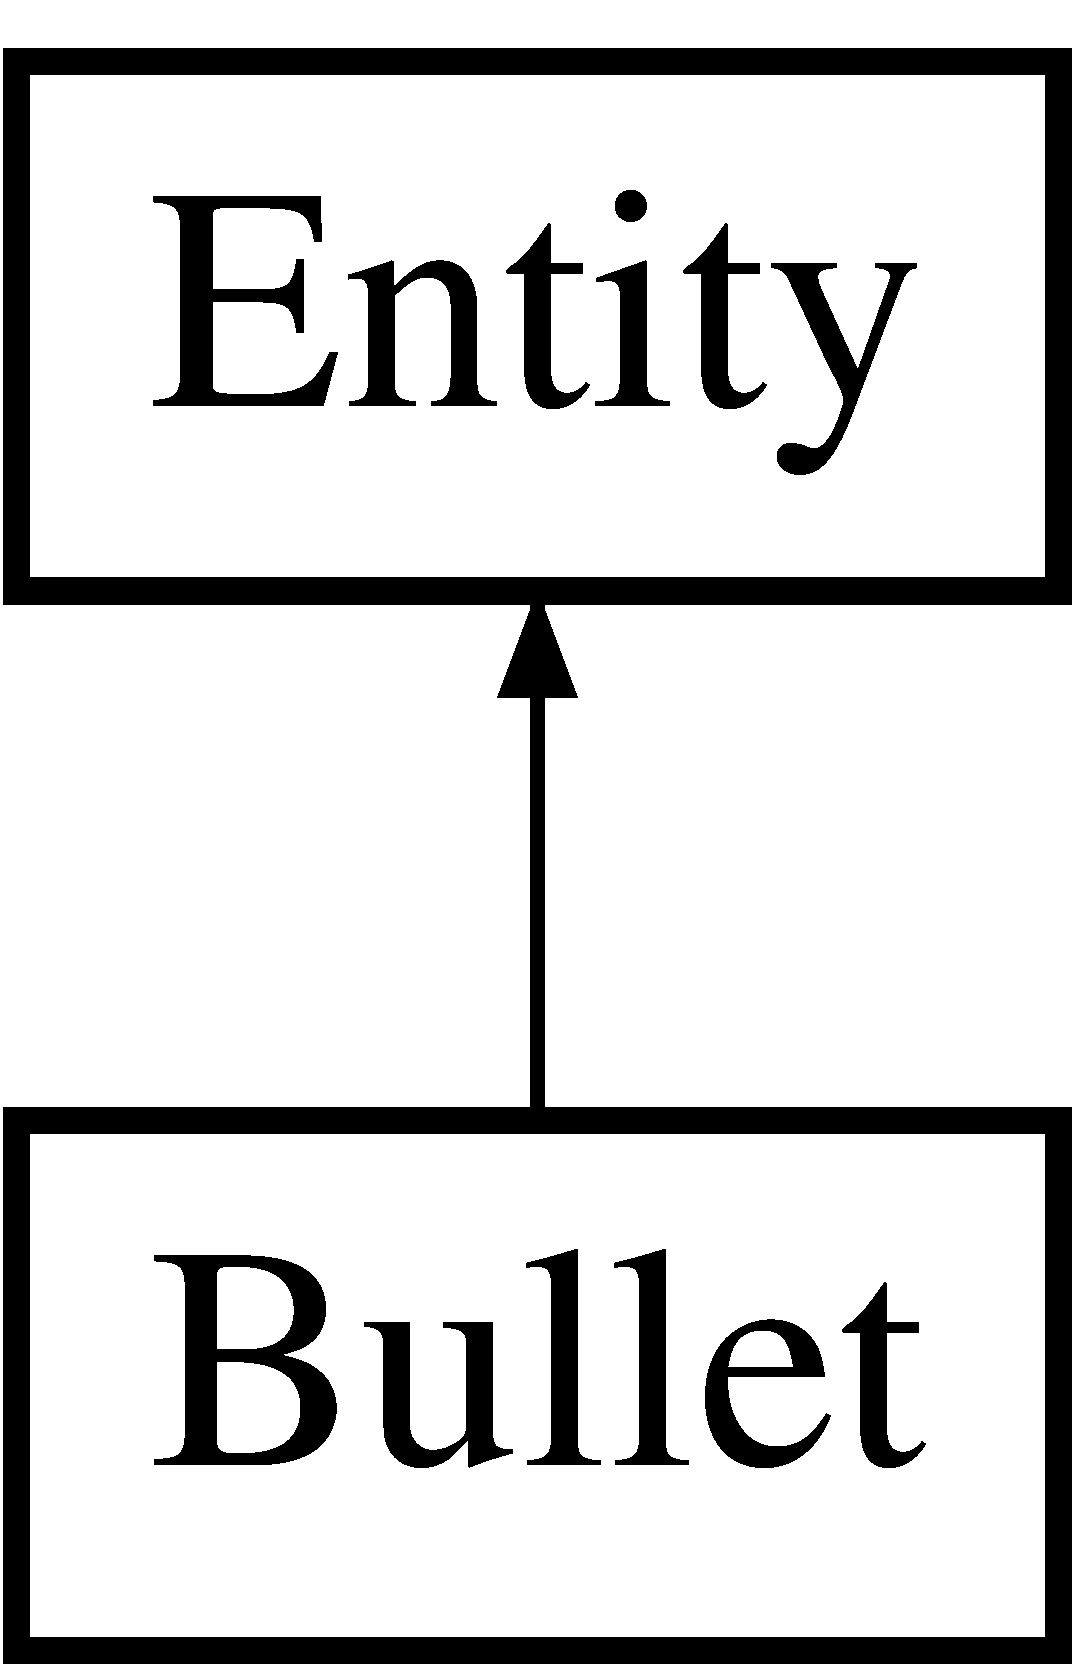
\includegraphics[height=2.000000cm]{class_bullet}
\end{center}
\end{figure}
\subsection*{Public Member Functions}
\begin{DoxyCompactItemize}
\item 
\hyperlink{class_bullet_a33aa7037c020e72ea614356dc1f7e67b}{Bullet} (float speed, Vector2f relative\+Pos\+Bul, Vector2f \hyperlink{class_entity_a6af9d6498134ad0906011778bc5736db}{position}, Vector2f \hyperlink{class_entity_ae9a0a364c85f91ade5088b3610131417}{size}, bool \hyperlink{class_entity_af1b0754c9d5f4afa73834b23c6437101}{is\+Solid}=true, int \hyperlink{class_entity_a4edd9cc2506add0d9e27fade0bf957e8}{state}=2)
\item 
\hyperlink{class_bullet_aaeb5cb41d7db89f49007b08b41f1bfcf}{$\sim$\+Bullet} ()
\item 
bool \hyperlink{class_bullet_a86ab78893d4a171e3215486efc6dc66b}{get\+Is\+Alive} ()
\begin{DoxyCompactList}\small\item\em /getter to know if bullet still is active \end{DoxyCompactList}\item 
void \hyperlink{class_bullet_a2f178ec7de59d5ff1edd975065b4f279}{set\+Is\+Alive} (bool b)
\begin{DoxyCompactList}\small\item\em setter to set bullet active or inactive \end{DoxyCompactList}\item 
Vector2f \hyperlink{class_bullet_a6b6acf4d172bc98a9371cc431eca4e0d}{get\+Direction} ()
\begin{DoxyCompactList}\small\item\em get the direction where the bullet will be after the next update \end{DoxyCompactList}\item 
void \hyperlink{class_bullet_a32f4a0611fe2dd245fee955d14ca1f68}{update} ()
\begin{DoxyCompactList}\small\item\em update the position of the bullet \end{DoxyCompactList}\item 
void \hyperlink{class_bullet_a14a795a7a6f4d0ad2e96a19b79afc5ee}{draw} (Render\+Window \&window)
\begin{DoxyCompactList}\small\item\em draws the bullet on the window \end{DoxyCompactList}\item 
int \hyperlink{class_bullet_a61627cf61a12182a8b8ac9c8a9277de5}{get\+Time\+Alive} ()
\end{DoxyCompactItemize}
\subsection*{Additional Inherited Members}


\subsection{Detailed Description}
A bullet object is an entity that`s always moving in one direction. 

the buller class contains the item graphic and overrides the necessary functions from \hyperlink{class_entity}{Entity}. the direction, speed and rotation will be calculated in the constructur. when the bullet is inactive it will stop drawing and calculating the next position. if the bullet exist longer than 15 seconds it will go automaticly in\+Active 

Definition at line 20 of file bullet.\+h.



\subsection{Constructor \& Destructor Documentation}
\mbox{\Hypertarget{class_bullet_a33aa7037c020e72ea614356dc1f7e67b}\label{class_bullet_a33aa7037c020e72ea614356dc1f7e67b}} 
\index{Bullet@{Bullet}!Bullet@{Bullet}}
\index{Bullet@{Bullet}!Bullet@{Bullet}}
\subsubsection{\texorpdfstring{Bullet()}{Bullet()}}
{\footnotesize\ttfamily Bullet\+::\+Bullet (\begin{DoxyParamCaption}\item[{float}]{speed,  }\item[{Vector2f}]{relative\+Pos\+Bul,  }\item[{Vector2f}]{position,  }\item[{Vector2f}]{size,  }\item[{bool}]{is\+Solid = {\ttfamily true},  }\item[{int}]{state = {\ttfamily 2} }\end{DoxyParamCaption})}

/ float speed speed in pixels /\+Vector2f relative\+Pos\+Bul the vector with the spawn point as zero point to set the direction / Vector2f position the spawn point / Vector2f size size of bullet / bool is\+Solid 

Definition at line 5 of file bullet.\+cpp.

\mbox{\Hypertarget{class_bullet_aaeb5cb41d7db89f49007b08b41f1bfcf}\label{class_bullet_aaeb5cb41d7db89f49007b08b41f1bfcf}} 
\index{Bullet@{Bullet}!````~Bullet@{$\sim$\+Bullet}}
\index{````~Bullet@{$\sim$\+Bullet}!Bullet@{Bullet}}
\subsubsection{\texorpdfstring{$\sim$\+Bullet()}{~Bullet()}}
{\footnotesize\ttfamily Bullet\+::$\sim$\+Bullet (\begin{DoxyParamCaption}{ }\end{DoxyParamCaption})}



Definition at line 15 of file bullet.\+cpp.



\subsection{Member Function Documentation}
\mbox{\Hypertarget{class_bullet_a14a795a7a6f4d0ad2e96a19b79afc5ee}\label{class_bullet_a14a795a7a6f4d0ad2e96a19b79afc5ee}} 
\index{Bullet@{Bullet}!draw@{draw}}
\index{draw@{draw}!Bullet@{Bullet}}
\subsubsection{\texorpdfstring{draw()}{draw()}}
{\footnotesize\ttfamily void Bullet\+::draw (\begin{DoxyParamCaption}\item[{Render\+Window \&}]{window }\end{DoxyParamCaption})\hspace{0.3cm}{\ttfamily [virtual]}}



draws the bullet on the window 

Render\+Window window window to draw in 

Reimplemented from \hyperlink{class_entity_a030c3aa6641df7981a2d8a3fba890ec7}{Entity}.



Definition at line 52 of file bullet.\+cpp.

\mbox{\Hypertarget{class_bullet_a6b6acf4d172bc98a9371cc431eca4e0d}\label{class_bullet_a6b6acf4d172bc98a9371cc431eca4e0d}} 
\index{Bullet@{Bullet}!get\+Direction@{get\+Direction}}
\index{get\+Direction@{get\+Direction}!Bullet@{Bullet}}
\subsubsection{\texorpdfstring{get\+Direction()}{getDirection()}}
{\footnotesize\ttfamily Vector2f Bullet\+::get\+Direction (\begin{DoxyParamCaption}{ }\end{DoxyParamCaption})}



get the direction where the bullet will be after the next update 

Vector2f \hyperlink{class_bullet_a6b6acf4d172bc98a9371cc431eca4e0d}{get\+Direction()}; 

Definition at line 44 of file bullet.\+cpp.

\mbox{\Hypertarget{class_bullet_a86ab78893d4a171e3215486efc6dc66b}\label{class_bullet_a86ab78893d4a171e3215486efc6dc66b}} 
\index{Bullet@{Bullet}!get\+Is\+Alive@{get\+Is\+Alive}}
\index{get\+Is\+Alive@{get\+Is\+Alive}!Bullet@{Bullet}}
\subsubsection{\texorpdfstring{get\+Is\+Alive()}{getIsAlive()}}
{\footnotesize\ttfamily bool Bullet\+::get\+Is\+Alive (\begin{DoxyParamCaption}{ }\end{DoxyParamCaption})}



/getter to know if bullet still is active 

bool \hyperlink{class_bullet_a86ab78893d4a171e3215486efc6dc66b}{get\+Is\+Alive()}; 

Definition at line 40 of file bullet.\+cpp.

\mbox{\Hypertarget{class_bullet_a61627cf61a12182a8b8ac9c8a9277de5}\label{class_bullet_a61627cf61a12182a8b8ac9c8a9277de5}} 
\index{Bullet@{Bullet}!get\+Time\+Alive@{get\+Time\+Alive}}
\index{get\+Time\+Alive@{get\+Time\+Alive}!Bullet@{Bullet}}
\subsubsection{\texorpdfstring{get\+Time\+Alive()}{getTimeAlive()}}
{\footnotesize\ttfamily int Bullet\+::get\+Time\+Alive (\begin{DoxyParamCaption}{ }\end{DoxyParamCaption})}

\textbackslash{} brief get the time the bullet is active 

Definition at line 48 of file bullet.\+cpp.

\mbox{\Hypertarget{class_bullet_a2f178ec7de59d5ff1edd975065b4f279}\label{class_bullet_a2f178ec7de59d5ff1edd975065b4f279}} 
\index{Bullet@{Bullet}!set\+Is\+Alive@{set\+Is\+Alive}}
\index{set\+Is\+Alive@{set\+Is\+Alive}!Bullet@{Bullet}}
\subsubsection{\texorpdfstring{set\+Is\+Alive()}{setIsAlive()}}
{\footnotesize\ttfamily void Bullet\+::set\+Is\+Alive (\begin{DoxyParamCaption}\item[{bool}]{b }\end{DoxyParamCaption})}



setter to set bullet active or inactive 

void \hyperlink{class_bullet_a2f178ec7de59d5ff1edd975065b4f279}{set\+Is\+Alive(bool b)}; 

Definition at line 36 of file bullet.\+cpp.

\mbox{\Hypertarget{class_bullet_a32f4a0611fe2dd245fee955d14ca1f68}\label{class_bullet_a32f4a0611fe2dd245fee955d14ca1f68}} 
\index{Bullet@{Bullet}!update@{update}}
\index{update@{update}!Bullet@{Bullet}}
\subsubsection{\texorpdfstring{update()}{update()}}
{\footnotesize\ttfamily void Bullet\+::update (\begin{DoxyParamCaption}{ }\end{DoxyParamCaption})\hspace{0.3cm}{\ttfamily [virtual]}}



update the position of the bullet 

void \hyperlink{class_bullet_a32f4a0611fe2dd245fee955d14ca1f68}{update()} 

Reimplemented from \hyperlink{class_entity_aed73e98b980b85833428c935cc1c69f8}{Entity}.



Definition at line 24 of file bullet.\+cpp.



The documentation for this class was generated from the following files\+:\begin{DoxyCompactItemize}
\item 
C\+:/\+Users/joost/\+Documents/\+Git\+Hub/topdown/\+Code/\+Team\+Topdown/\+Team\+Topdown/\hyperlink{bullet_8h}{bullet.\+h}\item 
C\+:/\+Users/joost/\+Documents/\+Git\+Hub/topdown/\+Code/\+Team\+Topdown/\+Team\+Topdown/\hyperlink{bullet_8cpp}{bullet.\+cpp}\end{DoxyCompactItemize}

\hypertarget{class_camera}{}\section{Camera Class Reference}
\label{class_camera}\index{Camera@{Camera}}


{\ttfamily \#include $<$Camera.\+h$>$}

\subsection*{Public Member Functions}
\begin{DoxyCompactItemize}
\item 
\hyperlink{class_camera_a96a2da7cc4bb17b4a68ae236528c1b47}{Camera} (View \&view, \hyperlink{class_player}{Player} \&obj\+To\+Follow, Render\+Window \&window, const Vector2f \&size\+Map)
\begin{DoxyCompactList}\small\item\em Create a \hyperlink{class_camera}{Camera} to follow the player. \end{DoxyCompactList}\item 
void \hyperlink{class_camera_a42cda7239981a5618660d04bd5893556}{update} ()
\begin{DoxyCompactList}\small\item\em set the camera at the good position \end{DoxyCompactList}\item 
void \hyperlink{class_camera_aa4a2ea30c94998c0222fdffe02a499f1}{set\+Timer} (\hyperlink{struct_timer}{Timer} \&t)
\item 
View \hyperlink{class_camera_a14474d1aabd7268f7aa922fe30647365}{Get\+View} ()
\item 
Vector2f \hyperlink{class_camera_ab3b9ec6e34ef3b004d9061d96d71302f}{get\+Position} ()
\end{DoxyCompactItemize}


\subsection{Detailed Description}


Definition at line 13 of file Camera.\+h.



\subsection{Constructor \& Destructor Documentation}
\mbox{\Hypertarget{class_camera_a96a2da7cc4bb17b4a68ae236528c1b47}\label{class_camera_a96a2da7cc4bb17b4a68ae236528c1b47}} 
\index{Camera@{Camera}!Camera@{Camera}}
\index{Camera@{Camera}!Camera@{Camera}}
\subsubsection{\texorpdfstring{Camera()}{Camera()}}
{\footnotesize\ttfamily Camera\+::\+Camera (\begin{DoxyParamCaption}\item[{View \&}]{view,  }\item[{\hyperlink{class_player}{Player} \&}]{obj\+To\+Follow,  }\item[{Render\+Window \&}]{window,  }\item[{const Vector2f \&}]{size\+Map }\end{DoxyParamCaption})}



Create a \hyperlink{class_camera}{Camera} to follow the player. 

View view the view object Window window Vector2f size\+Map The vector of the size of the background image 

Definition at line 4 of file Camera.\+cpp.



\subsection{Member Function Documentation}
\mbox{\Hypertarget{class_camera_ab3b9ec6e34ef3b004d9061d96d71302f}\label{class_camera_ab3b9ec6e34ef3b004d9061d96d71302f}} 
\index{Camera@{Camera}!get\+Position@{get\+Position}}
\index{get\+Position@{get\+Position}!Camera@{Camera}}
\subsubsection{\texorpdfstring{get\+Position()}{getPosition()}}
{\footnotesize\ttfamily Vector2f Camera\+::get\+Position (\begin{DoxyParamCaption}{ }\end{DoxyParamCaption})}

/\+View get\+Position /brief returns a Vector2f for the center of the view linked to this. 

Definition at line 34 of file Camera.\+cpp.

\mbox{\Hypertarget{class_camera_a14474d1aabd7268f7aa922fe30647365}\label{class_camera_a14474d1aabd7268f7aa922fe30647365}} 
\index{Camera@{Camera}!Get\+View@{Get\+View}}
\index{Get\+View@{Get\+View}!Camera@{Camera}}
\subsubsection{\texorpdfstring{Get\+View()}{GetView()}}
{\footnotesize\ttfamily View Camera\+::\+Get\+View (\begin{DoxyParamCaption}{ }\end{DoxyParamCaption})}

/\+View Get\+View /brief returns the View of the view linked to this. 

Definition at line 29 of file Camera.\+cpp.

\mbox{\Hypertarget{class_camera_aa4a2ea30c94998c0222fdffe02a499f1}\label{class_camera_aa4a2ea30c94998c0222fdffe02a499f1}} 
\index{Camera@{Camera}!set\+Timer@{set\+Timer}}
\index{set\+Timer@{set\+Timer}!Camera@{Camera}}
\subsubsection{\texorpdfstring{set\+Timer()}{setTimer()}}
{\footnotesize\ttfamily void Camera\+::set\+Timer (\begin{DoxyParamCaption}\item[{\hyperlink{struct_timer}{Timer} \&}]{t }\end{DoxyParamCaption})}

/void set\+Timer /brief links the shake\+Timer to that of another so the shaking of the screen can be initiated elsewhere. 

Definition at line 25 of file Camera.\+cpp.

\mbox{\Hypertarget{class_camera_a42cda7239981a5618660d04bd5893556}\label{class_camera_a42cda7239981a5618660d04bd5893556}} 
\index{Camera@{Camera}!update@{update}}
\index{update@{update}!Camera@{Camera}}
\subsubsection{\texorpdfstring{update()}{update()}}
{\footnotesize\ttfamily void Camera\+::update (\begin{DoxyParamCaption}{ }\end{DoxyParamCaption})}



set the camera at the good position 

void \hyperlink{class_camera_a42cda7239981a5618660d04bd5893556}{update()};

set camera in such a postion that the player will be in the center unless the player is at a boundry of the map 

Definition at line 14 of file Camera.\+cpp.



The documentation for this class was generated from the following files\+:\begin{DoxyCompactItemize}
\item 
C\+:/\+Users/joost/\+Documents/\+Git\+Hub/topdown/\+Code/\+Team\+Topdown/\+Team\+Topdown/\hyperlink{_camera_8h}{Camera.\+h}\item 
C\+:/\+Users/joost/\+Documents/\+Git\+Hub/topdown/\+Code/\+Team\+Topdown/\+Team\+Topdown/\hyperlink{_camera_8cpp}{Camera.\+cpp}\end{DoxyCompactItemize}

\hypertarget{class_clickable_button}{}\section{Clickable\+Button Class Reference}
\label{class_clickable_button}\index{Clickable\+Button@{Clickable\+Button}}


A clickable button with text, animation and auto-\/resize to text width.  




{\ttfamily \#include $<$Clickable\+Button.\+hpp$>$}

Inheritance diagram for Clickable\+Button\+:\begin{figure}[H]
\begin{center}
\leavevmode
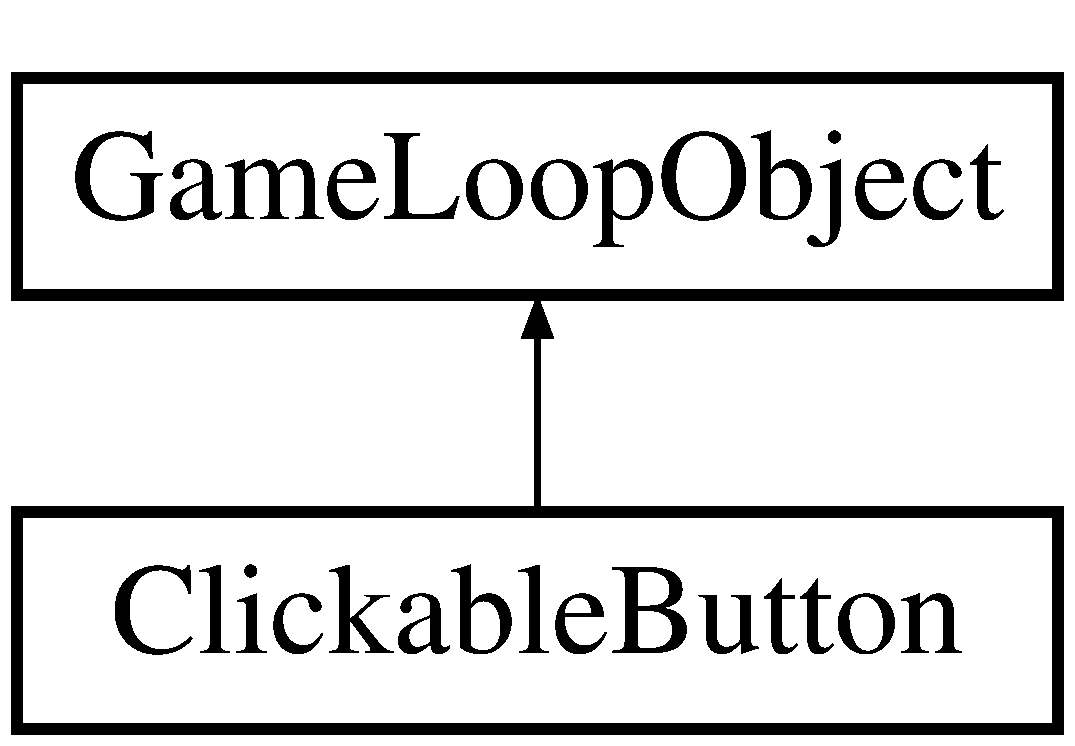
\includegraphics[height=2.000000cm]{class_clickable_button}
\end{center}
\end{figure}
\subsection*{Public Member Functions}
\begin{DoxyCompactItemize}
\item 
\hyperlink{class_clickable_button_a2941caf8b0b04291cb6ae09df4deb5aa}{Clickable\+Button} (sf\+::\+Render\+Window \&window, sf\+::\+Vector2f position, sf\+::\+Vector2f size, std\+::string text, bool auto\+Calc\+Width=0)
\begin{DoxyCompactList}\small\item\em Constructor. \end{DoxyCompactList}\item 
void \hyperlink{class_clickable_button_a939a1f2a5414c37e9c1c1310db576224}{Handle\+Input} ()
\begin{DoxyCompactList}\small\item\em The method to handle user input (currently only mouse input). \end{DoxyCompactList}\item 
void \hyperlink{class_clickable_button_a393e1529583626f6ee52f0955bd68da8}{Update} ()
\begin{DoxyCompactList}\small\item\em The button\textquotesingle{}s update method. \end{DoxyCompactList}\item 
void \hyperlink{class_clickable_button_a55b5a7b941f25066a8d0481326794b62}{Draw} (sf\+::\+Render\+Window \&window)
\begin{DoxyCompactList}\small\item\em The button\textquotesingle{}s draw method. \end{DoxyCompactList}\item 
void \hyperlink{class_clickable_button_a01ae3f140debdc8b525e1ef745bdbff3}{Reset} ()
\begin{DoxyCompactList}\small\item\em The button\textquotesingle{}s reset method. \end{DoxyCompactList}\item 
void \hyperlink{class_clickable_button_a433c3e53d1ebf7b1ca847e90240b2a5c}{Auto\+Calc\+Width} (std\+::string str)
\begin{DoxyCompactList}\small\item\em This method recalculates the button\textquotesingle{}s width based on the button\textquotesingle{}s text. \end{DoxyCompactList}\item 
void \hyperlink{class_clickable_button_af39cab51ca37c5465bbfec0e5268b768}{Auto\+Calc\+Width\+Menu} (std\+::string str)
\begin{DoxyCompactList}\small\item\em The Auto\+Calc\+Width method if the button is part of a menu. \end{DoxyCompactList}\item 
int \hyperlink{class_clickable_button_a45a3f33e2e11191afb413617a665d2f5}{Get\+Width} ()
\begin{DoxyCompactList}\small\item\em Returns the width of the button as an int. \end{DoxyCompactList}\item 
bool \hyperlink{class_clickable_button_aa63eaa88bbfaf717e46b5ab4cfa6d12c}{Is\+Pressed} ()
\begin{DoxyCompactList}\small\item\em Checks if the button is pressed and returns a bool accordingly. \end{DoxyCompactList}\item 
void \hyperlink{class_clickable_button_ae96a7ed06c7eb63b37eefeb45407426e}{Reposition\+To\+Center} (sf\+::\+Vector2f screen\+Origin, int height)
\begin{DoxyCompactList}\small\item\em Repositions the button\textquotesingle{}s origin to the center of the screen. \end{DoxyCompactList}\end{DoxyCompactItemize}


\subsection{Detailed Description}
A clickable button with text, animation and auto-\/resize to text width. 

A clickable button. Has an idle,\textquotesingle{}on-\/hover\textquotesingle{} and pressed state and changes sprites accordingly. Can be auto-\/resized to text length if desired. The pressed state can be read by calling the \hyperlink{class_clickable_button_aa63eaa88bbfaf717e46b5ab4cfa6d12c}{Is\+Pressed()} method. Sound effects play when hovering over the button and when successfully pressing the button. 

Definition at line 14 of file Clickable\+Button.\+hpp.



\subsection{Constructor \& Destructor Documentation}
\mbox{\Hypertarget{class_clickable_button_a2941caf8b0b04291cb6ae09df4deb5aa}\label{class_clickable_button_a2941caf8b0b04291cb6ae09df4deb5aa}} 
\index{Clickable\+Button@{Clickable\+Button}!Clickable\+Button@{Clickable\+Button}}
\index{Clickable\+Button@{Clickable\+Button}!Clickable\+Button@{Clickable\+Button}}
\subsubsection{\texorpdfstring{Clickable\+Button()}{ClickableButton()}}
{\footnotesize\ttfamily Clickable\+Button\+::\+Clickable\+Button (\begin{DoxyParamCaption}\item[{sf\+::\+Render\+Window \&}]{window,  }\item[{sf\+::\+Vector2f}]{position,  }\item[{sf\+::\+Vector2f}]{size,  }\item[{std\+::string}]{text,  }\item[{bool}]{auto\+Calc\+Width = {\ttfamily 0} }\end{DoxyParamCaption})}



Constructor. 

To create a button, it needs a window (to read mouseposition), a position, a desired size (length and width), a text to draw on the button and, optionally, either a true or a false if the button should be resized automatically to text length (false by default). If this is set to true, the x value of size is ignored and calculated by the button itself. if the optional bool auto\+Calc\+Width is set to true, the x value of the input vector size is ignored and is calculated based on the text length. 

Definition at line 5 of file Clickable\+Button.\+cpp.



\subsection{Member Function Documentation}
\mbox{\Hypertarget{class_clickable_button_a433c3e53d1ebf7b1ca847e90240b2a5c}\label{class_clickable_button_a433c3e53d1ebf7b1ca847e90240b2a5c}} 
\index{Clickable\+Button@{Clickable\+Button}!Auto\+Calc\+Width@{Auto\+Calc\+Width}}
\index{Auto\+Calc\+Width@{Auto\+Calc\+Width}!Clickable\+Button@{Clickable\+Button}}
\subsubsection{\texorpdfstring{Auto\+Calc\+Width()}{AutoCalcWidth()}}
{\footnotesize\ttfamily void Clickable\+Button\+::\+Auto\+Calc\+Width (\begin{DoxyParamCaption}\item[{std\+::string}]{str }\end{DoxyParamCaption})}



This method recalculates the button\textquotesingle{}s width based on the button\textquotesingle{}s text. 

\textquotesingle{}nuff said. 

Definition at line 118 of file Clickable\+Button.\+cpp.

\mbox{\Hypertarget{class_clickable_button_af39cab51ca37c5465bbfec0e5268b768}\label{class_clickable_button_af39cab51ca37c5465bbfec0e5268b768}} 
\index{Clickable\+Button@{Clickable\+Button}!Auto\+Calc\+Width\+Menu@{Auto\+Calc\+Width\+Menu}}
\index{Auto\+Calc\+Width\+Menu@{Auto\+Calc\+Width\+Menu}!Clickable\+Button@{Clickable\+Button}}
\subsubsection{\texorpdfstring{Auto\+Calc\+Width\+Menu()}{AutoCalcWidthMenu()}}
{\footnotesize\ttfamily void Clickable\+Button\+::\+Auto\+Calc\+Width\+Menu (\begin{DoxyParamCaption}\item[{std\+::string}]{str }\end{DoxyParamCaption})}



The Auto\+Calc\+Width method if the button is part of a menu. 

This method does the same as Auto\+Calc\+Width, but is used when the button is part of a menu. A menu is drawn based on its origin\textquotesingle{}s x-\/value, while a regular button is drawn from the top left corner instead of origin. This means the button\textquotesingle{}s position also has to be recalculated if it is part of a menu. This method is only called in the menu class, never in the button\textquotesingle{}s class itself. 

Definition at line 125 of file Clickable\+Button.\+cpp.

\mbox{\Hypertarget{class_clickable_button_a55b5a7b941f25066a8d0481326794b62}\label{class_clickable_button_a55b5a7b941f25066a8d0481326794b62}} 
\index{Clickable\+Button@{Clickable\+Button}!Draw@{Draw}}
\index{Draw@{Draw}!Clickable\+Button@{Clickable\+Button}}
\subsubsection{\texorpdfstring{Draw()}{Draw()}}
{\footnotesize\ttfamily void Clickable\+Button\+::\+Draw (\begin{DoxyParamCaption}\item[{sf\+::\+Render\+Window \&}]{window }\end{DoxyParamCaption})\hspace{0.3cm}{\ttfamily [virtual]}}



The button\textquotesingle{}s draw method. 

First draws the button\textquotesingle{}s sprite, then draws the button\textquotesingle{}s text on top. 

Reimplemented from \hyperlink{class_game_loop_object_a0572a88e5b98fa8a41078260d152202d}{Game\+Loop\+Object}.

\mbox{\Hypertarget{class_clickable_button_a45a3f33e2e11191afb413617a665d2f5}\label{class_clickable_button_a45a3f33e2e11191afb413617a665d2f5}} 
\index{Clickable\+Button@{Clickable\+Button}!Get\+Width@{Get\+Width}}
\index{Get\+Width@{Get\+Width}!Clickable\+Button@{Clickable\+Button}}
\subsubsection{\texorpdfstring{Get\+Width()}{GetWidth()}}
{\footnotesize\ttfamily int Clickable\+Button\+::\+Get\+Width (\begin{DoxyParamCaption}{ }\end{DoxyParamCaption})}



Returns the width of the button as an int. 

\textquotesingle{}nuff said. 

Definition at line 136 of file Clickable\+Button.\+cpp.

\mbox{\Hypertarget{class_clickable_button_a939a1f2a5414c37e9c1c1310db576224}\label{class_clickable_button_a939a1f2a5414c37e9c1c1310db576224}} 
\index{Clickable\+Button@{Clickable\+Button}!Handle\+Input@{Handle\+Input}}
\index{Handle\+Input@{Handle\+Input}!Clickable\+Button@{Clickable\+Button}}
\subsubsection{\texorpdfstring{Handle\+Input()}{HandleInput()}}
{\footnotesize\ttfamily void Clickable\+Button\+::\+Handle\+Input (\begin{DoxyParamCaption}{ }\end{DoxyParamCaption})\hspace{0.3cm}{\ttfamily [virtual]}}



The method to handle user input (currently only mouse input). 

This method reads if the mouse is hovering over a button, if a button is pressed + being held, if pressing is canceled (moving the mouse away from the button while holding and then releasing), and if a button is successfully pressed. Textures are then updated accordingly. 

Reimplemented from \hyperlink{class_game_loop_object_aecab111d504b7f4590045ca7c83a36de}{Game\+Loop\+Object}.



Definition at line 49 of file Clickable\+Button.\+cpp.

\mbox{\Hypertarget{class_clickable_button_aa63eaa88bbfaf717e46b5ab4cfa6d12c}\label{class_clickable_button_aa63eaa88bbfaf717e46b5ab4cfa6d12c}} 
\index{Clickable\+Button@{Clickable\+Button}!Is\+Pressed@{Is\+Pressed}}
\index{Is\+Pressed@{Is\+Pressed}!Clickable\+Button@{Clickable\+Button}}
\subsubsection{\texorpdfstring{Is\+Pressed()}{IsPressed()}}
{\footnotesize\ttfamily bool Clickable\+Button\+::\+Is\+Pressed (\begin{DoxyParamCaption}{ }\end{DoxyParamCaption})}



Checks if the button is pressed and returns a bool accordingly. 

If the button is pressed, it is first reset to its unpressed state, then \textquotesingle{}true\textquotesingle{} is returned. Else, false is returned. 

Definition at line 141 of file Clickable\+Button.\+cpp.

\mbox{\Hypertarget{class_clickable_button_ae96a7ed06c7eb63b37eefeb45407426e}\label{class_clickable_button_ae96a7ed06c7eb63b37eefeb45407426e}} 
\index{Clickable\+Button@{Clickable\+Button}!Reposition\+To\+Center@{Reposition\+To\+Center}}
\index{Reposition\+To\+Center@{Reposition\+To\+Center}!Clickable\+Button@{Clickable\+Button}}
\subsubsection{\texorpdfstring{Reposition\+To\+Center()}{RepositionToCenter()}}
{\footnotesize\ttfamily void Clickable\+Button\+::\+Reposition\+To\+Center (\begin{DoxyParamCaption}\item[{sf\+::\+Vector2f}]{screen\+Origin,  }\item[{int}]{height }\end{DoxyParamCaption})}



Repositions the button\textquotesingle{}s origin to the center of the screen. 

Method used by the menu class to reposition the origins of buttons to the center of the screen when making a pause menu. 

Definition at line 150 of file Clickable\+Button.\+cpp.

\mbox{\Hypertarget{class_clickable_button_a01ae3f140debdc8b525e1ef745bdbff3}\label{class_clickable_button_a01ae3f140debdc8b525e1ef745bdbff3}} 
\index{Clickable\+Button@{Clickable\+Button}!Reset@{Reset}}
\index{Reset@{Reset}!Clickable\+Button@{Clickable\+Button}}
\subsubsection{\texorpdfstring{Reset()}{Reset()}}
{\footnotesize\ttfamily void Clickable\+Button\+::\+Reset (\begin{DoxyParamCaption}{ }\end{DoxyParamCaption})\hspace{0.3cm}{\ttfamily [virtual]}}



The button\textquotesingle{}s reset method. 

Does nothing. 

Reimplemented from \hyperlink{class_game_loop_object_af61e973be170cb9437a5b7d9ecd6ef53}{Game\+Loop\+Object}.

\mbox{\Hypertarget{class_clickable_button_a393e1529583626f6ee52f0955bd68da8}\label{class_clickable_button_a393e1529583626f6ee52f0955bd68da8}} 
\index{Clickable\+Button@{Clickable\+Button}!Update@{Update}}
\index{Update@{Update}!Clickable\+Button@{Clickable\+Button}}
\subsubsection{\texorpdfstring{Update()}{Update()}}
{\footnotesize\ttfamily void Clickable\+Button\+::\+Update (\begin{DoxyParamCaption}{ }\end{DoxyParamCaption})\hspace{0.3cm}{\ttfamily [virtual]}}



The button\textquotesingle{}s update method. 

Does nothing, as everything else is handled in the Handle\+Input method. 

Reimplemented from \hyperlink{class_game_loop_object_ae36a15981f1dd3f3bea6050473490349}{Game\+Loop\+Object}.



Definition at line 108 of file Clickable\+Button.\+cpp.



The documentation for this class was generated from the following files\+:\begin{DoxyCompactItemize}
\item 
C\+:/\+Users/joost/\+Documents/\+Git\+Hub/topdown/\+Code/\+Team\+Topdown/\+Team\+Topdown/\hyperlink{_clickable_button_8hpp}{Clickable\+Button.\+hpp}\item 
C\+:/\+Users/joost/\+Documents/\+Git\+Hub/topdown/\+Code/\+Team\+Topdown/\+Team\+Topdown/\hyperlink{_clickable_button_8cpp}{Clickable\+Button.\+cpp}\end{DoxyCompactItemize}

\hypertarget{classcontrols_controller}{}\section{controls\+Controller Class Reference}
\label{classcontrols_controller}\index{controls\+Controller@{controls\+Controller}}


updates data from \hyperlink{classcontrols_handler}{controls\+Handler} to \hyperlink{classcontrols_input}{controls\+Input}  




{\ttfamily \#include $<$controls\+Controller.\+h$>$}



\subsection{Detailed Description}
updates data from \hyperlink{classcontrols_handler}{controls\+Handler} to \hyperlink{classcontrols_input}{controls\+Input} 

The documentation for this class was generated from the following file\+:\begin{DoxyCompactItemize}
\item 
C\+:/\+Users/joost/\+Documents/\+Git\+Hub/topdown/\+Code/\+Team\+Topdown/\+Team\+Topdown/\hyperlink{controls_controller_8h}{controls\+Controller.\+h}\end{DoxyCompactItemize}

\hypertarget{class_controls_controller}{}\section{Controls\+Controller Class Reference}
\label{class_controls_controller}\index{Controls\+Controller@{Controls\+Controller}}


{\ttfamily \#include $<$controls\+Controller.\+h$>$}

\subsection*{Public Member Functions}
\begin{DoxyCompactItemize}
\item 
\hyperlink{class_controls_controller_a560244e70655e8b4f54d8da805c9c2a6}{Controls\+Controller} (\hyperlink{struct_controls_input}{Controls\+Input} \&inpt, Window \&w)
\item 
void \hyperlink{class_controls_controller_a29b1ad7f93658a74035900645d59d9f7}{update} ()
\end{DoxyCompactItemize}


\subsection{Detailed Description}


Definition at line 26 of file controls\+Controller.\+h.



\subsection{Constructor \& Destructor Documentation}
\mbox{\Hypertarget{class_controls_controller_a560244e70655e8b4f54d8da805c9c2a6}\label{class_controls_controller_a560244e70655e8b4f54d8da805c9c2a6}} 
\index{Controls\+Controller@{Controls\+Controller}!Controls\+Controller@{Controls\+Controller}}
\index{Controls\+Controller@{Controls\+Controller}!Controls\+Controller@{Controls\+Controller}}
\subsubsection{\texorpdfstring{Controls\+Controller()}{ControlsController()}}
{\footnotesize\ttfamily Controls\+Controller\+::\+Controls\+Controller (\begin{DoxyParamCaption}\item[{\hyperlink{struct_controls_input}{Controls\+Input} \&}]{inpt,  }\item[{Window \&}]{w }\end{DoxyParamCaption})}

/constructor \hyperlink{class_controls_controller}{Controls\+Controller} /brief makes a controller that controls controls. requires a \hyperlink{struct_controls_input}{Controls\+Input} and window object to record and save keyboard inputs. 

Definition at line 16 of file controls\+Controller.\+cpp.



\subsection{Member Function Documentation}
\mbox{\Hypertarget{class_controls_controller_a29b1ad7f93658a74035900645d59d9f7}\label{class_controls_controller_a29b1ad7f93658a74035900645d59d9f7}} 
\index{Controls\+Controller@{Controls\+Controller}!update@{update}}
\index{update@{update}!Controls\+Controller@{Controls\+Controller}}
\subsubsection{\texorpdfstring{update()}{update()}}
{\footnotesize\ttfamily void Controls\+Controller\+::update (\begin{DoxyParamCaption}{ }\end{DoxyParamCaption})}

/void \hyperlink{class_controls_controller_a29b1ad7f93658a74035900645d59d9f7}{update()} /brief updates \hyperlink{classcontrols_input}{controls\+Input} based on handler data. 

Definition at line 20 of file controls\+Controller.\+cpp.



The documentation for this class was generated from the following files\+:\begin{DoxyCompactItemize}
\item 
C\+:/\+Users/joost/\+Documents/\+Git\+Hub/topdown/\+Code/\+Team\+Topdown/\+Team\+Topdown/\hyperlink{controls_controller_8h}{controls\+Controller.\+h}\item 
C\+:/\+Users/joost/\+Documents/\+Git\+Hub/topdown/\+Code/\+Team\+Topdown/\+Team\+Topdown/\hyperlink{controls_controller_8cpp}{controls\+Controller.\+cpp}\end{DoxyCompactItemize}

\hypertarget{classcontrols_handler}{}\section{controls\+Handler Class Reference}
\label{classcontrols_handler}\index{controls\+Handler@{controls\+Handler}}


handles retrieving the data from hardware inputs  




{\ttfamily \#include $<$controls\+Controller.\+h$>$}



\subsection{Detailed Description}
handles retrieving the data from hardware inputs 

The documentation for this class was generated from the following file\+:\begin{DoxyCompactItemize}
\item 
C\+:/\+Users/joost/\+Documents/\+Git\+Hub/topdown/\+Code/\+Team\+Topdown/\+Team\+Topdown/\hyperlink{controls_controller_8h}{controls\+Controller.\+h}\end{DoxyCompactItemize}

\hypertarget{class_controls_handler}{}\section{Controls\+Handler Class Reference}
\label{class_controls_handler}\index{Controls\+Handler@{Controls\+Handler}}


{\ttfamily \#include $<$controls\+Controller.\+h$>$}

\subsection*{Public Member Functions}
\begin{DoxyCompactItemize}
\item 
\hyperlink{class_controls_handler_a49bf8377b225fa92ee71426d621825a0}{Controls\+Handler} ()
\item 
bool \hyperlink{class_controls_handler_a972e6c177eebdbe46033e39e64152f62}{get\+Key} (int key)
\end{DoxyCompactItemize}


\subsection{Detailed Description}


Definition at line 14 of file controls\+Controller.\+h.



\subsection{Constructor \& Destructor Documentation}
\mbox{\Hypertarget{class_controls_handler_a49bf8377b225fa92ee71426d621825a0}\label{class_controls_handler_a49bf8377b225fa92ee71426d621825a0}} 
\index{Controls\+Handler@{Controls\+Handler}!Controls\+Handler@{Controls\+Handler}}
\index{Controls\+Handler@{Controls\+Handler}!Controls\+Handler@{Controls\+Handler}}
\subsubsection{\texorpdfstring{Controls\+Handler()}{ControlsHandler()}}
{\footnotesize\ttfamily Controls\+Handler\+::\+Controls\+Handler (\begin{DoxyParamCaption}{ }\end{DoxyParamCaption})}

/constructor \hyperlink{class_controls_handler}{Controls\+Handler} /brief creates a C\+Ontrols\+Handler 

Definition at line 3 of file controls\+Controller.\+cpp.



\subsection{Member Function Documentation}
\mbox{\Hypertarget{class_controls_handler_a972e6c177eebdbe46033e39e64152f62}\label{class_controls_handler_a972e6c177eebdbe46033e39e64152f62}} 
\index{Controls\+Handler@{Controls\+Handler}!get\+Key@{get\+Key}}
\index{get\+Key@{get\+Key}!Controls\+Handler@{Controls\+Handler}}
\subsubsection{\texorpdfstring{get\+Key()}{getKey()}}
{\footnotesize\ttfamily bool Controls\+Handler\+::get\+Key (\begin{DoxyParamCaption}\item[{int}]{key }\end{DoxyParamCaption})}

gets keyboard int key state 

Definition at line 5 of file controls\+Controller.\+cpp.



The documentation for this class was generated from the following files\+:\begin{DoxyCompactItemize}
\item 
C\+:/\+Users/joost/\+Documents/\+Git\+Hub/topdown/\+Code/\+Team\+Topdown/\+Team\+Topdown/\hyperlink{controls_controller_8h}{controls\+Controller.\+h}\item 
C\+:/\+Users/joost/\+Documents/\+Git\+Hub/topdown/\+Code/\+Team\+Topdown/\+Team\+Topdown/\hyperlink{controls_controller_8cpp}{controls\+Controller.\+cpp}\end{DoxyCompactItemize}

\hypertarget{classcontrols_input}{}\section{controls\+Input Class Reference}
\label{classcontrols_input}\index{controls\+Input@{controls\+Input}}


struct with saves states of hardware inputs  




{\ttfamily \#include $<$controls\+Input.\+h$>$}



\subsection{Detailed Description}
struct with saves states of hardware inputs 

The documentation for this class was generated from the following file\+:\begin{DoxyCompactItemize}
\item 
C\+:/\+Users/joost/\+Documents/\+Git\+Hub/topdown/\+Code/\+Team\+Topdown/\+Team\+Topdown/\hyperlink{controls_input_8h}{controls\+Input.\+h}\end{DoxyCompactItemize}

\hypertarget{struct_controls_input}{}\section{Controls\+Input Struct Reference}
\label{struct_controls_input}\index{Controls\+Input@{Controls\+Input}}


{\ttfamily \#include $<$controls\+Input.\+h$>$}

\subsection*{Public Member Functions}
\begin{DoxyCompactItemize}
\item 
\hyperlink{struct_controls_input_a8df69a74d53e061f3b003a0a6709c1c7}{Controls\+Input} ()
\end{DoxyCompactItemize}
\subsection*{Public Attributes}
\begin{DoxyCompactItemize}
\item 
Vector2f \hyperlink{struct_controls_input_a9d2305fbda223544a306e37f2c9c89ec}{mouse\+Pos}
\item 
bool \hyperlink{struct_controls_input_adaef41f564822ecd14cc59ac5549f517}{w\+Key\+Pressed} = false
\item 
bool \hyperlink{struct_controls_input_a3d2a78cb660f43a9aec0cc2eff4102dd}{a\+Key\+Pressed} = false
\item 
bool \hyperlink{struct_controls_input_aa06968f2e5219f1e73be1c996268b5f9}{s\+Key\+Pressed} = false
\item 
bool \hyperlink{struct_controls_input_a6ce83f226b91636c1fd39990b58f392a}{d\+Key\+Pressed} = false
\item 
bool \hyperlink{struct_controls_input_a2e027179dcc06bdb10c74ccd4e7983e6}{p\+Key\+Pressed} = false
\item 
bool \hyperlink{struct_controls_input_a5005e6355bd91cbf3e32f75ee1324e7e}{num1\+Key\+Pressed} = false
\item 
bool \hyperlink{struct_controls_input_a3eb8030199fbda9eb2071e7e89c9cb07}{num2\+Key\+Pressed} = false
\item 
bool \hyperlink{struct_controls_input_a2b422f2d084970ac09c6a9b68aa03e22}{num3\+Key\+Pressed} = false
\item 
bool \hyperlink{struct_controls_input_aec8b1eccecbae03406e12a87b12520d9}{num4\+Key\+Pressed} = false
\item 
bool \hyperlink{struct_controls_input_aaf569ad5596dbb778880703879bbc765}{num5\+Key\+Pressed} = false
\item 
bool \hyperlink{struct_controls_input_a7835e1c719b55dc240e322486a4851c7}{num6\+Key\+Pressed} = false
\item 
bool \hyperlink{struct_controls_input_af7bf803f6c7b2e02ae83c85b42a965df}{num7\+Key\+Pressed} = false
\item 
bool \hyperlink{struct_controls_input_ab25d59fc0450d8880ada1bcbbccdd4a8}{num8\+Key\+Pressed} = false
\item 
bool \hyperlink{struct_controls_input_af0062f4839b149fe0c7402b74d883c7b}{num9\+Key\+Pressed} = false
\item 
bool \hyperlink{struct_controls_input_a22302eb427b7efc7cb629484e75aa0f9}{num0\+Key\+Pressed} = false
\item 
bool \hyperlink{struct_controls_input_a68b463995619f9b9a202dc84301728d0}{minus\+Key\+Pressed} = false
\item 
bool \hyperlink{struct_controls_input_ae4cfd2052a042c57c601ba2c3ed6fec1}{plus\+Key\+Pressed} = false
\item 
bool \hyperlink{struct_controls_input_a94141ee53845274d300476291bf74d7a}{shift\+Key\+Pressed} = false
\item 
bool \hyperlink{struct_controls_input_a36c963eb0406507823f8c69a8c68eba7}{space\+Key\+Pressed} = false
\item 
bool \hyperlink{struct_controls_input_a5026bb8fa2c88f2662eb1dba03599143}{enter\+Key\+Pressed} = false
\item 
bool \hyperlink{struct_controls_input_a5a220f2b624d21ac3ccb2f776a593305}{backspace\+Key\+Pressed} = false
\item 
bool \hyperlink{struct_controls_input_a8b7f874e66eeb9e038c80818feee81a1}{lmb\+Key\+Pressed} = false
\item 
bool \hyperlink{struct_controls_input_ae2486e484981cb64749c2119836687c0}{rmb\+Key\+Pressed} = false
\item 
bool \hyperlink{struct_controls_input_a24e3c06c9b3bbd1b6920bfd605f7390f}{r\+Key\+Pressed} = false
\end{DoxyCompactItemize}


\subsection{Detailed Description}


Definition at line 13 of file controls\+Input.\+h.



\subsection{Constructor \& Destructor Documentation}
\mbox{\Hypertarget{struct_controls_input_a8df69a74d53e061f3b003a0a6709c1c7}\label{struct_controls_input_a8df69a74d53e061f3b003a0a6709c1c7}} 
\index{Controls\+Input@{Controls\+Input}!Controls\+Input@{Controls\+Input}}
\index{Controls\+Input@{Controls\+Input}!Controls\+Input@{Controls\+Input}}
\subsubsection{\texorpdfstring{Controls\+Input()}{ControlsInput()}}
{\footnotesize\ttfamily Controls\+Input\+::\+Controls\+Input (\begin{DoxyParamCaption}{ }\end{DoxyParamCaption})}



Definition at line 4 of file controls\+Input.\+cpp.



\subsection{Member Data Documentation}
\mbox{\Hypertarget{struct_controls_input_a3d2a78cb660f43a9aec0cc2eff4102dd}\label{struct_controls_input_a3d2a78cb660f43a9aec0cc2eff4102dd}} 
\index{Controls\+Input@{Controls\+Input}!a\+Key\+Pressed@{a\+Key\+Pressed}}
\index{a\+Key\+Pressed@{a\+Key\+Pressed}!Controls\+Input@{Controls\+Input}}
\subsubsection{\texorpdfstring{a\+Key\+Pressed}{aKeyPressed}}
{\footnotesize\ttfamily bool Controls\+Input\+::a\+Key\+Pressed = false}

state of the L\+E\+FT key 

Definition at line 18 of file controls\+Input.\+h.

\mbox{\Hypertarget{struct_controls_input_a5a220f2b624d21ac3ccb2f776a593305}\label{struct_controls_input_a5a220f2b624d21ac3ccb2f776a593305}} 
\index{Controls\+Input@{Controls\+Input}!backspace\+Key\+Pressed@{backspace\+Key\+Pressed}}
\index{backspace\+Key\+Pressed@{backspace\+Key\+Pressed}!Controls\+Input@{Controls\+Input}}
\subsubsection{\texorpdfstring{backspace\+Key\+Pressed}{backspaceKeyPressed}}
{\footnotesize\ttfamily bool Controls\+Input\+::backspace\+Key\+Pressed = false}

state of the B\+A\+C\+K\+S\+P\+A\+CE key 

Definition at line 37 of file controls\+Input.\+h.

\mbox{\Hypertarget{struct_controls_input_a6ce83f226b91636c1fd39990b58f392a}\label{struct_controls_input_a6ce83f226b91636c1fd39990b58f392a}} 
\index{Controls\+Input@{Controls\+Input}!d\+Key\+Pressed@{d\+Key\+Pressed}}
\index{d\+Key\+Pressed@{d\+Key\+Pressed}!Controls\+Input@{Controls\+Input}}
\subsubsection{\texorpdfstring{d\+Key\+Pressed}{dKeyPressed}}
{\footnotesize\ttfamily bool Controls\+Input\+::d\+Key\+Pressed = false}

state of the R\+I\+G\+HT key 

Definition at line 20 of file controls\+Input.\+h.

\mbox{\Hypertarget{struct_controls_input_a5026bb8fa2c88f2662eb1dba03599143}\label{struct_controls_input_a5026bb8fa2c88f2662eb1dba03599143}} 
\index{Controls\+Input@{Controls\+Input}!enter\+Key\+Pressed@{enter\+Key\+Pressed}}
\index{enter\+Key\+Pressed@{enter\+Key\+Pressed}!Controls\+Input@{Controls\+Input}}
\subsubsection{\texorpdfstring{enter\+Key\+Pressed}{enterKeyPressed}}
{\footnotesize\ttfamily bool Controls\+Input\+::enter\+Key\+Pressed = false}

state of the E\+N\+T\+ER key 

Definition at line 36 of file controls\+Input.\+h.

\mbox{\Hypertarget{struct_controls_input_a8b7f874e66eeb9e038c80818feee81a1}\label{struct_controls_input_a8b7f874e66eeb9e038c80818feee81a1}} 
\index{Controls\+Input@{Controls\+Input}!lmb\+Key\+Pressed@{lmb\+Key\+Pressed}}
\index{lmb\+Key\+Pressed@{lmb\+Key\+Pressed}!Controls\+Input@{Controls\+Input}}
\subsubsection{\texorpdfstring{lmb\+Key\+Pressed}{lmbKeyPressed}}
{\footnotesize\ttfamily bool Controls\+Input\+::lmb\+Key\+Pressed = false}

state of the L\+E\+FT M\+O\+U\+SE B\+U\+T\+T\+ON key 

Definition at line 38 of file controls\+Input.\+h.

\mbox{\Hypertarget{struct_controls_input_a68b463995619f9b9a202dc84301728d0}\label{struct_controls_input_a68b463995619f9b9a202dc84301728d0}} 
\index{Controls\+Input@{Controls\+Input}!minus\+Key\+Pressed@{minus\+Key\+Pressed}}
\index{minus\+Key\+Pressed@{minus\+Key\+Pressed}!Controls\+Input@{Controls\+Input}}
\subsubsection{\texorpdfstring{minus\+Key\+Pressed}{minusKeyPressed}}
{\footnotesize\ttfamily bool Controls\+Input\+::minus\+Key\+Pressed = false}

state of the -\/ key 

Definition at line 32 of file controls\+Input.\+h.

\mbox{\Hypertarget{struct_controls_input_a9d2305fbda223544a306e37f2c9c89ec}\label{struct_controls_input_a9d2305fbda223544a306e37f2c9c89ec}} 
\index{Controls\+Input@{Controls\+Input}!mouse\+Pos@{mouse\+Pos}}
\index{mouse\+Pos@{mouse\+Pos}!Controls\+Input@{Controls\+Input}}
\subsubsection{\texorpdfstring{mouse\+Pos}{mousePos}}
{\footnotesize\ttfamily Vector2f Controls\+Input\+::mouse\+Pos}

Current mouse position in pixels 

Definition at line 16 of file controls\+Input.\+h.

\mbox{\Hypertarget{struct_controls_input_a22302eb427b7efc7cb629484e75aa0f9}\label{struct_controls_input_a22302eb427b7efc7cb629484e75aa0f9}} 
\index{Controls\+Input@{Controls\+Input}!num0\+Key\+Pressed@{num0\+Key\+Pressed}}
\index{num0\+Key\+Pressed@{num0\+Key\+Pressed}!Controls\+Input@{Controls\+Input}}
\subsubsection{\texorpdfstring{num0\+Key\+Pressed}{num0KeyPressed}}
{\footnotesize\ttfamily bool Controls\+Input\+::num0\+Key\+Pressed = false}

state of the 9 key 

Definition at line 31 of file controls\+Input.\+h.

\mbox{\Hypertarget{struct_controls_input_a5005e6355bd91cbf3e32f75ee1324e7e}\label{struct_controls_input_a5005e6355bd91cbf3e32f75ee1324e7e}} 
\index{Controls\+Input@{Controls\+Input}!num1\+Key\+Pressed@{num1\+Key\+Pressed}}
\index{num1\+Key\+Pressed@{num1\+Key\+Pressed}!Controls\+Input@{Controls\+Input}}
\subsubsection{\texorpdfstring{num1\+Key\+Pressed}{num1KeyPressed}}
{\footnotesize\ttfamily bool Controls\+Input\+::num1\+Key\+Pressed = false}

state of the 1 key 

Definition at line 22 of file controls\+Input.\+h.

\mbox{\Hypertarget{struct_controls_input_a3eb8030199fbda9eb2071e7e89c9cb07}\label{struct_controls_input_a3eb8030199fbda9eb2071e7e89c9cb07}} 
\index{Controls\+Input@{Controls\+Input}!num2\+Key\+Pressed@{num2\+Key\+Pressed}}
\index{num2\+Key\+Pressed@{num2\+Key\+Pressed}!Controls\+Input@{Controls\+Input}}
\subsubsection{\texorpdfstring{num2\+Key\+Pressed}{num2KeyPressed}}
{\footnotesize\ttfamily bool Controls\+Input\+::num2\+Key\+Pressed = false}

state of the 2 key 

Definition at line 23 of file controls\+Input.\+h.

\mbox{\Hypertarget{struct_controls_input_a2b422f2d084970ac09c6a9b68aa03e22}\label{struct_controls_input_a2b422f2d084970ac09c6a9b68aa03e22}} 
\index{Controls\+Input@{Controls\+Input}!num3\+Key\+Pressed@{num3\+Key\+Pressed}}
\index{num3\+Key\+Pressed@{num3\+Key\+Pressed}!Controls\+Input@{Controls\+Input}}
\subsubsection{\texorpdfstring{num3\+Key\+Pressed}{num3KeyPressed}}
{\footnotesize\ttfamily bool Controls\+Input\+::num3\+Key\+Pressed = false}

state of the 3 key 

Definition at line 24 of file controls\+Input.\+h.

\mbox{\Hypertarget{struct_controls_input_aec8b1eccecbae03406e12a87b12520d9}\label{struct_controls_input_aec8b1eccecbae03406e12a87b12520d9}} 
\index{Controls\+Input@{Controls\+Input}!num4\+Key\+Pressed@{num4\+Key\+Pressed}}
\index{num4\+Key\+Pressed@{num4\+Key\+Pressed}!Controls\+Input@{Controls\+Input}}
\subsubsection{\texorpdfstring{num4\+Key\+Pressed}{num4KeyPressed}}
{\footnotesize\ttfamily bool Controls\+Input\+::num4\+Key\+Pressed = false}

state of the 4 key 

Definition at line 25 of file controls\+Input.\+h.

\mbox{\Hypertarget{struct_controls_input_aaf569ad5596dbb778880703879bbc765}\label{struct_controls_input_aaf569ad5596dbb778880703879bbc765}} 
\index{Controls\+Input@{Controls\+Input}!num5\+Key\+Pressed@{num5\+Key\+Pressed}}
\index{num5\+Key\+Pressed@{num5\+Key\+Pressed}!Controls\+Input@{Controls\+Input}}
\subsubsection{\texorpdfstring{num5\+Key\+Pressed}{num5KeyPressed}}
{\footnotesize\ttfamily bool Controls\+Input\+::num5\+Key\+Pressed = false}

state of the 5 key 

Definition at line 26 of file controls\+Input.\+h.

\mbox{\Hypertarget{struct_controls_input_a7835e1c719b55dc240e322486a4851c7}\label{struct_controls_input_a7835e1c719b55dc240e322486a4851c7}} 
\index{Controls\+Input@{Controls\+Input}!num6\+Key\+Pressed@{num6\+Key\+Pressed}}
\index{num6\+Key\+Pressed@{num6\+Key\+Pressed}!Controls\+Input@{Controls\+Input}}
\subsubsection{\texorpdfstring{num6\+Key\+Pressed}{num6KeyPressed}}
{\footnotesize\ttfamily bool Controls\+Input\+::num6\+Key\+Pressed = false}

state of the 6 key 

Definition at line 27 of file controls\+Input.\+h.

\mbox{\Hypertarget{struct_controls_input_af7bf803f6c7b2e02ae83c85b42a965df}\label{struct_controls_input_af7bf803f6c7b2e02ae83c85b42a965df}} 
\index{Controls\+Input@{Controls\+Input}!num7\+Key\+Pressed@{num7\+Key\+Pressed}}
\index{num7\+Key\+Pressed@{num7\+Key\+Pressed}!Controls\+Input@{Controls\+Input}}
\subsubsection{\texorpdfstring{num7\+Key\+Pressed}{num7KeyPressed}}
{\footnotesize\ttfamily bool Controls\+Input\+::num7\+Key\+Pressed = false}

state of the 7 key 

Definition at line 28 of file controls\+Input.\+h.

\mbox{\Hypertarget{struct_controls_input_ab25d59fc0450d8880ada1bcbbccdd4a8}\label{struct_controls_input_ab25d59fc0450d8880ada1bcbbccdd4a8}} 
\index{Controls\+Input@{Controls\+Input}!num8\+Key\+Pressed@{num8\+Key\+Pressed}}
\index{num8\+Key\+Pressed@{num8\+Key\+Pressed}!Controls\+Input@{Controls\+Input}}
\subsubsection{\texorpdfstring{num8\+Key\+Pressed}{num8KeyPressed}}
{\footnotesize\ttfamily bool Controls\+Input\+::num8\+Key\+Pressed = false}

state of the 8 key 

Definition at line 29 of file controls\+Input.\+h.

\mbox{\Hypertarget{struct_controls_input_af0062f4839b149fe0c7402b74d883c7b}\label{struct_controls_input_af0062f4839b149fe0c7402b74d883c7b}} 
\index{Controls\+Input@{Controls\+Input}!num9\+Key\+Pressed@{num9\+Key\+Pressed}}
\index{num9\+Key\+Pressed@{num9\+Key\+Pressed}!Controls\+Input@{Controls\+Input}}
\subsubsection{\texorpdfstring{num9\+Key\+Pressed}{num9KeyPressed}}
{\footnotesize\ttfamily bool Controls\+Input\+::num9\+Key\+Pressed = false}

state of the 9 key 

Definition at line 30 of file controls\+Input.\+h.

\mbox{\Hypertarget{struct_controls_input_a2e027179dcc06bdb10c74ccd4e7983e6}\label{struct_controls_input_a2e027179dcc06bdb10c74ccd4e7983e6}} 
\index{Controls\+Input@{Controls\+Input}!p\+Key\+Pressed@{p\+Key\+Pressed}}
\index{p\+Key\+Pressed@{p\+Key\+Pressed}!Controls\+Input@{Controls\+Input}}
\subsubsection{\texorpdfstring{p\+Key\+Pressed}{pKeyPressed}}
{\footnotesize\ttfamily bool Controls\+Input\+::p\+Key\+Pressed = false}

state of the P key 

Definition at line 21 of file controls\+Input.\+h.

\mbox{\Hypertarget{struct_controls_input_ae4cfd2052a042c57c601ba2c3ed6fec1}\label{struct_controls_input_ae4cfd2052a042c57c601ba2c3ed6fec1}} 
\index{Controls\+Input@{Controls\+Input}!plus\+Key\+Pressed@{plus\+Key\+Pressed}}
\index{plus\+Key\+Pressed@{plus\+Key\+Pressed}!Controls\+Input@{Controls\+Input}}
\subsubsection{\texorpdfstring{plus\+Key\+Pressed}{plusKeyPressed}}
{\footnotesize\ttfamily bool Controls\+Input\+::plus\+Key\+Pressed = false}

state of the + key 

Definition at line 33 of file controls\+Input.\+h.

\mbox{\Hypertarget{struct_controls_input_a24e3c06c9b3bbd1b6920bfd605f7390f}\label{struct_controls_input_a24e3c06c9b3bbd1b6920bfd605f7390f}} 
\index{Controls\+Input@{Controls\+Input}!r\+Key\+Pressed@{r\+Key\+Pressed}}
\index{r\+Key\+Pressed@{r\+Key\+Pressed}!Controls\+Input@{Controls\+Input}}
\subsubsection{\texorpdfstring{r\+Key\+Pressed}{rKeyPressed}}
{\footnotesize\ttfamily bool Controls\+Input\+::r\+Key\+Pressed = false}

state of the R key 

Definition at line 40 of file controls\+Input.\+h.

\mbox{\Hypertarget{struct_controls_input_ae2486e484981cb64749c2119836687c0}\label{struct_controls_input_ae2486e484981cb64749c2119836687c0}} 
\index{Controls\+Input@{Controls\+Input}!rmb\+Key\+Pressed@{rmb\+Key\+Pressed}}
\index{rmb\+Key\+Pressed@{rmb\+Key\+Pressed}!Controls\+Input@{Controls\+Input}}
\subsubsection{\texorpdfstring{rmb\+Key\+Pressed}{rmbKeyPressed}}
{\footnotesize\ttfamily bool Controls\+Input\+::rmb\+Key\+Pressed = false}

state of the R\+I\+G\+HT M\+O\+U\+SE B\+U\+T\+T\+ON key 

Definition at line 39 of file controls\+Input.\+h.

\mbox{\Hypertarget{struct_controls_input_a94141ee53845274d300476291bf74d7a}\label{struct_controls_input_a94141ee53845274d300476291bf74d7a}} 
\index{Controls\+Input@{Controls\+Input}!shift\+Key\+Pressed@{shift\+Key\+Pressed}}
\index{shift\+Key\+Pressed@{shift\+Key\+Pressed}!Controls\+Input@{Controls\+Input}}
\subsubsection{\texorpdfstring{shift\+Key\+Pressed}{shiftKeyPressed}}
{\footnotesize\ttfamily bool Controls\+Input\+::shift\+Key\+Pressed = false}

state of he S\+H\+I\+FT key 

Definition at line 34 of file controls\+Input.\+h.

\mbox{\Hypertarget{struct_controls_input_aa06968f2e5219f1e73be1c996268b5f9}\label{struct_controls_input_aa06968f2e5219f1e73be1c996268b5f9}} 
\index{Controls\+Input@{Controls\+Input}!s\+Key\+Pressed@{s\+Key\+Pressed}}
\index{s\+Key\+Pressed@{s\+Key\+Pressed}!Controls\+Input@{Controls\+Input}}
\subsubsection{\texorpdfstring{s\+Key\+Pressed}{sKeyPressed}}
{\footnotesize\ttfamily bool Controls\+Input\+::s\+Key\+Pressed = false}

state of the D\+O\+WN key 

Definition at line 19 of file controls\+Input.\+h.

\mbox{\Hypertarget{struct_controls_input_a36c963eb0406507823f8c69a8c68eba7}\label{struct_controls_input_a36c963eb0406507823f8c69a8c68eba7}} 
\index{Controls\+Input@{Controls\+Input}!space\+Key\+Pressed@{space\+Key\+Pressed}}
\index{space\+Key\+Pressed@{space\+Key\+Pressed}!Controls\+Input@{Controls\+Input}}
\subsubsection{\texorpdfstring{space\+Key\+Pressed}{spaceKeyPressed}}
{\footnotesize\ttfamily bool Controls\+Input\+::space\+Key\+Pressed = false}

state of the S\+P\+A\+CE key 

Definition at line 35 of file controls\+Input.\+h.

\mbox{\Hypertarget{struct_controls_input_adaef41f564822ecd14cc59ac5549f517}\label{struct_controls_input_adaef41f564822ecd14cc59ac5549f517}} 
\index{Controls\+Input@{Controls\+Input}!w\+Key\+Pressed@{w\+Key\+Pressed}}
\index{w\+Key\+Pressed@{w\+Key\+Pressed}!Controls\+Input@{Controls\+Input}}
\subsubsection{\texorpdfstring{w\+Key\+Pressed}{wKeyPressed}}
{\footnotesize\ttfamily bool Controls\+Input\+::w\+Key\+Pressed = false}

state of the UP key 

Definition at line 17 of file controls\+Input.\+h.



The documentation for this struct was generated from the following files\+:\begin{DoxyCompactItemize}
\item 
C\+:/\+Users/joost/\+Documents/\+Git\+Hub/topdown/\+Code/\+Team\+Topdown/\+Team\+Topdown/\hyperlink{controls_input_8h}{controls\+Input.\+h}\item 
C\+:/\+Users/joost/\+Documents/\+Git\+Hub/topdown/\+Code/\+Team\+Topdown/\+Team\+Topdown/\hyperlink{controls_input_8cpp}{controls\+Input.\+cpp}\end{DoxyCompactItemize}

\hypertarget{class_crate}{}\section{Crate Class Reference}
\label{class_crate}\index{Crate@{Crate}}


\hyperlink{class_crate}{Crate} class Contains the crate graphic and overrides the necessary functions from \hyperlink{class_entity}{Entity}.  




{\ttfamily \#include $<$Crate.\+h$>$}

Inheritance diagram for Crate\+:\begin{figure}[H]
\begin{center}
\leavevmode
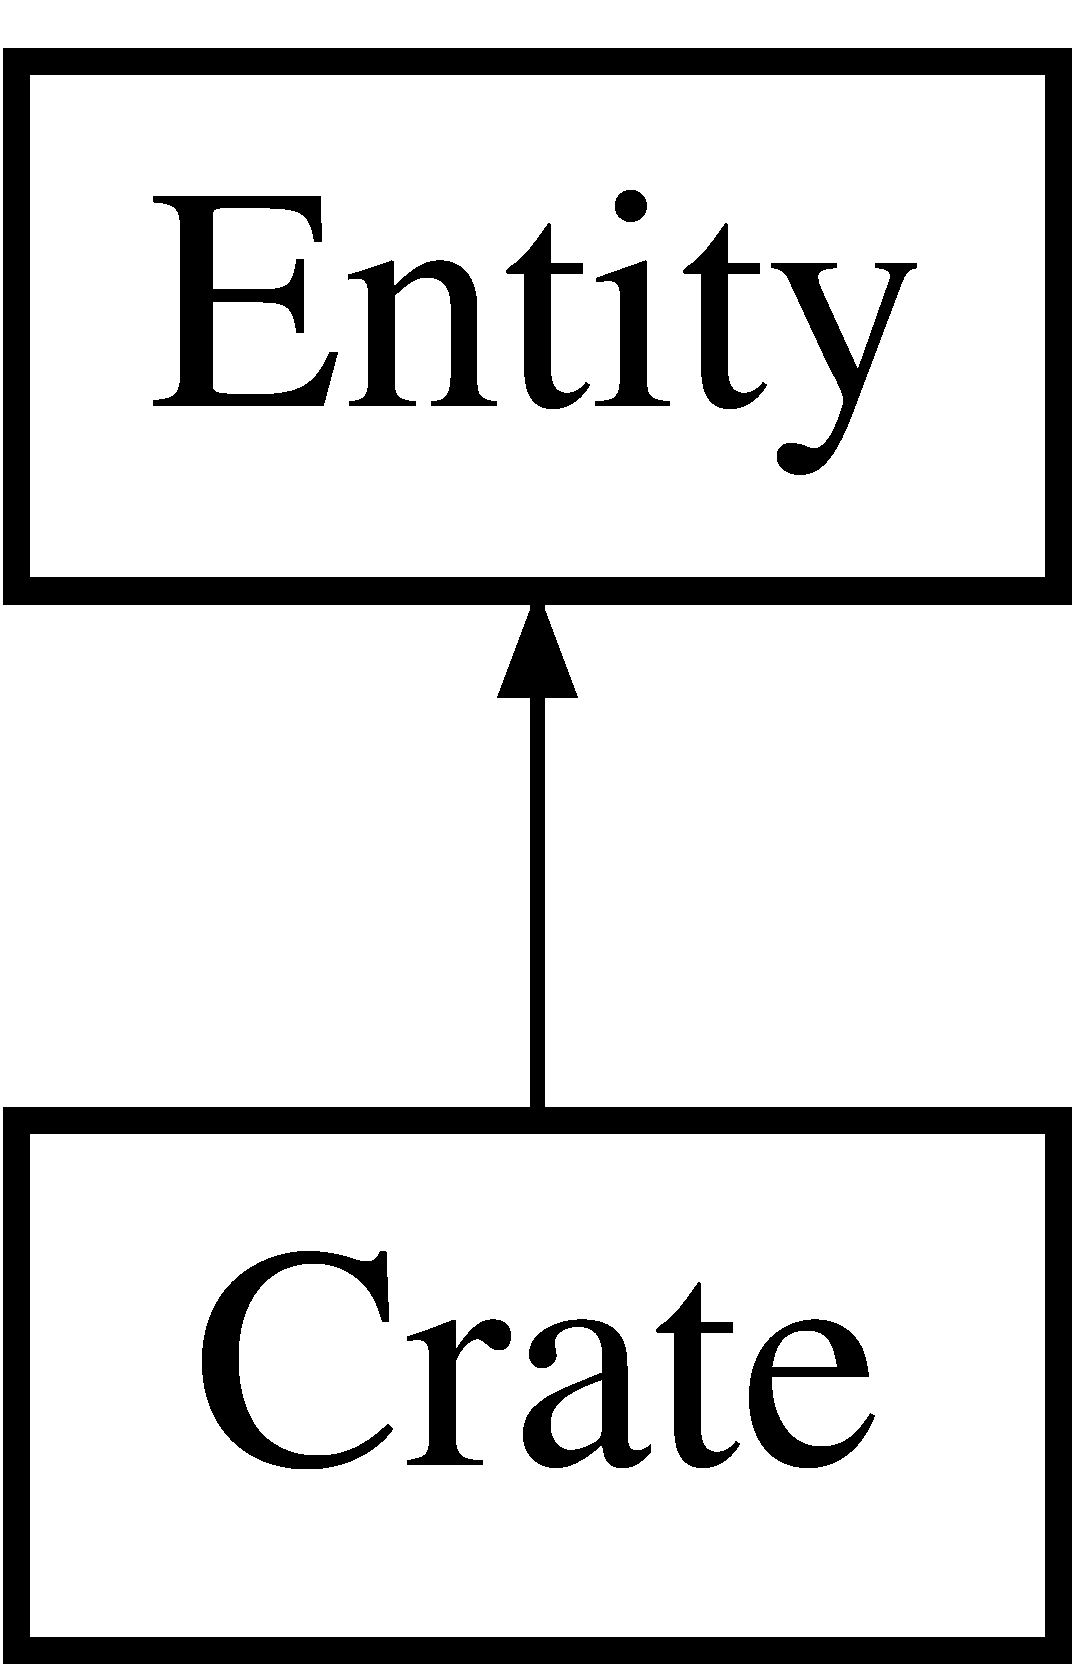
\includegraphics[height=2.000000cm]{class_crate}
\end{center}
\end{figure}
\subsection*{Public Member Functions}
\begin{DoxyCompactItemize}
\item 
\hyperlink{class_crate_aafcc7d0b42c7b58c3cb8afcb7d72d270}{Crate} (Vector2f \hyperlink{class_entity_a6af9d6498134ad0906011778bc5736db}{position}, Vector2f \hyperlink{class_entity_ae9a0a364c85f91ade5088b3610131417}{size}, bool \hyperlink{class_entity_af1b0754c9d5f4afa73834b23c6437101}{is\+Solid}=true, int \hyperlink{class_entity_a4edd9cc2506add0d9e27fade0bf957e8}{state}=states\+::normal)
\item 
\hyperlink{class_entity}{Entity} $\ast$ \hyperlink{class_crate_a6e4a24b12c92e8576c107b60f0b8f1a8}{hit} () override
\item 
void \hyperlink{class_crate_a2e9e544f1286c7de8830a8c2e7a955e9}{draw} (Render\+Window \&w) override
\end{DoxyCompactItemize}
\subsection*{Additional Inherited Members}


\subsection{Detailed Description}
\hyperlink{class_crate}{Crate} class Contains the crate graphic and overrides the necessary functions from \hyperlink{class_entity}{Entity}. 

Definition at line 14 of file Crate.\+h.



\subsection{Constructor \& Destructor Documentation}
\mbox{\Hypertarget{class_crate_aafcc7d0b42c7b58c3cb8afcb7d72d270}\label{class_crate_aafcc7d0b42c7b58c3cb8afcb7d72d270}} 
\index{Crate@{Crate}!Crate@{Crate}}
\index{Crate@{Crate}!Crate@{Crate}}
\subsubsection{\texorpdfstring{Crate()}{Crate()}}
{\footnotesize\ttfamily Crate\+::\+Crate (\begin{DoxyParamCaption}\item[{Vector2f}]{position,  }\item[{Vector2f}]{size,  }\item[{bool}]{is\+Solid = {\ttfamily true},  }\item[{int}]{state = {\ttfamily states\+:\+:normal} }\end{DoxyParamCaption})}



Definition at line 5 of file Crate.\+cpp.



\subsection{Member Function Documentation}
\mbox{\Hypertarget{class_crate_a2e9e544f1286c7de8830a8c2e7a955e9}\label{class_crate_a2e9e544f1286c7de8830a8c2e7a955e9}} 
\index{Crate@{Crate}!draw@{draw}}
\index{draw@{draw}!Crate@{Crate}}
\subsubsection{\texorpdfstring{draw()}{draw()}}
{\footnotesize\ttfamily void Crate\+::draw (\begin{DoxyParamCaption}\item[{Render\+Window \&}]{w }\end{DoxyParamCaption})\hspace{0.3cm}{\ttfamily [override]}, {\ttfamily [virtual]}}



Reimplemented from \hyperlink{class_entity_a030c3aa6641df7981a2d8a3fba890ec7}{Entity}.



Definition at line 21 of file Crate.\+cpp.

\mbox{\Hypertarget{class_crate_a6e4a24b12c92e8576c107b60f0b8f1a8}\label{class_crate_a6e4a24b12c92e8576c107b60f0b8f1a8}} 
\index{Crate@{Crate}!hit@{hit}}
\index{hit@{hit}!Crate@{Crate}}
\subsubsection{\texorpdfstring{hit()}{hit()}}
{\footnotesize\ttfamily \hyperlink{class_entity}{Entity} $\ast$ Crate\+::hit (\begin{DoxyParamCaption}{ }\end{DoxyParamCaption})\hspace{0.3cm}{\ttfamily [override]}, {\ttfamily [virtual]}}



Reimplemented from \hyperlink{class_entity_a29117f3f40e7069d5d4c1b2fca7819d6}{Entity}.



Definition at line 13 of file Crate.\+cpp.



The documentation for this class was generated from the following files\+:\begin{DoxyCompactItemize}
\item 
C\+:/\+Users/joost/\+Documents/\+Git\+Hub/topdown/\+Code/\+Team\+Topdown/\+Team\+Topdown/\hyperlink{_crate_8h}{Crate.\+h}\item 
C\+:/\+Users/joost/\+Documents/\+Git\+Hub/topdown/\+Code/\+Team\+Topdown/\+Team\+Topdown/\hyperlink{_crate_8cpp}{Crate.\+cpp}\end{DoxyCompactItemize}

\hypertarget{class_credits_state}{}\section{Credits\+State Class Reference}
\label{class_credits_state}\index{Credits\+State@{Credits\+State}}


The gamestate that shows the credits screen.  




{\ttfamily \#include $<$Credits\+State.\+hpp$>$}

Inheritance diagram for Credits\+State\+:\begin{figure}[H]
\begin{center}
\leavevmode
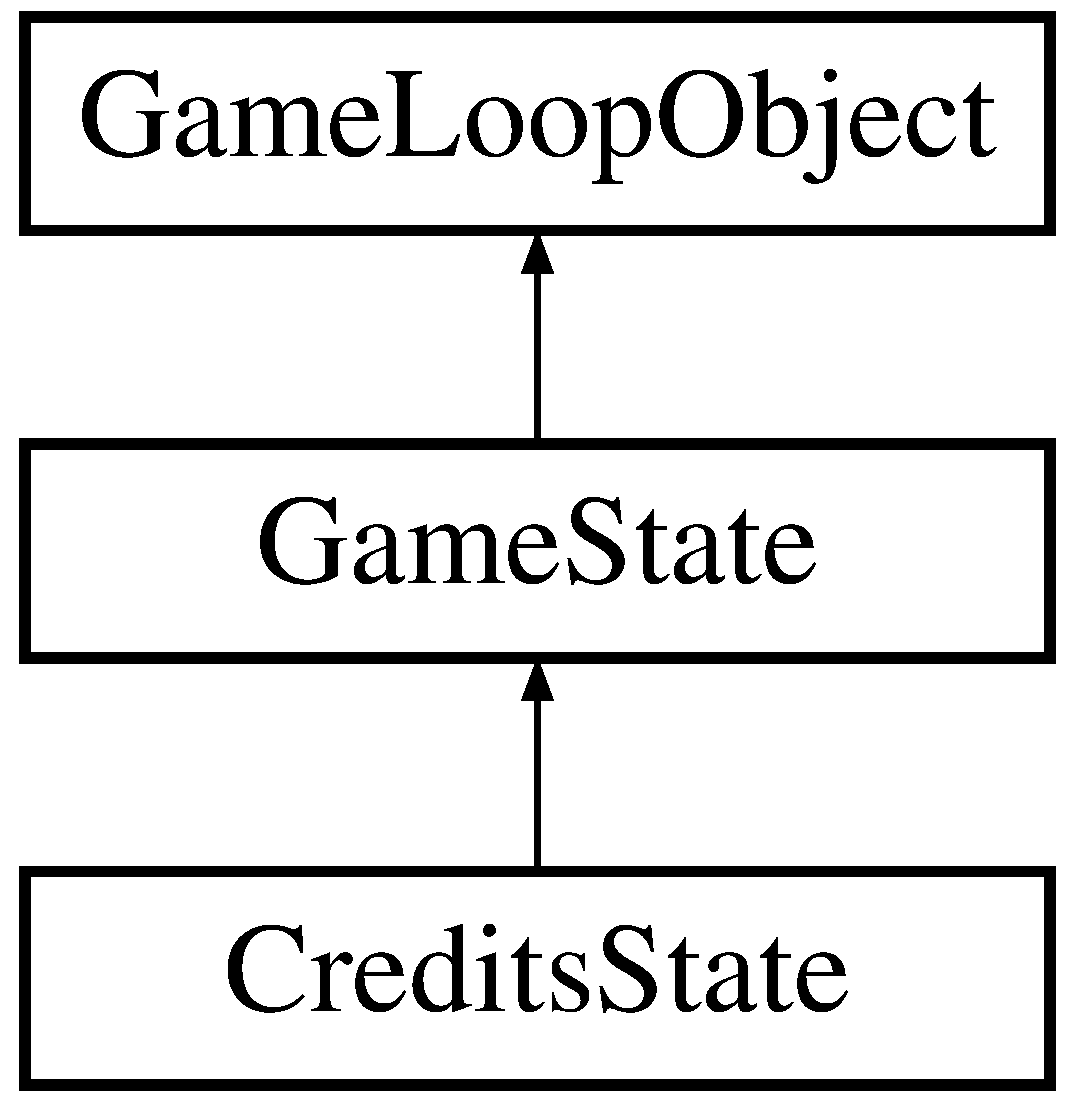
\includegraphics[height=3.000000cm]{class_credits_state}
\end{center}
\end{figure}
\subsection*{Public Member Functions}
\begin{DoxyCompactItemize}
\item 
\hyperlink{class_credits_state_a95163ef799a4afe3688d88e7cc8ae3b3}{Credits\+State} (sf\+::\+Render\+Window \&window, \hyperlink{class_game_state_manager}{Game\+State\+Manager} \&gsm, \hyperlink{struct_controls_input}{Controls\+Input} \&ci)
\begin{DoxyCompactList}\small\item\em The credits screen\textquotesingle{}s constructor method. \end{DoxyCompactList}\item 
void \hyperlink{class_credits_state_a63557b2290a2febb88e78ae90754a7ec}{Handle\+Input} ()
\begin{DoxyCompactList}\small\item\em The credits screen\textquotesingle{}s game loop method for handling user input. \end{DoxyCompactList}\item 
void \hyperlink{class_credits_state_a565adc4ac454f23941c5db684da56ad7}{Update} ()
\begin{DoxyCompactList}\small\item\em The credits screen\textquotesingle{}s game loop method for updating the game. \end{DoxyCompactList}\item 
void \hyperlink{class_credits_state_a085e7decf7f1fc7edae68db50851b84a}{Draw} (sf\+::\+Render\+Window \&window)
\begin{DoxyCompactList}\small\item\em The credits screen\textquotesingle{}s game loop method for drawing on the window. \end{DoxyCompactList}\item 
void \hyperlink{class_credits_state_ad87636e8b9438092bd0151185f385c17}{Reset} ()
\begin{DoxyCompactList}\small\item\em The credits state\textquotesingle{}s reset method to reset all values to default. \end{DoxyCompactList}\end{DoxyCompactItemize}


\subsection{Detailed Description}
The gamestate that shows the credits screen. 

This game shows the credits screen. Pressing space/enter/backspace lets the player return to the main menu. 

Definition at line 15 of file Credits\+State.\+hpp.



\subsection{Constructor \& Destructor Documentation}
\mbox{\Hypertarget{class_credits_state_a95163ef799a4afe3688d88e7cc8ae3b3}\label{class_credits_state_a95163ef799a4afe3688d88e7cc8ae3b3}} 
\index{Credits\+State@{Credits\+State}!Credits\+State@{Credits\+State}}
\index{Credits\+State@{Credits\+State}!Credits\+State@{Credits\+State}}
\subsubsection{\texorpdfstring{Credits\+State()}{CreditsState()}}
{\footnotesize\ttfamily Credits\+State\+::\+Credits\+State (\begin{DoxyParamCaption}\item[{sf\+::\+Render\+Window \&}]{window,  }\item[{\hyperlink{class_game_state_manager}{Game\+State\+Manager} \&}]{gsm,  }\item[{\hyperlink{struct_controls_input}{Controls\+Input} \&}]{ci }\end{DoxyParamCaption})}



The credits screen\textquotesingle{}s constructor method. 

The credits screen\textquotesingle{}s constructor requires a window to draw on, the gamestatemanager to be able to switch states and the controlsinput to read user input. 

Definition at line 5 of file Credits\+State.\+cpp.



\subsection{Member Function Documentation}
\mbox{\Hypertarget{class_credits_state_a085e7decf7f1fc7edae68db50851b84a}\label{class_credits_state_a085e7decf7f1fc7edae68db50851b84a}} 
\index{Credits\+State@{Credits\+State}!Draw@{Draw}}
\index{Draw@{Draw}!Credits\+State@{Credits\+State}}
\subsubsection{\texorpdfstring{Draw()}{Draw()}}
{\footnotesize\ttfamily void Credits\+State\+::\+Draw (\begin{DoxyParamCaption}\item[{sf\+::\+Render\+Window \&}]{window }\end{DoxyParamCaption})\hspace{0.3cm}{\ttfamily [virtual]}}



The credits screen\textquotesingle{}s game loop method for drawing on the window. 

Draws the background and text on the screen. 

Reimplemented from \hyperlink{class_game_state_a8741c5c696c6c366beb4b845c08c3cf8}{Game\+State}.



Definition at line 35 of file Credits\+State.\+cpp.

\mbox{\Hypertarget{class_credits_state_a63557b2290a2febb88e78ae90754a7ec}\label{class_credits_state_a63557b2290a2febb88e78ae90754a7ec}} 
\index{Credits\+State@{Credits\+State}!Handle\+Input@{Handle\+Input}}
\index{Handle\+Input@{Handle\+Input}!Credits\+State@{Credits\+State}}
\subsubsection{\texorpdfstring{Handle\+Input()}{HandleInput()}}
{\footnotesize\ttfamily void Credits\+State\+::\+Handle\+Input (\begin{DoxyParamCaption}{ }\end{DoxyParamCaption})\hspace{0.3cm}{\ttfamily [virtual]}}



The credits screen\textquotesingle{}s game loop method for handling user input. 

This method handles all user input related to this gamestate. Pressing space/enter/backspace lets the player return to the main menu. 

Reimplemented from \hyperlink{class_game_state_a8bce2828cee99ae7c07322804531fd01}{Game\+State}.



Definition at line 22 of file Credits\+State.\+cpp.

\mbox{\Hypertarget{class_credits_state_ad87636e8b9438092bd0151185f385c17}\label{class_credits_state_ad87636e8b9438092bd0151185f385c17}} 
\index{Credits\+State@{Credits\+State}!Reset@{Reset}}
\index{Reset@{Reset}!Credits\+State@{Credits\+State}}
\subsubsection{\texorpdfstring{Reset()}{Reset()}}
{\footnotesize\ttfamily void Credits\+State\+::\+Reset (\begin{DoxyParamCaption}{ }\end{DoxyParamCaption})\hspace{0.3cm}{\ttfamily [virtual]}}



The credits state\textquotesingle{}s reset method to reset all values to default. 

Doesn\textquotesingle{}t do anything. 

Reimplemented from \hyperlink{class_game_state_a46ac6317883dff0eba4f8f305af6b6bb}{Game\+State}.



Definition at line 44 of file Credits\+State.\+cpp.

\mbox{\Hypertarget{class_credits_state_a565adc4ac454f23941c5db684da56ad7}\label{class_credits_state_a565adc4ac454f23941c5db684da56ad7}} 
\index{Credits\+State@{Credits\+State}!Update@{Update}}
\index{Update@{Update}!Credits\+State@{Credits\+State}}
\subsubsection{\texorpdfstring{Update()}{Update()}}
{\footnotesize\ttfamily void Credits\+State\+::\+Update (\begin{DoxyParamCaption}{ }\end{DoxyParamCaption})\hspace{0.3cm}{\ttfamily [virtual]}}



The credits screen\textquotesingle{}s game loop method for updating the game. 

Currently only checks if a gamestate switch should be executed. 

Reimplemented from \hyperlink{class_game_state_a5be51b634f95bc6e57066ad6931aa18b}{Game\+State}.



Definition at line 30 of file Credits\+State.\+cpp.



The documentation for this class was generated from the following files\+:\begin{DoxyCompactItemize}
\item 
C\+:/\+Users/joost/\+Documents/\+Git\+Hub/topdown/\+Code/\+Team\+Topdown/\+Team\+Topdown/\hyperlink{_credits_state_8hpp}{Credits\+State.\+hpp}\item 
C\+:/\+Users/joost/\+Documents/\+Git\+Hub/topdown/\+Code/\+Team\+Topdown/\+Team\+Topdown/\hyperlink{_credits_state_8cpp}{Credits\+State.\+cpp}\end{DoxyCompactItemize}

\hypertarget{class_cursor}{}\section{Cursor Class Reference}
\label{class_cursor}\index{Cursor@{Cursor}}


Class for the \hyperlink{class_cursor}{Cursor} entity. Overrides the needed functions from \hyperlink{class_entity}{Entity}. Places a sprite on the cursor location.  




{\ttfamily \#include $<$Cursor.\+h$>$}

Inheritance diagram for Cursor\+:\begin{figure}[H]
\begin{center}
\leavevmode
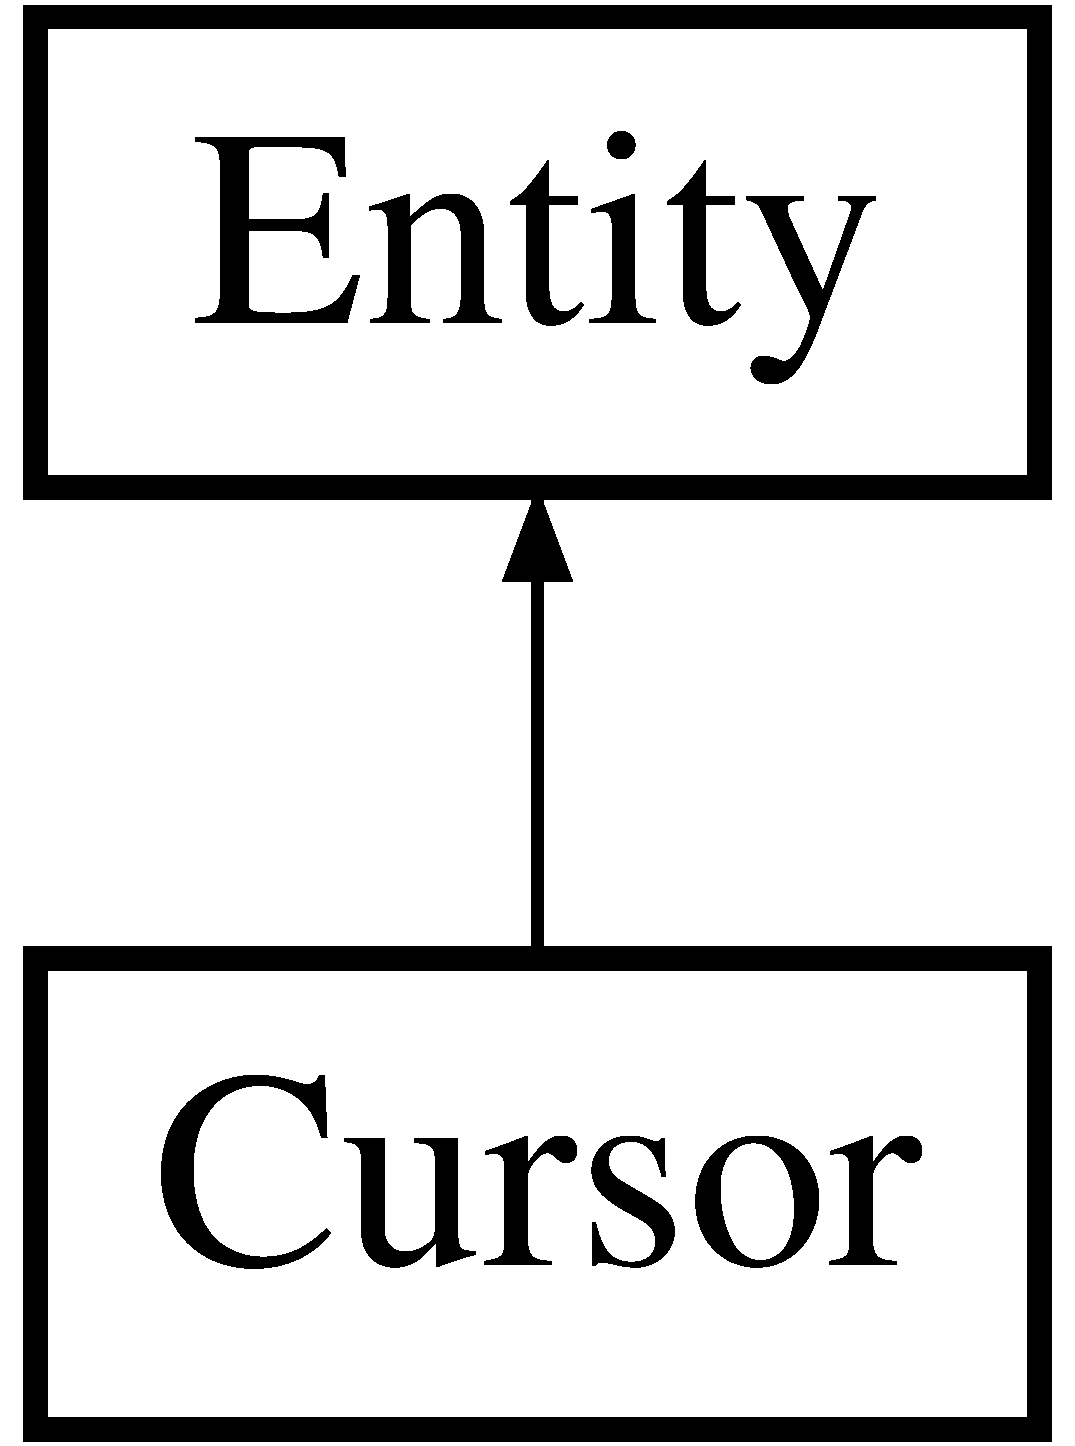
\includegraphics[height=2.000000cm]{class_cursor}
\end{center}
\end{figure}
\subsection*{Public Member Functions}
\begin{DoxyCompactItemize}
\item 
\hyperlink{class_cursor_ac1cd6075c59b1fd16bf87bb9a366cca9}{Cursor} (sf\+::\+Render\+Window \&window, Vector2f \hyperlink{class_entity_a6af9d6498134ad0906011778bc5736db}{position}, Vector2f \hyperlink{class_entity_ae9a0a364c85f91ade5088b3610131417}{size}, \hyperlink{struct_controls_input}{Controls\+Input} \&\hyperlink{classcontrols_input}{controls\+Input}, bool \hyperlink{class_entity_af1b0754c9d5f4afa73834b23c6437101}{is\+Solid})
\item 
void \hyperlink{class_cursor_a2450501ae27244acb089209436d5b112}{update} () override
\item 
void \hyperlink{class_cursor_a31c09a077d14237953223980197fdd17}{draw} (Render\+Window \&w) override
\item 
Vector2f \hyperlink{class_cursor_a214e135fad5e686f5bcfea34806c8730}{get\+Pos} ()
\end{DoxyCompactItemize}
\subsection*{Additional Inherited Members}


\subsection{Detailed Description}
Class for the \hyperlink{class_cursor}{Cursor} entity. Overrides the needed functions from \hyperlink{class_entity}{Entity}. Places a sprite on the cursor location. 

Definition at line 15 of file Cursor.\+h.



\subsection{Constructor \& Destructor Documentation}
\mbox{\Hypertarget{class_cursor_ac1cd6075c59b1fd16bf87bb9a366cca9}\label{class_cursor_ac1cd6075c59b1fd16bf87bb9a366cca9}} 
\index{Cursor@{Cursor}!Cursor@{Cursor}}
\index{Cursor@{Cursor}!Cursor@{Cursor}}
\subsubsection{\texorpdfstring{Cursor()}{Cursor()}}
{\footnotesize\ttfamily Cursor\+::\+Cursor (\begin{DoxyParamCaption}\item[{sf\+::\+Render\+Window \&}]{window,  }\item[{Vector2f}]{position,  }\item[{Vector2f}]{size,  }\item[{\hyperlink{struct_controls_input}{Controls\+Input} \&}]{controls\+Input,  }\item[{bool}]{is\+Solid }\end{DoxyParamCaption})}



Definition at line 4 of file Cursor.\+cpp.



\subsection{Member Function Documentation}
\mbox{\Hypertarget{class_cursor_a31c09a077d14237953223980197fdd17}\label{class_cursor_a31c09a077d14237953223980197fdd17}} 
\index{Cursor@{Cursor}!draw@{draw}}
\index{draw@{draw}!Cursor@{Cursor}}
\subsubsection{\texorpdfstring{draw()}{draw()}}
{\footnotesize\ttfamily void Cursor\+::draw (\begin{DoxyParamCaption}\item[{Render\+Window \&}]{w }\end{DoxyParamCaption})\hspace{0.3cm}{\ttfamily [override]}, {\ttfamily [virtual]}}

/void \hyperlink{class_cursor_a31c09a077d14237953223980197fdd17}{draw()} /brief draws certain graphics within this class
\begin{DoxyItemize}
\item draws the cursor sprite 
\end{DoxyItemize}

Reimplemented from \hyperlink{class_entity_a030c3aa6641df7981a2d8a3fba890ec7}{Entity}.



Definition at line 18 of file Cursor.\+cpp.

\mbox{\Hypertarget{class_cursor_a214e135fad5e686f5bcfea34806c8730}\label{class_cursor_a214e135fad5e686f5bcfea34806c8730}} 
\index{Cursor@{Cursor}!get\+Pos@{get\+Pos}}
\index{get\+Pos@{get\+Pos}!Cursor@{Cursor}}
\subsubsection{\texorpdfstring{get\+Pos()}{getPos()}}
{\footnotesize\ttfamily Vector2f Cursor\+::get\+Pos (\begin{DoxyParamCaption}{ }\end{DoxyParamCaption})\hspace{0.3cm}{\ttfamily [virtual]}}

/\+Vector2f \hyperlink{class_cursor_a214e135fad5e686f5bcfea34806c8730}{get\+Pos()} /brief returns the position of the cursor 

Reimplemented from \hyperlink{class_entity_a8b6080f0ab76702fcd00108aef8ea9dd}{Entity}.



Definition at line 23 of file Cursor.\+cpp.

\mbox{\Hypertarget{class_cursor_a2450501ae27244acb089209436d5b112}\label{class_cursor_a2450501ae27244acb089209436d5b112}} 
\index{Cursor@{Cursor}!update@{update}}
\index{update@{update}!Cursor@{Cursor}}
\subsubsection{\texorpdfstring{update()}{update()}}
{\footnotesize\ttfamily void Cursor\+::update (\begin{DoxyParamCaption}{ }\end{DoxyParamCaption})\hspace{0.3cm}{\ttfamily [override]}, {\ttfamily [virtual]}}

/void \hyperlink{class_cursor_a2450501ae27244acb089209436d5b112}{update()} /brief updates the data within this class
\begin{DoxyItemize}
\item updates the cursor sprite location 
\end{DoxyItemize}

Reimplemented from \hyperlink{class_entity_aed73e98b980b85833428c935cc1c69f8}{Entity}.



Definition at line 13 of file Cursor.\+cpp.



The documentation for this class was generated from the following files\+:\begin{DoxyCompactItemize}
\item 
C\+:/\+Users/joost/\+Documents/\+Git\+Hub/topdown/\+Code/\+Team\+Topdown/\+Team\+Topdown/\hyperlink{_cursor_8h}{Cursor.\+h}\item 
C\+:/\+Users/joost/\+Documents/\+Git\+Hub/topdown/\+Code/\+Team\+Topdown/\+Team\+Topdown/\hyperlink{_cursor_8cpp}{Cursor.\+cpp}\end{DoxyCompactItemize}

\hypertarget{class_enemy}{}\section{Enemy Class Reference}
\label{class_enemy}\index{Enemy@{Enemy}}


Handles enemy movement, interaction and art. The enemy class creates an instance of an enemy and adds the position given as waypoint. If other waypoints are added, which are first in line, we set entity position to that waypoint. Once all waypoints are added (map is looped through entirely) we create a queue from this map of waypoints. If we only have 1 waypoint we empty our queue and stand still. If we have an even amount, we loop through those points. If the amount of waypoints is uneven, we create a line instead.  




{\ttfamily \#include $<$Enemy.\+h$>$}

Inheritance diagram for Enemy\+:\begin{figure}[H]
\begin{center}
\leavevmode
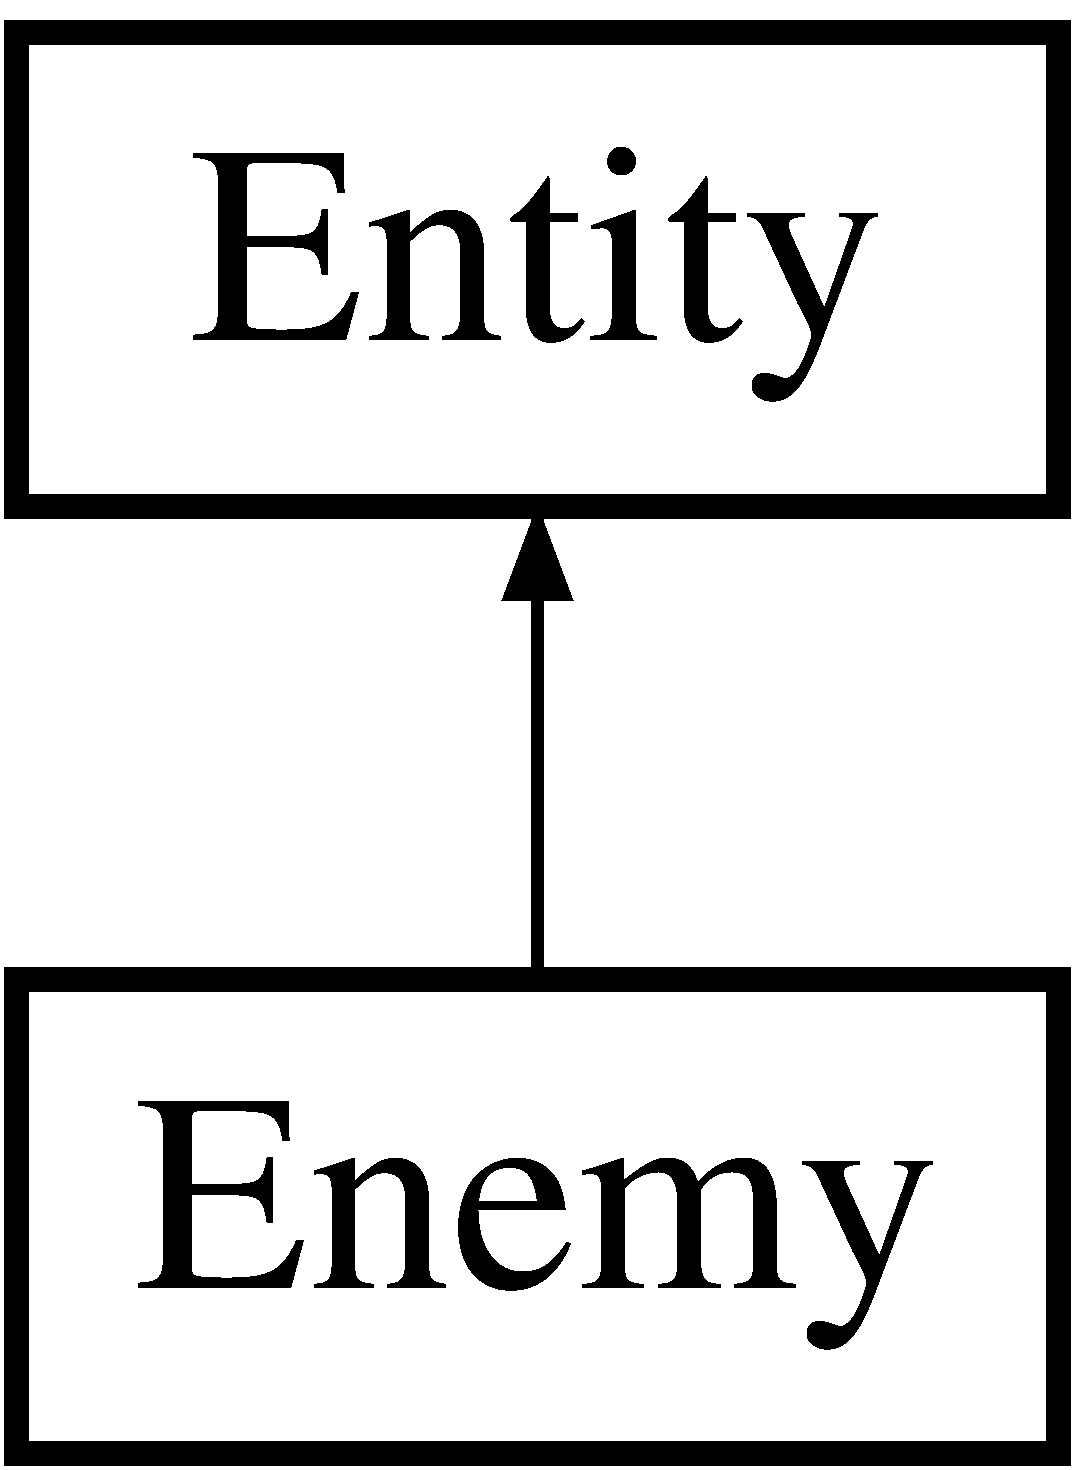
\includegraphics[height=2.000000cm]{class_enemy}
\end{center}
\end{figure}
\subsection*{Public Member Functions}
\begin{DoxyCompactItemize}
\item 
\hyperlink{class_enemy_aa606fada257eefe1469e462768285dff}{Enemy} (Vector2f \hyperlink{class_entity_a6af9d6498134ad0906011778bc5736db}{position}, unsigned int waypoint\+Nr, Vector2f \hyperlink{class_entity_ae9a0a364c85f91ade5088b3610131417}{size}=Vector2f(24.\+0f, 24.\+0f), bool is\+Solid=true, int state=states\+::patrolling, bool hostile=false, Vector2f \&player\+Pos=\+Vector2f(0, 0), Vector2f init\+Look\+At\+Obj=\+Vector2f(0, 0))
\item 
void \hyperlink{class_enemy_a5b54ac52247fc27b4860c04e8f1464d9}{add\+Waypoint} (Vector2f \hyperlink{class_entity_a6af9d6498134ad0906011778bc5736db}{position}, unsigned int number)
\item 
void \hyperlink{class_enemy_a9c48b3be7c2ebbb7dce8b45183299895}{create\+Waypoint\+Queue} ()
\item 
void \hyperlink{class_enemy_aa89bba7f1bb9f16c9cee861137968c30}{rotate} ()
\item 
void \hyperlink{class_enemy_aefbc9a7b2370957331e608932c458b52}{move\+Towards} (Vector2f direction)
\item 
\hyperlink{class_entity}{Entity} $\ast$ \hyperlink{class_enemy_a6cb8f8dbec88de9b2e95643709e349a3}{hit} () override
\item 
void \hyperlink{class_enemy_aa70d742da02995011f1618acc9e303db}{update} () override
\item 
void \hyperlink{class_enemy_a582d09158d692070f4becf68220bf6b6}{draw} (Render\+Window \&window) override
\item 
Vector2f \hyperlink{class_enemy_a65af045027f5fd7396b420f0d4c34dac}{get\+Pos} ()
\item 
Vector2f \hyperlink{class_enemy_aa55a89207573ebad16ba1556b105d692}{get\+Look\+At\+Obj} ()
\item 
bool \hyperlink{class_enemy_aa50adebfe1bd8b83a6a0571f3635c932}{collides\+With} (\hyperlink{class_entity}{Entity} $\ast$other)
\end{DoxyCompactItemize}
\subsection*{Public Attributes}
\begin{DoxyCompactItemize}
\item 
std\+::queue$<$ Vector2f $>$ \hyperlink{class_enemy_a0265035a86653dde11df05cd8f0ceaa5}{waypoints}
\item 
float \hyperlink{class_enemy_af0b960378e5235ef1e46a4ecdd85674d}{rotation}
\end{DoxyCompactItemize}
\subsection*{Additional Inherited Members}


\subsection{Detailed Description}
Handles enemy movement, interaction and art. The enemy class creates an instance of an enemy and adds the position given as waypoint. If other waypoints are added, which are first in line, we set entity position to that waypoint. Once all waypoints are added (map is looped through entirely) we create a queue from this map of waypoints. If we only have 1 waypoint we empty our queue and stand still. If we have an even amount, we loop through those points. If the amount of waypoints is uneven, we create a line instead. 

Definition at line 25 of file Enemy.\+h.



\subsection{Constructor \& Destructor Documentation}
\mbox{\Hypertarget{class_enemy_aa606fada257eefe1469e462768285dff}\label{class_enemy_aa606fada257eefe1469e462768285dff}} 
\index{Enemy@{Enemy}!Enemy@{Enemy}}
\index{Enemy@{Enemy}!Enemy@{Enemy}}
\subsubsection{\texorpdfstring{Enemy()}{Enemy()}}
{\footnotesize\ttfamily Enemy\+::\+Enemy (\begin{DoxyParamCaption}\item[{Vector2f}]{position,  }\item[{unsigned int}]{waypoint\+Nr,  }\item[{Vector2f}]{size = {\ttfamily Vector2f(24.0f,~24.0f)},  }\item[{bool}]{is\+Solid = {\ttfamily true},  }\item[{int}]{state = {\ttfamily states\+:\+:patrolling},  }\item[{bool}]{hostile = {\ttfamily false},  }\item[{Vector2f \&}]{player\+Pos = {\ttfamily Vector2f(0,0)},  }\item[{Vector2f}]{init\+Look\+At\+Obj = {\ttfamily Vector2f(0,0)} }\end{DoxyParamCaption})}



Definition at line 5 of file Enemy.\+cpp.



\subsection{Member Function Documentation}
\mbox{\Hypertarget{class_enemy_a5b54ac52247fc27b4860c04e8f1464d9}\label{class_enemy_a5b54ac52247fc27b4860c04e8f1464d9}} 
\index{Enemy@{Enemy}!add\+Waypoint@{add\+Waypoint}}
\index{add\+Waypoint@{add\+Waypoint}!Enemy@{Enemy}}
\subsubsection{\texorpdfstring{add\+Waypoint()}{addWaypoint()}}
{\footnotesize\ttfamily void Enemy\+::add\+Waypoint (\begin{DoxyParamCaption}\item[{Vector2f}]{position,  }\item[{unsigned int}]{number }\end{DoxyParamCaption})}



Definition at line 17 of file Enemy.\+cpp.

\mbox{\Hypertarget{class_enemy_aa50adebfe1bd8b83a6a0571f3635c932}\label{class_enemy_aa50adebfe1bd8b83a6a0571f3635c932}} 
\index{Enemy@{Enemy}!collides\+With@{collides\+With}}
\index{collides\+With@{collides\+With}!Enemy@{Enemy}}
\subsubsection{\texorpdfstring{collides\+With()}{collidesWith()}}
{\footnotesize\ttfamily bool Enemy\+::collides\+With (\begin{DoxyParamCaption}\item[{\hyperlink{class_entity}{Entity} $\ast$}]{other }\end{DoxyParamCaption})}

/bool \hyperlink{class_enemy_aa50adebfe1bd8b83a6a0571f3635c932}{collides\+With(\+Entity$\ast$ other)} /brief returns boolean if enemy is colliding with another entity 

Definition at line 107 of file Enemy.\+cpp.

\mbox{\Hypertarget{class_enemy_a9c48b3be7c2ebbb7dce8b45183299895}\label{class_enemy_a9c48b3be7c2ebbb7dce8b45183299895}} 
\index{Enemy@{Enemy}!create\+Waypoint\+Queue@{create\+Waypoint\+Queue}}
\index{create\+Waypoint\+Queue@{create\+Waypoint\+Queue}!Enemy@{Enemy}}
\subsubsection{\texorpdfstring{create\+Waypoint\+Queue()}{createWaypointQueue()}}
{\footnotesize\ttfamily void Enemy\+::create\+Waypoint\+Queue (\begin{DoxyParamCaption}{ }\end{DoxyParamCaption})}

/void \hyperlink{class_enemy_a9c48b3be7c2ebbb7dce8b45183299895}{create\+Waypoint\+Queue()} /brief creates a que of waypoints for the enemy to follow 

Definition at line 22 of file Enemy.\+cpp.

\mbox{\Hypertarget{class_enemy_a582d09158d692070f4becf68220bf6b6}\label{class_enemy_a582d09158d692070f4becf68220bf6b6}} 
\index{Enemy@{Enemy}!draw@{draw}}
\index{draw@{draw}!Enemy@{Enemy}}
\subsubsection{\texorpdfstring{draw()}{draw()}}
{\footnotesize\ttfamily void Enemy\+::draw (\begin{DoxyParamCaption}\item[{Render\+Window \&}]{window }\end{DoxyParamCaption})\hspace{0.3cm}{\ttfamily [override]}, {\ttfamily [virtual]}}



Reimplemented from \hyperlink{class_entity_a030c3aa6641df7981a2d8a3fba890ec7}{Entity}.



Definition at line 92 of file Enemy.\+cpp.

\mbox{\Hypertarget{class_enemy_aa55a89207573ebad16ba1556b105d692}\label{class_enemy_aa55a89207573ebad16ba1556b105d692}} 
\index{Enemy@{Enemy}!get\+Look\+At\+Obj@{get\+Look\+At\+Obj}}
\index{get\+Look\+At\+Obj@{get\+Look\+At\+Obj}!Enemy@{Enemy}}
\subsubsection{\texorpdfstring{get\+Look\+At\+Obj()}{getLookAtObj()}}
{\footnotesize\ttfamily Vector2f Enemy\+::get\+Look\+At\+Obj (\begin{DoxyParamCaption}{ }\end{DoxyParamCaption})}



Definition at line 102 of file Enemy.\+cpp.

\mbox{\Hypertarget{class_enemy_a65af045027f5fd7396b420f0d4c34dac}\label{class_enemy_a65af045027f5fd7396b420f0d4c34dac}} 
\index{Enemy@{Enemy}!get\+Pos@{get\+Pos}}
\index{get\+Pos@{get\+Pos}!Enemy@{Enemy}}
\subsubsection{\texorpdfstring{get\+Pos()}{getPos()}}
{\footnotesize\ttfamily Vector2f Enemy\+::get\+Pos (\begin{DoxyParamCaption}{ }\end{DoxyParamCaption})\hspace{0.3cm}{\ttfamily [virtual]}}



Reimplemented from \hyperlink{class_entity_a8b6080f0ab76702fcd00108aef8ea9dd}{Entity}.



Definition at line 97 of file Enemy.\+cpp.

\mbox{\Hypertarget{class_enemy_a6cb8f8dbec88de9b2e95643709e349a3}\label{class_enemy_a6cb8f8dbec88de9b2e95643709e349a3}} 
\index{Enemy@{Enemy}!hit@{hit}}
\index{hit@{hit}!Enemy@{Enemy}}
\subsubsection{\texorpdfstring{hit()}{hit()}}
{\footnotesize\ttfamily \hyperlink{class_entity}{Entity} $\ast$ Enemy\+::hit (\begin{DoxyParamCaption}{ }\end{DoxyParamCaption})\hspace{0.3cm}{\ttfamily [override]}, {\ttfamily [virtual]}}

/void Entity$\ast$ \hyperlink{class_enemy_a6cb8f8dbec88de9b2e95643709e349a3}{hit()} override /brief overrides the hit function from \hyperlink{class_entity}{Entity} /description This funciton will be called when the enemy should die. When called, the enemy switches to it\textquotesingle{}s dead state and the texture will be updated to visualise a dead enemy. \hyperlink{class_enemy}{Enemy} interactions will also be disabled. A random amount of bullets will be dropped for the player to pick up at the enemy\textquotesingle{}s locatoin. 

Reimplemented from \hyperlink{class_entity_a29117f3f40e7069d5d4c1b2fca7819d6}{Entity}.



Definition at line 44 of file Enemy.\+cpp.

\mbox{\Hypertarget{class_enemy_aefbc9a7b2370957331e608932c458b52}\label{class_enemy_aefbc9a7b2370957331e608932c458b52}} 
\index{Enemy@{Enemy}!move\+Towards@{move\+Towards}}
\index{move\+Towards@{move\+Towards}!Enemy@{Enemy}}
\subsubsection{\texorpdfstring{move\+Towards()}{moveTowards()}}
{\footnotesize\ttfamily void Enemy\+::move\+Towards (\begin{DoxyParamCaption}\item[{Vector2f}]{direction }\end{DoxyParamCaption})}



Definition at line 86 of file Enemy.\+cpp.

\mbox{\Hypertarget{class_enemy_aa89bba7f1bb9f16c9cee861137968c30}\label{class_enemy_aa89bba7f1bb9f16c9cee861137968c30}} 
\index{Enemy@{Enemy}!rotate@{rotate}}
\index{rotate@{rotate}!Enemy@{Enemy}}
\subsubsection{\texorpdfstring{rotate()}{rotate()}}
{\footnotesize\ttfamily void Enemy\+::rotate (\begin{DoxyParamCaption}{ }\end{DoxyParamCaption})}



Definition at line 79 of file Enemy.\+cpp.

\mbox{\Hypertarget{class_enemy_aa70d742da02995011f1618acc9e303db}\label{class_enemy_aa70d742da02995011f1618acc9e303db}} 
\index{Enemy@{Enemy}!update@{update}}
\index{update@{update}!Enemy@{Enemy}}
\subsubsection{\texorpdfstring{update()}{update()}}
{\footnotesize\ttfamily void Enemy\+::update (\begin{DoxyParamCaption}{ }\end{DoxyParamCaption})\hspace{0.3cm}{\ttfamily [override]}, {\ttfamily [virtual]}}

/void \hyperlink{class_enemy_aa70d742da02995011f1618acc9e303db}{update()} override; /brief overrides the update function from \hyperlink{class_entity}{Entity} /description This function controls the patrolling and alarmed state. When patrolling, the enemy will move to it\textquotesingle{}s next waypoint if not stationary. When alarmed, the enemy will track the players location. The position will be set at the end of the function. 

Reimplemented from \hyperlink{class_entity_aed73e98b980b85833428c935cc1c69f8}{Entity}.



Definition at line 57 of file Enemy.\+cpp.



\subsection{Member Data Documentation}
\mbox{\Hypertarget{class_enemy_af0b960378e5235ef1e46a4ecdd85674d}\label{class_enemy_af0b960378e5235ef1e46a4ecdd85674d}} 
\index{Enemy@{Enemy}!rotation@{rotation}}
\index{rotation@{rotation}!Enemy@{Enemy}}
\subsubsection{\texorpdfstring{rotation}{rotation}}
{\footnotesize\ttfamily float Enemy\+::rotation}



Definition at line 63 of file Enemy.\+h.

\mbox{\Hypertarget{class_enemy_a0265035a86653dde11df05cd8f0ceaa5}\label{class_enemy_a0265035a86653dde11df05cd8f0ceaa5}} 
\index{Enemy@{Enemy}!waypoints@{waypoints}}
\index{waypoints@{waypoints}!Enemy@{Enemy}}
\subsubsection{\texorpdfstring{waypoints}{waypoints}}
{\footnotesize\ttfamily std\+::queue$<$Vector2f$>$ Enemy\+::waypoints}



Definition at line 40 of file Enemy.\+h.



The documentation for this class was generated from the following files\+:\begin{DoxyCompactItemize}
\item 
C\+:/\+Users/joost/\+Documents/\+Git\+Hub/topdown/\+Code/\+Team\+Topdown/\+Team\+Topdown/\hyperlink{_enemy_8h}{Enemy.\+h}\item 
C\+:/\+Users/joost/\+Documents/\+Git\+Hub/topdown/\+Code/\+Team\+Topdown/\+Team\+Topdown/\hyperlink{_enemy_8cpp}{Enemy.\+cpp}\end{DoxyCompactItemize}

\hypertarget{class_entity}{}\section{Entity Class Reference}
\label{class_entity}\index{Entity@{Entity}}


{\ttfamily \#include $<$Entity.\+h$>$}

Inheritance diagram for Entity\+:\begin{figure}[H]
\begin{center}
\leavevmode
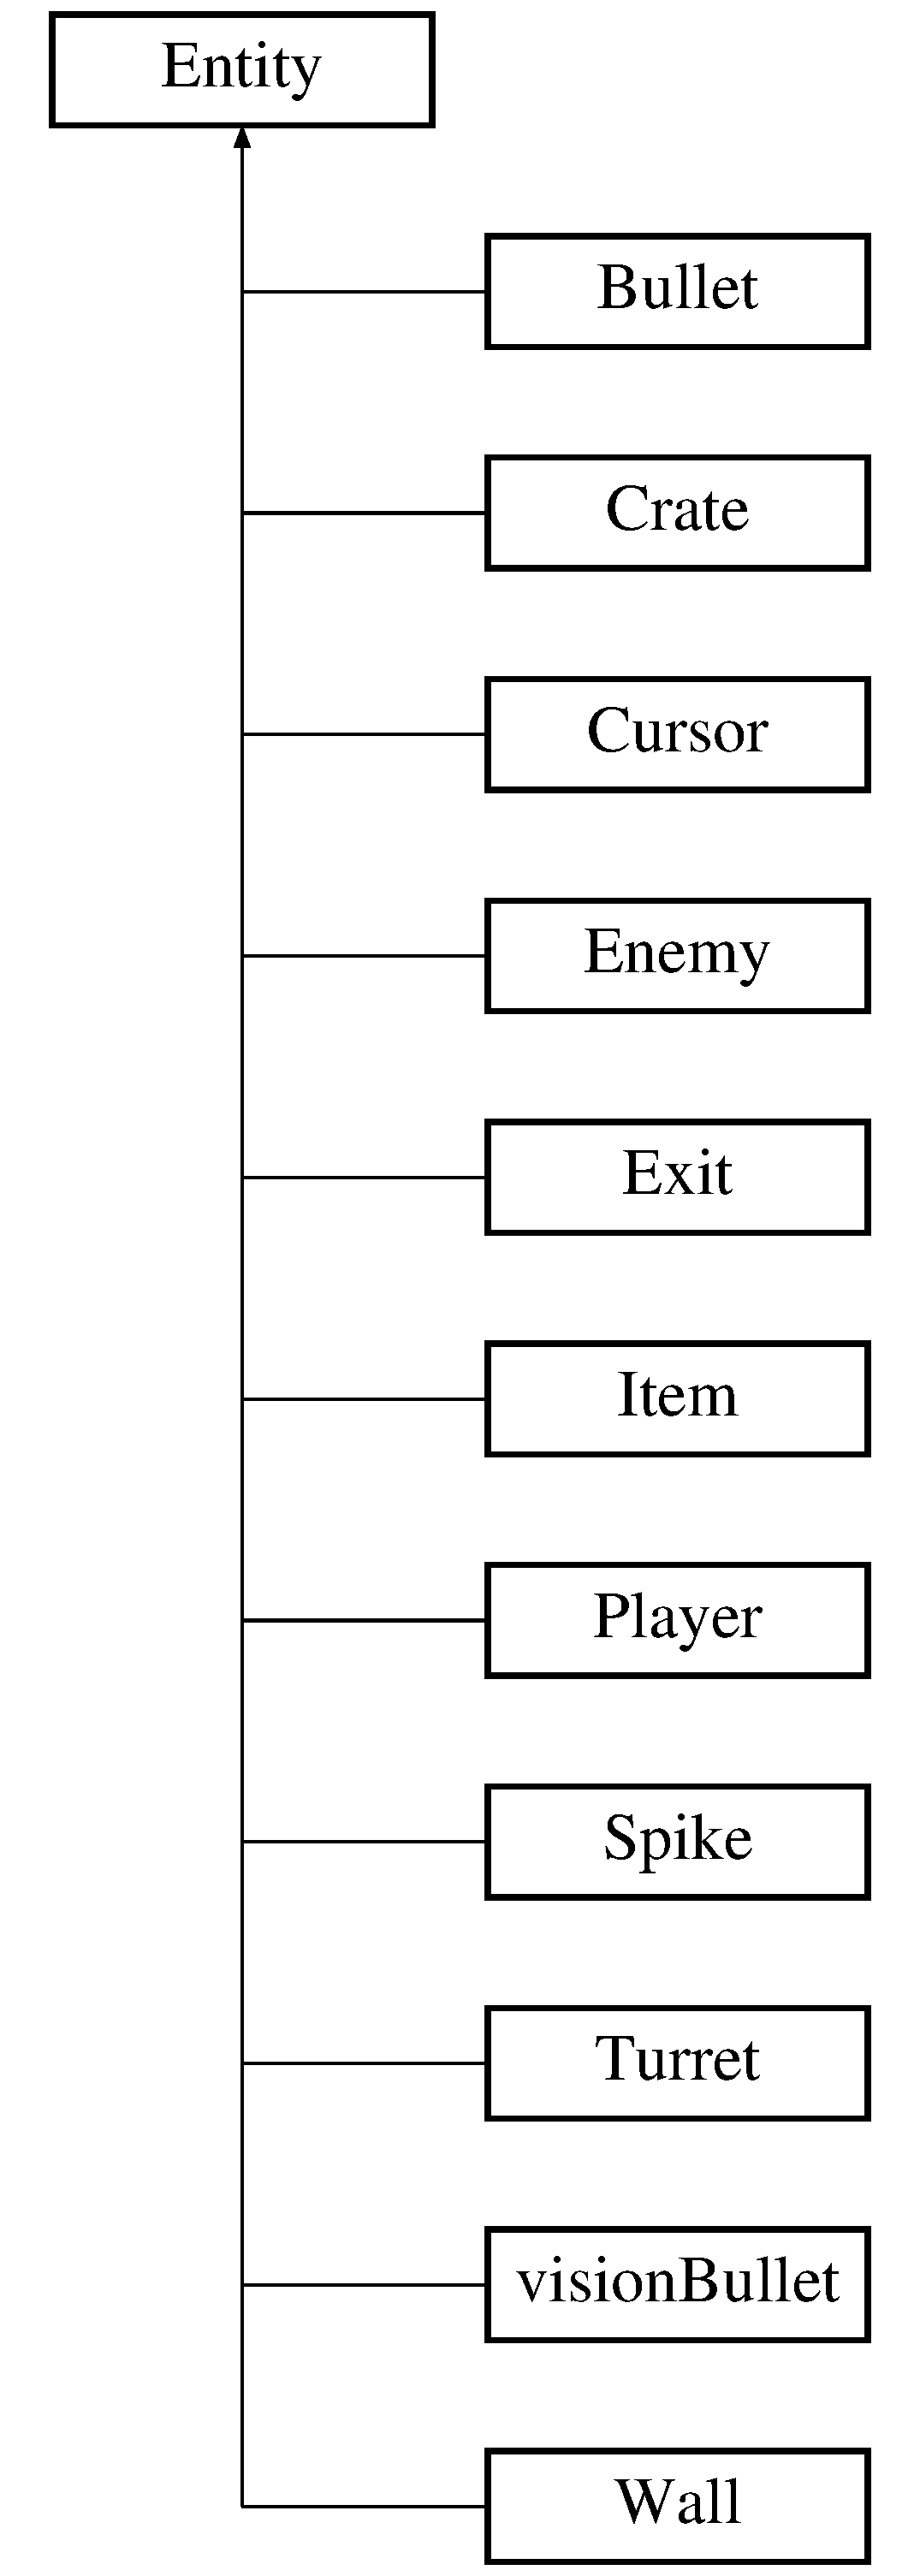
\includegraphics[height=12.000000cm]{class_entity}
\end{center}
\end{figure}
\subsection*{Public Member Functions}
\begin{DoxyCompactItemize}
\item 
\hyperlink{class_entity_a80b784625d59ece058c02726450127de}{Entity} (Vector2f \hyperlink{class_entity_a6af9d6498134ad0906011778bc5736db}{position}, Vector2f \hyperlink{class_entity_ae9a0a364c85f91ade5088b3610131417}{size}, bool \hyperlink{class_entity_af1b0754c9d5f4afa73834b23c6437101}{is\+Solid}, int \hyperlink{class_entity_a4edd9cc2506add0d9e27fade0bf957e8}{state}=0, bool \hyperlink{class_entity_a22234c0796f8c2ca0d116495c83ecdd6}{hostile}=false)
\item 
void \hyperlink{class_entity_a1d077cd5a6aa78265e4d9888cfc39d2c}{move} (Vector2f delta)
\begin{DoxyCompactList}\small\item\em move our entity by adding the parameter vector to our position. \end{DoxyCompactList}\item 
virtual bool \hyperlink{class_entity_af8678a1582e2a478d66df1ff29b66a0d}{collides\+With} (\hyperlink{class_entity}{Entity} $\ast$other, Vector2f delta=Vector2f(0, 0))
\begin{DoxyCompactList}\small\item\em Return whether or not this entity will collide with another when moved to a new position. \end{DoxyCompactList}\item 
virtual \hyperlink{class_entity}{Entity} $\ast$ \hyperlink{class_entity_a29117f3f40e7069d5d4c1b2fca7819d6}{hit} ()
\item 
virtual Vector2f \hyperlink{class_entity_a8b6080f0ab76702fcd00108aef8ea9dd}{get\+Pos} ()
\item 
virtual void \hyperlink{class_entity_aed73e98b980b85833428c935cc1c69f8}{update} ()
\item 
virtual void \hyperlink{class_entity_a030c3aa6641df7981a2d8a3fba890ec7}{draw} (Render\+Window \&w)
\end{DoxyCompactItemize}
\subsection*{Public Attributes}
\begin{DoxyCompactItemize}
\item 
Vector2f \hyperlink{class_entity_a6af9d6498134ad0906011778bc5736db}{position}
\item 
bool \hyperlink{class_entity_af1b0754c9d5f4afa73834b23c6437101}{is\+Solid}
\item 
int \hyperlink{class_entity_a4edd9cc2506add0d9e27fade0bf957e8}{state} = 0
\item 
bool \hyperlink{class_entity_a22234c0796f8c2ca0d116495c83ecdd6}{hostile} = false
\end{DoxyCompactItemize}
\subsection*{Protected Attributes}
\begin{DoxyCompactItemize}
\item 
Vector2f \hyperlink{class_entity_ae9a0a364c85f91ade5088b3610131417}{size}
\end{DoxyCompactItemize}


\subsection{Detailed Description}


Definition at line 19 of file Entity.\+h.



\subsection{Constructor \& Destructor Documentation}
\mbox{\Hypertarget{class_entity_a80b784625d59ece058c02726450127de}\label{class_entity_a80b784625d59ece058c02726450127de}} 
\index{Entity@{Entity}!Entity@{Entity}}
\index{Entity@{Entity}!Entity@{Entity}}
\subsubsection{\texorpdfstring{Entity()}{Entity()}}
{\footnotesize\ttfamily Entity\+::\+Entity (\begin{DoxyParamCaption}\item[{Vector2f}]{position,  }\item[{Vector2f}]{size,  }\item[{bool}]{is\+Solid,  }\item[{int}]{state = {\ttfamily 0},  }\item[{bool}]{hostile = {\ttfamily false} }\end{DoxyParamCaption})}



Definition at line 4 of file Entity.\+cpp.



\subsection{Member Function Documentation}
\mbox{\Hypertarget{class_entity_af8678a1582e2a478d66df1ff29b66a0d}\label{class_entity_af8678a1582e2a478d66df1ff29b66a0d}} 
\index{Entity@{Entity}!collides\+With@{collides\+With}}
\index{collides\+With@{collides\+With}!Entity@{Entity}}
\subsubsection{\texorpdfstring{collides\+With()}{collidesWith()}}
{\footnotesize\ttfamily bool Entity\+::collides\+With (\begin{DoxyParamCaption}\item[{\hyperlink{class_entity}{Entity} $\ast$}]{other,  }\item[{Vector2f}]{delta = {\ttfamily Vector2f(0,~0)} }\end{DoxyParamCaption})\hspace{0.3cm}{\ttfamily [virtual]}}



Return whether or not this entity will collide with another when moved to a new position. 



Definition at line 16 of file Entity.\+cpp.

\mbox{\Hypertarget{class_entity_a030c3aa6641df7981a2d8a3fba890ec7}\label{class_entity_a030c3aa6641df7981a2d8a3fba890ec7}} 
\index{Entity@{Entity}!draw@{draw}}
\index{draw@{draw}!Entity@{Entity}}
\subsubsection{\texorpdfstring{draw()}{draw()}}
{\footnotesize\ttfamily virtual void Entity\+::draw (\begin{DoxyParamCaption}\item[{Render\+Window \&}]{w }\end{DoxyParamCaption})\hspace{0.3cm}{\ttfamily [inline]}, {\ttfamily [virtual]}}



Reimplemented in \hyperlink{class_enemy_a582d09158d692070f4becf68220bf6b6}{Enemy}, \hyperlink{class_bullet_a14a795a7a6f4d0ad2e96a19b79afc5ee}{Bullet}, \hyperlink{class_player_a27ca9082a531285731af05f9395ffee8}{Player}, \hyperlink{classvision_bullet_ab2f4d4a63991b39480e3064ed5ee3809}{vision\+Bullet}, \hyperlink{class_cursor_a31c09a077d14237953223980197fdd17}{Cursor}, \hyperlink{class_crate_a2e9e544f1286c7de8830a8c2e7a955e9}{Crate}, \hyperlink{class_spike_a6f1baae74e1b5140459d2a439ad01547}{Spike}, and \hyperlink{class_turret_a7beef22798d993d9991bd22417034f49}{Turret}.



Definition at line 37 of file Entity.\+h.

\mbox{\Hypertarget{class_entity_a8b6080f0ab76702fcd00108aef8ea9dd}\label{class_entity_a8b6080f0ab76702fcd00108aef8ea9dd}} 
\index{Entity@{Entity}!get\+Pos@{get\+Pos}}
\index{get\+Pos@{get\+Pos}!Entity@{Entity}}
\subsubsection{\texorpdfstring{get\+Pos()}{getPos()}}
{\footnotesize\ttfamily virtual Vector2f Entity\+::get\+Pos (\begin{DoxyParamCaption}{ }\end{DoxyParamCaption})\hspace{0.3cm}{\ttfamily [inline]}, {\ttfamily [virtual]}}



Reimplemented in \hyperlink{class_enemy_a65af045027f5fd7396b420f0d4c34dac}{Enemy}, \hyperlink{class_player_a59cfaac9d09b12a290d2e89ca656be49}{Player}, \hyperlink{class_cursor_a214e135fad5e686f5bcfea34806c8730}{Cursor}, and \hyperlink{class_turret_a706e5a6001c3a0213b7510d4b99c0768}{Turret}.



Definition at line 35 of file Entity.\+h.

\mbox{\Hypertarget{class_entity_a29117f3f40e7069d5d4c1b2fca7819d6}\label{class_entity_a29117f3f40e7069d5d4c1b2fca7819d6}} 
\index{Entity@{Entity}!hit@{hit}}
\index{hit@{hit}!Entity@{Entity}}
\subsubsection{\texorpdfstring{hit()}{hit()}}
{\footnotesize\ttfamily virtual \hyperlink{class_entity}{Entity}$\ast$ Entity\+::hit (\begin{DoxyParamCaption}{ }\end{DoxyParamCaption})\hspace{0.3cm}{\ttfamily [inline]}, {\ttfamily [virtual]}}



Reimplemented in \hyperlink{class_enemy_a6cb8f8dbec88de9b2e95643709e349a3}{Enemy}, \hyperlink{class_player_a089d9293cc3be7e5d6d7c89b49538134}{Player}, \hyperlink{class_crate_a6e4a24b12c92e8576c107b60f0b8f1a8}{Crate}, and \hyperlink{class_turret_a141f76a3821b1d08a5aec057506c86e7}{Turret}.



Definition at line 34 of file Entity.\+h.

\mbox{\Hypertarget{class_entity_a1d077cd5a6aa78265e4d9888cfc39d2c}\label{class_entity_a1d077cd5a6aa78265e4d9888cfc39d2c}} 
\index{Entity@{Entity}!move@{move}}
\index{move@{move}!Entity@{Entity}}
\subsubsection{\texorpdfstring{move()}{move()}}
{\footnotesize\ttfamily void Entity\+::move (\begin{DoxyParamCaption}\item[{Vector2f}]{delta }\end{DoxyParamCaption})}



move our entity by adding the parameter vector to our position. 



Definition at line 12 of file Entity.\+cpp.

\mbox{\Hypertarget{class_entity_aed73e98b980b85833428c935cc1c69f8}\label{class_entity_aed73e98b980b85833428c935cc1c69f8}} 
\index{Entity@{Entity}!update@{update}}
\index{update@{update}!Entity@{Entity}}
\subsubsection{\texorpdfstring{update()}{update()}}
{\footnotesize\ttfamily virtual void Entity\+::update (\begin{DoxyParamCaption}{ }\end{DoxyParamCaption})\hspace{0.3cm}{\ttfamily [inline]}, {\ttfamily [virtual]}}



Reimplemented in \hyperlink{class_enemy_aa70d742da02995011f1618acc9e303db}{Enemy}, \hyperlink{class_bullet_a32f4a0611fe2dd245fee955d14ca1f68}{Bullet}, \hyperlink{class_player_a6912bb6e48efb5845d59f0f4582827ef}{Player}, \hyperlink{classvision_bullet_a425ac17ace4a29879a9a204ffc29021d}{vision\+Bullet}, \hyperlink{class_cursor_a2450501ae27244acb089209436d5b112}{Cursor}, \hyperlink{class_spike_a5f1fc626e9f58f4a08a002c6d2549942}{Spike}, and \hyperlink{class_turret_aad95afd1118f42d424465c14ebb445c7}{Turret}.



Definition at line 36 of file Entity.\+h.



\subsection{Member Data Documentation}
\mbox{\Hypertarget{class_entity_a22234c0796f8c2ca0d116495c83ecdd6}\label{class_entity_a22234c0796f8c2ca0d116495c83ecdd6}} 
\index{Entity@{Entity}!hostile@{hostile}}
\index{hostile@{hostile}!Entity@{Entity}}
\subsubsection{\texorpdfstring{hostile}{hostile}}
{\footnotesize\ttfamily bool Entity\+::hostile = false}



Definition at line 27 of file Entity.\+h.

\mbox{\Hypertarget{class_entity_af1b0754c9d5f4afa73834b23c6437101}\label{class_entity_af1b0754c9d5f4afa73834b23c6437101}} 
\index{Entity@{Entity}!is\+Solid@{is\+Solid}}
\index{is\+Solid@{is\+Solid}!Entity@{Entity}}
\subsubsection{\texorpdfstring{is\+Solid}{isSolid}}
{\footnotesize\ttfamily bool Entity\+::is\+Solid}



Definition at line 25 of file Entity.\+h.

\mbox{\Hypertarget{class_entity_a6af9d6498134ad0906011778bc5736db}\label{class_entity_a6af9d6498134ad0906011778bc5736db}} 
\index{Entity@{Entity}!position@{position}}
\index{position@{position}!Entity@{Entity}}
\subsubsection{\texorpdfstring{position}{position}}
{\footnotesize\ttfamily Vector2f Entity\+::position}



Definition at line 24 of file Entity.\+h.

\mbox{\Hypertarget{class_entity_ae9a0a364c85f91ade5088b3610131417}\label{class_entity_ae9a0a364c85f91ade5088b3610131417}} 
\index{Entity@{Entity}!size@{size}}
\index{size@{size}!Entity@{Entity}}
\subsubsection{\texorpdfstring{size}{size}}
{\footnotesize\ttfamily Vector2f Entity\+::size\hspace{0.3cm}{\ttfamily [protected]}}



Definition at line 22 of file Entity.\+h.

\mbox{\Hypertarget{class_entity_a4edd9cc2506add0d9e27fade0bf957e8}\label{class_entity_a4edd9cc2506add0d9e27fade0bf957e8}} 
\index{Entity@{Entity}!state@{state}}
\index{state@{state}!Entity@{Entity}}
\subsubsection{\texorpdfstring{state}{state}}
{\footnotesize\ttfamily int Entity\+::state = 0}



Definition at line 26 of file Entity.\+h.



The documentation for this class was generated from the following files\+:\begin{DoxyCompactItemize}
\item 
C\+:/\+Users/joost/\+Documents/\+Git\+Hub/topdown/\+Code/\+Team\+Topdown/\+Team\+Topdown/\hyperlink{_entity_8h}{Entity.\+h}\item 
C\+:/\+Users/joost/\+Documents/\+Git\+Hub/topdown/\+Code/\+Team\+Topdown/\+Team\+Topdown/\hyperlink{_entity_8cpp}{Entity.\+cpp}\end{DoxyCompactItemize}

\hypertarget{classentity_controller}{}\section{entity\+Controller Class Reference}
\label{classentity_controller}\index{entity\+Controller@{entity\+Controller}}


\hyperlink{class_entity}{Entity} class This class represents any entity in the game. It contains information about its position, size and whether it\textquotesingle{}s solid or not. It also has a function to change the position, a pure virtual update function and a function to determine collision via axis-\/aligned bounding boxes.  




{\ttfamily \#include $<$Entity.\+h$>$}



\subsection{Detailed Description}
\hyperlink{class_entity}{Entity} class This class represents any entity in the game. It contains information about its position, size and whether it\textquotesingle{}s solid or not. It also has a function to change the position, a pure virtual update function and a function to determine collision via axis-\/aligned bounding boxes. 

The documentation for this class was generated from the following file\+:\begin{DoxyCompactItemize}
\item 
C\+:/\+Users/joost/\+Documents/\+Git\+Hub/topdown/\+Code/\+Team\+Topdown/\+Team\+Topdown/\hyperlink{_entity_8h}{Entity.\+h}\end{DoxyCompactItemize}

\hypertarget{class_entity_controller}{}\section{Entity\+Controller Class Reference}
\label{class_entity_controller}\index{Entity\+Controller@{Entity\+Controller}}


Contains instances of every entity, including player and background. This class contains instances of every entity. It has a function to update positions of every entity, including player, taking collision into account. It also has a \hyperlink{class_entity_controller_a82e17378b1553449be6f93a8c18eefee}{draw()} function to draw all entities at once. Furthermore, it contains 4 vectors to determine direction, to be built into a seperate class.  




{\ttfamily \#include $<$Entity\+Controller.\+h$>$}

\subsection*{Public Member Functions}
\begin{DoxyCompactItemize}
\item 
\hyperlink{class_entity_controller_a2d81c913c30dc661d101c945d67b73b7}{Entity\+Controller} (\hyperlink{class_player}{Player} \&p, \hyperlink{class_cursor}{Cursor} \&c, \hyperlink{struct_controls_input}{Controls\+Input} \&ci, \hyperlink{class_map}{Map} $\ast$map)
\item 
\hyperlink{class_entity_controller_ad55bccfe26fd9a5486a749b2b49a0478}{$\sim$\+Entity\+Controller} ()
\item 
void \hyperlink{class_entity_controller_a8f0223a1a43a2369bc81dd53aadf251c}{melee\+Attack} ()
\item 
float \hyperlink{class_entity_controller_ab847c4e0ddefc7f23b2993c4cdc825a4}{calc\+Speed} ()
\item 
void \hyperlink{class_entity_controller_a1b1859bc8e5bfa72a0f1f34be3b1d5bd}{player\+Fire} ()
\item 
void \hyperlink{class_entity_controller_a3d7a4f7f330f070be70103bd00cf0f16}{update} ()
\item 
void \hyperlink{class_entity_controller_a82e17378b1553449be6f93a8c18eefee}{draw} (Render\+Window \&w)
\item 
int \hyperlink{class_entity_controller_a1df351e4f9a2870a265d07fe8d082efd}{exiting} ()
\end{DoxyCompactItemize}
\subsection*{Public Attributes}
\begin{DoxyCompactItemize}
\item 
\hyperlink{struct_timer}{Timer} \hyperlink{class_entity_controller_a05eb6c6b51a8628079e3c9432319f2b5}{shake\+Timer}
\end{DoxyCompactItemize}


\subsection{Detailed Description}
Contains instances of every entity, including player and background. This class contains instances of every entity. It has a function to update positions of every entity, including player, taking collision into account. It also has a \hyperlink{class_entity_controller_a82e17378b1553449be6f93a8c18eefee}{draw()} function to draw all entities at once. Furthermore, it contains 4 vectors to determine direction, to be built into a seperate class. 

Definition at line 23 of file Entity\+Controller.\+h.



\subsection{Constructor \& Destructor Documentation}
\mbox{\Hypertarget{class_entity_controller_a2d81c913c30dc661d101c945d67b73b7}\label{class_entity_controller_a2d81c913c30dc661d101c945d67b73b7}} 
\index{Entity\+Controller@{Entity\+Controller}!Entity\+Controller@{Entity\+Controller}}
\index{Entity\+Controller@{Entity\+Controller}!Entity\+Controller@{Entity\+Controller}}
\subsubsection{\texorpdfstring{Entity\+Controller()}{EntityController()}}
{\footnotesize\ttfamily Entity\+Controller\+::\+Entity\+Controller (\begin{DoxyParamCaption}\item[{\hyperlink{class_player}{Player} \&}]{p,  }\item[{\hyperlink{class_cursor}{Cursor} \&}]{c,  }\item[{\hyperlink{struct_controls_input}{Controls\+Input} \&}]{ci,  }\item[{\hyperlink{class_map}{Map} $\ast$}]{map }\end{DoxyParamCaption})}



Definition at line 4 of file Entity\+Controller.\+cpp.

\mbox{\Hypertarget{class_entity_controller_ad55bccfe26fd9a5486a749b2b49a0478}\label{class_entity_controller_ad55bccfe26fd9a5486a749b2b49a0478}} 
\index{Entity\+Controller@{Entity\+Controller}!````~Entity\+Controller@{$\sim$\+Entity\+Controller}}
\index{````~Entity\+Controller@{$\sim$\+Entity\+Controller}!Entity\+Controller@{Entity\+Controller}}
\subsubsection{\texorpdfstring{$\sim$\+Entity\+Controller()}{~EntityController()}}
{\footnotesize\ttfamily Entity\+Controller\+::$\sim$\+Entity\+Controller (\begin{DoxyParamCaption}{ }\end{DoxyParamCaption})}



Definition at line 28 of file Entity\+Controller.\+cpp.



\subsection{Member Function Documentation}
\mbox{\Hypertarget{class_entity_controller_ab847c4e0ddefc7f23b2993c4cdc825a4}\label{class_entity_controller_ab847c4e0ddefc7f23b2993c4cdc825a4}} 
\index{Entity\+Controller@{Entity\+Controller}!calc\+Speed@{calc\+Speed}}
\index{calc\+Speed@{calc\+Speed}!Entity\+Controller@{Entity\+Controller}}
\subsubsection{\texorpdfstring{calc\+Speed()}{calcSpeed()}}
{\footnotesize\ttfamily float Entity\+Controller\+::calc\+Speed (\begin{DoxyParamCaption}{ }\end{DoxyParamCaption})}

/float \hyperlink{class_entity_controller_ab847c4e0ddefc7f23b2993c4cdc825a4}{calc\+Speed()} /brief checks what speed to return based on keyboard inputs 

Definition at line 112 of file Entity\+Controller.\+cpp.

\mbox{\Hypertarget{class_entity_controller_a82e17378b1553449be6f93a8c18eefee}\label{class_entity_controller_a82e17378b1553449be6f93a8c18eefee}} 
\index{Entity\+Controller@{Entity\+Controller}!draw@{draw}}
\index{draw@{draw}!Entity\+Controller@{Entity\+Controller}}
\subsubsection{\texorpdfstring{draw()}{draw()}}
{\footnotesize\ttfamily void Entity\+Controller\+::draw (\begin{DoxyParamCaption}\item[{Render\+Window \&}]{w }\end{DoxyParamCaption})}

/void \hyperlink{class_entity_controller_a82e17378b1553449be6f93a8c18eefee}{draw()} /brief draws the following objects on the screen\+:
\begin{DoxyItemize}
\item entities
\item bullets
\item items
\item player
\item hud
\item cursor
\item background 
\end{DoxyItemize}

Definition at line 394 of file Entity\+Controller.\+cpp.

\mbox{\Hypertarget{class_entity_controller_a1df351e4f9a2870a265d07fe8d082efd}\label{class_entity_controller_a1df351e4f9a2870a265d07fe8d082efd}} 
\index{Entity\+Controller@{Entity\+Controller}!exiting@{exiting}}
\index{exiting@{exiting}!Entity\+Controller@{Entity\+Controller}}
\subsubsection{\texorpdfstring{exiting()}{exiting()}}
{\footnotesize\ttfamily int Entity\+Controller\+::exiting (\begin{DoxyParamCaption}{ }\end{DoxyParamCaption})}



Definition at line 419 of file Entity\+Controller.\+cpp.

\mbox{\Hypertarget{class_entity_controller_a8f0223a1a43a2369bc81dd53aadf251c}\label{class_entity_controller_a8f0223a1a43a2369bc81dd53aadf251c}} 
\index{Entity\+Controller@{Entity\+Controller}!melee\+Attack@{melee\+Attack}}
\index{melee\+Attack@{melee\+Attack}!Entity\+Controller@{Entity\+Controller}}
\subsubsection{\texorpdfstring{melee\+Attack()}{meleeAttack()}}
{\footnotesize\ttfamily void Entity\+Controller\+::melee\+Attack (\begin{DoxyParamCaption}{ }\end{DoxyParamCaption})}



Definition at line 51 of file Entity\+Controller.\+cpp.

\mbox{\Hypertarget{class_entity_controller_a1b1859bc8e5bfa72a0f1f34be3b1d5bd}\label{class_entity_controller_a1b1859bc8e5bfa72a0f1f34be3b1d5bd}} 
\index{Entity\+Controller@{Entity\+Controller}!player\+Fire@{player\+Fire}}
\index{player\+Fire@{player\+Fire}!Entity\+Controller@{Entity\+Controller}}
\subsubsection{\texorpdfstring{player\+Fire()}{playerFire()}}
{\footnotesize\ttfamily void Entity\+Controller\+::player\+Fire (\begin{DoxyParamCaption}{ }\end{DoxyParamCaption})}

/void \hyperlink{class_entity_controller_a1b1859bc8e5bfa72a0f1f34be3b1d5bd}{player\+Fire()} /brief checks whether the player is shooting or not and fires bullets based on the keyboard inputs 

Definition at line 141 of file Entity\+Controller.\+cpp.

\mbox{\Hypertarget{class_entity_controller_a3d7a4f7f330f070be70103bd00cf0f16}\label{class_entity_controller_a3d7a4f7f330f070be70103bd00cf0f16}} 
\index{Entity\+Controller@{Entity\+Controller}!update@{update}}
\index{update@{update}!Entity\+Controller@{Entity\+Controller}}
\subsubsection{\texorpdfstring{update()}{update()}}
{\footnotesize\ttfamily void Entity\+Controller\+::update (\begin{DoxyParamCaption}{ }\end{DoxyParamCaption})}

/void \hyperlink{class_entity_controller_a3d7a4f7f330f070be70103bd00cf0f16}{update()} /brief updates the following within this object\+:
\begin{DoxyItemize}
\item sets the shake\+Timer to shake the screen
\item checks if the player is dead
\item checks whether the player is moving or not
\item moves the player
\item checks entity colissions
\item checks bullets on map 
\end{DoxyItemize}

Definition at line 202 of file Entity\+Controller.\+cpp.



\subsection{Member Data Documentation}
\mbox{\Hypertarget{class_entity_controller_a05eb6c6b51a8628079e3c9432319f2b5}\label{class_entity_controller_a05eb6c6b51a8628079e3c9432319f2b5}} 
\index{Entity\+Controller@{Entity\+Controller}!shake\+Timer@{shake\+Timer}}
\index{shake\+Timer@{shake\+Timer}!Entity\+Controller@{Entity\+Controller}}
\subsubsection{\texorpdfstring{shake\+Timer}{shakeTimer}}
{\footnotesize\ttfamily \hyperlink{struct_timer}{Timer} Entity\+Controller\+::shake\+Timer}

creates a timer that contains data for shake 

Definition at line 61 of file Entity\+Controller.\+h.



The documentation for this class was generated from the following files\+:\begin{DoxyCompactItemize}
\item 
C\+:/\+Users/joost/\+Documents/\+Git\+Hub/topdown/\+Code/\+Team\+Topdown/\+Team\+Topdown/\hyperlink{_entity_controller_8h}{Entity\+Controller.\+h}\item 
C\+:/\+Users/joost/\+Documents/\+Git\+Hub/topdown/\+Code/\+Team\+Topdown/\+Team\+Topdown/\hyperlink{_entity_controller_8cpp}{Entity\+Controller.\+cpp}\end{DoxyCompactItemize}

\hypertarget{class_exit}{}\section{Exit Class Reference}
\label{class_exit}\index{Exit@{Exit}}


Invisible wall which handles \textquotesingle{}exiting\textquotesingle{} a level. The wall contains a number representing the level to advance to. It uses standard A\+A\+B\+B-\/collision detection to determine if our player collides. The exit number is saved in the state and read by EC to determine where to exit to.  




{\ttfamily \#include $<$Exit.\+h$>$}

Inheritance diagram for Exit\+:\begin{figure}[H]
\begin{center}
\leavevmode
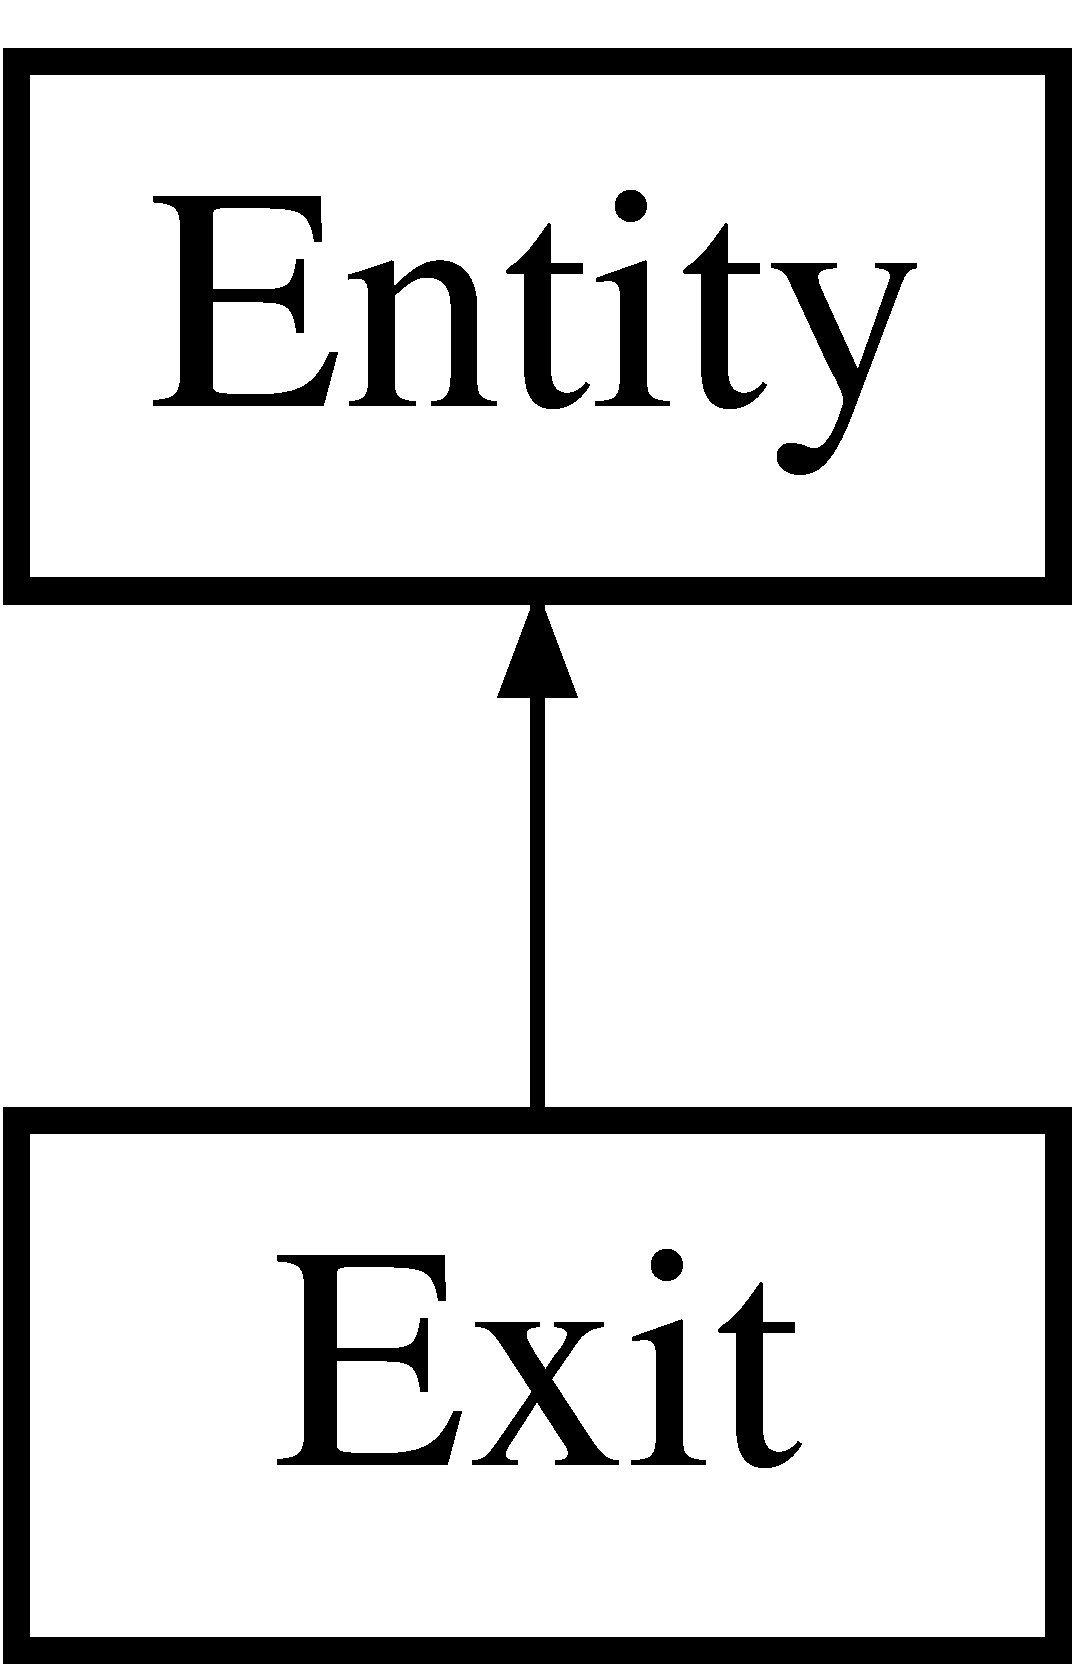
\includegraphics[height=2.000000cm]{class_exit}
\end{center}
\end{figure}
\subsection*{Public Member Functions}
\begin{DoxyCompactItemize}
\item 
\hyperlink{class_exit_ab98655fa93983e9b83175f68c35513de}{Exit} (Vector2f \hyperlink{class_entity_a6af9d6498134ad0906011778bc5736db}{position}, int exit\+Nr, Vector2f \hyperlink{class_entity_ae9a0a364c85f91ade5088b3610131417}{size}=Vector2f(32.\+0f, 32.\+0f), bool is\+Solid=false)
\end{DoxyCompactItemize}
\subsection*{Additional Inherited Members}


\subsection{Detailed Description}
Invisible wall which handles \textquotesingle{}exiting\textquotesingle{} a level. The wall contains a number representing the level to advance to. It uses standard A\+A\+B\+B-\/collision detection to determine if our player collides. The exit number is saved in the state and read by EC to determine where to exit to. 

Definition at line 10 of file Exit.\+h.



\subsection{Constructor \& Destructor Documentation}
\mbox{\Hypertarget{class_exit_ab98655fa93983e9b83175f68c35513de}\label{class_exit_ab98655fa93983e9b83175f68c35513de}} 
\index{Exit@{Exit}!Exit@{Exit}}
\index{Exit@{Exit}!Exit@{Exit}}
\subsubsection{\texorpdfstring{Exit()}{Exit()}}
{\footnotesize\ttfamily Exit\+::\+Exit (\begin{DoxyParamCaption}\item[{Vector2f}]{position,  }\item[{int}]{exit\+Nr,  }\item[{Vector2f}]{size = {\ttfamily Vector2f(32.0f,~32.0f)},  }\item[{bool}]{is\+Solid = {\ttfamily false} }\end{DoxyParamCaption})}



Definition at line 4 of file Exit.\+cpp.



The documentation for this class was generated from the following files\+:\begin{DoxyCompactItemize}
\item 
C\+:/\+Users/joost/\+Documents/\+Git\+Hub/topdown/\+Code/\+Team\+Topdown/\+Team\+Topdown/\hyperlink{_exit_8h}{Exit.\+h}\item 
C\+:/\+Users/joost/\+Documents/\+Git\+Hub/topdown/\+Code/\+Team\+Topdown/\+Team\+Topdown/\hyperlink{_exit_8cpp}{Exit.\+cpp}\end{DoxyCompactItemize}

\hypertarget{class_game_loop_object}{}\section{Game\+Loop\+Object Class Reference}
\label{class_game_loop_object}\index{Game\+Loop\+Object@{Game\+Loop\+Object}}


The base class for all objects used in a game loop.  




{\ttfamily \#include $<$Game\+Loop\+Object.\+hpp$>$}

Inheritance diagram for Game\+Loop\+Object\+:\begin{figure}[H]
\begin{center}
\leavevmode
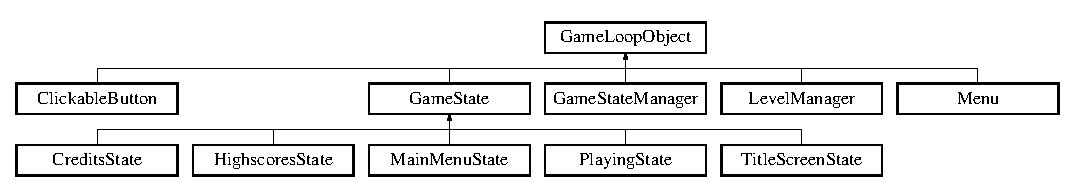
\includegraphics[height=2.137405cm]{class_game_loop_object}
\end{center}
\end{figure}
\subsection*{Public Member Functions}
\begin{DoxyCompactItemize}
\item 
\hyperlink{class_game_loop_object_aa5e0d6adf075fe106b7da8c1c6b19d6b}{Game\+Loop\+Object} ()
\begin{DoxyCompactList}\small\item\em Constructor method. \end{DoxyCompactList}\item 
virtual \hyperlink{class_game_loop_object_afec283bec43cc40dc49c54a7641b4915}{$\sim$\+Game\+Loop\+Object} ()
\begin{DoxyCompactList}\small\item\em Destructor method. \end{DoxyCompactList}\item 
virtual void \hyperlink{class_game_loop_object_ae36a15981f1dd3f3bea6050473490349}{Update} ()
\begin{DoxyCompactList}\small\item\em virtual update method to be used in a game loop. \end{DoxyCompactList}\item 
virtual void \hyperlink{class_game_loop_object_a0572a88e5b98fa8a41078260d152202d}{Draw} (sf\+::\+Render\+Window \&window)
\begin{DoxyCompactList}\small\item\em virtual draw method to be used in a game loop. \end{DoxyCompactList}\item 
virtual void \hyperlink{class_game_loop_object_aecab111d504b7f4590045ca7c83a36de}{Handle\+Input} ()
\begin{DoxyCompactList}\small\item\em virtual Handle\+Input method to be used in a game loop. \end{DoxyCompactList}\item 
virtual void \hyperlink{class_game_loop_object_af61e973be170cb9437a5b7d9ecd6ef53}{Reset} ()
\begin{DoxyCompactList}\small\item\em virtual reset method to reset the object to default startup parameters. \end{DoxyCompactList}\end{DoxyCompactItemize}


\subsection{Detailed Description}
The base class for all objects used in a game loop. 

This class is abstract, only having the virtual methods Handle\+Input, Update, Draw and Reset. Currently, both \hyperlink{class_game_state_manager}{Game\+State\+Manager} and \hyperlink{class_game_state}{Game\+State} inherit this class, while \hyperlink{class_game_state}{Game\+State} doesn\textquotesingle{}t add anything new, so it is basically the same class under a different name. We should decide if we merge \hyperlink{class_game_loop_object}{Game\+Loop\+Object} and \hyperlink{class_game_state}{Game\+State} or if we add more functionality to \hyperlink{class_game_state}{Game\+State}. 

Definition at line 14 of file Game\+Loop\+Object.\+hpp.



\subsection{Constructor \& Destructor Documentation}
\mbox{\Hypertarget{class_game_loop_object_aa5e0d6adf075fe106b7da8c1c6b19d6b}\label{class_game_loop_object_aa5e0d6adf075fe106b7da8c1c6b19d6b}} 
\index{Game\+Loop\+Object@{Game\+Loop\+Object}!Game\+Loop\+Object@{Game\+Loop\+Object}}
\index{Game\+Loop\+Object@{Game\+Loop\+Object}!Game\+Loop\+Object@{Game\+Loop\+Object}}
\subsubsection{\texorpdfstring{Game\+Loop\+Object()}{GameLoopObject()}}
{\footnotesize\ttfamily Game\+Loop\+Object\+::\+Game\+Loop\+Object (\begin{DoxyParamCaption}{ }\end{DoxyParamCaption})}



Constructor method. 

Empty constructor method taking no arguments. 

Definition at line 4 of file Game\+Loop\+Object.\+cpp.

\mbox{\Hypertarget{class_game_loop_object_afec283bec43cc40dc49c54a7641b4915}\label{class_game_loop_object_afec283bec43cc40dc49c54a7641b4915}} 
\index{Game\+Loop\+Object@{Game\+Loop\+Object}!````~Game\+Loop\+Object@{$\sim$\+Game\+Loop\+Object}}
\index{````~Game\+Loop\+Object@{$\sim$\+Game\+Loop\+Object}!Game\+Loop\+Object@{Game\+Loop\+Object}}
\subsubsection{\texorpdfstring{$\sim$\+Game\+Loop\+Object()}{~GameLoopObject()}}
{\footnotesize\ttfamily Game\+Loop\+Object\+::$\sim$\+Game\+Loop\+Object (\begin{DoxyParamCaption}{ }\end{DoxyParamCaption})\hspace{0.3cm}{\ttfamily [virtual]}}



Destructor method. 

Empty destructor. 

Definition at line 14 of file Game\+Loop\+Object.\+cpp.



\subsection{Member Function Documentation}
\mbox{\Hypertarget{class_game_loop_object_a0572a88e5b98fa8a41078260d152202d}\label{class_game_loop_object_a0572a88e5b98fa8a41078260d152202d}} 
\index{Game\+Loop\+Object@{Game\+Loop\+Object}!Draw@{Draw}}
\index{Draw@{Draw}!Game\+Loop\+Object@{Game\+Loop\+Object}}
\subsubsection{\texorpdfstring{Draw()}{Draw()}}
{\footnotesize\ttfamily void Game\+Loop\+Object\+::\+Draw (\begin{DoxyParamCaption}\item[{sf\+::\+Render\+Window \&}]{window }\end{DoxyParamCaption})\hspace{0.3cm}{\ttfamily [virtual]}}



virtual draw method to be used in a game loop. 

a virtual method. child class should implement its own functionality. 

Reimplemented in \hyperlink{class_game_state_manager_a4d42ae9f3b8c87f420fc79fd716e0c17}{Game\+State\+Manager}, \hyperlink{class_playing_state_a6f5feffc1c6de994450828fbe2f5c173}{Playing\+State}, \hyperlink{class_main_menu_state_a6965e10d73953ef09c63a64685136307}{Main\+Menu\+State}, \hyperlink{class_menu_a9052b7f20dcf6d9ed47d87f16fcfe5e9}{Menu}, \hyperlink{class_clickable_button_a55b5a7b941f25066a8d0481326794b62}{Clickable\+Button}, \hyperlink{class_title_screen_state_a1e1022947dac4a9b69c6bde57fe52217}{Title\+Screen\+State}, \hyperlink{class_highscores_state_a50fc2005675f2cc1740e3f9ef698bdab}{Highscores\+State}, \hyperlink{class_level_manager_a35cafa518fbbb9fdedfc6a587772bed9}{Level\+Manager}, \hyperlink{class_credits_state_a085e7decf7f1fc7edae68db50851b84a}{Credits\+State}, and \hyperlink{class_game_state_a8741c5c696c6c366beb4b845c08c3cf8}{Game\+State}.



Definition at line 10 of file Game\+Loop\+Object.\+cpp.

\mbox{\Hypertarget{class_game_loop_object_aecab111d504b7f4590045ca7c83a36de}\label{class_game_loop_object_aecab111d504b7f4590045ca7c83a36de}} 
\index{Game\+Loop\+Object@{Game\+Loop\+Object}!Handle\+Input@{Handle\+Input}}
\index{Handle\+Input@{Handle\+Input}!Game\+Loop\+Object@{Game\+Loop\+Object}}
\subsubsection{\texorpdfstring{Handle\+Input()}{HandleInput()}}
{\footnotesize\ttfamily void Game\+Loop\+Object\+::\+Handle\+Input (\begin{DoxyParamCaption}{ }\end{DoxyParamCaption})\hspace{0.3cm}{\ttfamily [virtual]}}



virtual Handle\+Input method to be used in a game loop. 

a virtual method. child class should implement its own functionality. 

Reimplemented in \hyperlink{class_game_state_manager_a6546ed46ea23d9a9206c7d540e8b3b3b}{Game\+State\+Manager}, \hyperlink{class_playing_state_ab61fc6f59f00ccf5db80f67d5e4c50a1}{Playing\+State}, \hyperlink{class_main_menu_state_ac332ae234d282f4e6657ee9d0685b7ff}{Main\+Menu\+State}, \hyperlink{class_menu_a0cb3596524ed7fd021f999860b563bf8}{Menu}, \hyperlink{class_clickable_button_a939a1f2a5414c37e9c1c1310db576224}{Clickable\+Button}, \hyperlink{class_game_state_a8bce2828cee99ae7c07322804531fd01}{Game\+State}, \hyperlink{class_title_screen_state_a1bad900daba7f6481632a58212f39af0}{Title\+Screen\+State}, \hyperlink{class_highscores_state_aa8ce1b29acad9790ff065e5c96635c85}{Highscores\+State}, and \hyperlink{class_credits_state_a63557b2290a2febb88e78ae90754a7ec}{Credits\+State}.



Definition at line 6 of file Game\+Loop\+Object.\+cpp.

\mbox{\Hypertarget{class_game_loop_object_af61e973be170cb9437a5b7d9ecd6ef53}\label{class_game_loop_object_af61e973be170cb9437a5b7d9ecd6ef53}} 
\index{Game\+Loop\+Object@{Game\+Loop\+Object}!Reset@{Reset}}
\index{Reset@{Reset}!Game\+Loop\+Object@{Game\+Loop\+Object}}
\subsubsection{\texorpdfstring{Reset()}{Reset()}}
{\footnotesize\ttfamily void Game\+Loop\+Object\+::\+Reset (\begin{DoxyParamCaption}{ }\end{DoxyParamCaption})\hspace{0.3cm}{\ttfamily [virtual]}}



virtual reset method to reset the object to default startup parameters. 

a virtual method. child class should implement its own functionality. 

Reimplemented in \hyperlink{class_game_state_manager_ab92faa645a6049828d6a4048779e0aee}{Game\+State\+Manager}, \hyperlink{class_main_menu_state_a6f6c9814913db12bc9578411620f9b56}{Main\+Menu\+State}, \hyperlink{class_menu_af48862906748cee615d455eae4ee3349}{Menu}, \hyperlink{class_clickable_button_a01ae3f140debdc8b525e1ef745bdbff3}{Clickable\+Button}, \hyperlink{class_title_screen_state_a7e6cf3ef5534f42a4ca1e75045a45c71}{Title\+Screen\+State}, \hyperlink{class_game_state_a46ac6317883dff0eba4f8f305af6b6bb}{Game\+State}, \hyperlink{class_highscores_state_a6368de23eaf55fa1cd40cba04cbd07a0}{Highscores\+State}, \hyperlink{class_level_manager_a5e1dd3b7ca877857f1246c7fc95b6a3f}{Level\+Manager}, and \hyperlink{class_credits_state_ad87636e8b9438092bd0151185f385c17}{Credits\+State}.



Definition at line 12 of file Game\+Loop\+Object.\+cpp.

\mbox{\Hypertarget{class_game_loop_object_ae36a15981f1dd3f3bea6050473490349}\label{class_game_loop_object_ae36a15981f1dd3f3bea6050473490349}} 
\index{Game\+Loop\+Object@{Game\+Loop\+Object}!Update@{Update}}
\index{Update@{Update}!Game\+Loop\+Object@{Game\+Loop\+Object}}
\subsubsection{\texorpdfstring{Update()}{Update()}}
{\footnotesize\ttfamily void Game\+Loop\+Object\+::\+Update (\begin{DoxyParamCaption}{ }\end{DoxyParamCaption})\hspace{0.3cm}{\ttfamily [virtual]}}



virtual update method to be used in a game loop. 

a virtual method. child class should implement its own functionality. 

Reimplemented in \hyperlink{class_game_state_manager_a749124e1fcaaa5eae4578bf8e3f6e4d5}{Game\+State\+Manager}, \hyperlink{class_playing_state_afb7ccd732dfaad4397b5096876092136}{Playing\+State}, \hyperlink{class_main_menu_state_a35ec35095919057ef7373906b09a9d30}{Main\+Menu\+State}, \hyperlink{class_menu_af29d71473a414e31e914bc637840cb3e}{Menu}, \hyperlink{class_clickable_button_a393e1529583626f6ee52f0955bd68da8}{Clickable\+Button}, \hyperlink{class_title_screen_state_a0db8d35f9d3013155d2e61939d2a47ea}{Title\+Screen\+State}, \hyperlink{class_highscores_state_a8a55079503b5bdaf205e74eb9d48dae0}{Highscores\+State}, \hyperlink{class_level_manager_a7800611361e7c2ae99102e69429456fc}{Level\+Manager}, \hyperlink{class_credits_state_a565adc4ac454f23941c5db684da56ad7}{Credits\+State}, and \hyperlink{class_game_state_a5be51b634f95bc6e57066ad6931aa18b}{Game\+State}.



Definition at line 8 of file Game\+Loop\+Object.\+cpp.



The documentation for this class was generated from the following files\+:\begin{DoxyCompactItemize}
\item 
C\+:/\+Users/joost/\+Documents/\+Git\+Hub/topdown/\+Code/\+Team\+Topdown/\+Team\+Topdown/\hyperlink{_game_loop_object_8hpp}{Game\+Loop\+Object.\+hpp}\item 
C\+:/\+Users/joost/\+Documents/\+Git\+Hub/topdown/\+Code/\+Team\+Topdown/\+Team\+Topdown/\hyperlink{_game_loop_object_8cpp}{Game\+Loop\+Object.\+cpp}\end{DoxyCompactItemize}

\hypertarget{class_game_state}{}\section{Game\+State Class Reference}
\label{class_game_state}\index{Game\+State@{Game\+State}}


The base class for all gamestates.  




{\ttfamily \#include $<$Game\+State.\+hpp$>$}

Inheritance diagram for Game\+State\+:\begin{figure}[H]
\begin{center}
\leavevmode
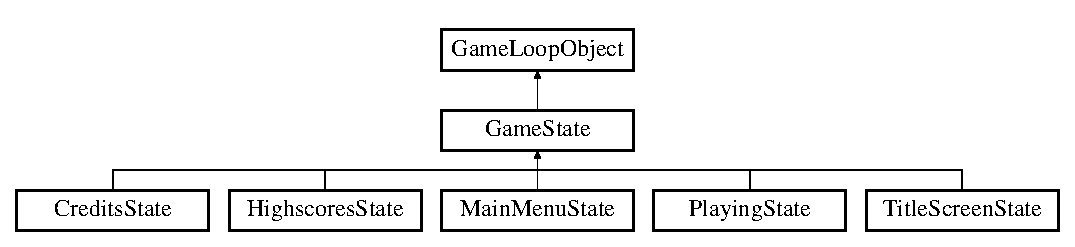
\includegraphics[height=2.871795cm]{class_game_state}
\end{center}
\end{figure}
\subsection*{Public Member Functions}
\begin{DoxyCompactItemize}
\item 
\hyperlink{class_game_state_a4fa0a2bf50315c4a35a3890a0adcee5c}{Game\+State} ()
\begin{DoxyCompactList}\small\item\em Constructor method. \end{DoxyCompactList}\item 
virtual \hyperlink{class_game_state_ae623df5042cd0c17daa3394fdcb397b3}{$\sim$\+Game\+State} ()
\begin{DoxyCompactList}\small\item\em Destructor method. \end{DoxyCompactList}\item 
virtual void \hyperlink{class_game_state_a5be51b634f95bc6e57066ad6931aa18b}{Update} ()
\begin{DoxyCompactList}\small\item\em Virtual update method to be used in a game loop. \end{DoxyCompactList}\item 
virtual void \hyperlink{class_game_state_a8741c5c696c6c366beb4b845c08c3cf8}{Draw} (sf\+::\+Render\+Window \&window)
\begin{DoxyCompactList}\small\item\em virtual draw method to be used in a game loop. \end{DoxyCompactList}\item 
virtual void \hyperlink{class_game_state_a8bce2828cee99ae7c07322804531fd01}{Handle\+Input} ()
\begin{DoxyCompactList}\small\item\em virtual Handle\+Input method to be used in a game loop. \end{DoxyCompactList}\item 
virtual void \hyperlink{class_game_state_a46ac6317883dff0eba4f8f305af6b6bb}{Reset} ()
\begin{DoxyCompactList}\small\item\em virtual reset method to reset the gamestate to default. \end{DoxyCompactList}\end{DoxyCompactItemize}


\subsection{Detailed Description}
The base class for all gamestates. 

This class is abstract. This class is a \hyperlink{class_game_loop_object}{Game\+Loop\+Object} and adds nothing new. It is basically the same class under a different name. Eventually it should be decided if more functionality is to be added to this class or if it is going to be merged with \hyperlink{class_game_loop_object}{Game\+Loop\+Object}. \hyperlink{class_game_state}{Game\+State} has the following virtual methods\+:
\begin{DoxyItemize}
\item \hyperlink{class_game_state_a5be51b634f95bc6e57066ad6931aa18b}{Update()}
\item \hyperlink{class_game_state_a8741c5c696c6c366beb4b845c08c3cf8}{Draw()}
\item \hyperlink{class_game_state_a8bce2828cee99ae7c07322804531fd01}{Handle\+Input()}
\item \hyperlink{class_game_state_a46ac6317883dff0eba4f8f305af6b6bb}{Reset()} An implementation of a gamestate must implement all of these methods so that the \hyperlink{class_game_state_manager}{Game\+State\+Manager} can call update, draw and handleinput 60 times per second in the game loop and reset the gamestate when necessary. The \hyperlink{class_game_state_manager}{Game\+State\+Manager} can only run one gamestate at a time and each gamestate must be designed with this in mind. When one gamestate is running, all other gamestates are paused as they are not updated. 
\end{DoxyItemize}

Definition at line 28 of file Game\+State.\+hpp.



\subsection{Constructor \& Destructor Documentation}
\mbox{\Hypertarget{class_game_state_a4fa0a2bf50315c4a35a3890a0adcee5c}\label{class_game_state_a4fa0a2bf50315c4a35a3890a0adcee5c}} 
\index{Game\+State@{Game\+State}!Game\+State@{Game\+State}}
\index{Game\+State@{Game\+State}!Game\+State@{Game\+State}}
\subsubsection{\texorpdfstring{Game\+State()}{GameState()}}
{\footnotesize\ttfamily Game\+State\+::\+Game\+State (\begin{DoxyParamCaption}{ }\end{DoxyParamCaption})}



Constructor method. 

Empty constructor method taking no arguments. 

Definition at line 4 of file Game\+State.\+cpp.

\mbox{\Hypertarget{class_game_state_ae623df5042cd0c17daa3394fdcb397b3}\label{class_game_state_ae623df5042cd0c17daa3394fdcb397b3}} 
\index{Game\+State@{Game\+State}!````~Game\+State@{$\sim$\+Game\+State}}
\index{````~Game\+State@{$\sim$\+Game\+State}!Game\+State@{Game\+State}}
\subsubsection{\texorpdfstring{$\sim$\+Game\+State()}{~GameState()}}
{\footnotesize\ttfamily Game\+State\+::$\sim$\+Game\+State (\begin{DoxyParamCaption}{ }\end{DoxyParamCaption})\hspace{0.3cm}{\ttfamily [virtual]}}



Destructor method. 

Empty destructor method taking no arguments. 

Definition at line 14 of file Game\+State.\+cpp.



\subsection{Member Function Documentation}
\mbox{\Hypertarget{class_game_state_a8741c5c696c6c366beb4b845c08c3cf8}\label{class_game_state_a8741c5c696c6c366beb4b845c08c3cf8}} 
\index{Game\+State@{Game\+State}!Draw@{Draw}}
\index{Draw@{Draw}!Game\+State@{Game\+State}}
\subsubsection{\texorpdfstring{Draw()}{Draw()}}
{\footnotesize\ttfamily void Game\+State\+::\+Draw (\begin{DoxyParamCaption}\item[{sf\+::\+Render\+Window \&}]{window }\end{DoxyParamCaption})\hspace{0.3cm}{\ttfamily [virtual]}}



virtual draw method to be used in a game loop. 

a virtual method. child class should implement its own functionality. 

Reimplemented from \hyperlink{class_game_loop_object_a0572a88e5b98fa8a41078260d152202d}{Game\+Loop\+Object}.



Reimplemented in \hyperlink{class_playing_state_a6f5feffc1c6de994450828fbe2f5c173}{Playing\+State}, \hyperlink{class_main_menu_state_a6965e10d73953ef09c63a64685136307}{Main\+Menu\+State}, \hyperlink{class_title_screen_state_a1e1022947dac4a9b69c6bde57fe52217}{Title\+Screen\+State}, \hyperlink{class_highscores_state_a50fc2005675f2cc1740e3f9ef698bdab}{Highscores\+State}, and \hyperlink{class_credits_state_a085e7decf7f1fc7edae68db50851b84a}{Credits\+State}.



Definition at line 10 of file Game\+State.\+cpp.

\mbox{\Hypertarget{class_game_state_a8bce2828cee99ae7c07322804531fd01}\label{class_game_state_a8bce2828cee99ae7c07322804531fd01}} 
\index{Game\+State@{Game\+State}!Handle\+Input@{Handle\+Input}}
\index{Handle\+Input@{Handle\+Input}!Game\+State@{Game\+State}}
\subsubsection{\texorpdfstring{Handle\+Input()}{HandleInput()}}
{\footnotesize\ttfamily void Game\+State\+::\+Handle\+Input (\begin{DoxyParamCaption}{ }\end{DoxyParamCaption})\hspace{0.3cm}{\ttfamily [virtual]}}



virtual Handle\+Input method to be used in a game loop. 

a virtual method. child class should implement its own functionality. 

Reimplemented from \hyperlink{class_game_loop_object_aecab111d504b7f4590045ca7c83a36de}{Game\+Loop\+Object}.



Reimplemented in \hyperlink{class_playing_state_ab61fc6f59f00ccf5db80f67d5e4c50a1}{Playing\+State}, \hyperlink{class_main_menu_state_ac332ae234d282f4e6657ee9d0685b7ff}{Main\+Menu\+State}, \hyperlink{class_title_screen_state_a1bad900daba7f6481632a58212f39af0}{Title\+Screen\+State}, \hyperlink{class_highscores_state_aa8ce1b29acad9790ff065e5c96635c85}{Highscores\+State}, and \hyperlink{class_credits_state_a63557b2290a2febb88e78ae90754a7ec}{Credits\+State}.



Definition at line 6 of file Game\+State.\+cpp.

\mbox{\Hypertarget{class_game_state_a46ac6317883dff0eba4f8f305af6b6bb}\label{class_game_state_a46ac6317883dff0eba4f8f305af6b6bb}} 
\index{Game\+State@{Game\+State}!Reset@{Reset}}
\index{Reset@{Reset}!Game\+State@{Game\+State}}
\subsubsection{\texorpdfstring{Reset()}{Reset()}}
{\footnotesize\ttfamily void Game\+State\+::\+Reset (\begin{DoxyParamCaption}{ }\end{DoxyParamCaption})\hspace{0.3cm}{\ttfamily [virtual]}}



virtual reset method to reset the gamestate to default. 

A virtual method. Child class should implement its own functionality. This method should be called whenever it is needed to reset an entire gamestate to its default values. All the reset functions of the objects used in this gamestate should be called here. 

Reimplemented from \hyperlink{class_game_loop_object_af61e973be170cb9437a5b7d9ecd6ef53}{Game\+Loop\+Object}.



Reimplemented in \hyperlink{class_main_menu_state_a6f6c9814913db12bc9578411620f9b56}{Main\+Menu\+State}, \hyperlink{class_title_screen_state_a7e6cf3ef5534f42a4ca1e75045a45c71}{Title\+Screen\+State}, \hyperlink{class_highscores_state_a6368de23eaf55fa1cd40cba04cbd07a0}{Highscores\+State}, and \hyperlink{class_credits_state_ad87636e8b9438092bd0151185f385c17}{Credits\+State}.



Definition at line 12 of file Game\+State.\+cpp.

\mbox{\Hypertarget{class_game_state_a5be51b634f95bc6e57066ad6931aa18b}\label{class_game_state_a5be51b634f95bc6e57066ad6931aa18b}} 
\index{Game\+State@{Game\+State}!Update@{Update}}
\index{Update@{Update}!Game\+State@{Game\+State}}
\subsubsection{\texorpdfstring{Update()}{Update()}}
{\footnotesize\ttfamily void Game\+State\+::\+Update (\begin{DoxyParamCaption}{ }\end{DoxyParamCaption})\hspace{0.3cm}{\ttfamily [virtual]}}



Virtual update method to be used in a game loop. 

a virtual method. child class should implement its own functionality. 

Reimplemented from \hyperlink{class_game_loop_object_ae36a15981f1dd3f3bea6050473490349}{Game\+Loop\+Object}.



Reimplemented in \hyperlink{class_playing_state_afb7ccd732dfaad4397b5096876092136}{Playing\+State}, \hyperlink{class_main_menu_state_a35ec35095919057ef7373906b09a9d30}{Main\+Menu\+State}, \hyperlink{class_title_screen_state_a0db8d35f9d3013155d2e61939d2a47ea}{Title\+Screen\+State}, \hyperlink{class_highscores_state_a8a55079503b5bdaf205e74eb9d48dae0}{Highscores\+State}, and \hyperlink{class_credits_state_a565adc4ac454f23941c5db684da56ad7}{Credits\+State}.



Definition at line 8 of file Game\+State.\+cpp.



The documentation for this class was generated from the following files\+:\begin{DoxyCompactItemize}
\item 
C\+:/\+Users/joost/\+Documents/\+Git\+Hub/topdown/\+Code/\+Team\+Topdown/\+Team\+Topdown/\hyperlink{_game_state_8hpp}{Game\+State.\+hpp}\item 
C\+:/\+Users/joost/\+Documents/\+Git\+Hub/topdown/\+Code/\+Team\+Topdown/\+Team\+Topdown/\hyperlink{_game_state_8cpp}{Game\+State.\+cpp}\end{DoxyCompactItemize}

\hypertarget{class_game_state_manager}{}\section{Game\+State\+Manager Class Reference}
\label{class_game_state_manager}\index{Game\+State\+Manager@{Game\+State\+Manager}}


The game\textquotesingle{}s \hyperlink{class_game_state_manager}{Game\+State\+Manager}. Handles most of the game loop.  




{\ttfamily \#include $<$Game\+State\+Manager.\+hpp$>$}

Inheritance diagram for Game\+State\+Manager\+:\begin{figure}[H]
\begin{center}
\leavevmode
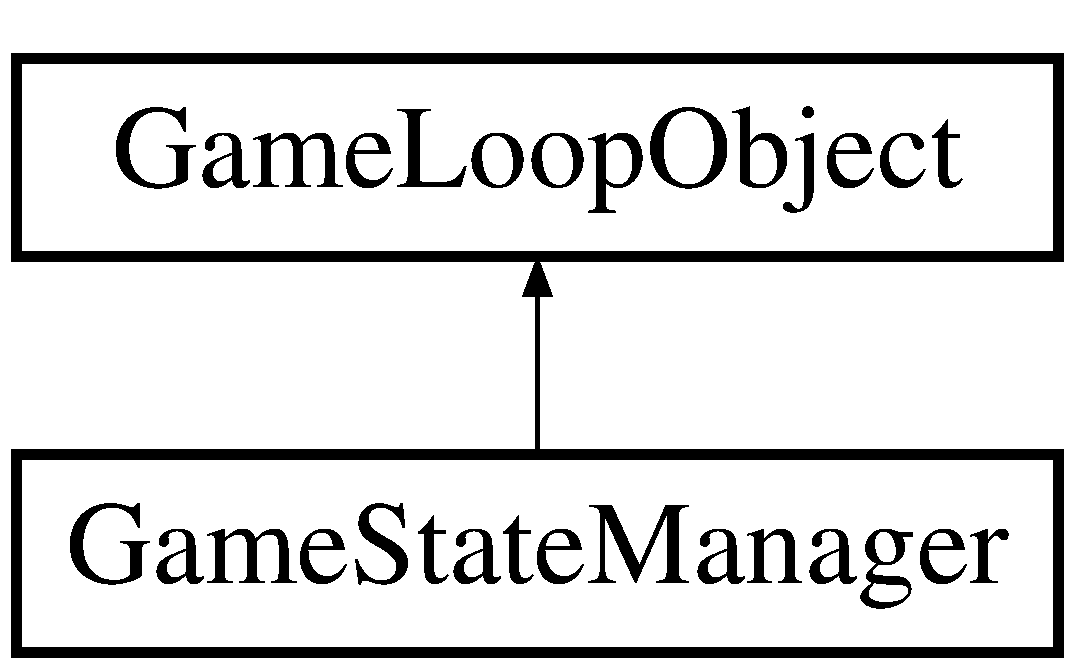
\includegraphics[height=2.000000cm]{class_game_state_manager}
\end{center}
\end{figure}
\subsection*{Public Member Functions}
\begin{DoxyCompactItemize}
\item 
\hyperlink{class_game_state_manager_aa9769dca27ad070cf5491a7f54c7d85e}{Game\+State\+Manager} ()
\begin{DoxyCompactList}\small\item\em \hyperlink{class_game_state_manager}{Game\+State\+Manager} constructor method. Sets its pointers to be empty. \end{DoxyCompactList}\item 
void \hyperlink{class_game_state_manager_a0497e8b8e72c454f1cef26defb20c05b}{Add\+Game\+State} (std\+::string name, \hyperlink{class_game_state}{Game\+State} $\ast$state)
\begin{DoxyCompactList}\small\item\em Method used to store new gamestates into the manager\textquotesingle{}s list, to be used. \end{DoxyCompactList}\item 
void \hyperlink{class_game_state_manager_af8cbaea21729562478195de2d2c3e3a2}{Refresh\+Game\+State} (std\+::string name, \hyperlink{class_game_state}{Game\+State} $\ast$state)
\begin{DoxyCompactList}\small\item\em Method used to reload a gamestate by readding it to the manager\textquotesingle{}s list. \end{DoxyCompactList}\item 
void \hyperlink{class_game_state_manager_a5f1166e0a2f868ce324f69cffc4af867}{Set\+Next} (std\+::string name)
\begin{DoxyCompactList}\small\item\em Method used to set the next gamestate. \end{DoxyCompactList}\item 
void \hyperlink{class_game_state_manager_af714c9a04112cf1b0738e8b6caec1022}{Switch\+State} ()
\begin{DoxyCompactList}\small\item\em Method used to switch to the next state, that was previously set. \end{DoxyCompactList}\item 
void \hyperlink{class_game_state_manager_a6546ed46ea23d9a9206c7d540e8b3b3b}{Handle\+Input} ()
\begin{DoxyCompactList}\small\item\em Calls the currently selected gamestate\textquotesingle{}s Handle\+Input method. \end{DoxyCompactList}\item 
void \hyperlink{class_game_state_manager_a749124e1fcaaa5eae4578bf8e3f6e4d5}{Update} ()
\begin{DoxyCompactList}\small\item\em Calls the currently selected gamestate\textquotesingle{}s Update method. \end{DoxyCompactList}\item 
void \hyperlink{class_game_state_manager_a4d42ae9f3b8c87f420fc79fd716e0c17}{Draw} (sf\+::\+Render\+Window \&window)
\begin{DoxyCompactList}\small\item\em Calls the currently selected gamestate\textquotesingle{}s Draw method. \end{DoxyCompactList}\item 
void \hyperlink{class_game_state_manager_ab92faa645a6049828d6a4048779e0aee}{Reset} ()
\begin{DoxyCompactList}\small\item\em Calls the currently selected gamestate\textquotesingle{}s Reset method. \end{DoxyCompactList}\end{DoxyCompactItemize}
\subsection*{Public Attributes}
\begin{DoxyCompactItemize}
\item 
std\+::map$<$ std\+::string, \hyperlink{class_game_state}{Game\+State} $\ast$ $>$ \hyperlink{class_game_state_manager_a6caa17360f7be10f8703decca4bc0421}{game\+States} \{\}
\end{DoxyCompactItemize}


\subsection{Detailed Description}
The game\textquotesingle{}s \hyperlink{class_game_state_manager}{Game\+State\+Manager}. Handles most of the game loop. 

The \hyperlink{class_game_state_manager}{Game\+State\+Manager} is created once and holds a list (map actually) of all gamestates the game has. All gamestates are loaded on startup, which is not memory effici�nt. The \hyperlink{class_game_state_manager}{Game\+State\+Manager} calls its current gamestate\textquotesingle{}s update, draw and handleinput methods 60 times per second during the game loop. When switching gamestates, the new gamestate is first set with the Set\+Next method and eventually switched to with the Switch\+State method. For this, this class holds two \hyperlink{class_game_state}{Game\+State} pointers that point to gamestates in the list. One to the current state that is now running and one to the next state to which the \hyperlink{class_game_state_manager}{Game\+State\+Manager} will soon switch. As soon as the \hyperlink{class_game_state_manager}{Game\+State\+Manager} is made, gamestates should be added to it using the Add\+Game\+State method and immediately after, the Set\+Next and Switch\+State methods should be called. 

Definition at line 25 of file Game\+State\+Manager.\+hpp.



\subsection{Constructor \& Destructor Documentation}
\mbox{\Hypertarget{class_game_state_manager_aa9769dca27ad070cf5491a7f54c7d85e}\label{class_game_state_manager_aa9769dca27ad070cf5491a7f54c7d85e}} 
\index{Game\+State\+Manager@{Game\+State\+Manager}!Game\+State\+Manager@{Game\+State\+Manager}}
\index{Game\+State\+Manager@{Game\+State\+Manager}!Game\+State\+Manager@{Game\+State\+Manager}}
\subsubsection{\texorpdfstring{Game\+State\+Manager()}{GameStateManager()}}
{\footnotesize\ttfamily Game\+State\+Manager\+::\+Game\+State\+Manager (\begin{DoxyParamCaption}{ }\end{DoxyParamCaption})}



\hyperlink{class_game_state_manager}{Game\+State\+Manager} constructor method. Sets its pointers to be empty. 

When the \hyperlink{class_game_state_manager}{Game\+State\+Manager} is made, the game\+States list is empty and its current state and next state pointers will be initialized to be empty. 

Definition at line 5 of file Game\+State\+Manager.\+cpp.



\subsection{Member Function Documentation}
\mbox{\Hypertarget{class_game_state_manager_a0497e8b8e72c454f1cef26defb20c05b}\label{class_game_state_manager_a0497e8b8e72c454f1cef26defb20c05b}} 
\index{Game\+State\+Manager@{Game\+State\+Manager}!Add\+Game\+State@{Add\+Game\+State}}
\index{Add\+Game\+State@{Add\+Game\+State}!Game\+State\+Manager@{Game\+State\+Manager}}
\subsubsection{\texorpdfstring{Add\+Game\+State()}{AddGameState()}}
{\footnotesize\ttfamily void Game\+State\+Manager\+::\+Add\+Game\+State (\begin{DoxyParamCaption}\item[{std\+::string}]{name,  }\item[{\hyperlink{class_game_state}{Game\+State} $\ast$}]{state }\end{DoxyParamCaption})}



Method used to store new gamestates into the manager\textquotesingle{}s list, to be used. 

This method asks for a string and a gamestate and then stores the gamestate using the chosen string as its key. 

Definition at line 10 of file Game\+State\+Manager.\+cpp.

\mbox{\Hypertarget{class_game_state_manager_a4d42ae9f3b8c87f420fc79fd716e0c17}\label{class_game_state_manager_a4d42ae9f3b8c87f420fc79fd716e0c17}} 
\index{Game\+State\+Manager@{Game\+State\+Manager}!Draw@{Draw}}
\index{Draw@{Draw}!Game\+State\+Manager@{Game\+State\+Manager}}
\subsubsection{\texorpdfstring{Draw()}{Draw()}}
{\footnotesize\ttfamily void Game\+State\+Manager\+::\+Draw (\begin{DoxyParamCaption}\item[{sf\+::\+Render\+Window \&}]{window }\end{DoxyParamCaption})\hspace{0.3cm}{\ttfamily [virtual]}}



Calls the currently selected gamestate\textquotesingle{}s Draw method. 

This method should be called in each iteration of the game loop. It will then proceed to call the currently selected gamestate\textquotesingle{}s Draw method and do only that. 

Reimplemented from \hyperlink{class_game_loop_object_a0572a88e5b98fa8a41078260d152202d}{Game\+Loop\+Object}.



Definition at line 65 of file Game\+State\+Manager.\+cpp.

\mbox{\Hypertarget{class_game_state_manager_a6546ed46ea23d9a9206c7d540e8b3b3b}\label{class_game_state_manager_a6546ed46ea23d9a9206c7d540e8b3b3b}} 
\index{Game\+State\+Manager@{Game\+State\+Manager}!Handle\+Input@{Handle\+Input}}
\index{Handle\+Input@{Handle\+Input}!Game\+State\+Manager@{Game\+State\+Manager}}
\subsubsection{\texorpdfstring{Handle\+Input()}{HandleInput()}}
{\footnotesize\ttfamily void Game\+State\+Manager\+::\+Handle\+Input (\begin{DoxyParamCaption}{ }\end{DoxyParamCaption})\hspace{0.3cm}{\ttfamily [virtual]}}



Calls the currently selected gamestate\textquotesingle{}s Handle\+Input method. 

This method should be called in each iteration of the game loop. It will then proceed to call the currently selected gamestate\textquotesingle{}s Handle\+Input method and do only that. 

Reimplemented from \hyperlink{class_game_loop_object_aecab111d504b7f4590045ca7c83a36de}{Game\+Loop\+Object}.



Definition at line 55 of file Game\+State\+Manager.\+cpp.

\mbox{\Hypertarget{class_game_state_manager_af8cbaea21729562478195de2d2c3e3a2}\label{class_game_state_manager_af8cbaea21729562478195de2d2c3e3a2}} 
\index{Game\+State\+Manager@{Game\+State\+Manager}!Refresh\+Game\+State@{Refresh\+Game\+State}}
\index{Refresh\+Game\+State@{Refresh\+Game\+State}!Game\+State\+Manager@{Game\+State\+Manager}}
\subsubsection{\texorpdfstring{Refresh\+Game\+State()}{RefreshGameState()}}
{\footnotesize\ttfamily void Game\+State\+Manager\+::\+Refresh\+Game\+State (\begin{DoxyParamCaption}\item[{std\+::string}]{name,  }\item[{\hyperlink{class_game_state}{Game\+State} $\ast$}]{state }\end{DoxyParamCaption})}



Method used to reload a gamestate by readding it to the manager\textquotesingle{}s list. 

This method asks for a string and a gamestate and then checks if the submitted name exists in the manager\textquotesingle{}s list. If it does, it is reloaded, else nothing happens. 

Definition at line 21 of file Game\+State\+Manager.\+cpp.

\mbox{\Hypertarget{class_game_state_manager_ab92faa645a6049828d6a4048779e0aee}\label{class_game_state_manager_ab92faa645a6049828d6a4048779e0aee}} 
\index{Game\+State\+Manager@{Game\+State\+Manager}!Reset@{Reset}}
\index{Reset@{Reset}!Game\+State\+Manager@{Game\+State\+Manager}}
\subsubsection{\texorpdfstring{Reset()}{Reset()}}
{\footnotesize\ttfamily void Game\+State\+Manager\+::\+Reset (\begin{DoxyParamCaption}{ }\end{DoxyParamCaption})\hspace{0.3cm}{\ttfamily [virtual]}}



Calls the currently selected gamestate\textquotesingle{}s Reset method. 

This method will call the currently selected gamestate\textquotesingle{}s Reset method and do only that. 

Reimplemented from \hyperlink{class_game_loop_object_af61e973be170cb9437a5b7d9ecd6ef53}{Game\+Loop\+Object}.



Definition at line 70 of file Game\+State\+Manager.\+cpp.

\mbox{\Hypertarget{class_game_state_manager_a5f1166e0a2f868ce324f69cffc4af867}\label{class_game_state_manager_a5f1166e0a2f868ce324f69cffc4af867}} 
\index{Game\+State\+Manager@{Game\+State\+Manager}!Set\+Next@{Set\+Next}}
\index{Set\+Next@{Set\+Next}!Game\+State\+Manager@{Game\+State\+Manager}}
\subsubsection{\texorpdfstring{Set\+Next()}{SetNext()}}
{\footnotesize\ttfamily void Game\+State\+Manager\+::\+Set\+Next (\begin{DoxyParamCaption}\item[{std\+::string}]{name }\end{DoxyParamCaption})}



Method used to set the next gamestate. 

This method asks for a gamestate name and then checks if it exists in the \hyperlink{class_game_state_manager}{Game\+State\+Manager}\textquotesingle{}s list of gamestates. If so, the inserted state is set. If not, nothing happens. 

Definition at line 33 of file Game\+State\+Manager.\+cpp.

\mbox{\Hypertarget{class_game_state_manager_af714c9a04112cf1b0738e8b6caec1022}\label{class_game_state_manager_af714c9a04112cf1b0738e8b6caec1022}} 
\index{Game\+State\+Manager@{Game\+State\+Manager}!Switch\+State@{Switch\+State}}
\index{Switch\+State@{Switch\+State}!Game\+State\+Manager@{Game\+State\+Manager}}
\subsubsection{\texorpdfstring{Switch\+State()}{SwitchState()}}
{\footnotesize\ttfamily void Game\+State\+Manager\+::\+Switch\+State (\begin{DoxyParamCaption}{ }\end{DoxyParamCaption})}



Method used to switch to the next state, that was previously set. 

This method checks if a new state has been set. If not, nothing happens. But if a next state has been previously set, the \hyperlink{class_game_state_manager}{Game\+State\+Manager} will then proceed to switch the current state to the next state, which from then on will be run in the game loop. The \textquotesingle{}next\+State\textquotesingle{} pointer will be cleared and stay empty until a new state is set. 

Definition at line 45 of file Game\+State\+Manager.\+cpp.

\mbox{\Hypertarget{class_game_state_manager_a749124e1fcaaa5eae4578bf8e3f6e4d5}\label{class_game_state_manager_a749124e1fcaaa5eae4578bf8e3f6e4d5}} 
\index{Game\+State\+Manager@{Game\+State\+Manager}!Update@{Update}}
\index{Update@{Update}!Game\+State\+Manager@{Game\+State\+Manager}}
\subsubsection{\texorpdfstring{Update()}{Update()}}
{\footnotesize\ttfamily void Game\+State\+Manager\+::\+Update (\begin{DoxyParamCaption}{ }\end{DoxyParamCaption})\hspace{0.3cm}{\ttfamily [virtual]}}



Calls the currently selected gamestate\textquotesingle{}s Update method. 

This method should be called in each iteration of the game loop. It will then proceed to call the currently selected gamestate\textquotesingle{}s Update method and do only that. 

Reimplemented from \hyperlink{class_game_loop_object_ae36a15981f1dd3f3bea6050473490349}{Game\+Loop\+Object}.



Definition at line 60 of file Game\+State\+Manager.\+cpp.



\subsection{Member Data Documentation}
\mbox{\Hypertarget{class_game_state_manager_a6caa17360f7be10f8703decca4bc0421}\label{class_game_state_manager_a6caa17360f7be10f8703decca4bc0421}} 
\index{Game\+State\+Manager@{Game\+State\+Manager}!game\+States@{game\+States}}
\index{game\+States@{game\+States}!Game\+State\+Manager@{Game\+State\+Manager}}
\subsubsection{\texorpdfstring{game\+States}{gameStates}}
{\footnotesize\ttfamily std\+::map$<$std\+::string, \hyperlink{class_game_state}{Game\+State} $\ast$$>$ Game\+State\+Manager\+::game\+States \{\}}



Definition at line 30 of file Game\+State\+Manager.\+hpp.



The documentation for this class was generated from the following files\+:\begin{DoxyCompactItemize}
\item 
C\+:/\+Users/joost/\+Documents/\+Git\+Hub/topdown/\+Code/\+Team\+Topdown/\+Team\+Topdown/\hyperlink{_game_state_manager_8hpp}{Game\+State\+Manager.\+hpp}\item 
C\+:/\+Users/joost/\+Documents/\+Git\+Hub/topdown/\+Code/\+Team\+Topdown/\+Team\+Topdown/\hyperlink{_game_state_manager_8cpp}{Game\+State\+Manager.\+cpp}\end{DoxyCompactItemize}

\hypertarget{class_graphic}{}\section{Graphic Class Reference}
\label{class_graphic}\index{Graphic@{Graphic}}


Creates a graphic object.  




{\ttfamily \#include $<$Graphic.\+h$>$}

\subsection*{Public Member Functions}
\begin{DoxyCompactItemize}
\item 
\hyperlink{class_graphic_a83bb982f987a5c5c70e7a6134ba855ee}{Graphic} (String path, bool center\+Sprite=false)
\item 
void \hyperlink{class_graphic_ad177824925cb750fd1b2cb8ef8e40f16}{rotate} (float rotation)
\item 
void \hyperlink{class_graphic_ab19115e7bd2f656ad4939b2a412cd4d6}{set\+Position} (Vector2f pos)
\item 
void \hyperlink{class_graphic_a681124d0e87f6e8d14211195c4832880}{set\+Scale} (Vector2f scale)
\item 
void \hyperlink{class_graphic_a5b21e6698c7fab47a5e3770a8d8747d5}{draw} (Render\+Window \&w)
\item 
void \hyperlink{class_graphic_a33969eb4051f1f51c67bf2e8d0959f2d}{Set\+Sprite} (std\+::string path, bool center\+Sprite=false)
\end{DoxyCompactItemize}


\subsection{Detailed Description}
Creates a graphic object. 

Definition at line 14 of file Graphic.\+h.



\subsection{Constructor \& Destructor Documentation}
\mbox{\Hypertarget{class_graphic_a83bb982f987a5c5c70e7a6134ba855ee}\label{class_graphic_a83bb982f987a5c5c70e7a6134ba855ee}} 
\index{Graphic@{Graphic}!Graphic@{Graphic}}
\index{Graphic@{Graphic}!Graphic@{Graphic}}
\subsubsection{\texorpdfstring{Graphic()}{Graphic()}}
{\footnotesize\ttfamily Graphic\+::\+Graphic (\begin{DoxyParamCaption}\item[{String}]{path,  }\item[{bool}]{center\+Sprite = {\ttfamily false} }\end{DoxyParamCaption})}



Definition at line 4 of file Graphic.\+cpp.



\subsection{Member Function Documentation}
\mbox{\Hypertarget{class_graphic_a5b21e6698c7fab47a5e3770a8d8747d5}\label{class_graphic_a5b21e6698c7fab47a5e3770a8d8747d5}} 
\index{Graphic@{Graphic}!draw@{draw}}
\index{draw@{draw}!Graphic@{Graphic}}
\subsubsection{\texorpdfstring{draw()}{draw()}}
{\footnotesize\ttfamily void Graphic\+::draw (\begin{DoxyParamCaption}\item[{Render\+Window \&}]{w }\end{DoxyParamCaption})}

/void \hyperlink{class_graphic_a5b21e6698c7fab47a5e3770a8d8747d5}{draw(\+Render\+Window \& w)} /brief draws sprite 

Definition at line 21 of file Graphic.\+cpp.

\mbox{\Hypertarget{class_graphic_ad177824925cb750fd1b2cb8ef8e40f16}\label{class_graphic_ad177824925cb750fd1b2cb8ef8e40f16}} 
\index{Graphic@{Graphic}!rotate@{rotate}}
\index{rotate@{rotate}!Graphic@{Graphic}}
\subsubsection{\texorpdfstring{rotate()}{rotate()}}
{\footnotesize\ttfamily void Graphic\+::rotate (\begin{DoxyParamCaption}\item[{float}]{rotation }\end{DoxyParamCaption})}

/void \hyperlink{class_graphic_ad177824925cb750fd1b2cb8ef8e40f16}{rotate(float rotation)} /brief rotates sprite based on float rotation 

Definition at line 9 of file Graphic.\+cpp.

\mbox{\Hypertarget{class_graphic_ab19115e7bd2f656ad4939b2a412cd4d6}\label{class_graphic_ab19115e7bd2f656ad4939b2a412cd4d6}} 
\index{Graphic@{Graphic}!set\+Position@{set\+Position}}
\index{set\+Position@{set\+Position}!Graphic@{Graphic}}
\subsubsection{\texorpdfstring{set\+Position()}{setPosition()}}
{\footnotesize\ttfamily void Graphic\+::set\+Position (\begin{DoxyParamCaption}\item[{Vector2f}]{pos }\end{DoxyParamCaption})}

/void set\+Position /brief sets sprite position based on Vector2f pos 

Definition at line 14 of file Graphic.\+cpp.

\mbox{\Hypertarget{class_graphic_a681124d0e87f6e8d14211195c4832880}\label{class_graphic_a681124d0e87f6e8d14211195c4832880}} 
\index{Graphic@{Graphic}!set\+Scale@{set\+Scale}}
\index{set\+Scale@{set\+Scale}!Graphic@{Graphic}}
\subsubsection{\texorpdfstring{set\+Scale()}{setScale()}}
{\footnotesize\ttfamily void Graphic\+::set\+Scale (\begin{DoxyParamCaption}\item[{Vector2f}]{scale }\end{DoxyParamCaption})}

/void \hyperlink{class_graphic_a681124d0e87f6e8d14211195c4832880}{set\+Scale(\+Vector2f scale)} /brief sets sprite scale based on Vector2f scale 

Definition at line 18 of file Graphic.\+cpp.

\mbox{\Hypertarget{class_graphic_a33969eb4051f1f51c67bf2e8d0959f2d}\label{class_graphic_a33969eb4051f1f51c67bf2e8d0959f2d}} 
\index{Graphic@{Graphic}!Set\+Sprite@{Set\+Sprite}}
\index{Set\+Sprite@{Set\+Sprite}!Graphic@{Graphic}}
\subsubsection{\texorpdfstring{Set\+Sprite()}{SetSprite()}}
{\footnotesize\ttfamily void Graphic\+::\+Set\+Sprite (\begin{DoxyParamCaption}\item[{std\+::string}]{path,  }\item[{bool}]{center\+Sprite = {\ttfamily false} }\end{DoxyParamCaption})}

/void Set\+Sprite /brief sets sprite png to string path and checks a bool if sprite initial position should be centered 

Definition at line 25 of file Graphic.\+cpp.



The documentation for this class was generated from the following files\+:\begin{DoxyCompactItemize}
\item 
C\+:/\+Users/joost/\+Documents/\+Git\+Hub/topdown/\+Code/\+Team\+Topdown/\+Team\+Topdown/\hyperlink{_graphic_8h}{Graphic.\+h}\item 
C\+:/\+Users/joost/\+Documents/\+Git\+Hub/topdown/\+Code/\+Team\+Topdown/\+Team\+Topdown/\hyperlink{_graphic_8cpp}{Graphic.\+cpp}\end{DoxyCompactItemize}

\hypertarget{class_highscores_state}{}\section{Highscores\+State Class Reference}
\label{class_highscores_state}\index{Highscores\+State@{Highscores\+State}}


The gamestate that shows the (unimplemented) high scores.  




{\ttfamily \#include $<$Highscores\+State.\+hpp$>$}

Inheritance diagram for Highscores\+State\+:\begin{figure}[H]
\begin{center}
\leavevmode
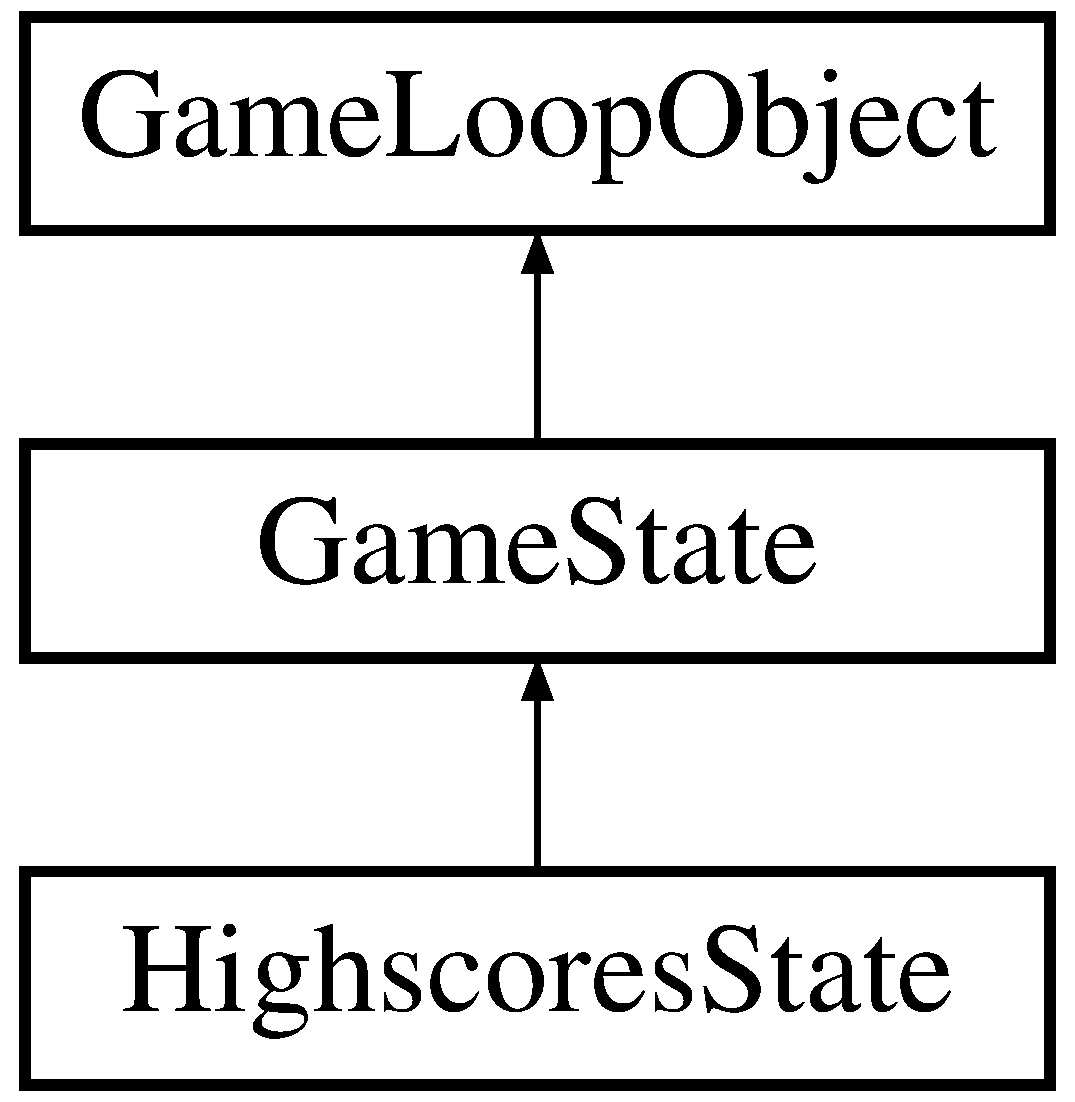
\includegraphics[height=3.000000cm]{class_highscores_state}
\end{center}
\end{figure}
\subsection*{Public Member Functions}
\begin{DoxyCompactItemize}
\item 
\hyperlink{class_highscores_state_ad01d7f96f196c29ddbdfe1827ae9b894}{Highscores\+State} (sf\+::\+Render\+Window \&window, \hyperlink{class_game_state_manager}{Game\+State\+Manager} \&gsm, \hyperlink{struct_controls_input}{Controls\+Input} \&ci)
\begin{DoxyCompactList}\small\item\em The title screen\textquotesingle{}s constructor method. \end{DoxyCompactList}\item 
void \hyperlink{class_highscores_state_aa8ce1b29acad9790ff065e5c96635c85}{Handle\+Input} ()
\begin{DoxyCompactList}\small\item\em The highscores screen\textquotesingle{}s game loop method for handling user input. \end{DoxyCompactList}\item 
void \hyperlink{class_highscores_state_a8a55079503b5bdaf205e74eb9d48dae0}{Update} ()
\begin{DoxyCompactList}\small\item\em The highscores screen\textquotesingle{}s game loop method for updating the game. \end{DoxyCompactList}\item 
void \hyperlink{class_highscores_state_a50fc2005675f2cc1740e3f9ef698bdab}{Draw} (sf\+::\+Render\+Window \&window)
\begin{DoxyCompactList}\small\item\em The title screen\textquotesingle{}s game loop method for drawing on the window. \end{DoxyCompactList}\item 
void \hyperlink{class_highscores_state_a6368de23eaf55fa1cd40cba04cbd07a0}{Reset} ()
\begin{DoxyCompactList}\small\item\em The intro state\textquotesingle{}s reset method to reset all values to default. \end{DoxyCompactList}\end{DoxyCompactItemize}


\subsection{Detailed Description}
The gamestate that shows the (unimplemented) high scores. 

This gamestate shows the highscores screen. Pressing space/enter/backspace lets the player return to the main menu. High scores are not implemented. This screen currently is a placeholder. 

Definition at line 16 of file Highscores\+State.\+hpp.



\subsection{Constructor \& Destructor Documentation}
\mbox{\Hypertarget{class_highscores_state_ad01d7f96f196c29ddbdfe1827ae9b894}\label{class_highscores_state_ad01d7f96f196c29ddbdfe1827ae9b894}} 
\index{Highscores\+State@{Highscores\+State}!Highscores\+State@{Highscores\+State}}
\index{Highscores\+State@{Highscores\+State}!Highscores\+State@{Highscores\+State}}
\subsubsection{\texorpdfstring{Highscores\+State()}{HighscoresState()}}
{\footnotesize\ttfamily Highscores\+State\+::\+Highscores\+State (\begin{DoxyParamCaption}\item[{sf\+::\+Render\+Window \&}]{window,  }\item[{\hyperlink{class_game_state_manager}{Game\+State\+Manager} \&}]{gsm,  }\item[{\hyperlink{struct_controls_input}{Controls\+Input} \&}]{ci }\end{DoxyParamCaption})}



The title screen\textquotesingle{}s constructor method. 

The title screen\textquotesingle{}s constructor requires a window to draw on, the gamestatemanager to be able to switch states and the controlsinput to read user input. 

Definition at line 5 of file Highscores\+State.\+cpp.



\subsection{Member Function Documentation}
\mbox{\Hypertarget{class_highscores_state_a50fc2005675f2cc1740e3f9ef698bdab}\label{class_highscores_state_a50fc2005675f2cc1740e3f9ef698bdab}} 
\index{Highscores\+State@{Highscores\+State}!Draw@{Draw}}
\index{Draw@{Draw}!Highscores\+State@{Highscores\+State}}
\subsubsection{\texorpdfstring{Draw()}{Draw()}}
{\footnotesize\ttfamily void Highscores\+State\+::\+Draw (\begin{DoxyParamCaption}\item[{sf\+::\+Render\+Window \&}]{window }\end{DoxyParamCaption})\hspace{0.3cm}{\ttfamily [virtual]}}



The title screen\textquotesingle{}s game loop method for drawing on the window. 

Draws the placeholder background and text on the screen. 

Reimplemented from \hyperlink{class_game_state_a8741c5c696c6c366beb4b845c08c3cf8}{Game\+State}.



Definition at line 35 of file Highscores\+State.\+cpp.

\mbox{\Hypertarget{class_highscores_state_aa8ce1b29acad9790ff065e5c96635c85}\label{class_highscores_state_aa8ce1b29acad9790ff065e5c96635c85}} 
\index{Highscores\+State@{Highscores\+State}!Handle\+Input@{Handle\+Input}}
\index{Handle\+Input@{Handle\+Input}!Highscores\+State@{Highscores\+State}}
\subsubsection{\texorpdfstring{Handle\+Input()}{HandleInput()}}
{\footnotesize\ttfamily void Highscores\+State\+::\+Handle\+Input (\begin{DoxyParamCaption}{ }\end{DoxyParamCaption})\hspace{0.3cm}{\ttfamily [virtual]}}



The highscores screen\textquotesingle{}s game loop method for handling user input. 

This method handles all user input related to this gamestate. Pressing space/enter/backspace lets the player return to the main menu. 

Reimplemented from \hyperlink{class_game_state_a8bce2828cee99ae7c07322804531fd01}{Game\+State}.



Definition at line 22 of file Highscores\+State.\+cpp.

\mbox{\Hypertarget{class_highscores_state_a6368de23eaf55fa1cd40cba04cbd07a0}\label{class_highscores_state_a6368de23eaf55fa1cd40cba04cbd07a0}} 
\index{Highscores\+State@{Highscores\+State}!Reset@{Reset}}
\index{Reset@{Reset}!Highscores\+State@{Highscores\+State}}
\subsubsection{\texorpdfstring{Reset()}{Reset()}}
{\footnotesize\ttfamily void Highscores\+State\+::\+Reset (\begin{DoxyParamCaption}{ }\end{DoxyParamCaption})\hspace{0.3cm}{\ttfamily [virtual]}}



The intro state\textquotesingle{}s reset method to reset all values to default. 

Doesn\textquotesingle{}t do anything. 

Reimplemented from \hyperlink{class_game_state_a46ac6317883dff0eba4f8f305af6b6bb}{Game\+State}.



Definition at line 43 of file Highscores\+State.\+cpp.

\mbox{\Hypertarget{class_highscores_state_a8a55079503b5bdaf205e74eb9d48dae0}\label{class_highscores_state_a8a55079503b5bdaf205e74eb9d48dae0}} 
\index{Highscores\+State@{Highscores\+State}!Update@{Update}}
\index{Update@{Update}!Highscores\+State@{Highscores\+State}}
\subsubsection{\texorpdfstring{Update()}{Update()}}
{\footnotesize\ttfamily void Highscores\+State\+::\+Update (\begin{DoxyParamCaption}{ }\end{DoxyParamCaption})\hspace{0.3cm}{\ttfamily [virtual]}}



The highscores screen\textquotesingle{}s game loop method for updating the game. 

Currently only checks if a gamestate switch should be executed. 

Reimplemented from \hyperlink{class_game_state_a5be51b634f95bc6e57066ad6931aa18b}{Game\+State}.



Definition at line 30 of file Highscores\+State.\+cpp.



The documentation for this class was generated from the following files\+:\begin{DoxyCompactItemize}
\item 
C\+:/\+Users/joost/\+Documents/\+Git\+Hub/topdown/\+Code/\+Team\+Topdown/\+Team\+Topdown/\hyperlink{_highscores_state_8hpp}{Highscores\+State.\+hpp}\item 
C\+:/\+Users/joost/\+Documents/\+Git\+Hub/topdown/\+Code/\+Team\+Topdown/\+Team\+Topdown/\hyperlink{_highscores_state_8cpp}{Highscores\+State.\+cpp}\end{DoxyCompactItemize}

\hypertarget{class_hud}{}\section{Hud Class Reference}
\label{class_hud}\index{Hud@{Hud}}


Creates a hud overlay with the following\+:  




{\ttfamily \#include $<$Hud.\+h$>$}

\subsection*{Public Member Functions}
\begin{DoxyCompactItemize}
\item 
\hyperlink{class_hud_a70b69eaa00542d46595069dafc768913}{Hud} (\hyperlink{struct_player_stats}{Player\+Stats} \&stats=\hyperlink{struct_player_stats}{Player\+Stats}())
\item 
\hyperlink{class_hud_a2fbb662bbc70f646e081f9206a879b66}{$\sim$\+Hud} ()
\item 
void \hyperlink{class_hud_af9ec2f89bcc54651d2413aeb5cbc53b3}{update} ()
\begin{DoxyCompactList}\small\item\em updates the hud \end{DoxyCompactList}\item 
void \hyperlink{class_hud_a4140716cb23f7cdd8436d7ebd77a85ab}{display\+Ammo} ()
\begin{DoxyCompactList}\small\item\em initial draw and set the current ammo display to the max bullets the player can have \end{DoxyCompactList}\item 
void \hyperlink{class_hud_a9fdcb19f4fd4d323dc7b3dd09bd85a08}{update\+Ammo} ()
\begin{DoxyCompactList}\small\item\em updates the current displayed ammo \end{DoxyCompactList}\item 
void \hyperlink{class_hud_a88e6f0b9be11e3aa59b7b4ab14d98ffa}{draw\+Ammo} (Render\+Window \&w)
\begin{DoxyCompactList}\small\item\em draws the ammo sprites \end{DoxyCompactList}\item 
void \hyperlink{class_hud_ad5832e2899c6b4606ce4229247fd7f9e}{draw} (Render\+Window \&w)
\begin{DoxyCompactList}\small\item\em draws the following sprites on Render\+Window \& w \end{DoxyCompactList}\item 
void \hyperlink{class_hud_accfaddbefc4b7ba1ecf64d3b32af2d24}{create\+Pop\+Up} (int total\+Ammo\+Added, Vector2f position)
\begin{DoxyCompactList}\small\item\em creates a popup to be displayed, floating upward on a position \end{DoxyCompactList}\item 
void \hyperlink{class_hud_a6c8effbe343872e65e9d02f0509be0d6}{delete\+Pop\+Up} (std\+::vector$<$ Pop\+Up $\ast$$>$\+::iterator \&pop\+Up\+It)
\begin{DoxyCompactList}\small\item\em deletes a popup to be displayed, floating upward on a position \end{DoxyCompactList}\item 
void \hyperlink{class_hud_a2404ab603f0646b3b320616e7dfbc957}{reset\+Time} ()
\end{DoxyCompactItemize}


\subsection{Detailed Description}
Creates a hud overlay with the following\+: 


\begin{DoxyItemize}
\item Ammo counters
\item font
\item game time
\item player stamina
\item graphical fluff 
\end{DoxyItemize}

Definition at line 18 of file Hud.\+h.



\subsection{Constructor \& Destructor Documentation}
\mbox{\Hypertarget{class_hud_a70b69eaa00542d46595069dafc768913}\label{class_hud_a70b69eaa00542d46595069dafc768913}} 
\index{Hud@{Hud}!Hud@{Hud}}
\index{Hud@{Hud}!Hud@{Hud}}
\subsubsection{\texorpdfstring{Hud()}{Hud()}}
{\footnotesize\ttfamily Hud\+::\+Hud (\begin{DoxyParamCaption}\item[{\hyperlink{struct_player_stats}{Player\+Stats} \&}]{stats = {\ttfamily \hyperlink{struct_player_stats}{Player\+Stats}()} }\end{DoxyParamCaption})}



Definition at line 5 of file Hud.\+cpp.

\mbox{\Hypertarget{class_hud_a2fbb662bbc70f646e081f9206a879b66}\label{class_hud_a2fbb662bbc70f646e081f9206a879b66}} 
\index{Hud@{Hud}!````~Hud@{$\sim$\+Hud}}
\index{````~Hud@{$\sim$\+Hud}!Hud@{Hud}}
\subsubsection{\texorpdfstring{$\sim$\+Hud()}{~Hud()}}
{\footnotesize\ttfamily Hud\+::$\sim$\+Hud (\begin{DoxyParamCaption}{ }\end{DoxyParamCaption})}



Definition at line 19 of file Hud.\+cpp.



\subsection{Member Function Documentation}
\mbox{\Hypertarget{class_hud_accfaddbefc4b7ba1ecf64d3b32af2d24}\label{class_hud_accfaddbefc4b7ba1ecf64d3b32af2d24}} 
\index{Hud@{Hud}!create\+Pop\+Up@{create\+Pop\+Up}}
\index{create\+Pop\+Up@{create\+Pop\+Up}!Hud@{Hud}}
\subsubsection{\texorpdfstring{create\+Pop\+Up()}{createPopUp()}}
{\footnotesize\ttfamily void Hud\+::create\+Pop\+Up (\begin{DoxyParamCaption}\item[{int}]{total\+Ammo\+Added,  }\item[{Vector2f}]{position }\end{DoxyParamCaption})}



creates a popup to be displayed, floating upward on a position 

create\+Pop\+Up 

Definition at line 130 of file Hud.\+cpp.

\mbox{\Hypertarget{class_hud_a6c8effbe343872e65e9d02f0509be0d6}\label{class_hud_a6c8effbe343872e65e9d02f0509be0d6}} 
\index{Hud@{Hud}!delete\+Pop\+Up@{delete\+Pop\+Up}}
\index{delete\+Pop\+Up@{delete\+Pop\+Up}!Hud@{Hud}}
\subsubsection{\texorpdfstring{delete\+Pop\+Up()}{deletePopUp()}}
{\footnotesize\ttfamily void Hud\+::delete\+Pop\+Up (\begin{DoxyParamCaption}\item[{std\+::vector$<$ Pop\+Up $\ast$$>$\+::iterator \&}]{pop\+Up\+It }\end{DoxyParamCaption})}



deletes a popup to be displayed, floating upward on a position 

delete\+Pop\+Up 

Definition at line 113 of file Hud.\+cpp.

\mbox{\Hypertarget{class_hud_a4140716cb23f7cdd8436d7ebd77a85ab}\label{class_hud_a4140716cb23f7cdd8436d7ebd77a85ab}} 
\index{Hud@{Hud}!display\+Ammo@{display\+Ammo}}
\index{display\+Ammo@{display\+Ammo}!Hud@{Hud}}
\subsubsection{\texorpdfstring{display\+Ammo()}{displayAmmo()}}
{\footnotesize\ttfamily void Hud\+::display\+Ammo (\begin{DoxyParamCaption}{ }\end{DoxyParamCaption})}



initial draw and set the current ammo display to the max bullets the player can have 

\hyperlink{class_hud_a4140716cb23f7cdd8436d7ebd77a85ab}{display\+Ammo()} 

Definition at line 23 of file Hud.\+cpp.

\mbox{\Hypertarget{class_hud_ad5832e2899c6b4606ce4229247fd7f9e}\label{class_hud_ad5832e2899c6b4606ce4229247fd7f9e}} 
\index{Hud@{Hud}!draw@{draw}}
\index{draw@{draw}!Hud@{Hud}}
\subsubsection{\texorpdfstring{draw()}{draw()}}
{\footnotesize\ttfamily void Hud\+::draw (\begin{DoxyParamCaption}\item[{Render\+Window \&}]{w }\end{DoxyParamCaption})}



draws the following sprites on Render\+Window \& w 

\hyperlink{class_hud_ad5832e2899c6b4606ce4229247fd7f9e}{draw()} 

Definition at line 117 of file Hud.\+cpp.

\mbox{\Hypertarget{class_hud_a88e6f0b9be11e3aa59b7b4ab14d98ffa}\label{class_hud_a88e6f0b9be11e3aa59b7b4ab14d98ffa}} 
\index{Hud@{Hud}!draw\+Ammo@{draw\+Ammo}}
\index{draw\+Ammo@{draw\+Ammo}!Hud@{Hud}}
\subsubsection{\texorpdfstring{draw\+Ammo()}{drawAmmo()}}
{\footnotesize\ttfamily void Hud\+::draw\+Ammo (\begin{DoxyParamCaption}\item[{Render\+Window \&}]{w }\end{DoxyParamCaption})}



draws the ammo sprites 

\hyperlink{class_hud_a88e6f0b9be11e3aa59b7b4ab14d98ffa}{draw\+Ammo()} 

Definition at line 62 of file Hud.\+cpp.

\mbox{\Hypertarget{class_hud_a2404ab603f0646b3b320616e7dfbc957}\label{class_hud_a2404ab603f0646b3b320616e7dfbc957}} 
\index{Hud@{Hud}!reset\+Time@{reset\+Time}}
\index{reset\+Time@{reset\+Time}!Hud@{Hud}}
\subsubsection{\texorpdfstring{reset\+Time()}{resetTime()}}
{\footnotesize\ttfamily void Hud\+::reset\+Time (\begin{DoxyParamCaption}{ }\end{DoxyParamCaption})}



Definition at line 29 of file Hud.\+cpp.

\mbox{\Hypertarget{class_hud_af9ec2f89bcc54651d2413aeb5cbc53b3}\label{class_hud_af9ec2f89bcc54651d2413aeb5cbc53b3}} 
\index{Hud@{Hud}!update@{update}}
\index{update@{update}!Hud@{Hud}}
\subsubsection{\texorpdfstring{update()}{update()}}
{\footnotesize\ttfamily void Hud\+::update (\begin{DoxyParamCaption}{ }\end{DoxyParamCaption})}



updates the hud 

\hyperlink{class_hud_af9ec2f89bcc54651d2413aeb5cbc53b3}{update()} 

Definition at line 69 of file Hud.\+cpp.

\mbox{\Hypertarget{class_hud_a9fdcb19f4fd4d323dc7b3dd09bd85a08}\label{class_hud_a9fdcb19f4fd4d323dc7b3dd09bd85a08}} 
\index{Hud@{Hud}!update\+Ammo@{update\+Ammo}}
\index{update\+Ammo@{update\+Ammo}!Hud@{Hud}}
\subsubsection{\texorpdfstring{update\+Ammo()}{updateAmmo()}}
{\footnotesize\ttfamily void Hud\+::update\+Ammo (\begin{DoxyParamCaption}{ }\end{DoxyParamCaption})}



updates the current displayed ammo 

\hyperlink{class_hud_a9fdcb19f4fd4d323dc7b3dd09bd85a08}{update\+Ammo()} 

Definition at line 34 of file Hud.\+cpp.



The documentation for this class was generated from the following files\+:\begin{DoxyCompactItemize}
\item 
C\+:/\+Users/joost/\+Documents/\+Git\+Hub/topdown/\+Code/\+Team\+Topdown/\+Team\+Topdown/\hyperlink{_hud_8h}{Hud.\+h}\item 
C\+:/\+Users/joost/\+Documents/\+Git\+Hub/topdown/\+Code/\+Team\+Topdown/\+Team\+Topdown/\hyperlink{_hud_8cpp}{Hud.\+cpp}\end{DoxyCompactItemize}

\hypertarget{class_item}{}\section{Item Class Reference}
\label{class_item}\index{Item@{Item}}


\hyperlink{class_item}{Item} is a entity that can modify the stats.  




{\ttfamily \#include $<$Item.\+h$>$}

Inheritance diagram for Item\+:\begin{figure}[H]
\begin{center}
\leavevmode
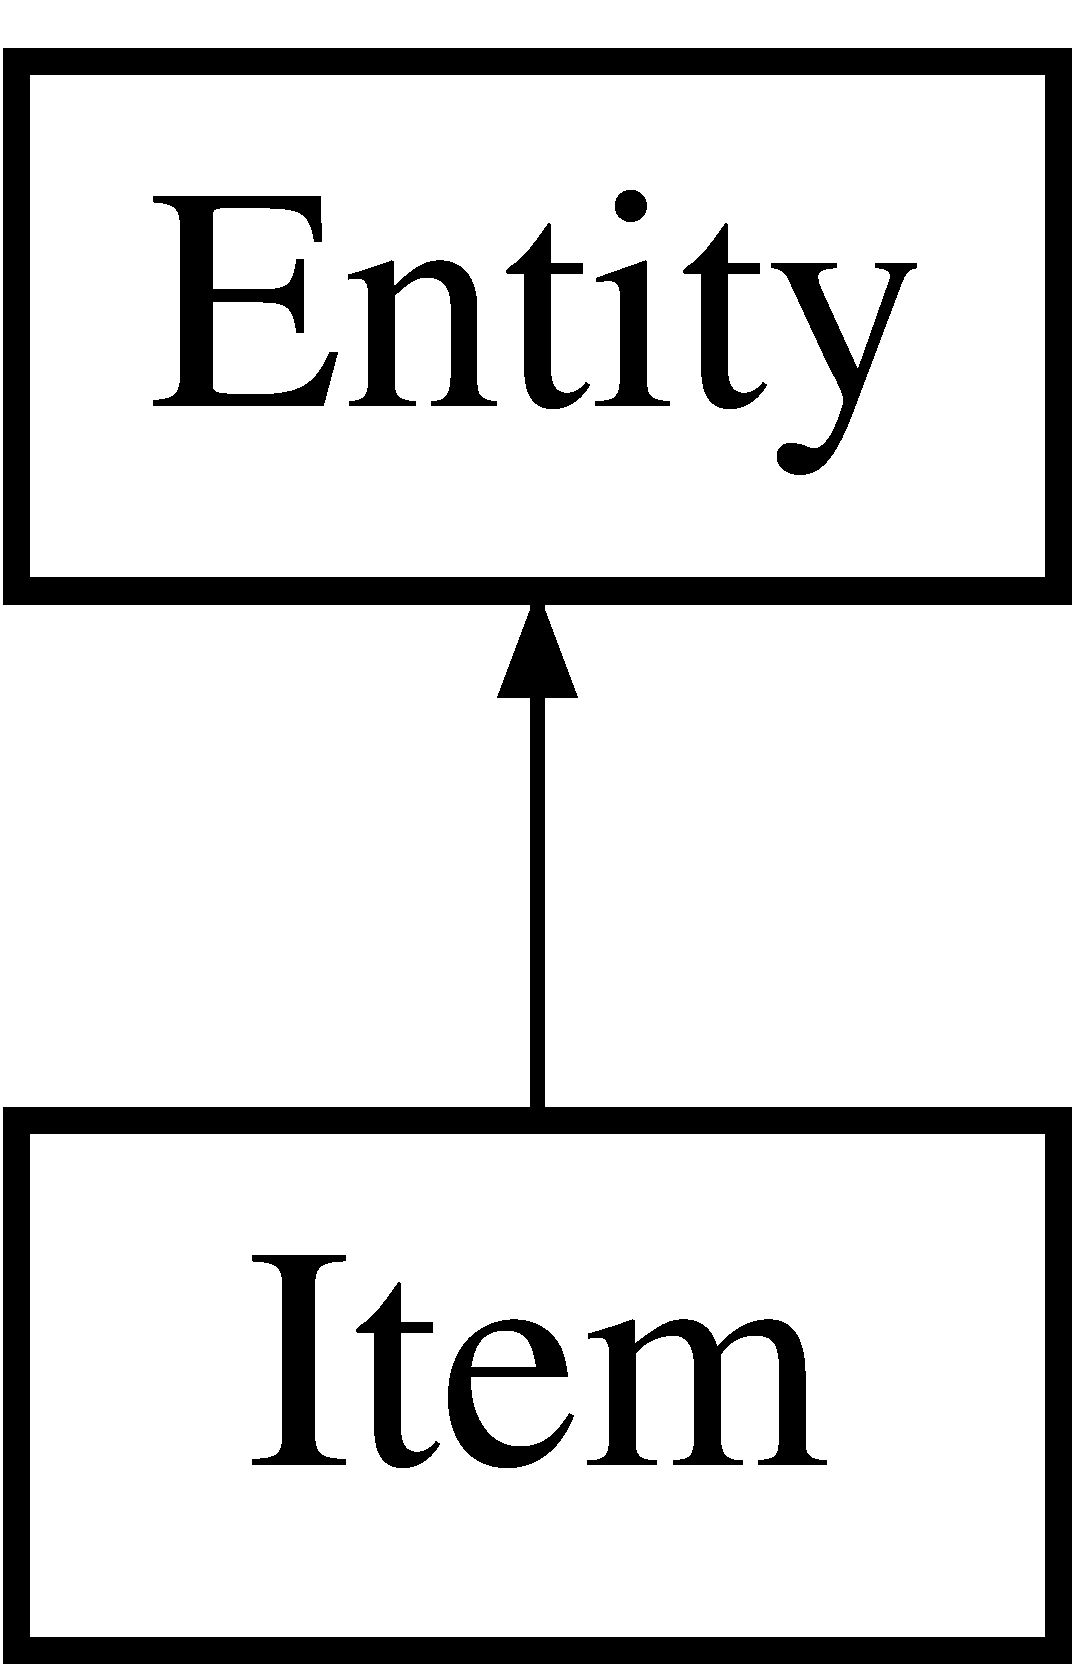
\includegraphics[height=2.000000cm]{class_item}
\end{center}
\end{figure}
\subsection*{Public Member Functions}
\begin{DoxyCompactItemize}
\item 
\hyperlink{class_item_a951b1f5cf04cf8d9ecfdae8553508f0a}{Item} (sf\+::\+Vector2f pos, sf\+::\+Vector2f \hyperlink{class_entity_ae9a0a364c85f91ade5088b3610131417}{size}, int \hyperlink{class_item_a621a125c6d736a8d44a27129fba48068}{ammo}, int \hyperlink{class_item_a5ee3cebbf90b766991c74d09bd5d12bd}{energy})
\item 
void \hyperlink{class_item_a2ec323b2001bee948fa560ee8ee48067}{draw} (sf\+::\+Render\+Window \&window) override
\item 
void \hyperlink{class_item_a149c95695cc750a3f2de14eb4ed6ef21}{pick\+Up} (\hyperlink{struct_player_stats}{Player\+Stats} \&stats)
\end{DoxyCompactItemize}
\subsection*{Public Attributes}
\begin{DoxyCompactItemize}
\item 
int \hyperlink{class_item_a621a125c6d736a8d44a27129fba48068}{ammo}
\item 
int \hyperlink{class_item_a5ee3cebbf90b766991c74d09bd5d12bd}{energy}
\end{DoxyCompactItemize}
\subsection*{Additional Inherited Members}


\subsection{Detailed Description}
\hyperlink{class_item}{Item} is a entity that can modify the stats. 

Contains the item graphic and overrides the necessary functions from \hyperlink{class_entity}{Entity}. The item contains ammo and energy that will be added when it{\ttfamily s picked up. Energy isn}t used in the end game beacuse we diced not to use it at last minute. 

Definition at line 20 of file Item.\+h.



\subsection{Constructor \& Destructor Documentation}
\mbox{\Hypertarget{class_item_a951b1f5cf04cf8d9ecfdae8553508f0a}\label{class_item_a951b1f5cf04cf8d9ecfdae8553508f0a}} 
\index{Item@{Item}!Item@{Item}}
\index{Item@{Item}!Item@{Item}}
\subsubsection{\texorpdfstring{Item()}{Item()}}
{\footnotesize\ttfamily Item\+::\+Item (\begin{DoxyParamCaption}\item[{sf\+::\+Vector2f}]{pos,  }\item[{sf\+::\+Vector2f}]{size,  }\item[{int}]{ammo,  }\item[{int}]{energy }\end{DoxyParamCaption})}



Definition at line 5 of file Item.\+cpp.



\subsection{Member Function Documentation}
\mbox{\Hypertarget{class_item_a2ec323b2001bee948fa560ee8ee48067}\label{class_item_a2ec323b2001bee948fa560ee8ee48067}} 
\index{Item@{Item}!draw@{draw}}
\index{draw@{draw}!Item@{Item}}
\subsubsection{\texorpdfstring{draw()}{draw()}}
{\footnotesize\ttfamily void Item\+::draw (\begin{DoxyParamCaption}\item[{sf\+::\+Render\+Window \&}]{window }\end{DoxyParamCaption})\hspace{0.3cm}{\ttfamily [override]}}

Draw item on window 

Definition at line 17 of file Item.\+cpp.

\mbox{\Hypertarget{class_item_a149c95695cc750a3f2de14eb4ed6ef21}\label{class_item_a149c95695cc750a3f2de14eb4ed6ef21}} 
\index{Item@{Item}!pick\+Up@{pick\+Up}}
\index{pick\+Up@{pick\+Up}!Item@{Item}}
\subsubsection{\texorpdfstring{pick\+Up()}{pickUp()}}
{\footnotesize\ttfamily void Item\+::pick\+Up (\begin{DoxyParamCaption}\item[{\hyperlink{struct_player_stats}{Player\+Stats} \&}]{stats }\end{DoxyParamCaption})}

ads ammo and energy to the player stats 

Definition at line 12 of file Item.\+cpp.



\subsection{Member Data Documentation}
\mbox{\Hypertarget{class_item_a621a125c6d736a8d44a27129fba48068}\label{class_item_a621a125c6d736a8d44a27129fba48068}} 
\index{Item@{Item}!ammo@{ammo}}
\index{ammo@{ammo}!Item@{Item}}
\subsubsection{\texorpdfstring{ammo}{ammo}}
{\footnotesize\ttfamily int Item\+::ammo}

ammo to be refiled 

Definition at line 25 of file Item.\+h.

\mbox{\Hypertarget{class_item_a5ee3cebbf90b766991c74d09bd5d12bd}\label{class_item_a5ee3cebbf90b766991c74d09bd5d12bd}} 
\index{Item@{Item}!energy@{energy}}
\index{energy@{energy}!Item@{Item}}
\subsubsection{\texorpdfstring{energy}{energy}}
{\footnotesize\ttfamily int Item\+::energy}

energy to be refiled 

Definition at line 26 of file Item.\+h.



The documentation for this class was generated from the following files\+:\begin{DoxyCompactItemize}
\item 
C\+:/\+Users/joost/\+Documents/\+Git\+Hub/topdown/\+Code/\+Team\+Topdown/\+Team\+Topdown/\hyperlink{_item_8h}{Item.\+h}\item 
C\+:/\+Users/joost/\+Documents/\+Git\+Hub/topdown/\+Code/\+Team\+Topdown/\+Team\+Topdown/\hyperlink{_item_8cpp}{Item.\+cpp}\end{DoxyCompactItemize}

\hypertarget{class_level_manager}{}\section{Level\+Manager Class Reference}
\label{class_level_manager}\index{Level\+Manager@{Level\+Manager}}


Works together with the \hyperlink{class_playing_state}{Playing\+State} to handle maps, entities and music.  




{\ttfamily \#include $<$Level\+Manager.\+hpp$>$}

Inheritance diagram for Level\+Manager\+:\begin{figure}[H]
\begin{center}
\leavevmode
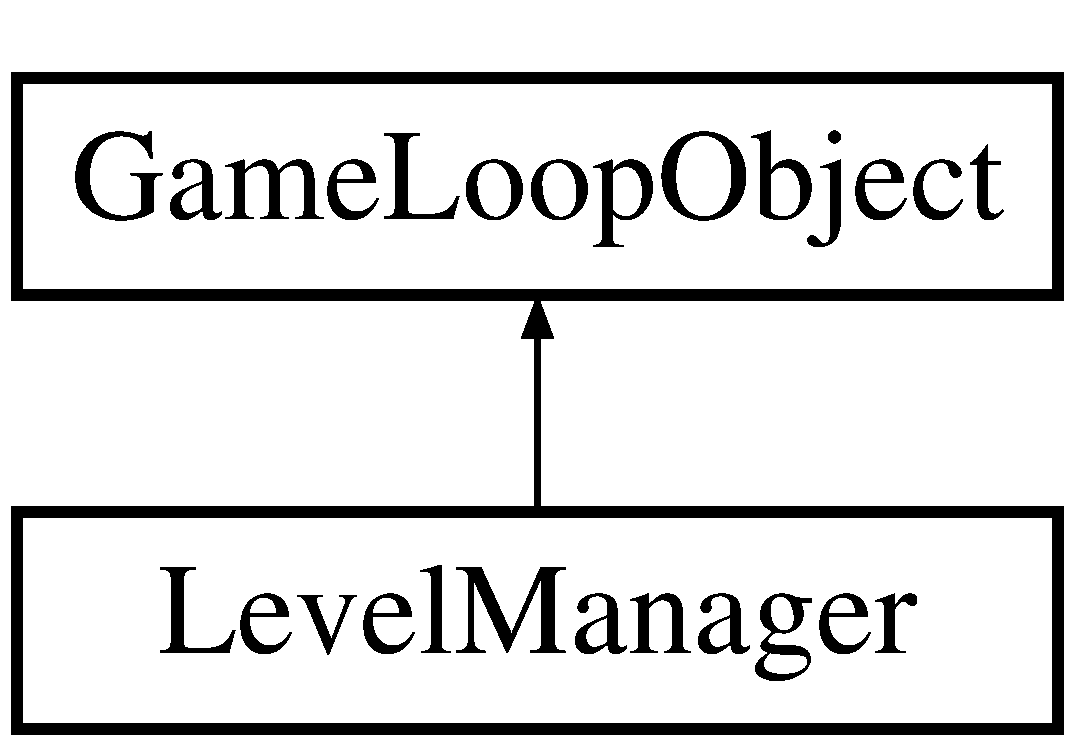
\includegraphics[height=2.000000cm]{class_level_manager}
\end{center}
\end{figure}
\subsection*{Public Member Functions}
\begin{DoxyCompactItemize}
\item 
\hyperlink{class_level_manager_ab420f045161c3663356be1f3d8b1e50d}{Level\+Manager} (\hyperlink{class_player}{Player} \&plr, \hyperlink{class_cursor}{Cursor} \&cr, \hyperlink{struct_controls_input}{Controls\+Input} \&ci)
\begin{DoxyCompactList}\small\item\em The level manager\textquotesingle{}s constructor method. Sets background music. \end{DoxyCompactList}\item 
void \hyperlink{class_level_manager_a7800611361e7c2ae99102e69429456fc}{Update} ()
\begin{DoxyCompactList}\small\item\em Calls the entity controller\textquotesingle{}s update method. \end{DoxyCompactList}\item 
void \hyperlink{class_level_manager_a35cafa518fbbb9fdedfc6a587772bed9}{Draw} (sf\+::\+Render\+Window \&window)
\begin{DoxyCompactList}\small\item\em Calls the entity controller\textquotesingle{}s draw method. \end{DoxyCompactList}\item 
void \hyperlink{class_level_manager_a5e1dd3b7ca877857f1246c7fc95b6a3f}{Reset} ()
\begin{DoxyCompactList}\small\item\em Resets music and player stats. \end{DoxyCompactList}\item 
int \hyperlink{class_level_manager_ae76fd820eb021bb71c2f369074697965}{Get\+Current\+Level} ()
\begin{DoxyCompactList}\small\item\em Returns the current level. \end{DoxyCompactList}\item 
void \hyperlink{class_level_manager_abdd9fde4c4a21da8cb315e9c3a29120a}{Restart\+Current\+Level} ()
\begin{DoxyCompactList}\small\item\em Restarts the current level. \end{DoxyCompactList}\item 
void \hyperlink{class_level_manager_a9c892f8066fa089d7bbc665696bf37c4}{Switch\+To\+Level} (int selected\+Level)
\begin{DoxyCompactList}\small\item\em Switches to a selected level. \end{DoxyCompactList}\item 
int \hyperlink{class_level_manager_aa9423f5861e8eebc14b175da2a2fea91}{Get\+Exiting\+Block} ()
\begin{DoxyCompactList}\small\item\em Asks the entity controller if the player stepped on a level switching block. \end{DoxyCompactList}\item 
\hyperlink{struct_timer}{Timer} \hyperlink{class_level_manager_a8b08bd6bc69bf5877a0e159df5f51af8}{Get\+Shake\+Timer} ()
\begin{DoxyCompactList}\small\item\em Gets the shaketimer from the entity controller. \end{DoxyCompactList}\item 
Vector2f \hyperlink{class_level_manager_a6e8ba28b3df63a8babb0cb3551d5660c}{Get\+Spawn\+Point} ()
\begin{DoxyCompactList}\small\item\em Returns the player\textquotesingle{}s original spawn point as a Vector2f. \end{DoxyCompactList}\end{DoxyCompactItemize}


\subsection{Detailed Description}
Works together with the \hyperlink{class_playing_state}{Playing\+State} to handle maps, entities and music. 

The level manager loads the map of the current level, creates a corresponding entity controller and handles background music. 

Definition at line 19 of file Level\+Manager.\+hpp.



\subsection{Constructor \& Destructor Documentation}
\mbox{\Hypertarget{class_level_manager_ab420f045161c3663356be1f3d8b1e50d}\label{class_level_manager_ab420f045161c3663356be1f3d8b1e50d}} 
\index{Level\+Manager@{Level\+Manager}!Level\+Manager@{Level\+Manager}}
\index{Level\+Manager@{Level\+Manager}!Level\+Manager@{Level\+Manager}}
\subsubsection{\texorpdfstring{Level\+Manager()}{LevelManager()}}
{\footnotesize\ttfamily Level\+Manager\+::\+Level\+Manager (\begin{DoxyParamCaption}\item[{\hyperlink{class_player}{Player} \&}]{plr,  }\item[{\hyperlink{class_cursor}{Cursor} \&}]{cr,  }\item[{\hyperlink{struct_controls_input}{Controls\+Input} \&}]{ci }\end{DoxyParamCaption})}



The level manager\textquotesingle{}s constructor method. Sets background music. 

\textquotesingle{}nuff said. 

Definition at line 6 of file Level\+Manager.\+cpp.



\subsection{Member Function Documentation}
\mbox{\Hypertarget{class_level_manager_a35cafa518fbbb9fdedfc6a587772bed9}\label{class_level_manager_a35cafa518fbbb9fdedfc6a587772bed9}} 
\index{Level\+Manager@{Level\+Manager}!Draw@{Draw}}
\index{Draw@{Draw}!Level\+Manager@{Level\+Manager}}
\subsubsection{\texorpdfstring{Draw()}{Draw()}}
{\footnotesize\ttfamily void Level\+Manager\+::\+Draw (\begin{DoxyParamCaption}\item[{sf\+::\+Render\+Window \&}]{window }\end{DoxyParamCaption})\hspace{0.3cm}{\ttfamily [virtual]}}



Calls the entity controller\textquotesingle{}s draw method. 

\textquotesingle{}nuff said. 

Reimplemented from \hyperlink{class_game_loop_object_a0572a88e5b98fa8a41078260d152202d}{Game\+Loop\+Object}.



Definition at line 22 of file Level\+Manager.\+cpp.

\mbox{\Hypertarget{class_level_manager_ae76fd820eb021bb71c2f369074697965}\label{class_level_manager_ae76fd820eb021bb71c2f369074697965}} 
\index{Level\+Manager@{Level\+Manager}!Get\+Current\+Level@{Get\+Current\+Level}}
\index{Get\+Current\+Level@{Get\+Current\+Level}!Level\+Manager@{Level\+Manager}}
\subsubsection{\texorpdfstring{Get\+Current\+Level()}{GetCurrentLevel()}}
{\footnotesize\ttfamily int Level\+Manager\+::\+Get\+Current\+Level (\begin{DoxyParamCaption}{ }\end{DoxyParamCaption})}



Returns the current level. 

Returns an int with the current level. Nothing else. 

Definition at line 26 of file Level\+Manager.\+cpp.

\mbox{\Hypertarget{class_level_manager_aa9423f5861e8eebc14b175da2a2fea91}\label{class_level_manager_aa9423f5861e8eebc14b175da2a2fea91}} 
\index{Level\+Manager@{Level\+Manager}!Get\+Exiting\+Block@{Get\+Exiting\+Block}}
\index{Get\+Exiting\+Block@{Get\+Exiting\+Block}!Level\+Manager@{Level\+Manager}}
\subsubsection{\texorpdfstring{Get\+Exiting\+Block()}{GetExitingBlock()}}
{\footnotesize\ttfamily int Level\+Manager\+::\+Get\+Exiting\+Block (\begin{DoxyParamCaption}{ }\end{DoxyParamCaption})}



Asks the entity controller if the player stepped on a level switching block. 

Calls a method in the entity controller that checks if the player collides with a level switching block. The value returned tells to which level the game should switch. 

Definition at line 96 of file Level\+Manager.\+cpp.

\mbox{\Hypertarget{class_level_manager_a8b08bd6bc69bf5877a0e159df5f51af8}\label{class_level_manager_a8b08bd6bc69bf5877a0e159df5f51af8}} 
\index{Level\+Manager@{Level\+Manager}!Get\+Shake\+Timer@{Get\+Shake\+Timer}}
\index{Get\+Shake\+Timer@{Get\+Shake\+Timer}!Level\+Manager@{Level\+Manager}}
\subsubsection{\texorpdfstring{Get\+Shake\+Timer()}{GetShakeTimer()}}
{\footnotesize\ttfamily \hyperlink{struct_timer}{Timer} Level\+Manager\+::\+Get\+Shake\+Timer (\begin{DoxyParamCaption}{ }\end{DoxyParamCaption})}



Gets the shaketimer from the entity controller. 

\textquotesingle{}nuff said. 

Definition at line 100 of file Level\+Manager.\+cpp.

\mbox{\Hypertarget{class_level_manager_a6e8ba28b3df63a8babb0cb3551d5660c}\label{class_level_manager_a6e8ba28b3df63a8babb0cb3551d5660c}} 
\index{Level\+Manager@{Level\+Manager}!Get\+Spawn\+Point@{Get\+Spawn\+Point}}
\index{Get\+Spawn\+Point@{Get\+Spawn\+Point}!Level\+Manager@{Level\+Manager}}
\subsubsection{\texorpdfstring{Get\+Spawn\+Point()}{GetSpawnPoint()}}
{\footnotesize\ttfamily Vector2f Level\+Manager\+::\+Get\+Spawn\+Point (\begin{DoxyParamCaption}{ }\end{DoxyParamCaption})}



Returns the player\textquotesingle{}s original spawn point as a Vector2f. 

\textquotesingle{}nuff said. 

Definition at line 104 of file Level\+Manager.\+cpp.

\mbox{\Hypertarget{class_level_manager_a5e1dd3b7ca877857f1246c7fc95b6a3f}\label{class_level_manager_a5e1dd3b7ca877857f1246c7fc95b6a3f}} 
\index{Level\+Manager@{Level\+Manager}!Reset@{Reset}}
\index{Reset@{Reset}!Level\+Manager@{Level\+Manager}}
\subsubsection{\texorpdfstring{Reset()}{Reset()}}
{\footnotesize\ttfamily void Level\+Manager\+::\+Reset (\begin{DoxyParamCaption}{ }\end{DoxyParamCaption})\hspace{0.3cm}{\ttfamily [virtual]}}



Resets music and player stats. 

\textquotesingle{}nuff said. 

Reimplemented from \hyperlink{class_game_loop_object_af61e973be170cb9437a5b7d9ecd6ef53}{Game\+Loop\+Object}.



Definition at line 88 of file Level\+Manager.\+cpp.

\mbox{\Hypertarget{class_level_manager_abdd9fde4c4a21da8cb315e9c3a29120a}\label{class_level_manager_abdd9fde4c4a21da8cb315e9c3a29120a}} 
\index{Level\+Manager@{Level\+Manager}!Restart\+Current\+Level@{Restart\+Current\+Level}}
\index{Restart\+Current\+Level@{Restart\+Current\+Level}!Level\+Manager@{Level\+Manager}}
\subsubsection{\texorpdfstring{Restart\+Current\+Level()}{RestartCurrentLevel()}}
{\footnotesize\ttfamily void Level\+Manager\+::\+Restart\+Current\+Level (\begin{DoxyParamCaption}{ }\end{DoxyParamCaption})}



Restarts the current level. 

Restarts the current level by resetting player stats, resurrecting the player, reloading the map and reloading the entity controller. 

Definition at line 30 of file Level\+Manager.\+cpp.

\mbox{\Hypertarget{class_level_manager_a9c892f8066fa089d7bbc665696bf37c4}\label{class_level_manager_a9c892f8066fa089d7bbc665696bf37c4}} 
\index{Level\+Manager@{Level\+Manager}!Switch\+To\+Level@{Switch\+To\+Level}}
\index{Switch\+To\+Level@{Switch\+To\+Level}!Level\+Manager@{Level\+Manager}}
\subsubsection{\texorpdfstring{Switch\+To\+Level()}{SwitchToLevel()}}
{\footnotesize\ttfamily void Level\+Manager\+::\+Switch\+To\+Level (\begin{DoxyParamCaption}\item[{int}]{selected\+Level }\end{DoxyParamCaption})}



Switches to a selected level. 

Loads a new map and entity controller for the new level. Does not reset player stats etc. 

Definition at line 57 of file Level\+Manager.\+cpp.

\mbox{\Hypertarget{class_level_manager_a7800611361e7c2ae99102e69429456fc}\label{class_level_manager_a7800611361e7c2ae99102e69429456fc}} 
\index{Level\+Manager@{Level\+Manager}!Update@{Update}}
\index{Update@{Update}!Level\+Manager@{Level\+Manager}}
\subsubsection{\texorpdfstring{Update()}{Update()}}
{\footnotesize\ttfamily void Level\+Manager\+::\+Update (\begin{DoxyParamCaption}{ }\end{DoxyParamCaption})\hspace{0.3cm}{\ttfamily [virtual]}}



Calls the entity controller\textquotesingle{}s update method. 

\textquotesingle{}nuff said. 

Reimplemented from \hyperlink{class_game_loop_object_ae36a15981f1dd3f3bea6050473490349}{Game\+Loop\+Object}.



Definition at line 18 of file Level\+Manager.\+cpp.



The documentation for this class was generated from the following files\+:\begin{DoxyCompactItemize}
\item 
C\+:/\+Users/joost/\+Documents/\+Git\+Hub/topdown/\+Code/\+Team\+Topdown/\+Team\+Topdown/\hyperlink{_level_manager_8hpp}{Level\+Manager.\+hpp}\item 
C\+:/\+Users/joost/\+Documents/\+Git\+Hub/topdown/\+Code/\+Team\+Topdown/\+Team\+Topdown/\hyperlink{_level_manager_8cpp}{Level\+Manager.\+cpp}\end{DoxyCompactItemize}

\hypertarget{class_main_menu_state}{}\section{Main\+Menu\+State Class Reference}
\label{class_main_menu_state}\index{Main\+Menu\+State@{Main\+Menu\+State}}


The gamestate that is the game\textquotesingle{}s main menu.  




{\ttfamily \#include $<$Main\+Menu\+State.\+hpp$>$}

Inheritance diagram for Main\+Menu\+State\+:\begin{figure}[H]
\begin{center}
\leavevmode
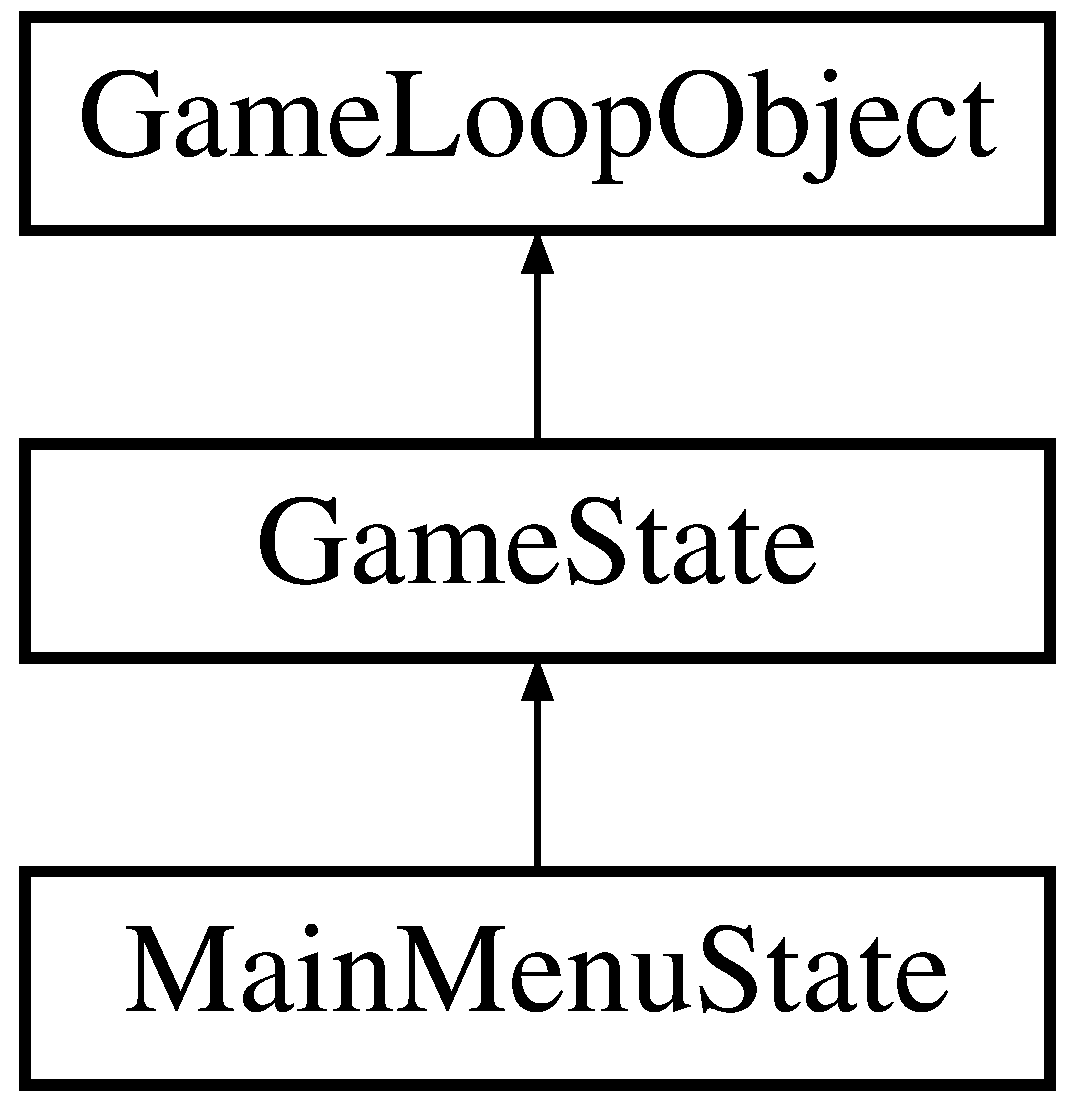
\includegraphics[height=3.000000cm]{class_main_menu_state}
\end{center}
\end{figure}
\subsection*{Public Member Functions}
\begin{DoxyCompactItemize}
\item 
\hyperlink{class_main_menu_state_a319907358bf3fbbc42cab50ac5fdebdc}{Main\+Menu\+State} (sf\+::\+Render\+Window \&window, \hyperlink{class_game_state_manager}{Game\+State\+Manager} \&gsm, \hyperlink{struct_controls_input}{Controls\+Input} \&ci, \hyperlink{class_level_manager}{Level\+Manager} \&lm, \hyperlink{class_camera}{Camera} \&cm, \hyperlink{class_cursor}{Cursor} \&cr, \hyperlink{class_player}{Player} \&plr)
\begin{DoxyCompactList}\small\item\em The main menu\textquotesingle{}s constructor method. \end{DoxyCompactList}\item 
void \hyperlink{class_main_menu_state_ac332ae234d282f4e6657ee9d0685b7ff}{Handle\+Input} ()
\begin{DoxyCompactList}\small\item\em The main menu\textquotesingle{}s game loop method for handling keyboard and mouse input. \end{DoxyCompactList}\item 
void \hyperlink{class_main_menu_state_a35ec35095919057ef7373906b09a9d30}{Update} ()
\begin{DoxyCompactList}\small\item\em The main menu\textquotesingle{}s game loop method for updating the game. \end{DoxyCompactList}\item 
void \hyperlink{class_main_menu_state_a6965e10d73953ef09c63a64685136307}{Draw} (sf\+::\+Render\+Window \&window)
\begin{DoxyCompactList}\small\item\em The main menu\textquotesingle{}s game loop method for drawing on the window. \end{DoxyCompactList}\item 
void \hyperlink{class_main_menu_state_a6f6c9814913db12bc9578411620f9b56}{Reset} ()
\begin{DoxyCompactList}\small\item\em The state\textquotesingle{}s reset method. Resets the menu to default. \end{DoxyCompactList}\item 
void \hyperlink{class_main_menu_state_a632b2e5cc71503e46a59fd29501f6869}{transition\+From\+This} ()
\end{DoxyCompactItemize}


\subsection{Detailed Description}
The gamestate that is the game\textquotesingle{}s main menu. 

In this gamestate, the player can start a new game, enter the level select menu to choose which level to play, see the high scores (not implemented), the credits and exit the game. 

Definition at line 24 of file Main\+Menu\+State.\+hpp.



\subsection{Constructor \& Destructor Documentation}
\mbox{\Hypertarget{class_main_menu_state_a319907358bf3fbbc42cab50ac5fdebdc}\label{class_main_menu_state_a319907358bf3fbbc42cab50ac5fdebdc}} 
\index{Main\+Menu\+State@{Main\+Menu\+State}!Main\+Menu\+State@{Main\+Menu\+State}}
\index{Main\+Menu\+State@{Main\+Menu\+State}!Main\+Menu\+State@{Main\+Menu\+State}}
\subsubsection{\texorpdfstring{Main\+Menu\+State()}{MainMenuState()}}
{\footnotesize\ttfamily Main\+Menu\+State\+::\+Main\+Menu\+State (\begin{DoxyParamCaption}\item[{sf\+::\+Render\+Window \&}]{window,  }\item[{\hyperlink{class_game_state_manager}{Game\+State\+Manager} \&}]{gsm,  }\item[{\hyperlink{struct_controls_input}{Controls\+Input} \&}]{ci,  }\item[{\hyperlink{class_level_manager}{Level\+Manager} \&}]{lm,  }\item[{\hyperlink{class_camera}{Camera} \&}]{cm,  }\item[{\hyperlink{class_cursor}{Cursor} \&}]{cr,  }\item[{\hyperlink{class_player}{Player} \&}]{plr }\end{DoxyParamCaption})}



The main menu\textquotesingle{}s constructor method. 

The main menu\textquotesingle{}s constructor requires a window to draw on, the gamestatemanger to switch to other gamestates, controlsinput to read keyboard and mouse input, the levelmanager to set the level to play, the cursor (not used anymore) and the player to access the H\+UD to reset time. 

Definition at line 6 of file Main\+Menu\+State.\+cpp.



\subsection{Member Function Documentation}
\mbox{\Hypertarget{class_main_menu_state_a6965e10d73953ef09c63a64685136307}\label{class_main_menu_state_a6965e10d73953ef09c63a64685136307}} 
\index{Main\+Menu\+State@{Main\+Menu\+State}!Draw@{Draw}}
\index{Draw@{Draw}!Main\+Menu\+State@{Main\+Menu\+State}}
\subsubsection{\texorpdfstring{Draw()}{Draw()}}
{\footnotesize\ttfamily void Main\+Menu\+State\+::\+Draw (\begin{DoxyParamCaption}\item[{sf\+::\+Render\+Window \&}]{window }\end{DoxyParamCaption})\hspace{0.3cm}{\ttfamily [virtual]}}



The main menu\textquotesingle{}s game loop method for drawing on the window. 

Draws the background and either the main menu or the level select menu. 

Reimplemented from \hyperlink{class_game_state_a8741c5c696c6c366beb4b845c08c3cf8}{Game\+State}.



Definition at line 157 of file Main\+Menu\+State.\+cpp.

\mbox{\Hypertarget{class_main_menu_state_ac332ae234d282f4e6657ee9d0685b7ff}\label{class_main_menu_state_ac332ae234d282f4e6657ee9d0685b7ff}} 
\index{Main\+Menu\+State@{Main\+Menu\+State}!Handle\+Input@{Handle\+Input}}
\index{Handle\+Input@{Handle\+Input}!Main\+Menu\+State@{Main\+Menu\+State}}
\subsubsection{\texorpdfstring{Handle\+Input()}{HandleInput()}}
{\footnotesize\ttfamily void Main\+Menu\+State\+::\+Handle\+Input (\begin{DoxyParamCaption}{ }\end{DoxyParamCaption})\hspace{0.3cm}{\ttfamily [virtual]}}



The main menu\textquotesingle{}s game loop method for handling keyboard and mouse input. 

Handles input for the main menu. 

Reimplemented from \hyperlink{class_game_state_a8bce2828cee99ae7c07322804531fd01}{Game\+State}.



Definition at line 55 of file Main\+Menu\+State.\+cpp.

\mbox{\Hypertarget{class_main_menu_state_a6f6c9814913db12bc9578411620f9b56}\label{class_main_menu_state_a6f6c9814913db12bc9578411620f9b56}} 
\index{Main\+Menu\+State@{Main\+Menu\+State}!Reset@{Reset}}
\index{Reset@{Reset}!Main\+Menu\+State@{Main\+Menu\+State}}
\subsubsection{\texorpdfstring{Reset()}{Reset()}}
{\footnotesize\ttfamily void Main\+Menu\+State\+::\+Reset (\begin{DoxyParamCaption}{ }\end{DoxyParamCaption})\hspace{0.3cm}{\ttfamily [virtual]}}



The state\textquotesingle{}s reset method. Resets the menu to default. 

Resets main menu if level select menu is up. Stops music. 

Reimplemented from \hyperlink{class_game_state_a46ac6317883dff0eba4f8f305af6b6bb}{Game\+State}.



Definition at line 169 of file Main\+Menu\+State.\+cpp.

\mbox{\Hypertarget{class_main_menu_state_a632b2e5cc71503e46a59fd29501f6869}\label{class_main_menu_state_a632b2e5cc71503e46a59fd29501f6869}} 
\index{Main\+Menu\+State@{Main\+Menu\+State}!transition\+From\+This@{transition\+From\+This}}
\index{transition\+From\+This@{transition\+From\+This}!Main\+Menu\+State@{Main\+Menu\+State}}
\subsubsection{\texorpdfstring{transition\+From\+This()}{transitionFromThis()}}
{\footnotesize\ttfamily void Main\+Menu\+State\+::transition\+From\+This (\begin{DoxyParamCaption}{ }\end{DoxyParamCaption})}

void transition\+From\+This /brief Initiates a screen transition towards the next state. 

Definition at line 177 of file Main\+Menu\+State.\+cpp.

\mbox{\Hypertarget{class_main_menu_state_a35ec35095919057ef7373906b09a9d30}\label{class_main_menu_state_a35ec35095919057ef7373906b09a9d30}} 
\index{Main\+Menu\+State@{Main\+Menu\+State}!Update@{Update}}
\index{Update@{Update}!Main\+Menu\+State@{Main\+Menu\+State}}
\subsubsection{\texorpdfstring{Update()}{Update()}}
{\footnotesize\ttfamily void Main\+Menu\+State\+::\+Update (\begin{DoxyParamCaption}{ }\end{DoxyParamCaption})\hspace{0.3cm}{\ttfamily [virtual]}}



The main menu\textquotesingle{}s game loop method for updating the game. 

Starts main menu music. Updates the main menu. 

Reimplemented from \hyperlink{class_game_state_a5be51b634f95bc6e57066ad6931aa18b}{Game\+State}.



Definition at line 142 of file Main\+Menu\+State.\+cpp.



The documentation for this class was generated from the following files\+:\begin{DoxyCompactItemize}
\item 
C\+:/\+Users/joost/\+Documents/\+Git\+Hub/topdown/\+Code/\+Team\+Topdown/\+Team\+Topdown/\hyperlink{_main_menu_state_8hpp}{Main\+Menu\+State.\+hpp}\item 
C\+:/\+Users/joost/\+Documents/\+Git\+Hub/topdown/\+Code/\+Team\+Topdown/\+Team\+Topdown/\hyperlink{_main_menu_state_8cpp}{Main\+Menu\+State.\+cpp}\end{DoxyCompactItemize}

\hypertarget{class_map}{}\section{Map Class Reference}
\label{class_map}\index{Map@{Map}}


Creates an entity list based on a collision map This class creates a list of entities based on the red value of a .png-\/file. We loop through the pixels to determine a position. The tile size is constant and set. Once we find a pixel with a red-\/value of 0, we make it our spawnpoint. If it\textquotesingle{}s a 1, we spawn a wall at that position with the standard tilesize and add it to the entity list. A red-\/value of 2 indicates an enemy waypoint. This will either create a new enemy from that waypoint, or add the waypoint to an already existing enemy. In creating such a waypoint, the green-\/value of the pixel determines the enemy by ID and the blue-\/value determines the order of waypoints. In that way, we only have to loop through the pixel map once. A red-\/value of 3 is a crate, and a red-\/value of 4 is a set of spikes. In this case, the green value represents the starting state (down, rising or up). Finally a red-\/value of 5 represents an exit, with its green-\/value being the level number (1-\/based!)  




{\ttfamily \#include $<$Map.\+h$>$}

\subsection*{Public Member Functions}
\begin{DoxyCompactItemize}
\item 
\hyperlink{class_map_a1b9128df3f2c9aa5ff56130a3530e8a1}{Map} (String background\+File, String shadow\+Map\+File, String collision\+Map\+File, \hyperlink{class_player}{Player} \&our\+Player)
\item 
\hyperlink{class_map_aa403fbe09394ccf39747588f5168e3b2}{$\sim$\+Map} ()
\item 
std\+::vector$<$ \hyperlink{class_entity}{Entity} $\ast$ $>$ \hyperlink{class_map_a2321c241804c5ed69c0bc7d073f901fd}{get\+Entities} ()
\item 
std\+::vector$<$ \hyperlink{class_enemy}{Enemy} $\ast$ $>$ \hyperlink{class_map_a8796db77b21d899391c8163f3accf32c}{get\+Enemies} ()
\item 
std\+::vector$<$ \hyperlink{class_exit}{Exit} $\ast$ $>$ \hyperlink{class_map_a1c3f034c6072fe1103626cd9f5685094}{get\+Exits} ()
\item 
std\+::vector$<$ \hyperlink{class_turret}{Turret} $\ast$ $>$ \hyperlink{class_map_ab8f9839fd7d6e6838772cbad9cc9dc34}{get\+Turrets} ()
\item 
Vector2f \hyperlink{class_map_a15095789dcc043bbed23092f37447731}{get\+Spawn\+Point} ()
\end{DoxyCompactItemize}
\subsection*{Public Attributes}
\begin{DoxyCompactItemize}
\item 
\hyperlink{class_graphic}{Graphic} \hyperlink{class_map_ae0b54e9c9926c2b9a369e351a8f6e7b7}{background}
\item 
\hyperlink{class_graphic}{Graphic} \hyperlink{class_map_a444d10c1cf7a759976a72dcec8908e62}{shadow\+Map}
\end{DoxyCompactItemize}


\subsection{Detailed Description}
Creates an entity list based on a collision map This class creates a list of entities based on the red value of a .png-\/file. We loop through the pixels to determine a position. The tile size is constant and set. Once we find a pixel with a red-\/value of 0, we make it our spawnpoint. If it\textquotesingle{}s a 1, we spawn a wall at that position with the standard tilesize and add it to the entity list. A red-\/value of 2 indicates an enemy waypoint. This will either create a new enemy from that waypoint, or add the waypoint to an already existing enemy. In creating such a waypoint, the green-\/value of the pixel determines the enemy by ID and the blue-\/value determines the order of waypoints. In that way, we only have to loop through the pixel map once. A red-\/value of 3 is a crate, and a red-\/value of 4 is a set of spikes. In this case, the green value represents the starting state (down, rising or up). Finally a red-\/value of 5 represents an exit, with its green-\/value being the level number (1-\/based!) 

Definition at line 29 of file Map.\+h.



\subsection{Constructor \& Destructor Documentation}
\mbox{\Hypertarget{class_map_a1b9128df3f2c9aa5ff56130a3530e8a1}\label{class_map_a1b9128df3f2c9aa5ff56130a3530e8a1}} 
\index{Map@{Map}!Map@{Map}}
\index{Map@{Map}!Map@{Map}}
\subsubsection{\texorpdfstring{Map()}{Map()}}
{\footnotesize\ttfamily Map\+::\+Map (\begin{DoxyParamCaption}\item[{String}]{background\+File,  }\item[{String}]{shadow\+Map\+File,  }\item[{String}]{collision\+Map\+File,  }\item[{\hyperlink{class_player}{Player} \&}]{our\+Player }\end{DoxyParamCaption})}



Definition at line 4 of file Map.\+cpp.

\mbox{\Hypertarget{class_map_aa403fbe09394ccf39747588f5168e3b2}\label{class_map_aa403fbe09394ccf39747588f5168e3b2}} 
\index{Map@{Map}!````~Map@{$\sim$\+Map}}
\index{````~Map@{$\sim$\+Map}!Map@{Map}}
\subsubsection{\texorpdfstring{$\sim$\+Map()}{~Map()}}
{\footnotesize\ttfamily Map\+::$\sim$\+Map (\begin{DoxyParamCaption}{ }\end{DoxyParamCaption})}



Definition at line 51 of file Map.\+cpp.



\subsection{Member Function Documentation}
\mbox{\Hypertarget{class_map_a8796db77b21d899391c8163f3accf32c}\label{class_map_a8796db77b21d899391c8163f3accf32c}} 
\index{Map@{Map}!get\+Enemies@{get\+Enemies}}
\index{get\+Enemies@{get\+Enemies}!Map@{Map}}
\subsubsection{\texorpdfstring{get\+Enemies()}{getEnemies()}}
{\footnotesize\ttfamily std\+::vector$<$ \hyperlink{class_enemy}{Enemy} $\ast$ $>$ Map\+::get\+Enemies (\begin{DoxyParamCaption}{ }\end{DoxyParamCaption})}



Definition at line 89 of file Map.\+cpp.

\mbox{\Hypertarget{class_map_a2321c241804c5ed69c0bc7d073f901fd}\label{class_map_a2321c241804c5ed69c0bc7d073f901fd}} 
\index{Map@{Map}!get\+Entities@{get\+Entities}}
\index{get\+Entities@{get\+Entities}!Map@{Map}}
\subsubsection{\texorpdfstring{get\+Entities()}{getEntities()}}
{\footnotesize\ttfamily std\+::vector$<$ \hyperlink{class_entity}{Entity} $\ast$ $>$ Map\+::get\+Entities (\begin{DoxyParamCaption}{ }\end{DoxyParamCaption})}



Definition at line 85 of file Map.\+cpp.

\mbox{\Hypertarget{class_map_a1c3f034c6072fe1103626cd9f5685094}\label{class_map_a1c3f034c6072fe1103626cd9f5685094}} 
\index{Map@{Map}!get\+Exits@{get\+Exits}}
\index{get\+Exits@{get\+Exits}!Map@{Map}}
\subsubsection{\texorpdfstring{get\+Exits()}{getExits()}}
{\footnotesize\ttfamily std\+::vector$<$ \hyperlink{class_exit}{Exit} $\ast$ $>$ Map\+::get\+Exits (\begin{DoxyParamCaption}{ }\end{DoxyParamCaption})}



Definition at line 93 of file Map.\+cpp.

\mbox{\Hypertarget{class_map_a15095789dcc043bbed23092f37447731}\label{class_map_a15095789dcc043bbed23092f37447731}} 
\index{Map@{Map}!get\+Spawn\+Point@{get\+Spawn\+Point}}
\index{get\+Spawn\+Point@{get\+Spawn\+Point}!Map@{Map}}
\subsubsection{\texorpdfstring{get\+Spawn\+Point()}{getSpawnPoint()}}
{\footnotesize\ttfamily Vector2f Map\+::get\+Spawn\+Point (\begin{DoxyParamCaption}{ }\end{DoxyParamCaption})}



Definition at line 100 of file Map.\+cpp.

\mbox{\Hypertarget{class_map_ab8f9839fd7d6e6838772cbad9cc9dc34}\label{class_map_ab8f9839fd7d6e6838772cbad9cc9dc34}} 
\index{Map@{Map}!get\+Turrets@{get\+Turrets}}
\index{get\+Turrets@{get\+Turrets}!Map@{Map}}
\subsubsection{\texorpdfstring{get\+Turrets()}{getTurrets()}}
{\footnotesize\ttfamily std\+::vector$<$ \hyperlink{class_turret}{Turret} $\ast$ $>$ Map\+::get\+Turrets (\begin{DoxyParamCaption}{ }\end{DoxyParamCaption})}



Definition at line 97 of file Map.\+cpp.



\subsection{Member Data Documentation}
\mbox{\Hypertarget{class_map_ae0b54e9c9926c2b9a369e351a8f6e7b7}\label{class_map_ae0b54e9c9926c2b9a369e351a8f6e7b7}} 
\index{Map@{Map}!background@{background}}
\index{background@{background}!Map@{Map}}
\subsubsection{\texorpdfstring{background}{background}}
{\footnotesize\ttfamily \hyperlink{class_graphic}{Graphic} Map\+::background}



Definition at line 46 of file Map.\+h.

\mbox{\Hypertarget{class_map_a444d10c1cf7a759976a72dcec8908e62}\label{class_map_a444d10c1cf7a759976a72dcec8908e62}} 
\index{Map@{Map}!shadow\+Map@{shadow\+Map}}
\index{shadow\+Map@{shadow\+Map}!Map@{Map}}
\subsubsection{\texorpdfstring{shadow\+Map}{shadowMap}}
{\footnotesize\ttfamily \hyperlink{class_graphic}{Graphic} Map\+::shadow\+Map}



Definition at line 47 of file Map.\+h.



The documentation for this class was generated from the following files\+:\begin{DoxyCompactItemize}
\item 
C\+:/\+Users/joost/\+Documents/\+Git\+Hub/topdown/\+Code/\+Team\+Topdown/\+Team\+Topdown/\hyperlink{_map_8h}{Map.\+h}\item 
C\+:/\+Users/joost/\+Documents/\+Git\+Hub/topdown/\+Code/\+Team\+Topdown/\+Team\+Topdown/\hyperlink{_map_8cpp}{Map.\+cpp}\end{DoxyCompactItemize}

\hypertarget{class_menu}{}\section{Menu Class Reference}
\label{class_menu}\index{Menu@{Menu}}


A auto-\/resizing menu of Clickable\+Buttons.  




{\ttfamily \#include $<$Menu.\+hpp$>$}

Inheritance diagram for Menu\+:\begin{figure}[H]
\begin{center}
\leavevmode
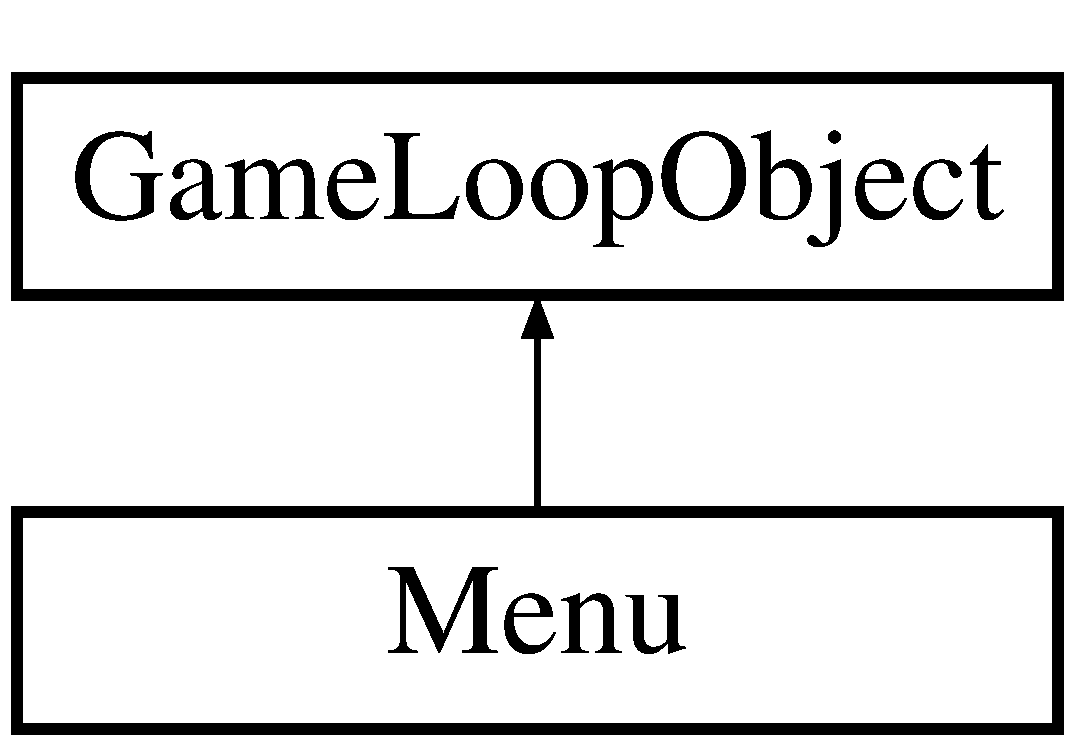
\includegraphics[height=2.000000cm]{class_menu}
\end{center}
\end{figure}
\subsection*{Public Member Functions}
\begin{DoxyCompactItemize}
\item 
\hyperlink{class_menu_accc796ef85a8a1834ebf5cd04db2334c}{Menu} (sf\+::\+Render\+Window \&window, sf\+::\+Vector2f position, sf\+::\+Vector2f button\+Size, std\+::vector$<$ std\+::string $>$ button\+Names, \hyperlink{class_camera}{Camera} \&camera, bool is\+Visible=1, bool auto\+Calc\+Width=0, int offset=0, bool update\+To\+Center=0)
\begin{DoxyCompactList}\small\item\em Constructor. \end{DoxyCompactList}\item 
void \hyperlink{class_menu_a0cb3596524ed7fd021f999860b563bf8}{Handle\+Input} ()
\begin{DoxyCompactList}\small\item\em The menu\textquotesingle{}s user input handling method. \end{DoxyCompactList}\item 
void \hyperlink{class_menu_af29d71473a414e31e914bc637840cb3e}{Update} ()
\begin{DoxyCompactList}\small\item\em The menu\textquotesingle{}s update method. \end{DoxyCompactList}\item 
void \hyperlink{class_menu_a9052b7f20dcf6d9ed47d87f16fcfe5e9}{Draw} (sf\+::\+Render\+Window \&window)
\begin{DoxyCompactList}\small\item\em The menu\textquotesingle{}s draw method. \end{DoxyCompactList}\item 
void \hyperlink{class_menu_af48862906748cee615d455eae4ee3349}{Reset} ()
\begin{DoxyCompactList}\small\item\em The menu\textquotesingle{}s reset method. \end{DoxyCompactList}\item 
void \hyperlink{class_menu_a03141d21380b6c72be54edd7aae33ff4}{Show} ()
\begin{DoxyCompactList}\small\item\em Toggles visibility of the menu to visible. \end{DoxyCompactList}\item 
void \hyperlink{class_menu_a5e035344163bc1d000a4e519181b2688}{Hide} ()
\begin{DoxyCompactList}\small\item\em Toggles visibility of the menu to hidden. \end{DoxyCompactList}\item 
int \hyperlink{class_menu_a2b51455862ea3993a6dbd51ea5fe9f4d}{Get\+Amount\+Of\+Buttons} ()
\begin{DoxyCompactList}\small\item\em Returns an int with the amount of buttons the instance of a menu has. \end{DoxyCompactList}\item 
int \hyperlink{class_menu_a967d011a2868591943e2706750261878}{Get\+Button\+Width} ()
\begin{DoxyCompactList}\small\item\em Returns the width of the buttons in the menu as an int. \end{DoxyCompactList}\item 
int \hyperlink{class_menu_ac75194d487ea0f1eada384f887c78051}{Find\+Button\+Press} ()
\begin{DoxyCompactList}\small\item\em Checks all buttons for a button press and returns which one was pressed. \end{DoxyCompactList}\item 
bool \hyperlink{class_menu_a960228ac37c0f68984e3eac976f63d61}{Is\+Visible} ()
\begin{DoxyCompactList}\small\item\em Checks if the menu is currently visible and returns true or false. \end{DoxyCompactList}\item 
void \hyperlink{class_menu_aa1c57bdd5d83521af8214ac43a68d878}{Reposition\+To\+Center} ()
\begin{DoxyCompactList}\small\item\em Repositions the menu to the center of the window. \end{DoxyCompactList}\end{DoxyCompactItemize}


\subsection{Detailed Description}
A auto-\/resizing menu of Clickable\+Buttons. 

A menu of clickable buttons. The amount of buttons and their texts are chosen on creation. Visibility can be toggled, its size can be auto-\/calculated based on the size of the longest button text, an offset between buttons can be selected and the menu can be auto-\/centered to the center of the screen. 

Definition at line 16 of file Menu.\+hpp.



\subsection{Constructor \& Destructor Documentation}
\mbox{\Hypertarget{class_menu_accc796ef85a8a1834ebf5cd04db2334c}\label{class_menu_accc796ef85a8a1834ebf5cd04db2334c}} 
\index{Menu@{Menu}!Menu@{Menu}}
\index{Menu@{Menu}!Menu@{Menu}}
\subsubsection{\texorpdfstring{Menu()}{Menu()}}
{\footnotesize\ttfamily Menu\+::\+Menu (\begin{DoxyParamCaption}\item[{sf\+::\+Render\+Window \&}]{window,  }\item[{sf\+::\+Vector2f}]{position,  }\item[{sf\+::\+Vector2f}]{button\+Size,  }\item[{std\+::vector$<$ std\+::string $>$}]{button\+Names,  }\item[{\hyperlink{class_camera}{Camera} \&}]{camera,  }\item[{bool}]{is\+Visible = {\ttfamily 1},  }\item[{bool}]{auto\+Calc\+Width = {\ttfamily 0},  }\item[{int}]{offset = {\ttfamily 0},  }\item[{bool}]{update\+To\+Center = {\ttfamily 0} }\end{DoxyParamCaption})}



Constructor. 

To create a menu, you first have to create a std\+::vector of std\+::strings in which you store all your button names (aka the text displayed on the buttons). Then, call the menu\textquotesingle{}s constructor, in which you pass the window, a position (x value of desired origin, y value of menu top) the desired size of the buttons, the list of button names and the camera. Optionally, you can set if the menu is visible or hidden (visible (true) by default), if the button size should be auto-\/calculated (takes the longest button text and resizes all buttons to match the width) if there should be a vertical offset between each button (0 by default) and if the menu\textquotesingle{}s position should be updated to the center of the screen (which is used by the game\textquotesingle{}s pause menu). 

Definition at line 5 of file Menu.\+cpp.



\subsection{Member Function Documentation}
\mbox{\Hypertarget{class_menu_a9052b7f20dcf6d9ed47d87f16fcfe5e9}\label{class_menu_a9052b7f20dcf6d9ed47d87f16fcfe5e9}} 
\index{Menu@{Menu}!Draw@{Draw}}
\index{Draw@{Draw}!Menu@{Menu}}
\subsubsection{\texorpdfstring{Draw()}{Draw()}}
{\footnotesize\ttfamily void Menu\+::\+Draw (\begin{DoxyParamCaption}\item[{sf\+::\+Render\+Window \&}]{window }\end{DoxyParamCaption})\hspace{0.3cm}{\ttfamily [virtual]}}



The menu\textquotesingle{}s draw method. 

Runs the draw methods of all buttons if the menu is set to visible. Else this does nothing. 

Reimplemented from \hyperlink{class_game_loop_object_a0572a88e5b98fa8a41078260d152202d}{Game\+Loop\+Object}.



Definition at line 52 of file Menu.\+cpp.

\mbox{\Hypertarget{class_menu_ac75194d487ea0f1eada384f887c78051}\label{class_menu_ac75194d487ea0f1eada384f887c78051}} 
\index{Menu@{Menu}!Find\+Button\+Press@{Find\+Button\+Press}}
\index{Find\+Button\+Press@{Find\+Button\+Press}!Menu@{Menu}}
\subsubsection{\texorpdfstring{Find\+Button\+Press()}{FindButtonPress()}}
{\footnotesize\ttfamily int Menu\+::\+Find\+Button\+Press (\begin{DoxyParamCaption}{ }\end{DoxyParamCaption})}



Checks all buttons for a button press and returns which one was pressed. 

Runs the Is\+Pressed method of all buttons and returns an int with the number of the button that was pressed. Counts from 1 to end. If 0 is returned, no button was pressed. 

Definition at line 87 of file Menu.\+cpp.

\mbox{\Hypertarget{class_menu_a2b51455862ea3993a6dbd51ea5fe9f4d}\label{class_menu_a2b51455862ea3993a6dbd51ea5fe9f4d}} 
\index{Menu@{Menu}!Get\+Amount\+Of\+Buttons@{Get\+Amount\+Of\+Buttons}}
\index{Get\+Amount\+Of\+Buttons@{Get\+Amount\+Of\+Buttons}!Menu@{Menu}}
\subsubsection{\texorpdfstring{Get\+Amount\+Of\+Buttons()}{GetAmountOfButtons()}}
{\footnotesize\ttfamily int Menu\+::\+Get\+Amount\+Of\+Buttons (\begin{DoxyParamCaption}{ }\end{DoxyParamCaption})}



Returns an int with the amount of buttons the instance of a menu has. 

Returns the amount\+Of\+Buttons it. Does nothing else. 

Definition at line 78 of file Menu.\+cpp.

\mbox{\Hypertarget{class_menu_a967d011a2868591943e2706750261878}\label{class_menu_a967d011a2868591943e2706750261878}} 
\index{Menu@{Menu}!Get\+Button\+Width@{Get\+Button\+Width}}
\index{Get\+Button\+Width@{Get\+Button\+Width}!Menu@{Menu}}
\subsubsection{\texorpdfstring{Get\+Button\+Width()}{GetButtonWidth()}}
{\footnotesize\ttfamily int Menu\+::\+Get\+Button\+Width (\begin{DoxyParamCaption}{ }\end{DoxyParamCaption})}



Returns the width of the buttons in the menu as an int. 

\textquotesingle{}nuff said. 

Definition at line 83 of file Menu.\+cpp.

\mbox{\Hypertarget{class_menu_a0cb3596524ed7fd021f999860b563bf8}\label{class_menu_a0cb3596524ed7fd021f999860b563bf8}} 
\index{Menu@{Menu}!Handle\+Input@{Handle\+Input}}
\index{Handle\+Input@{Handle\+Input}!Menu@{Menu}}
\subsubsection{\texorpdfstring{Handle\+Input()}{HandleInput()}}
{\footnotesize\ttfamily void Menu\+::\+Handle\+Input (\begin{DoxyParamCaption}{ }\end{DoxyParamCaption})\hspace{0.3cm}{\ttfamily [virtual]}}



The menu\textquotesingle{}s user input handling method. 

Runs the Handle\+Input methods of all buttons in the menu if the menu is visible. Else this does nothing. 

Reimplemented from \hyperlink{class_game_loop_object_aecab111d504b7f4590045ca7c83a36de}{Game\+Loop\+Object}.



Definition at line 31 of file Menu.\+cpp.

\mbox{\Hypertarget{class_menu_a5e035344163bc1d000a4e519181b2688}\label{class_menu_a5e035344163bc1d000a4e519181b2688}} 
\index{Menu@{Menu}!Hide@{Hide}}
\index{Hide@{Hide}!Menu@{Menu}}
\subsubsection{\texorpdfstring{Hide()}{Hide()}}
{\footnotesize\ttfamily void Menu\+::\+Hide (\begin{DoxyParamCaption}{ }\end{DoxyParamCaption})}



Toggles visibility of the menu to hidden. 

Sets the bool is\+Visible to -\/1. Does nothing else. 

Definition at line 73 of file Menu.\+cpp.

\mbox{\Hypertarget{class_menu_a960228ac37c0f68984e3eac976f63d61}\label{class_menu_a960228ac37c0f68984e3eac976f63d61}} 
\index{Menu@{Menu}!Is\+Visible@{Is\+Visible}}
\index{Is\+Visible@{Is\+Visible}!Menu@{Menu}}
\subsubsection{\texorpdfstring{Is\+Visible()}{IsVisible()}}
{\footnotesize\ttfamily bool Menu\+::\+Is\+Visible (\begin{DoxyParamCaption}{ }\end{DoxyParamCaption})}



Checks if the menu is currently visible and returns true or false. 

Returns the bool is\+Visible. Does nothing else. 

Definition at line 101 of file Menu.\+cpp.

\mbox{\Hypertarget{class_menu_aa1c57bdd5d83521af8214ac43a68d878}\label{class_menu_aa1c57bdd5d83521af8214ac43a68d878}} 
\index{Menu@{Menu}!Reposition\+To\+Center@{Reposition\+To\+Center}}
\index{Reposition\+To\+Center@{Reposition\+To\+Center}!Menu@{Menu}}
\subsubsection{\texorpdfstring{Reposition\+To\+Center()}{RepositionToCenter()}}
{\footnotesize\ttfamily void Menu\+::\+Reposition\+To\+Center (\begin{DoxyParamCaption}{ }\end{DoxyParamCaption})}



Repositions the menu to the center of the window. 

Method to reposition the menu to the center of the window. Used by the pause menus. 

Definition at line 106 of file Menu.\+cpp.

\mbox{\Hypertarget{class_menu_af48862906748cee615d455eae4ee3349}\label{class_menu_af48862906748cee615d455eae4ee3349}} 
\index{Menu@{Menu}!Reset@{Reset}}
\index{Reset@{Reset}!Menu@{Menu}}
\subsubsection{\texorpdfstring{Reset()}{Reset()}}
{\footnotesize\ttfamily void Menu\+::\+Reset (\begin{DoxyParamCaption}{ }\end{DoxyParamCaption})\hspace{0.3cm}{\ttfamily [virtual]}}



The menu\textquotesingle{}s reset method. 

Runs the reset methods of all buttons. The button\textquotesingle{}s reset method is not implemented. 

Reimplemented from \hyperlink{class_game_loop_object_af61e973be170cb9437a5b7d9ecd6ef53}{Game\+Loop\+Object}.



Definition at line 61 of file Menu.\+cpp.

\mbox{\Hypertarget{class_menu_a03141d21380b6c72be54edd7aae33ff4}\label{class_menu_a03141d21380b6c72be54edd7aae33ff4}} 
\index{Menu@{Menu}!Show@{Show}}
\index{Show@{Show}!Menu@{Menu}}
\subsubsection{\texorpdfstring{Show()}{Show()}}
{\footnotesize\ttfamily void Menu\+::\+Show (\begin{DoxyParamCaption}{ }\end{DoxyParamCaption})}



Toggles visibility of the menu to visible. 

Sets the bool is\+Visible to 1. Does nothing else. 

Definition at line 68 of file Menu.\+cpp.

\mbox{\Hypertarget{class_menu_af29d71473a414e31e914bc637840cb3e}\label{class_menu_af29d71473a414e31e914bc637840cb3e}} 
\index{Menu@{Menu}!Update@{Update}}
\index{Update@{Update}!Menu@{Menu}}
\subsubsection{\texorpdfstring{Update()}{Update()}}
{\footnotesize\ttfamily void Menu\+::\+Update (\begin{DoxyParamCaption}{ }\end{DoxyParamCaption})\hspace{0.3cm}{\ttfamily [virtual]}}



The menu\textquotesingle{}s update method. 

Runs the update methods of all buttons in the menu if the menu is visible. Updates the positions to center if this is toggled. 

Reimplemented from \hyperlink{class_game_loop_object_ae36a15981f1dd3f3bea6050473490349}{Game\+Loop\+Object}.



Definition at line 40 of file Menu.\+cpp.



The documentation for this class was generated from the following files\+:\begin{DoxyCompactItemize}
\item 
C\+:/\+Users/joost/\+Documents/\+Git\+Hub/topdown/\+Code/\+Team\+Topdown/\+Team\+Topdown/\hyperlink{_menu_8hpp}{Menu.\+hpp}\item 
C\+:/\+Users/joost/\+Documents/\+Git\+Hub/topdown/\+Code/\+Team\+Topdown/\+Team\+Topdown/\hyperlink{_menu_8cpp}{Menu.\+cpp}\end{DoxyCompactItemize}

\hypertarget{class_player}{}\section{Player Class Reference}
\label{class_player}\index{Player@{Player}}


Handles player movement, interaction, animations and art.  




{\ttfamily \#include $<$Player.\+h$>$}

Inheritance diagram for Player\+:\begin{figure}[H]
\begin{center}
\leavevmode
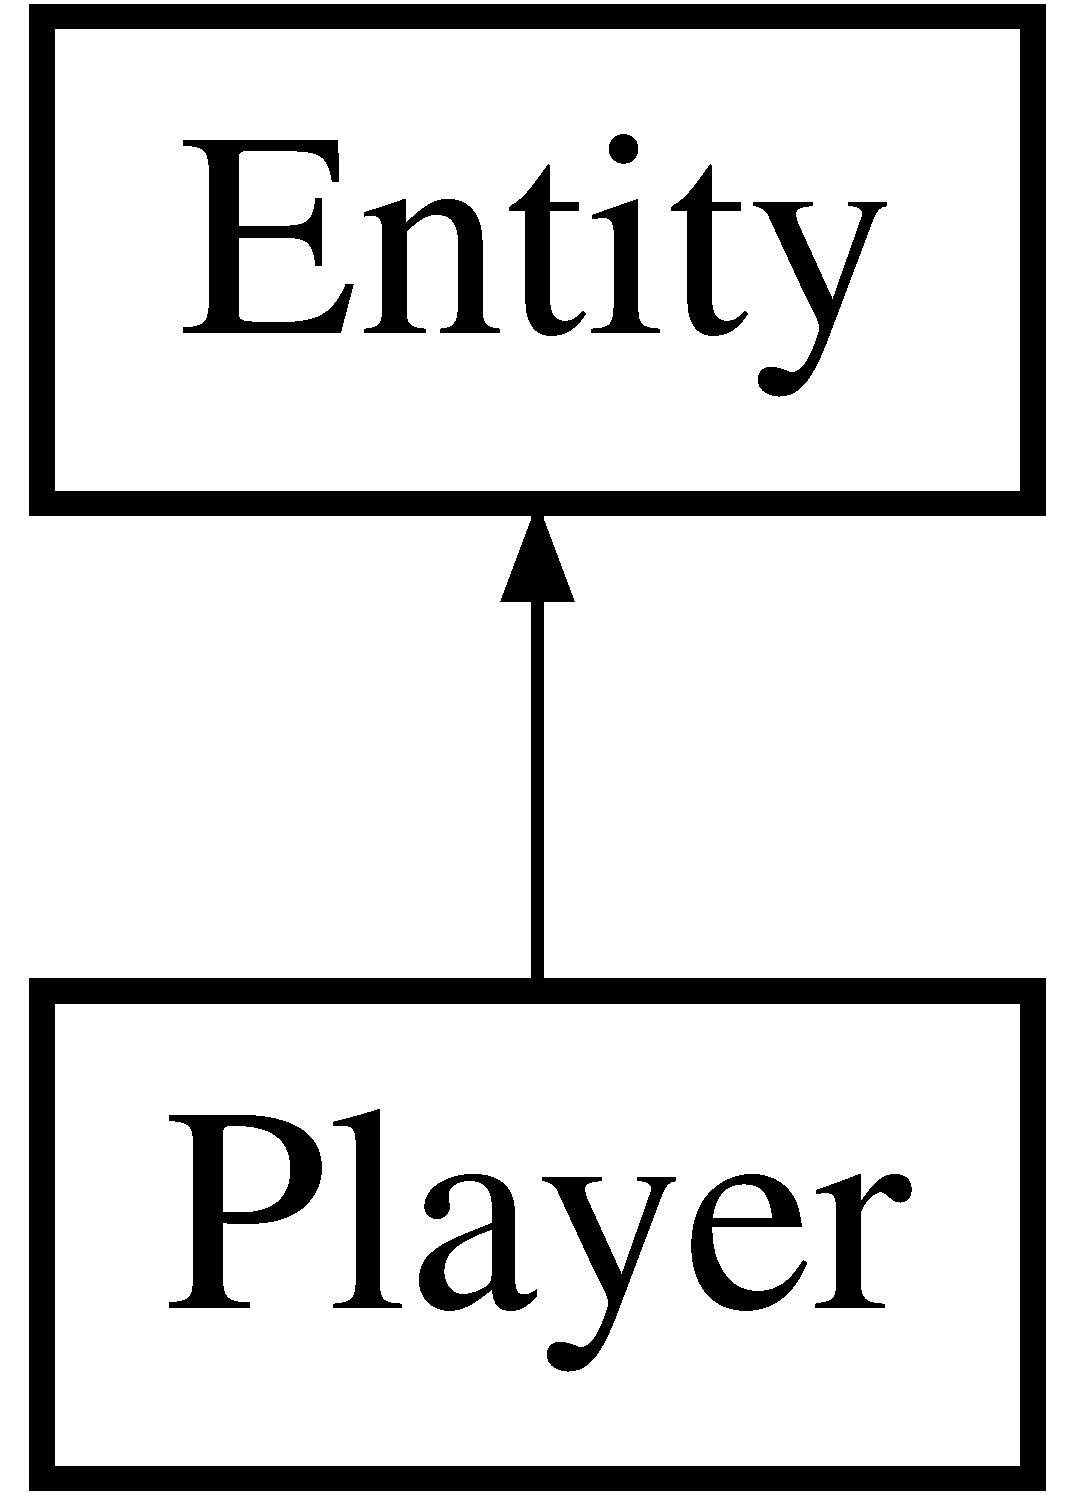
\includegraphics[height=2.000000cm]{class_player}
\end{center}
\end{figure}
\subsection*{Public Member Functions}
\begin{DoxyCompactItemize}
\item 
\hyperlink{class_player_afa77ee030e5d4e529de48e678800a173}{Player} (Vector2f \hyperlink{class_entity_a6af9d6498134ad0906011778bc5736db}{position}, Vector2f \hyperlink{class_entity_ae9a0a364c85f91ade5088b3610131417}{size}, \hyperlink{class_cursor}{Cursor} \&c, \hyperlink{struct_controls_input}{Controls\+Input} \&\hyperlink{classcontrols_input}{controls\+Input}, bool \hyperlink{class_entity_af1b0754c9d5f4afa73834b23c6437101}{is\+Solid}=false, int \hyperlink{class_entity_a4edd9cc2506add0d9e27fade0bf957e8}{state}=0)
\item 
void \hyperlink{class_player_a6912bb6e48efb5845d59f0f4582827ef}{update} () override
\begin{DoxyCompactList}\small\item\em updates player position and rotation \end{DoxyCompactList}\item 
void \hyperlink{class_player_ad39abceb9ff5c7c189010f87d6b46dea}{rotate} ()
\begin{DoxyCompactList}\small\item\em rotates player \end{DoxyCompactList}\item 
void \hyperlink{class_player_a27ca9082a531285731af05f9395ffee8}{draw} (Render\+Window \&window) override
\begin{DoxyCompactList}\small\item\em draws player \end{DoxyCompactList}\item 
\hyperlink{class_entity}{Entity} $\ast$ \hyperlink{class_player_a089d9293cc3be7e5d6d7c89b49538134}{hit} () override
\begin{DoxyCompactList}\small\item\em checks whether the player has been hit \end{DoxyCompactList}\item 
Vector2f \hyperlink{class_player_a59cfaac9d09b12a290d2e89ca656be49}{get\+Pos} () override
\begin{DoxyCompactList}\small\item\em returns vector2f position of player \end{DoxyCompactList}\item 
void \hyperlink{class_player_a14d08591258cea6406002cda8a075917}{Trigger\+Death} ()
\begin{DoxyCompactList}\small\item\em kills the player \end{DoxyCompactList}\item 
void \hyperlink{class_player_aa1452815f38bc6b069f2fda6819b2887}{Trigger\+Life} ()
\begin{DoxyCompactList}\small\item\em revives the player \end{DoxyCompactList}\item 
bool \hyperlink{class_player_a2c1775f5add97e680e7cd538e8dddda3}{collides\+With} (\hyperlink{class_entity}{Entity} $\ast$other)
\begin{DoxyCompactList}\small\item\em checks whether the player is colliding \end{DoxyCompactList}\item 
void \hyperlink{class_player_acf54fe649339974ec2f990f2f484dc3d}{set\+Sprite} (std\+::string path)
\end{DoxyCompactItemize}
\subsection*{Public Attributes}
\begin{DoxyCompactItemize}
\item 
float \hyperlink{class_player_ad94d3e5ab67795f8f848a7fd565f376f}{rotation}
\item 
\hyperlink{struct_player_stats}{Player\+Stats} \hyperlink{class_player_af9bb9d1de3b674a869b2c58b702e9036}{stats}
\item 
\hyperlink{class_hud}{Hud} \hyperlink{class_player_a53a16e90cfe0982879f2f993ee2c7e88}{hud} = \hyperlink{class_hud}{Hud}(\hyperlink{class_player_af9bb9d1de3b674a869b2c58b702e9036}{stats})
\end{DoxyCompactItemize}
\subsection*{Additional Inherited Members}


\subsection{Detailed Description}
Handles player movement, interaction, animations and art. 

Definition at line 21 of file Player.\+h.



\subsection{Constructor \& Destructor Documentation}
\mbox{\Hypertarget{class_player_afa77ee030e5d4e529de48e678800a173}\label{class_player_afa77ee030e5d4e529de48e678800a173}} 
\index{Player@{Player}!Player@{Player}}
\index{Player@{Player}!Player@{Player}}
\subsubsection{\texorpdfstring{Player()}{Player()}}
{\footnotesize\ttfamily Player\+::\+Player (\begin{DoxyParamCaption}\item[{Vector2f}]{position,  }\item[{Vector2f}]{size,  }\item[{\hyperlink{class_cursor}{Cursor} \&}]{c,  }\item[{\hyperlink{struct_controls_input}{Controls\+Input} \&}]{controls\+Input,  }\item[{bool}]{is\+Solid = {\ttfamily false},  }\item[{int}]{state = {\ttfamily 0} }\end{DoxyParamCaption})}



Definition at line 5 of file Player.\+cpp.



\subsection{Member Function Documentation}
\mbox{\Hypertarget{class_player_a2c1775f5add97e680e7cd538e8dddda3}\label{class_player_a2c1775f5add97e680e7cd538e8dddda3}} 
\index{Player@{Player}!collides\+With@{collides\+With}}
\index{collides\+With@{collides\+With}!Player@{Player}}
\subsubsection{\texorpdfstring{collides\+With()}{collidesWith()}}
{\footnotesize\ttfamily bool Player\+::collides\+With (\begin{DoxyParamCaption}\item[{\hyperlink{class_entity}{Entity} $\ast$}]{other }\end{DoxyParamCaption})}



checks whether the player is colliding 

\hyperlink{class_player_a2c1775f5add97e680e7cd538e8dddda3}{collides\+With(\+Entity$\ast$ other)} 

Definition at line 57 of file Player.\+cpp.

\mbox{\Hypertarget{class_player_a27ca9082a531285731af05f9395ffee8}\label{class_player_a27ca9082a531285731af05f9395ffee8}} 
\index{Player@{Player}!draw@{draw}}
\index{draw@{draw}!Player@{Player}}
\subsubsection{\texorpdfstring{draw()}{draw()}}
{\footnotesize\ttfamily void Player\+::draw (\begin{DoxyParamCaption}\item[{Render\+Window \&}]{window }\end{DoxyParamCaption})\hspace{0.3cm}{\ttfamily [override]}, {\ttfamily [virtual]}}



draws player 

\hyperlink{class_player_a27ca9082a531285731af05f9395ffee8}{draw()} 

Reimplemented from \hyperlink{class_entity_a030c3aa6641df7981a2d8a3fba890ec7}{Entity}.



Definition at line 30 of file Player.\+cpp.

\mbox{\Hypertarget{class_player_a59cfaac9d09b12a290d2e89ca656be49}\label{class_player_a59cfaac9d09b12a290d2e89ca656be49}} 
\index{Player@{Player}!get\+Pos@{get\+Pos}}
\index{get\+Pos@{get\+Pos}!Player@{Player}}
\subsubsection{\texorpdfstring{get\+Pos()}{getPos()}}
{\footnotesize\ttfamily Vector2f Player\+::get\+Pos (\begin{DoxyParamCaption}{ }\end{DoxyParamCaption})\hspace{0.3cm}{\ttfamily [override]}, {\ttfamily [virtual]}}



returns vector2f position of player 

\hyperlink{class_player_a59cfaac9d09b12a290d2e89ca656be49}{get\+Pos()} 

Reimplemented from \hyperlink{class_entity_a8b6080f0ab76702fcd00108aef8ea9dd}{Entity}.



Definition at line 39 of file Player.\+cpp.

\mbox{\Hypertarget{class_player_a089d9293cc3be7e5d6d7c89b49538134}\label{class_player_a089d9293cc3be7e5d6d7c89b49538134}} 
\index{Player@{Player}!hit@{hit}}
\index{hit@{hit}!Player@{Player}}
\subsubsection{\texorpdfstring{hit()}{hit()}}
{\footnotesize\ttfamily \hyperlink{class_entity}{Entity} $\ast$ Player\+::hit (\begin{DoxyParamCaption}{ }\end{DoxyParamCaption})\hspace{0.3cm}{\ttfamily [override]}, {\ttfamily [virtual]}}



checks whether the player has been hit 

\hyperlink{class_player_a089d9293cc3be7e5d6d7c89b49538134}{hit()} 

Reimplemented from \hyperlink{class_entity_a29117f3f40e7069d5d4c1b2fca7819d6}{Entity}.



Definition at line 35 of file Player.\+cpp.

\mbox{\Hypertarget{class_player_ad39abceb9ff5c7c189010f87d6b46dea}\label{class_player_ad39abceb9ff5c7c189010f87d6b46dea}} 
\index{Player@{Player}!rotate@{rotate}}
\index{rotate@{rotate}!Player@{Player}}
\subsubsection{\texorpdfstring{rotate()}{rotate()}}
{\footnotesize\ttfamily void Player\+::rotate (\begin{DoxyParamCaption}{ }\end{DoxyParamCaption})}



rotates player 

\hyperlink{class_player_ad39abceb9ff5c7c189010f87d6b46dea}{rotate()} 

Definition at line 20 of file Player.\+cpp.

\mbox{\Hypertarget{class_player_acf54fe649339974ec2f990f2f484dc3d}\label{class_player_acf54fe649339974ec2f990f2f484dc3d}} 
\index{Player@{Player}!set\+Sprite@{set\+Sprite}}
\index{set\+Sprite@{set\+Sprite}!Player@{Player}}
\subsubsection{\texorpdfstring{set\+Sprite()}{setSprite()}}
{\footnotesize\ttfamily void Player\+::set\+Sprite (\begin{DoxyParamCaption}\item[{std\+::string}]{path }\end{DoxyParamCaption})}



Definition at line 62 of file Player.\+cpp.

\mbox{\Hypertarget{class_player_a14d08591258cea6406002cda8a075917}\label{class_player_a14d08591258cea6406002cda8a075917}} 
\index{Player@{Player}!Trigger\+Death@{Trigger\+Death}}
\index{Trigger\+Death@{Trigger\+Death}!Player@{Player}}
\subsubsection{\texorpdfstring{Trigger\+Death()}{TriggerDeath()}}
{\footnotesize\ttfamily void Player\+::\+Trigger\+Death (\begin{DoxyParamCaption}{ }\end{DoxyParamCaption})}



kills the player 

\hyperlink{class_player_a14d08591258cea6406002cda8a075917}{Trigger\+Death()} 

Definition at line 44 of file Player.\+cpp.

\mbox{\Hypertarget{class_player_aa1452815f38bc6b069f2fda6819b2887}\label{class_player_aa1452815f38bc6b069f2fda6819b2887}} 
\index{Player@{Player}!Trigger\+Life@{Trigger\+Life}}
\index{Trigger\+Life@{Trigger\+Life}!Player@{Player}}
\subsubsection{\texorpdfstring{Trigger\+Life()}{TriggerLife()}}
{\footnotesize\ttfamily void Player\+::\+Trigger\+Life (\begin{DoxyParamCaption}{ }\end{DoxyParamCaption})}



revives the player 

\hyperlink{class_player_aa1452815f38bc6b069f2fda6819b2887}{Trigger\+Life()} 

Definition at line 51 of file Player.\+cpp.

\mbox{\Hypertarget{class_player_a6912bb6e48efb5845d59f0f4582827ef}\label{class_player_a6912bb6e48efb5845d59f0f4582827ef}} 
\index{Player@{Player}!update@{update}}
\index{update@{update}!Player@{Player}}
\subsubsection{\texorpdfstring{update()}{update()}}
{\footnotesize\ttfamily void Player\+::update (\begin{DoxyParamCaption}{ }\end{DoxyParamCaption})\hspace{0.3cm}{\ttfamily [override]}, {\ttfamily [virtual]}}



updates player position and rotation 

\hyperlink{class_player_a6912bb6e48efb5845d59f0f4582827ef}{update()} 

Reimplemented from \hyperlink{class_entity_aed73e98b980b85833428c935cc1c69f8}{Entity}.



Definition at line 12 of file Player.\+cpp.



\subsection{Member Data Documentation}
\mbox{\Hypertarget{class_player_a53a16e90cfe0982879f2f993ee2c7e88}\label{class_player_a53a16e90cfe0982879f2f993ee2c7e88}} 
\index{Player@{Player}!hud@{hud}}
\index{hud@{hud}!Player@{Player}}
\subsubsection{\texorpdfstring{hud}{hud}}
{\footnotesize\ttfamily \hyperlink{class_hud}{Hud} Player\+::hud = \hyperlink{class_hud}{Hud}(\hyperlink{class_player_af9bb9d1de3b674a869b2c58b702e9036}{stats})}



Definition at line 35 of file Player.\+h.

\mbox{\Hypertarget{class_player_ad94d3e5ab67795f8f848a7fd565f376f}\label{class_player_ad94d3e5ab67795f8f848a7fd565f376f}} 
\index{Player@{Player}!rotation@{rotation}}
\index{rotation@{rotation}!Player@{Player}}
\subsubsection{\texorpdfstring{rotation}{rotation}}
{\footnotesize\ttfamily float Player\+::rotation}

Rotation in degrees to rotate the player sprite 

Definition at line 32 of file Player.\+h.

\mbox{\Hypertarget{class_player_af9bb9d1de3b674a869b2c58b702e9036}\label{class_player_af9bb9d1de3b674a869b2c58b702e9036}} 
\index{Player@{Player}!stats@{stats}}
\index{stats@{stats}!Player@{Player}}
\subsubsection{\texorpdfstring{stats}{stats}}
{\footnotesize\ttfamily \hyperlink{struct_player_stats}{Player\+Stats} Player\+::stats}



Definition at line 33 of file Player.\+h.



The documentation for this class was generated from the following files\+:\begin{DoxyCompactItemize}
\item 
C\+:/\+Users/joost/\+Documents/\+Git\+Hub/topdown/\+Code/\+Team\+Topdown/\+Team\+Topdown/\hyperlink{_player_8h}{Player.\+h}\item 
C\+:/\+Users/joost/\+Documents/\+Git\+Hub/topdown/\+Code/\+Team\+Topdown/\+Team\+Topdown/\hyperlink{_player_8cpp}{Player.\+cpp}\end{DoxyCompactItemize}

\hypertarget{struct_player_stats}{}\section{Player\+Stats Class Reference}
\label{struct_player_stats}\index{Player\+Stats@{Player\+Stats}}


Struct that contains player statistics.  




{\ttfamily \#include $<$Player\+Stats.\+h$>$}

\subsection*{Public Member Functions}
\begin{DoxyCompactItemize}
\item 
\hyperlink{struct_player_stats_a80dcf207b4271ad8e3e8e3766b52a4eb}{Player\+Stats} ()
\item 
void \hyperlink{struct_player_stats_a142ec7949841369d22ea4d6e7fa78caf}{Reset} ()
\end{DoxyCompactItemize}
\subsection*{Public Attributes}
\begin{DoxyCompactItemize}
\item 
Vector2f \hyperlink{struct_player_stats_a69d3f79697de6ab61e0e623bcc2149d7}{position} = Vector2f(0, 0)
\item 
bool \hyperlink{struct_player_stats_a407c02f77b9057c2dc2405fda01ffc10}{dodging} = false
\item 
int \hyperlink{struct_player_stats_a8290edfa2a4f9c07952a463a2130b854}{pause\+Menu\+Open} = 0
\item 
float \hyperlink{struct_player_stats_a4f410ca507dc427d07216c4d9f5c72b4}{melee\+Range} = 40
\item 
float \hyperlink{struct_player_stats_a42bf3bb543b6a0b2795e2da227f61a8f}{melee\+Speed} = 15
\item 
\hyperlink{struct_timer}{Timer} \hyperlink{struct_player_stats_ae27c978afce4840051663616408251ea}{energy}
\item 
\hyperlink{struct_timer}{Timer} \hyperlink{struct_player_stats_a22cc49283aedec58d7ff532dc50e1541}{sprint}
\item 
\hyperlink{struct_timer}{Timer} \hyperlink{struct_player_stats_a55071f370b68104e5ee0c3d56ee6e9a4}{dodge}
\item 
\hyperlink{struct_timer}{Timer} \hyperlink{struct_player_stats_a261129c34a506778d0b83ed5857263b6}{shoot}
\item 
\hyperlink{struct_timer}{Timer} \hyperlink{struct_player_stats_a0f20347dec48b0df3ab77156b9535063}{reload}
\item 
\hyperlink{struct_timer}{Timer} \hyperlink{struct_player_stats_ac30ff0f8390f54929be9f378cd759c81}{seconds}
\item 
int \hyperlink{struct_player_stats_abfb2168c91b0bbcf5a0b996b0bf7d1c7}{stamina} = 100
\item 
float \hyperlink{struct_player_stats_a19d6791dea891e37558e940dc486fef4}{speed} = 3
\item 
int \hyperlink{struct_player_stats_a2600a3f6f284a3eeddcc080953e90dfa}{ammo} = 5
\item 
int \hyperlink{struct_player_stats_afbfb80a6992ad7a4627e62ce89b20a10}{max\+Ammo} = 5
\item 
int \hyperlink{struct_player_stats_a8a20827747238fa6322e7d79a4f46f51}{is\+Dead} = 0
\item 
int \hyperlink{struct_player_stats_a42b7d05fe86a26230ff2b55bbe0489ad}{remaining\+Time} = 120
\item 
int \hyperlink{struct_player_stats_ad58078805e9b2f5978639b2aa7447e81}{start\+Time} = 120
\end{DoxyCompactItemize}


\subsection{Detailed Description}
Struct that contains player statistics. 

Definition at line 13 of file Player\+Stats.\+h.



\subsection{Constructor \& Destructor Documentation}
\mbox{\Hypertarget{struct_player_stats_a80dcf207b4271ad8e3e8e3766b52a4eb}\label{struct_player_stats_a80dcf207b4271ad8e3e8e3766b52a4eb}} 
\index{Player\+Stats@{Player\+Stats}!Player\+Stats@{Player\+Stats}}
\index{Player\+Stats@{Player\+Stats}!Player\+Stats@{Player\+Stats}}
\subsubsection{\texorpdfstring{Player\+Stats()}{PlayerStats()}}
{\footnotesize\ttfamily Player\+Stats\+::\+Player\+Stats (\begin{DoxyParamCaption}{ }\end{DoxyParamCaption})}



Definition at line 5 of file Player\+Stats.\+cpp.



\subsection{Member Function Documentation}
\mbox{\Hypertarget{struct_player_stats_a142ec7949841369d22ea4d6e7fa78caf}\label{struct_player_stats_a142ec7949841369d22ea4d6e7fa78caf}} 
\index{Player\+Stats@{Player\+Stats}!Reset@{Reset}}
\index{Reset@{Reset}!Player\+Stats@{Player\+Stats}}
\subsubsection{\texorpdfstring{Reset()}{Reset()}}
{\footnotesize\ttfamily void Player\+Stats\+::\+Reset (\begin{DoxyParamCaption}{ }\end{DoxyParamCaption})}

$<$ player max stamina

$<$ player max speed

$<$ \char`\"{}is player dodging?\char`\"{} boolean

$<$ current gun ammunition

$<$ player dead state 

Definition at line 15 of file Player\+Stats.\+cpp.



\subsection{Member Data Documentation}
\mbox{\Hypertarget{struct_player_stats_a2600a3f6f284a3eeddcc080953e90dfa}\label{struct_player_stats_a2600a3f6f284a3eeddcc080953e90dfa}} 
\index{Player\+Stats@{Player\+Stats}!ammo@{ammo}}
\index{ammo@{ammo}!Player\+Stats@{Player\+Stats}}
\subsubsection{\texorpdfstring{ammo}{ammo}}
{\footnotesize\ttfamily int Player\+Stats\+::ammo = 5}

current gun ammunition 

Definition at line 34 of file Player\+Stats.\+h.

\mbox{\Hypertarget{struct_player_stats_a55071f370b68104e5ee0c3d56ee6e9a4}\label{struct_player_stats_a55071f370b68104e5ee0c3d56ee6e9a4}} 
\index{Player\+Stats@{Player\+Stats}!dodge@{dodge}}
\index{dodge@{dodge}!Player\+Stats@{Player\+Stats}}
\subsubsection{\texorpdfstring{dodge}{dodge}}
{\footnotesize\ttfamily \hyperlink{struct_timer}{Timer} Player\+Stats\+::dodge}



Definition at line 27 of file Player\+Stats.\+h.

\mbox{\Hypertarget{struct_player_stats_a407c02f77b9057c2dc2405fda01ffc10}\label{struct_player_stats_a407c02f77b9057c2dc2405fda01ffc10}} 
\index{Player\+Stats@{Player\+Stats}!dodging@{dodging}}
\index{dodging@{dodging}!Player\+Stats@{Player\+Stats}}
\subsubsection{\texorpdfstring{dodging}{dodging}}
{\footnotesize\ttfamily bool Player\+Stats\+::dodging = false}

\char`\"{}is player dodging?\char`\"{} boolean 

Definition at line 19 of file Player\+Stats.\+h.

\mbox{\Hypertarget{struct_player_stats_ae27c978afce4840051663616408251ea}\label{struct_player_stats_ae27c978afce4840051663616408251ea}} 
\index{Player\+Stats@{Player\+Stats}!energy@{energy}}
\index{energy@{energy}!Player\+Stats@{Player\+Stats}}
\subsubsection{\texorpdfstring{energy}{energy}}
{\footnotesize\ttfamily \hyperlink{struct_timer}{Timer} Player\+Stats\+::energy}



Definition at line 27 of file Player\+Stats.\+h.

\mbox{\Hypertarget{struct_player_stats_a8a20827747238fa6322e7d79a4f46f51}\label{struct_player_stats_a8a20827747238fa6322e7d79a4f46f51}} 
\index{Player\+Stats@{Player\+Stats}!is\+Dead@{is\+Dead}}
\index{is\+Dead@{is\+Dead}!Player\+Stats@{Player\+Stats}}
\subsubsection{\texorpdfstring{is\+Dead}{isDead}}
{\footnotesize\ttfamily int Player\+Stats\+::is\+Dead = 0}

player dead state 

Definition at line 36 of file Player\+Stats.\+h.

\mbox{\Hypertarget{struct_player_stats_afbfb80a6992ad7a4627e62ce89b20a10}\label{struct_player_stats_afbfb80a6992ad7a4627e62ce89b20a10}} 
\index{Player\+Stats@{Player\+Stats}!max\+Ammo@{max\+Ammo}}
\index{max\+Ammo@{max\+Ammo}!Player\+Stats@{Player\+Stats}}
\subsubsection{\texorpdfstring{max\+Ammo}{maxAmmo}}
{\footnotesize\ttfamily int Player\+Stats\+::max\+Ammo = 5}



Definition at line 35 of file Player\+Stats.\+h.

\mbox{\Hypertarget{struct_player_stats_a4f410ca507dc427d07216c4d9f5c72b4}\label{struct_player_stats_a4f410ca507dc427d07216c4d9f5c72b4}} 
\index{Player\+Stats@{Player\+Stats}!melee\+Range@{melee\+Range}}
\index{melee\+Range@{melee\+Range}!Player\+Stats@{Player\+Stats}}
\subsubsection{\texorpdfstring{melee\+Range}{meleeRange}}
{\footnotesize\ttfamily float Player\+Stats\+::melee\+Range = 40}



Definition at line 21 of file Player\+Stats.\+h.

\mbox{\Hypertarget{struct_player_stats_a42bf3bb543b6a0b2795e2da227f61a8f}\label{struct_player_stats_a42bf3bb543b6a0b2795e2da227f61a8f}} 
\index{Player\+Stats@{Player\+Stats}!melee\+Speed@{melee\+Speed}}
\index{melee\+Speed@{melee\+Speed}!Player\+Stats@{Player\+Stats}}
\subsubsection{\texorpdfstring{melee\+Speed}{meleeSpeed}}
{\footnotesize\ttfamily float Player\+Stats\+::melee\+Speed = 15}



Definition at line 22 of file Player\+Stats.\+h.

\mbox{\Hypertarget{struct_player_stats_a8290edfa2a4f9c07952a463a2130b854}\label{struct_player_stats_a8290edfa2a4f9c07952a463a2130b854}} 
\index{Player\+Stats@{Player\+Stats}!pause\+Menu\+Open@{pause\+Menu\+Open}}
\index{pause\+Menu\+Open@{pause\+Menu\+Open}!Player\+Stats@{Player\+Stats}}
\subsubsection{\texorpdfstring{pause\+Menu\+Open}{pauseMenuOpen}}
{\footnotesize\ttfamily int Player\+Stats\+::pause\+Menu\+Open = 0}



Definition at line 20 of file Player\+Stats.\+h.

\mbox{\Hypertarget{struct_player_stats_a69d3f79697de6ab61e0e623bcc2149d7}\label{struct_player_stats_a69d3f79697de6ab61e0e623bcc2149d7}} 
\index{Player\+Stats@{Player\+Stats}!position@{position}}
\index{position@{position}!Player\+Stats@{Player\+Stats}}
\subsubsection{\texorpdfstring{position}{position}}
{\footnotesize\ttfamily Vector2f Player\+Stats\+::position = Vector2f(0, 0)}



Definition at line 18 of file Player\+Stats.\+h.

\mbox{\Hypertarget{struct_player_stats_a0f20347dec48b0df3ab77156b9535063}\label{struct_player_stats_a0f20347dec48b0df3ab77156b9535063}} 
\index{Player\+Stats@{Player\+Stats}!reload@{reload}}
\index{reload@{reload}!Player\+Stats@{Player\+Stats}}
\subsubsection{\texorpdfstring{reload}{reload}}
{\footnotesize\ttfamily \hyperlink{struct_timer}{Timer} Player\+Stats\+::reload}



Definition at line 27 of file Player\+Stats.\+h.

\mbox{\Hypertarget{struct_player_stats_a42b7d05fe86a26230ff2b55bbe0489ad}\label{struct_player_stats_a42b7d05fe86a26230ff2b55bbe0489ad}} 
\index{Player\+Stats@{Player\+Stats}!remaining\+Time@{remaining\+Time}}
\index{remaining\+Time@{remaining\+Time}!Player\+Stats@{Player\+Stats}}
\subsubsection{\texorpdfstring{remaining\+Time}{remainingTime}}
{\footnotesize\ttfamily int Player\+Stats\+::remaining\+Time = 120}



Definition at line 37 of file Player\+Stats.\+h.

\mbox{\Hypertarget{struct_player_stats_ac30ff0f8390f54929be9f378cd759c81}\label{struct_player_stats_ac30ff0f8390f54929be9f378cd759c81}} 
\index{Player\+Stats@{Player\+Stats}!seconds@{seconds}}
\index{seconds@{seconds}!Player\+Stats@{Player\+Stats}}
\subsubsection{\texorpdfstring{seconds}{seconds}}
{\footnotesize\ttfamily \hyperlink{struct_timer}{Timer} Player\+Stats\+::seconds}

timer for player based on fps 

Definition at line 27 of file Player\+Stats.\+h.

\mbox{\Hypertarget{struct_player_stats_a261129c34a506778d0b83ed5857263b6}\label{struct_player_stats_a261129c34a506778d0b83ed5857263b6}} 
\index{Player\+Stats@{Player\+Stats}!shoot@{shoot}}
\index{shoot@{shoot}!Player\+Stats@{Player\+Stats}}
\subsubsection{\texorpdfstring{shoot}{shoot}}
{\footnotesize\ttfamily \hyperlink{struct_timer}{Timer} Player\+Stats\+::shoot}



Definition at line 27 of file Player\+Stats.\+h.

\mbox{\Hypertarget{struct_player_stats_a19d6791dea891e37558e940dc486fef4}\label{struct_player_stats_a19d6791dea891e37558e940dc486fef4}} 
\index{Player\+Stats@{Player\+Stats}!speed@{speed}}
\index{speed@{speed}!Player\+Stats@{Player\+Stats}}
\subsubsection{\texorpdfstring{speed}{speed}}
{\footnotesize\ttfamily float Player\+Stats\+::speed = 3}

player max speed 

Definition at line 33 of file Player\+Stats.\+h.

\mbox{\Hypertarget{struct_player_stats_a22cc49283aedec58d7ff532dc50e1541}\label{struct_player_stats_a22cc49283aedec58d7ff532dc50e1541}} 
\index{Player\+Stats@{Player\+Stats}!sprint@{sprint}}
\index{sprint@{sprint}!Player\+Stats@{Player\+Stats}}
\subsubsection{\texorpdfstring{sprint}{sprint}}
{\footnotesize\ttfamily \hyperlink{struct_timer}{Timer} Player\+Stats\+::sprint}



Definition at line 27 of file Player\+Stats.\+h.

\mbox{\Hypertarget{struct_player_stats_abfb2168c91b0bbcf5a0b996b0bf7d1c7}\label{struct_player_stats_abfb2168c91b0bbcf5a0b996b0bf7d1c7}} 
\index{Player\+Stats@{Player\+Stats}!stamina@{stamina}}
\index{stamina@{stamina}!Player\+Stats@{Player\+Stats}}
\subsubsection{\texorpdfstring{stamina}{stamina}}
{\footnotesize\ttfamily int Player\+Stats\+::stamina = 100}

player max stamina 

Definition at line 32 of file Player\+Stats.\+h.

\mbox{\Hypertarget{struct_player_stats_ad58078805e9b2f5978639b2aa7447e81}\label{struct_player_stats_ad58078805e9b2f5978639b2aa7447e81}} 
\index{Player\+Stats@{Player\+Stats}!start\+Time@{start\+Time}}
\index{start\+Time@{start\+Time}!Player\+Stats@{Player\+Stats}}
\subsubsection{\texorpdfstring{start\+Time}{startTime}}
{\footnotesize\ttfamily int Player\+Stats\+::start\+Time = 120}



Definition at line 38 of file Player\+Stats.\+h.



The documentation for this class was generated from the following files\+:\begin{DoxyCompactItemize}
\item 
C\+:/\+Users/joost/\+Documents/\+Git\+Hub/topdown/\+Code/\+Team\+Topdown/\+Team\+Topdown/\hyperlink{_player_stats_8h}{Player\+Stats.\+h}\item 
C\+:/\+Users/joost/\+Documents/\+Git\+Hub/topdown/\+Code/\+Team\+Topdown/\+Team\+Topdown/\hyperlink{_player_stats_8cpp}{Player\+Stats.\+cpp}\end{DoxyCompactItemize}

\hypertarget{class_playing_state}{}\section{Playing\+State Class Reference}
\label{class_playing_state}\index{Playing\+State@{Playing\+State}}


The gamestate handling all gameplay.  




{\ttfamily \#include $<$Playing\+State.\+hpp$>$}

Inheritance diagram for Playing\+State\+:\begin{figure}[H]
\begin{center}
\leavevmode
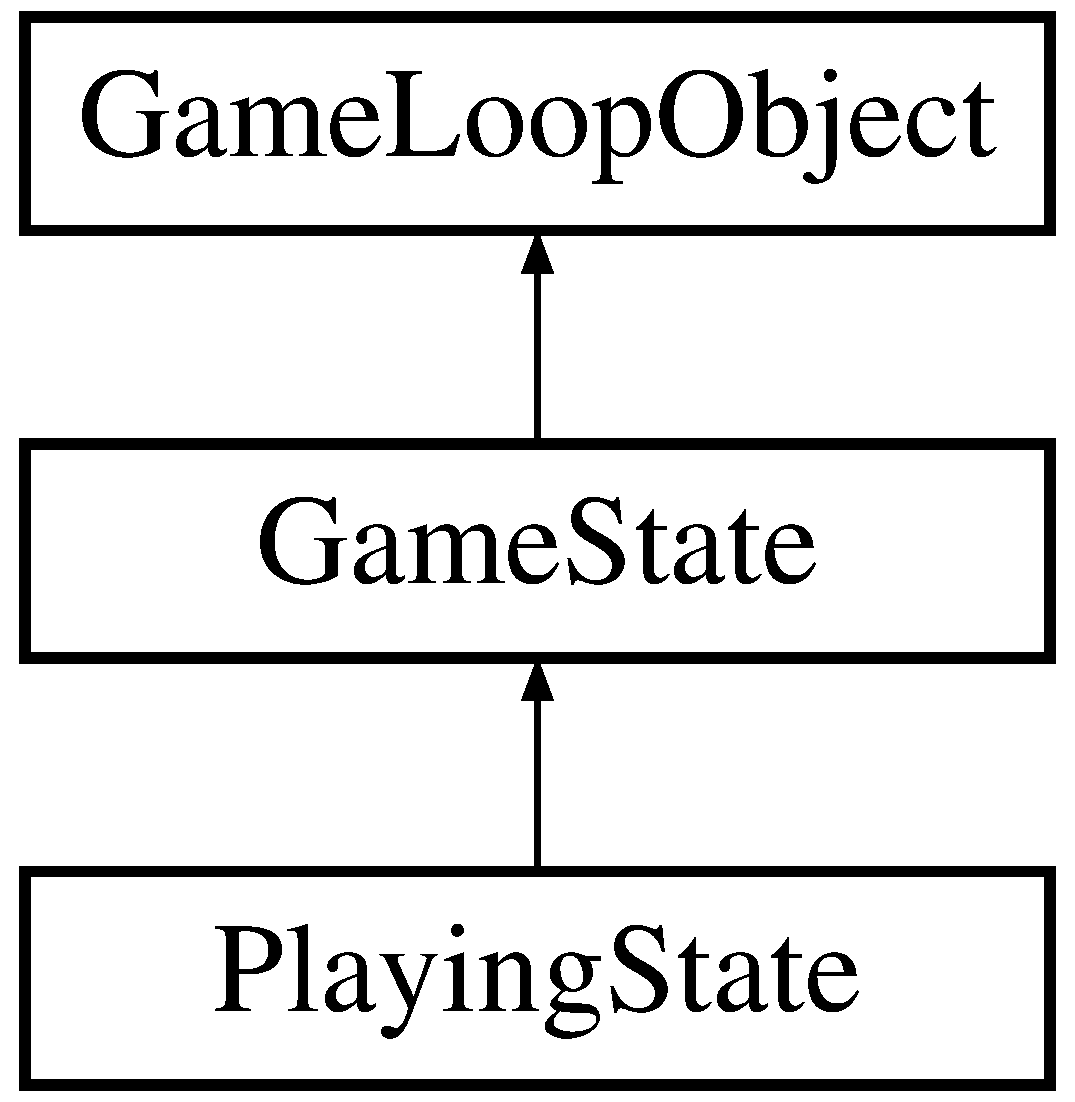
\includegraphics[height=3.000000cm]{class_playing_state}
\end{center}
\end{figure}
\subsection*{Public Member Functions}
\begin{DoxyCompactItemize}
\item 
\hyperlink{class_playing_state_a81610cb256b5a4394200cef8aba82ade}{Playing\+State} (sf\+::\+Render\+Window \&window, \hyperlink{class_game_state_manager}{Game\+State\+Manager} \&gsm, \hyperlink{struct_controls_input}{Controls\+Input} \&ci, \hyperlink{class_level_manager}{Level\+Manager} \&lm, \hyperlink{class_camera}{Camera} \&cm, \hyperlink{class_cursor}{Cursor} \&c, \hyperlink{class_player}{Player} \&p)
\begin{DoxyCompactList}\small\item\em The constructor method of the gamestate handling all gameplay. \end{DoxyCompactList}\item 
void \hyperlink{class_playing_state_ab61fc6f59f00ccf5db80f67d5e4c50a1}{Handle\+Input} ()
\begin{DoxyCompactList}\small\item\em The state\textquotesingle{}s game loop method for handling keyboard and mouse input. \end{DoxyCompactList}\item 
void \hyperlink{class_playing_state_afb7ccd732dfaad4397b5096876092136}{Update} ()
\begin{DoxyCompactList}\small\item\em The state\textquotesingle{}s game loop method for updating the game. \end{DoxyCompactList}\item 
void \hyperlink{class_playing_state_a6f5feffc1c6de994450828fbe2f5c173}{Draw} (sf\+::\+Render\+Window \&window)
\begin{DoxyCompactList}\small\item\em The state\textquotesingle{}s game loop method for drawing on the window. \end{DoxyCompactList}\item 
void \hyperlink{class_playing_state_af3c78b678960f69e5130ca84c1761d1f}{transition\+To\+This} ()
\item 
void \hyperlink{class_playing_state_a15418b49381b61c98d6b9cdc5d3a83d1}{transition\+From\+This} ()
\end{DoxyCompactItemize}


\subsection{Detailed Description}
The gamestate handling all gameplay. 

In this gamestate the player plays the game. Works together with the level manager. The level manager handles the map, entitycontroller and music while the playing state handles everything else (mainly the pause menu, level switching and handling player death (animation and resurrection). 

Definition at line 24 of file Playing\+State.\+hpp.



\subsection{Constructor \& Destructor Documentation}
\mbox{\Hypertarget{class_playing_state_a81610cb256b5a4394200cef8aba82ade}\label{class_playing_state_a81610cb256b5a4394200cef8aba82ade}} 
\index{Playing\+State@{Playing\+State}!Playing\+State@{Playing\+State}}
\index{Playing\+State@{Playing\+State}!Playing\+State@{Playing\+State}}
\subsubsection{\texorpdfstring{Playing\+State()}{PlayingState()}}
{\footnotesize\ttfamily Playing\+State\+::\+Playing\+State (\begin{DoxyParamCaption}\item[{sf\+::\+Render\+Window \&}]{window,  }\item[{\hyperlink{class_game_state_manager}{Game\+State\+Manager} \&}]{gsm,  }\item[{\hyperlink{struct_controls_input}{Controls\+Input} \&}]{ci,  }\item[{\hyperlink{class_level_manager}{Level\+Manager} \&}]{lm,  }\item[{\hyperlink{class_camera}{Camera} \&}]{cm,  }\item[{\hyperlink{class_cursor}{Cursor} \&}]{c,  }\item[{\hyperlink{class_player}{Player} \&}]{p }\end{DoxyParamCaption})}



The constructor method of the gamestate handling all gameplay. 

Requires a window to draw on, the gamestatemanager to switch states, controlsinput to read keyboard and mouse input, the level manager for handling the map, entitycontroller and music, the camera to follow the player, the cursor (crosshair) and the player. 

Definition at line 6 of file Playing\+State.\+cpp.



\subsection{Member Function Documentation}
\mbox{\Hypertarget{class_playing_state_a6f5feffc1c6de994450828fbe2f5c173}\label{class_playing_state_a6f5feffc1c6de994450828fbe2f5c173}} 
\index{Playing\+State@{Playing\+State}!Draw@{Draw}}
\index{Draw@{Draw}!Playing\+State@{Playing\+State}}
\subsubsection{\texorpdfstring{Draw()}{Draw()}}
{\footnotesize\ttfamily void Playing\+State\+::\+Draw (\begin{DoxyParamCaption}\item[{sf\+::\+Render\+Window \&}]{window }\end{DoxyParamCaption})\hspace{0.3cm}{\ttfamily [virtual]}}



The state\textquotesingle{}s game loop method for drawing on the window. 

Draws everything gameplay related to the screen. 

Reimplemented from \hyperlink{class_game_state_a8741c5c696c6c366beb4b845c08c3cf8}{Game\+State}.



Definition at line 171 of file Playing\+State.\+cpp.

\mbox{\Hypertarget{class_playing_state_ab61fc6f59f00ccf5db80f67d5e4c50a1}\label{class_playing_state_ab61fc6f59f00ccf5db80f67d5e4c50a1}} 
\index{Playing\+State@{Playing\+State}!Handle\+Input@{Handle\+Input}}
\index{Handle\+Input@{Handle\+Input}!Playing\+State@{Playing\+State}}
\subsubsection{\texorpdfstring{Handle\+Input()}{HandleInput()}}
{\footnotesize\ttfamily void Playing\+State\+::\+Handle\+Input (\begin{DoxyParamCaption}{ }\end{DoxyParamCaption})\hspace{0.3cm}{\ttfamily [virtual]}}



The state\textquotesingle{}s game loop method for handling keyboard and mouse input. 

Handles all keyboard and mouse input. Pressing Escape opens the pause menu, from which the player can resume, restart the level, return to main menu or quit the game. If the player died, pressing Space will restart the level. 

Reimplemented from \hyperlink{class_game_state_a8bce2828cee99ae7c07322804531fd01}{Game\+State}.



Definition at line 59 of file Playing\+State.\+cpp.

\mbox{\Hypertarget{class_playing_state_a15418b49381b61c98d6b9cdc5d3a83d1}\label{class_playing_state_a15418b49381b61c98d6b9cdc5d3a83d1}} 
\index{Playing\+State@{Playing\+State}!transition\+From\+This@{transition\+From\+This}}
\index{transition\+From\+This@{transition\+From\+This}!Playing\+State@{Playing\+State}}
\subsubsection{\texorpdfstring{transition\+From\+This()}{transitionFromThis()}}
{\footnotesize\ttfamily void Playing\+State\+::transition\+From\+This (\begin{DoxyParamCaption}{ }\end{DoxyParamCaption})}

void transition\+From\+This brief Initiates a screen transition towards the next state. 

Definition at line 216 of file Playing\+State.\+cpp.

\mbox{\Hypertarget{class_playing_state_af3c78b678960f69e5130ca84c1761d1f}\label{class_playing_state_af3c78b678960f69e5130ca84c1761d1f}} 
\index{Playing\+State@{Playing\+State}!transition\+To\+This@{transition\+To\+This}}
\index{transition\+To\+This@{transition\+To\+This}!Playing\+State@{Playing\+State}}
\subsubsection{\texorpdfstring{transition\+To\+This()}{transitionToThis()}}
{\footnotesize\ttfamily void Playing\+State\+::transition\+To\+This (\begin{DoxyParamCaption}{ }\end{DoxyParamCaption})}

void transition\+To\+This /brief Initiates a screen transition when entering this state. 

Definition at line 191 of file Playing\+State.\+cpp.

\mbox{\Hypertarget{class_playing_state_afb7ccd732dfaad4397b5096876092136}\label{class_playing_state_afb7ccd732dfaad4397b5096876092136}} 
\index{Playing\+State@{Playing\+State}!Update@{Update}}
\index{Update@{Update}!Playing\+State@{Playing\+State}}
\subsubsection{\texorpdfstring{Update()}{Update()}}
{\footnotesize\ttfamily void Playing\+State\+::\+Update (\begin{DoxyParamCaption}{ }\end{DoxyParamCaption})\hspace{0.3cm}{\ttfamily [virtual]}}



The state\textquotesingle{}s game loop method for updating the game. 

Updates everything gameplay related. 

Reimplemented from \hyperlink{class_game_state_a5be51b634f95bc6e57066ad6931aa18b}{Game\+State}.



Definition at line 122 of file Playing\+State.\+cpp.



The documentation for this class was generated from the following files\+:\begin{DoxyCompactItemize}
\item 
C\+:/\+Users/joost/\+Documents/\+Git\+Hub/topdown/\+Code/\+Team\+Topdown/\+Team\+Topdown/\hyperlink{_playing_state_8hpp}{Playing\+State.\+hpp}\item 
C\+:/\+Users/joost/\+Documents/\+Git\+Hub/topdown/\+Code/\+Team\+Topdown/\+Team\+Topdown/\hyperlink{_playing_state_8cpp}{Playing\+State.\+cpp}\end{DoxyCompactItemize}

\hypertarget{class_spike}{}\section{Spike Class Reference}
\label{class_spike}\index{Spike@{Spike}}


Set of spikes which protrude and retract based on a timer. A set of spikes which change states every 1/2th second. The initial state is given with our constructor, and pulled from the map by green value. The player is also given as a reference to be able to call the Trigger\+Death() function.  




{\ttfamily \#include $<$Spike.\+h$>$}

Inheritance diagram for Spike\+:\begin{figure}[H]
\begin{center}
\leavevmode
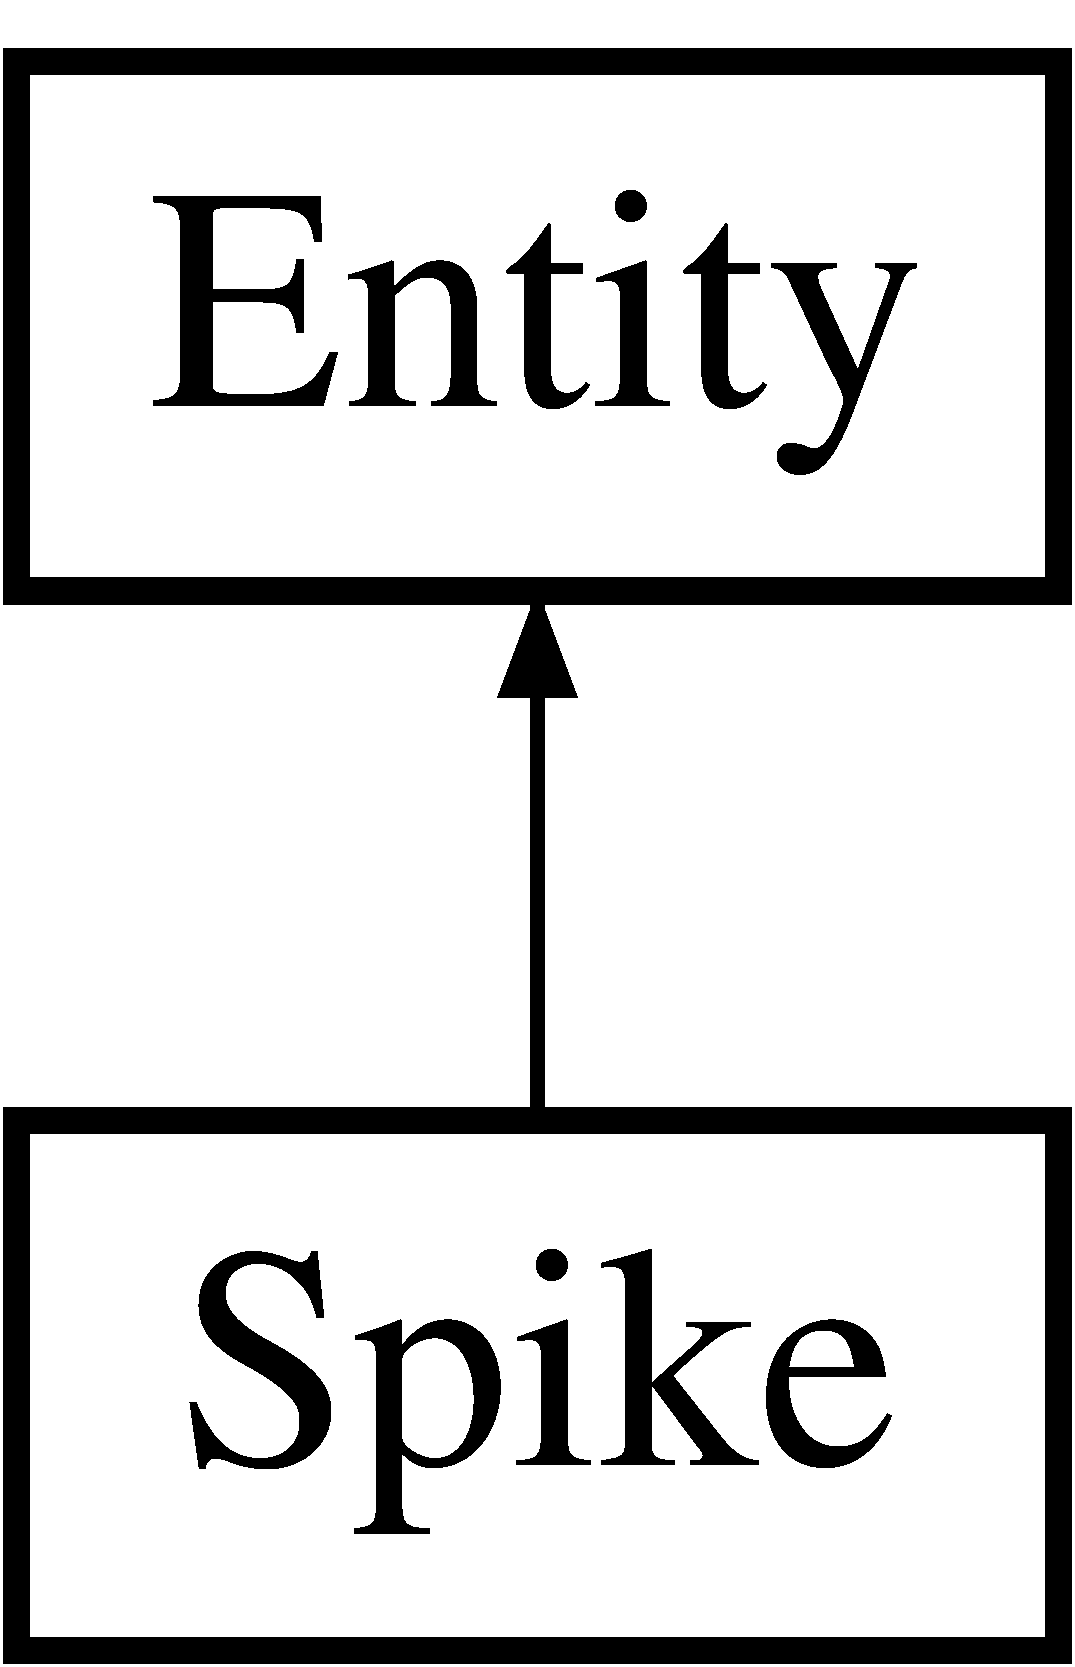
\includegraphics[height=2.000000cm]{class_spike}
\end{center}
\end{figure}
\subsection*{Public Member Functions}
\begin{DoxyCompactItemize}
\item 
\hyperlink{class_spike_a7dd2800abd43bbde613116eded656144}{Spike} (Vector2f \hyperlink{class_entity_a6af9d6498134ad0906011778bc5736db}{position}, unsigned int start\+State, \hyperlink{class_player}{Player} \&p, Vector2f \hyperlink{class_entity_ae9a0a364c85f91ade5088b3610131417}{size}=Vector2f(32.\+0f, 32.\+0f), bool is\+Solid=false)
\item 
void \hyperlink{class_spike_a5f1fc626e9f58f4a08a002c6d2549942}{update} () override
\item 
void \hyperlink{class_spike_a6f1baae74e1b5140459d2a439ad01547}{draw} (Render\+Window \&w)
\end{DoxyCompactItemize}
\subsection*{Additional Inherited Members}


\subsection{Detailed Description}
Set of spikes which protrude and retract based on a timer. A set of spikes which change states every 1/2th second. The initial state is given with our constructor, and pulled from the map by green value. The player is also given as a reference to be able to call the Trigger\+Death() function. 

Definition at line 16 of file Spike.\+h.



\subsection{Constructor \& Destructor Documentation}
\mbox{\Hypertarget{class_spike_a7dd2800abd43bbde613116eded656144}\label{class_spike_a7dd2800abd43bbde613116eded656144}} 
\index{Spike@{Spike}!Spike@{Spike}}
\index{Spike@{Spike}!Spike@{Spike}}
\subsubsection{\texorpdfstring{Spike()}{Spike()}}
{\footnotesize\ttfamily Spike\+::\+Spike (\begin{DoxyParamCaption}\item[{Vector2f}]{position,  }\item[{unsigned int}]{start\+State,  }\item[{\hyperlink{class_player}{Player} \&}]{p,  }\item[{Vector2f}]{size = {\ttfamily Vector2f(32.0f,~32.0f)},  }\item[{bool}]{is\+Solid = {\ttfamily false} }\end{DoxyParamCaption})}



Definition at line 5 of file Spike.\+cpp.



\subsection{Member Function Documentation}
\mbox{\Hypertarget{class_spike_a6f1baae74e1b5140459d2a439ad01547}\label{class_spike_a6f1baae74e1b5140459d2a439ad01547}} 
\index{Spike@{Spike}!draw@{draw}}
\index{draw@{draw}!Spike@{Spike}}
\subsubsection{\texorpdfstring{draw()}{draw()}}
{\footnotesize\ttfamily void Spike\+::draw (\begin{DoxyParamCaption}\item[{Render\+Window \&}]{w }\end{DoxyParamCaption})\hspace{0.3cm}{\ttfamily [virtual]}}



Reimplemented from \hyperlink{class_entity_a030c3aa6641df7981a2d8a3fba890ec7}{Entity}.



Definition at line 41 of file Spike.\+cpp.

\mbox{\Hypertarget{class_spike_a5f1fc626e9f58f4a08a002c6d2549942}\label{class_spike_a5f1fc626e9f58f4a08a002c6d2549942}} 
\index{Spike@{Spike}!update@{update}}
\index{update@{update}!Spike@{Spike}}
\subsubsection{\texorpdfstring{update()}{update()}}
{\footnotesize\ttfamily void Spike\+::update (\begin{DoxyParamCaption}{ }\end{DoxyParamCaption})\hspace{0.3cm}{\ttfamily [override]}, {\ttfamily [virtual]}}



Reimplemented from \hyperlink{class_entity_aed73e98b980b85833428c935cc1c69f8}{Entity}.



Definition at line 12 of file Spike.\+cpp.



The documentation for this class was generated from the following files\+:\begin{DoxyCompactItemize}
\item 
C\+:/\+Users/joost/\+Documents/\+Git\+Hub/topdown/\+Code/\+Team\+Topdown/\+Team\+Topdown/\hyperlink{_spike_8h}{Spike.\+h}\item 
C\+:/\+Users/joost/\+Documents/\+Git\+Hub/topdown/\+Code/\+Team\+Topdown/\+Team\+Topdown/\hyperlink{_spike_8cpp}{Spike.\+cpp}\end{DoxyCompactItemize}

\hypertarget{struct_timer}{}\section{Timer Struct Reference}
\label{struct_timer}\index{Timer@{Timer}}


{\ttfamily \#include $<$Timer.\+h$>$}

\subsection*{Public Member Functions}
\begin{DoxyCompactItemize}
\item 
\hyperlink{struct_timer_a596c0bb8ce30fdad499a62b6653c2e8f}{Timer} (float t=0)
\item 
\hyperlink{struct_timer_a14fa469c4c295c5fa6e66a4ad1092146}{$\sim$\+Timer} ()
\item 
void \hyperlink{struct_timer_a745ad59b5a46744cd871a1129a25d74f}{update} ()
\item 
void \hyperlink{struct_timer_a9020542d73357a4eef512eefaf57524b}{reset} ()
\end{DoxyCompactItemize}
\subsection*{Public Attributes}
\begin{DoxyCompactItemize}
\item 
float \hyperlink{struct_timer_a6b75c3f5ce3277c8bea9c6d9ca96dcd7}{start} = 0
\item 
float \hyperlink{struct_timer_ad6268e1d17cd58eb4caffe2a1e3f00ee}{timer} = 0
\item 
bool \hyperlink{struct_timer_aa460ddd1bec761b68d3b2d460c6e483f}{done} = false
\end{DoxyCompactItemize}


\subsection{Detailed Description}


Definition at line 9 of file Timer.\+h.



\subsection{Constructor \& Destructor Documentation}
\mbox{\Hypertarget{struct_timer_a596c0bb8ce30fdad499a62b6653c2e8f}\label{struct_timer_a596c0bb8ce30fdad499a62b6653c2e8f}} 
\index{Timer@{Timer}!Timer@{Timer}}
\index{Timer@{Timer}!Timer@{Timer}}
\subsubsection{\texorpdfstring{Timer()}{Timer()}}
{\footnotesize\ttfamily Timer\+::\+Timer (\begin{DoxyParamCaption}\item[{float}]{t = {\ttfamily 0} }\end{DoxyParamCaption})}

Sets a fps based timer with duration(frames) t. 60fps = 1 sec 

Definition at line 5 of file Timer.\+cpp.

\mbox{\Hypertarget{struct_timer_a14fa469c4c295c5fa6e66a4ad1092146}\label{struct_timer_a14fa469c4c295c5fa6e66a4ad1092146}} 
\index{Timer@{Timer}!````~Timer@{$\sim$\+Timer}}
\index{````~Timer@{$\sim$\+Timer}!Timer@{Timer}}
\subsubsection{\texorpdfstring{$\sim$\+Timer()}{~Timer()}}
{\footnotesize\ttfamily Timer\+::$\sim$\+Timer (\begin{DoxyParamCaption}{ }\end{DoxyParamCaption})\hspace{0.3cm}{\ttfamily [inline]}}



Definition at line 15 of file Timer.\+h.



\subsection{Member Function Documentation}
\mbox{\Hypertarget{struct_timer_a9020542d73357a4eef512eefaf57524b}\label{struct_timer_a9020542d73357a4eef512eefaf57524b}} 
\index{Timer@{Timer}!reset@{reset}}
\index{reset@{reset}!Timer@{Timer}}
\subsubsection{\texorpdfstring{reset()}{reset()}}
{\footnotesize\ttfamily void Timer\+::reset (\begin{DoxyParamCaption}{ }\end{DoxyParamCaption})}



Definition at line 20 of file Timer.\+cpp.

\mbox{\Hypertarget{struct_timer_a745ad59b5a46744cd871a1129a25d74f}\label{struct_timer_a745ad59b5a46744cd871a1129a25d74f}} 
\index{Timer@{Timer}!update@{update}}
\index{update@{update}!Timer@{Timer}}
\subsubsection{\texorpdfstring{update()}{update()}}
{\footnotesize\ttfamily void Timer\+::update (\begin{DoxyParamCaption}{ }\end{DoxyParamCaption})}



Definition at line 11 of file Timer.\+cpp.



\subsection{Member Data Documentation}
\mbox{\Hypertarget{struct_timer_aa460ddd1bec761b68d3b2d460c6e483f}\label{struct_timer_aa460ddd1bec761b68d3b2d460c6e483f}} 
\index{Timer@{Timer}!done@{done}}
\index{done@{done}!Timer@{Timer}}
\subsubsection{\texorpdfstring{done}{done}}
{\footnotesize\ttfamily bool Timer\+::done = false}

if the timer is done 

Definition at line 12 of file Timer.\+h.

\mbox{\Hypertarget{struct_timer_a6b75c3f5ce3277c8bea9c6d9ca96dcd7}\label{struct_timer_a6b75c3f5ce3277c8bea9c6d9ca96dcd7}} 
\index{Timer@{Timer}!start@{start}}
\index{start@{start}!Timer@{Timer}}
\subsubsection{\texorpdfstring{start}{start}}
{\footnotesize\ttfamily float Timer\+::start = 0}

timer duration 

Definition at line 10 of file Timer.\+h.

\mbox{\Hypertarget{struct_timer_ad6268e1d17cd58eb4caffe2a1e3f00ee}\label{struct_timer_ad6268e1d17cd58eb4caffe2a1e3f00ee}} 
\index{Timer@{Timer}!timer@{timer}}
\index{timer@{timer}!Timer@{Timer}}
\subsubsection{\texorpdfstring{timer}{timer}}
{\footnotesize\ttfamily float Timer\+::timer = 0}

current time of timer 

Definition at line 11 of file Timer.\+h.



The documentation for this struct was generated from the following files\+:\begin{DoxyCompactItemize}
\item 
C\+:/\+Users/joost/\+Documents/\+Git\+Hub/topdown/\+Code/\+Team\+Topdown/\+Team\+Topdown/\hyperlink{_timer_8h}{Timer.\+h}\item 
C\+:/\+Users/joost/\+Documents/\+Git\+Hub/topdown/\+Code/\+Team\+Topdown/\+Team\+Topdown/\hyperlink{_timer_8cpp}{Timer.\+cpp}\end{DoxyCompactItemize}

\hypertarget{class_title_screen_state}{}\section{Title\+Screen\+State Class Reference}
\label{class_title_screen_state}\index{Title\+Screen\+State@{Title\+Screen\+State}}


The gamestate that shows the title screen. The first thing the player sees.  




{\ttfamily \#include $<$Title\+Screen\+State.\+hpp$>$}

Inheritance diagram for Title\+Screen\+State\+:\begin{figure}[H]
\begin{center}
\leavevmode
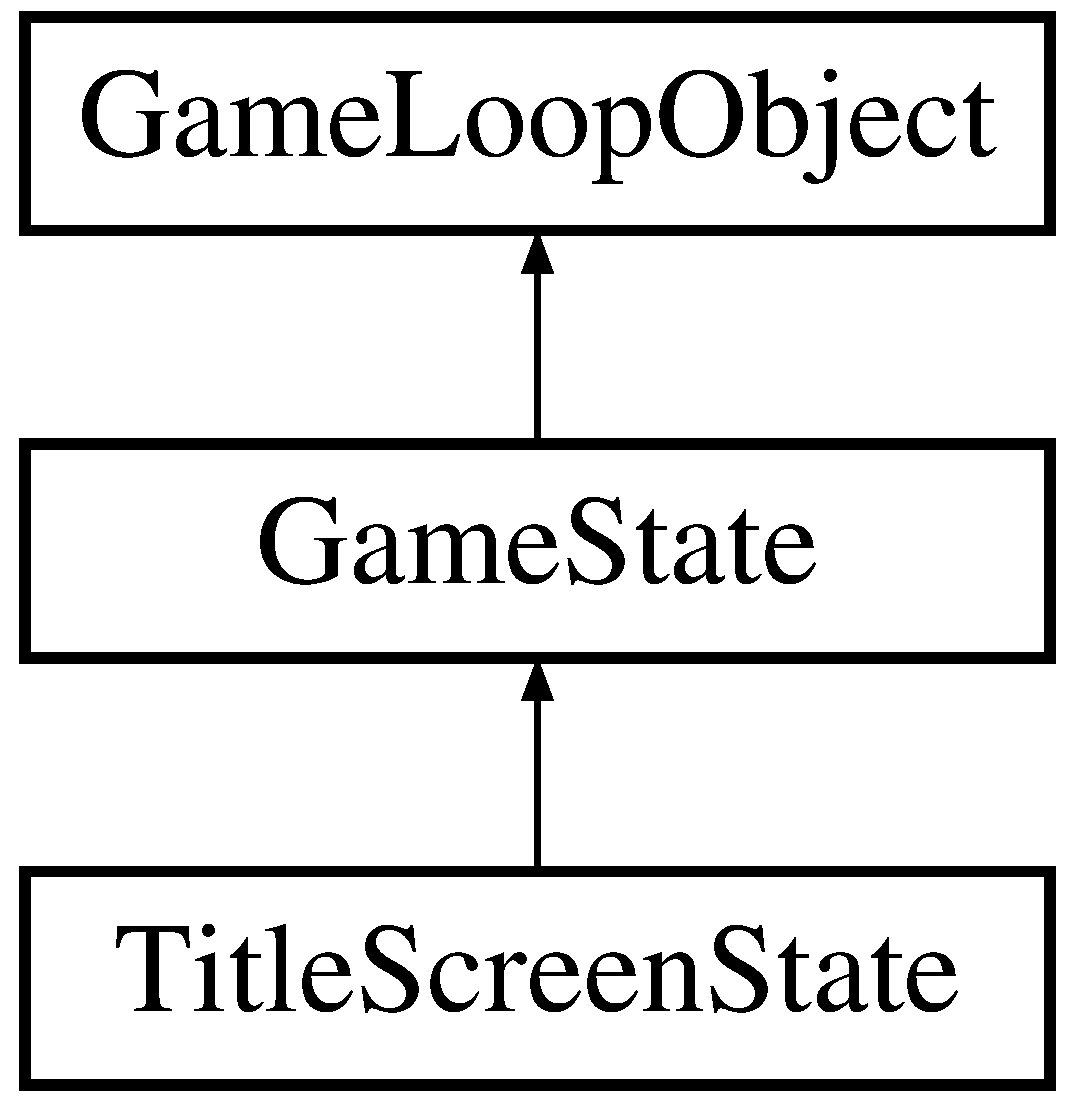
\includegraphics[height=3.000000cm]{class_title_screen_state}
\end{center}
\end{figure}
\subsection*{Public Member Functions}
\begin{DoxyCompactItemize}
\item 
\hyperlink{class_title_screen_state_ae0ab0c01ac47f036618a9d328d547ccd}{Title\+Screen\+State} (sf\+::\+Render\+Window \&window, \hyperlink{class_game_state_manager}{Game\+State\+Manager} \&gsm, \hyperlink{struct_controls_input}{Controls\+Input} \&ci)
\begin{DoxyCompactList}\small\item\em The title screen\textquotesingle{}s constructor method. \end{DoxyCompactList}\item 
void \hyperlink{class_title_screen_state_a1bad900daba7f6481632a58212f39af0}{Handle\+Input} ()
\begin{DoxyCompactList}\small\item\em The title screen\textquotesingle{}s game loop method for handling user input. \end{DoxyCompactList}\item 
void \hyperlink{class_title_screen_state_a0db8d35f9d3013155d2e61939d2a47ea}{Update} ()
\begin{DoxyCompactList}\small\item\em The title screen\textquotesingle{}s game loop method for updating the game. \end{DoxyCompactList}\item 
void \hyperlink{class_title_screen_state_a1e1022947dac4a9b69c6bde57fe52217}{Draw} (sf\+::\+Render\+Window \&window)
\begin{DoxyCompactList}\small\item\em The title screen\textquotesingle{}s game loop method for drawing on the window. \end{DoxyCompactList}\item 
void \hyperlink{class_title_screen_state_a7e6cf3ef5534f42a4ca1e75045a45c71}{Reset} ()
\begin{DoxyCompactList}\small\item\em The title screen\textquotesingle{}s reset method. \end{DoxyCompactList}\end{DoxyCompactItemize}


\subsection{Detailed Description}
The gamestate that shows the title screen. The first thing the player sees. 

This game shows the title screen. Pressing space/enter lets the player proceed to the main menu. This state is the first thing the player sees. 

Definition at line 17 of file Title\+Screen\+State.\+hpp.



\subsection{Constructor \& Destructor Documentation}
\mbox{\Hypertarget{class_title_screen_state_ae0ab0c01ac47f036618a9d328d547ccd}\label{class_title_screen_state_ae0ab0c01ac47f036618a9d328d547ccd}} 
\index{Title\+Screen\+State@{Title\+Screen\+State}!Title\+Screen\+State@{Title\+Screen\+State}}
\index{Title\+Screen\+State@{Title\+Screen\+State}!Title\+Screen\+State@{Title\+Screen\+State}}
\subsubsection{\texorpdfstring{Title\+Screen\+State()}{TitleScreenState()}}
{\footnotesize\ttfamily Title\+Screen\+State\+::\+Title\+Screen\+State (\begin{DoxyParamCaption}\item[{sf\+::\+Render\+Window \&}]{window,  }\item[{\hyperlink{class_game_state_manager}{Game\+State\+Manager} \&}]{gsm,  }\item[{\hyperlink{struct_controls_input}{Controls\+Input} \&}]{ci }\end{DoxyParamCaption})}



The title screen\textquotesingle{}s constructor method. 

The title screen\textquotesingle{}s constructor requires the gamestatemanager to be able to switch states and the controlsinput object to read user input. 

Definition at line 5 of file Title\+Screen\+State.\+cpp.



\subsection{Member Function Documentation}
\mbox{\Hypertarget{class_title_screen_state_a1e1022947dac4a9b69c6bde57fe52217}\label{class_title_screen_state_a1e1022947dac4a9b69c6bde57fe52217}} 
\index{Title\+Screen\+State@{Title\+Screen\+State}!Draw@{Draw}}
\index{Draw@{Draw}!Title\+Screen\+State@{Title\+Screen\+State}}
\subsubsection{\texorpdfstring{Draw()}{Draw()}}
{\footnotesize\ttfamily void Title\+Screen\+State\+::\+Draw (\begin{DoxyParamCaption}\item[{sf\+::\+Render\+Window \&}]{window }\end{DoxyParamCaption})\hspace{0.3cm}{\ttfamily [virtual]}}



The title screen\textquotesingle{}s game loop method for drawing on the window. 

Draws the background and text on the screen. Text disappears when the player presses space/enter to proceed to the main menu. 

Reimplemented from \hyperlink{class_game_state_a8741c5c696c6c366beb4b845c08c3cf8}{Game\+State}.



Definition at line 49 of file Title\+Screen\+State.\+cpp.

\mbox{\Hypertarget{class_title_screen_state_a1bad900daba7f6481632a58212f39af0}\label{class_title_screen_state_a1bad900daba7f6481632a58212f39af0}} 
\index{Title\+Screen\+State@{Title\+Screen\+State}!Handle\+Input@{Handle\+Input}}
\index{Handle\+Input@{Handle\+Input}!Title\+Screen\+State@{Title\+Screen\+State}}
\subsubsection{\texorpdfstring{Handle\+Input()}{HandleInput()}}
{\footnotesize\ttfamily void Title\+Screen\+State\+::\+Handle\+Input (\begin{DoxyParamCaption}{ }\end{DoxyParamCaption})\hspace{0.3cm}{\ttfamily [virtual]}}



The title screen\textquotesingle{}s game loop method for handling user input. 

This method handles all user input related to this gamestate. Pressing space/enter lets the player proceed to the main menu. 

Reimplemented from \hyperlink{class_game_state_a8bce2828cee99ae7c07322804531fd01}{Game\+State}.



Definition at line 29 of file Title\+Screen\+State.\+cpp.

\mbox{\Hypertarget{class_title_screen_state_a7e6cf3ef5534f42a4ca1e75045a45c71}\label{class_title_screen_state_a7e6cf3ef5534f42a4ca1e75045a45c71}} 
\index{Title\+Screen\+State@{Title\+Screen\+State}!Reset@{Reset}}
\index{Reset@{Reset}!Title\+Screen\+State@{Title\+Screen\+State}}
\subsubsection{\texorpdfstring{Reset()}{Reset()}}
{\footnotesize\ttfamily void Title\+Screen\+State\+::\+Reset (\begin{DoxyParamCaption}{ }\end{DoxyParamCaption})\hspace{0.3cm}{\ttfamily [virtual]}}



The title screen\textquotesingle{}s reset method. 

Does nothing. 

Reimplemented from \hyperlink{class_game_state_a46ac6317883dff0eba4f8f305af6b6bb}{Game\+State}.



Definition at line 59 of file Title\+Screen\+State.\+cpp.

\mbox{\Hypertarget{class_title_screen_state_a0db8d35f9d3013155d2e61939d2a47ea}\label{class_title_screen_state_a0db8d35f9d3013155d2e61939d2a47ea}} 
\index{Title\+Screen\+State@{Title\+Screen\+State}!Update@{Update}}
\index{Update@{Update}!Title\+Screen\+State@{Title\+Screen\+State}}
\subsubsection{\texorpdfstring{Update()}{Update()}}
{\footnotesize\ttfamily void Title\+Screen\+State\+::\+Update (\begin{DoxyParamCaption}{ }\end{DoxyParamCaption})\hspace{0.3cm}{\ttfamily [virtual]}}



The title screen\textquotesingle{}s game loop method for updating the game. 

Only checks if a gamestate switch should be executed. 

Reimplemented from \hyperlink{class_game_state_a5be51b634f95bc6e57066ad6931aa18b}{Game\+State}.



Definition at line 44 of file Title\+Screen\+State.\+cpp.



The documentation for this class was generated from the following files\+:\begin{DoxyCompactItemize}
\item 
C\+:/\+Users/joost/\+Documents/\+Git\+Hub/topdown/\+Code/\+Team\+Topdown/\+Team\+Topdown/\hyperlink{_title_screen_state_8hpp}{Title\+Screen\+State.\+hpp}\item 
C\+:/\+Users/joost/\+Documents/\+Git\+Hub/topdown/\+Code/\+Team\+Topdown/\+Team\+Topdown/\hyperlink{_title_screen_state_8cpp}{Title\+Screen\+State.\+cpp}\end{DoxyCompactItemize}

\hypertarget{class_turret}{}\section{Turret Class Reference}
\label{class_turret}\index{Turret@{Turret}}


\hyperlink{class_turret}{Turret} that shoots bullets in a certain direction. This turret is created with a direction in our map, as well as the amount of frames between each shot. The bullets themselves are shot from EC, with the shot timer being contained inside this class. The turret sets a public boolean to true when it is time to shoot and sets it to false. This way, EC can read out the boolean to shoot a bullet.  




{\ttfamily \#include $<$Turret.\+h$>$}

Inheritance diagram for Turret\+:\begin{figure}[H]
\begin{center}
\leavevmode
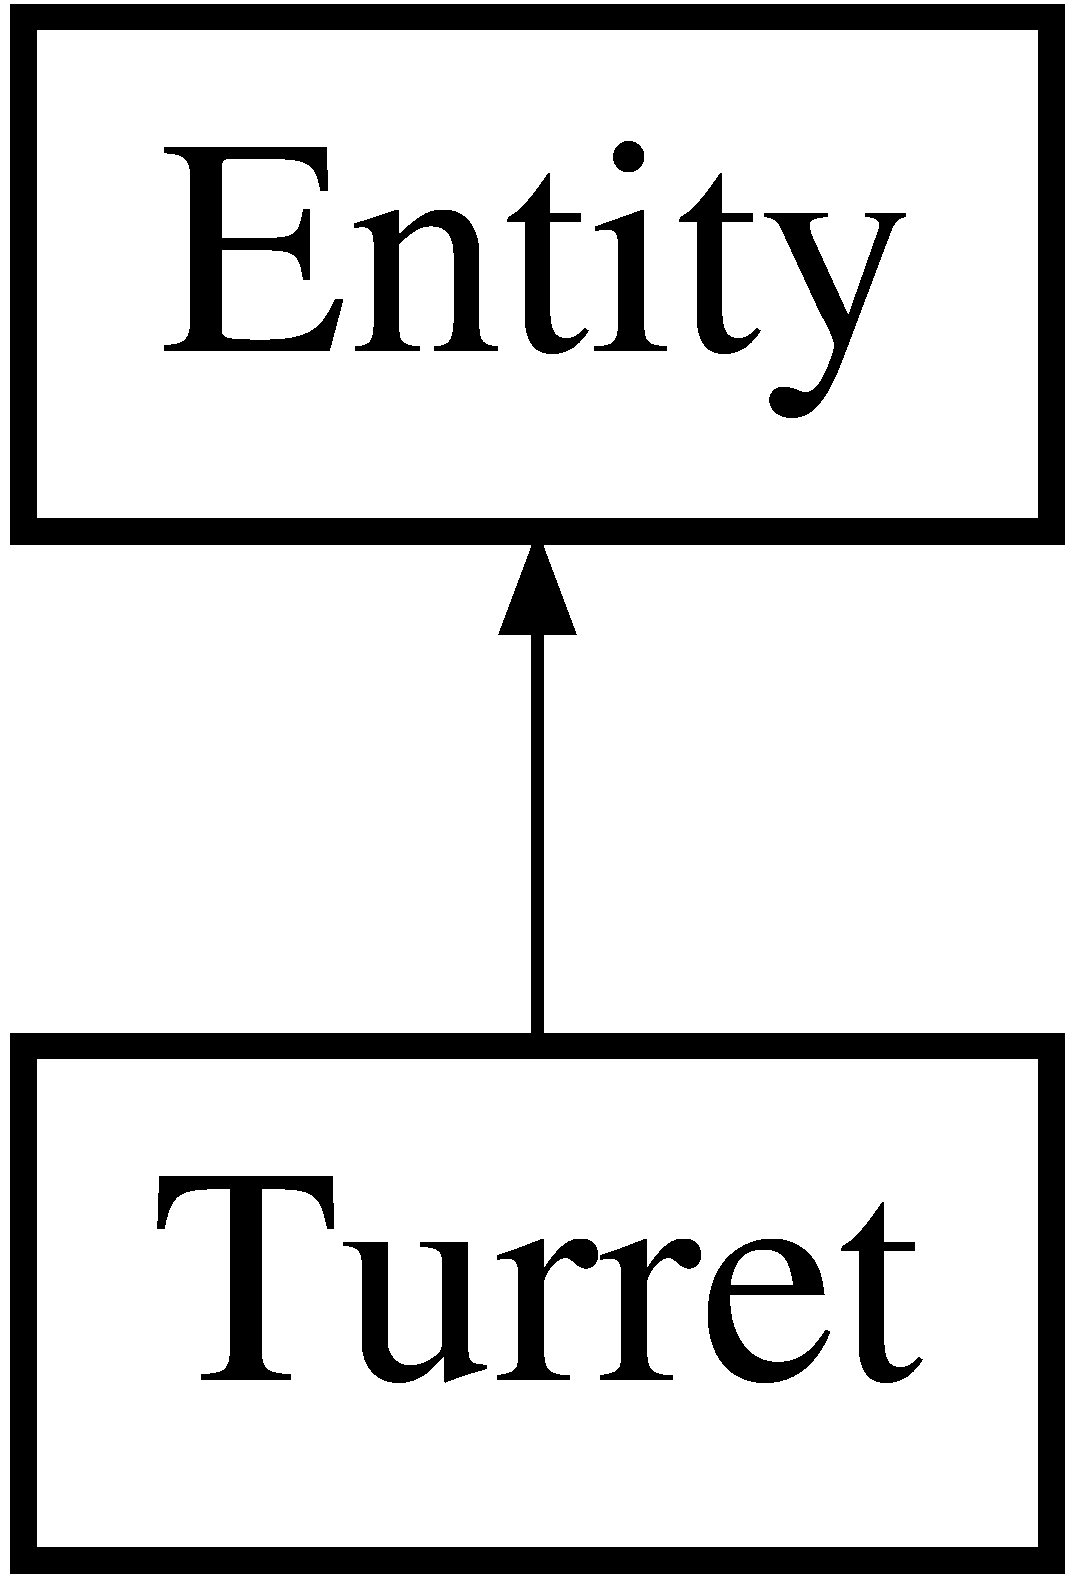
\includegraphics[height=2.000000cm]{class_turret}
\end{center}
\end{figure}
\subsection*{Public Member Functions}
\begin{DoxyCompactItemize}
\item 
\hyperlink{class_turret_a78913e2baf94c133ca9e1e18bcc24304}{Turret} (Vector2f \hyperlink{class_entity_a6af9d6498134ad0906011778bc5736db}{position}, Vector2f \hyperlink{class_entity_ae9a0a364c85f91ade5088b3610131417}{size}, Vector2f look\+At\+Object, int frames\+Between\+Shots=60, bool \hyperlink{class_entity_af1b0754c9d5f4afa73834b23c6437101}{is\+Solid}=true)
\item 
Vector2f \hyperlink{class_turret_aee3e22c1794e60cd8f89d1da39a6e443}{get\+Direction} ()
\item 
Vector2f \hyperlink{class_turret_a706e5a6001c3a0213b7510d4b99c0768}{get\+Pos} () override
\item 
void \hyperlink{class_turret_aad95afd1118f42d424465c14ebb445c7}{update} () override
\item 
\hyperlink{class_entity}{Entity} $\ast$ \hyperlink{class_turret_a141f76a3821b1d08a5aec057506c86e7}{hit} () override
\item 
void \hyperlink{class_turret_a7beef22798d993d9991bd22417034f49}{draw} (Render\+Window \&window) override
\item 
bool \hyperlink{class_turret_ada3f7ae7cdc24a5c24be131beb9887e8}{collides\+With} (\hyperlink{class_entity}{Entity} $\ast$other)
\end{DoxyCompactItemize}
\subsection*{Public Attributes}
\begin{DoxyCompactItemize}
\item 
bool \hyperlink{class_turret_a342932889ec85dbc05e73341ad658e19}{will\+Shoot} = false
\end{DoxyCompactItemize}
\subsection*{Additional Inherited Members}


\subsection{Detailed Description}
\hyperlink{class_turret}{Turret} that shoots bullets in a certain direction. This turret is created with a direction in our map, as well as the amount of frames between each shot. The bullets themselves are shot from EC, with the shot timer being contained inside this class. The turret sets a public boolean to true when it is time to shoot and sets it to false. This way, EC can read out the boolean to shoot a bullet. 

Definition at line 13 of file Turret.\+h.



\subsection{Constructor \& Destructor Documentation}
\mbox{\Hypertarget{class_turret_a78913e2baf94c133ca9e1e18bcc24304}\label{class_turret_a78913e2baf94c133ca9e1e18bcc24304}} 
\index{Turret@{Turret}!Turret@{Turret}}
\index{Turret@{Turret}!Turret@{Turret}}
\subsubsection{\texorpdfstring{Turret()}{Turret()}}
{\footnotesize\ttfamily Turret\+::\+Turret (\begin{DoxyParamCaption}\item[{Vector2f}]{position,  }\item[{Vector2f}]{size,  }\item[{Vector2f}]{look\+At\+Object,  }\item[{int}]{frames\+Between\+Shots = {\ttfamily 60},  }\item[{bool}]{is\+Solid = {\ttfamily true} }\end{DoxyParamCaption})}



Definition at line 5 of file Turret.\+cpp.



\subsection{Member Function Documentation}
\mbox{\Hypertarget{class_turret_ada3f7ae7cdc24a5c24be131beb9887e8}\label{class_turret_ada3f7ae7cdc24a5c24be131beb9887e8}} 
\index{Turret@{Turret}!collides\+With@{collides\+With}}
\index{collides\+With@{collides\+With}!Turret@{Turret}}
\subsubsection{\texorpdfstring{collides\+With()}{collidesWith()}}
{\footnotesize\ttfamily bool Turret\+::collides\+With (\begin{DoxyParamCaption}\item[{\hyperlink{class_entity}{Entity} $\ast$}]{other }\end{DoxyParamCaption})}



Definition at line 54 of file Turret.\+cpp.

\mbox{\Hypertarget{class_turret_a7beef22798d993d9991bd22417034f49}\label{class_turret_a7beef22798d993d9991bd22417034f49}} 
\index{Turret@{Turret}!draw@{draw}}
\index{draw@{draw}!Turret@{Turret}}
\subsubsection{\texorpdfstring{draw()}{draw()}}
{\footnotesize\ttfamily void Turret\+::draw (\begin{DoxyParamCaption}\item[{Render\+Window \&}]{window }\end{DoxyParamCaption})\hspace{0.3cm}{\ttfamily [override]}, {\ttfamily [virtual]}}



Reimplemented from \hyperlink{class_entity_a030c3aa6641df7981a2d8a3fba890ec7}{Entity}.



Definition at line 49 of file Turret.\+cpp.

\mbox{\Hypertarget{class_turret_aee3e22c1794e60cd8f89d1da39a6e443}\label{class_turret_aee3e22c1794e60cd8f89d1da39a6e443}} 
\index{Turret@{Turret}!get\+Direction@{get\+Direction}}
\index{get\+Direction@{get\+Direction}!Turret@{Turret}}
\subsubsection{\texorpdfstring{get\+Direction()}{getDirection()}}
{\footnotesize\ttfamily Vector2f Turret\+::get\+Direction (\begin{DoxyParamCaption}{ }\end{DoxyParamCaption})}



Definition at line 20 of file Turret.\+cpp.

\mbox{\Hypertarget{class_turret_a706e5a6001c3a0213b7510d4b99c0768}\label{class_turret_a706e5a6001c3a0213b7510d4b99c0768}} 
\index{Turret@{Turret}!get\+Pos@{get\+Pos}}
\index{get\+Pos@{get\+Pos}!Turret@{Turret}}
\subsubsection{\texorpdfstring{get\+Pos()}{getPos()}}
{\footnotesize\ttfamily Vector2f Turret\+::get\+Pos (\begin{DoxyParamCaption}{ }\end{DoxyParamCaption})\hspace{0.3cm}{\ttfamily [override]}, {\ttfamily [virtual]}}



Reimplemented from \hyperlink{class_entity_a8b6080f0ab76702fcd00108aef8ea9dd}{Entity}.



Definition at line 24 of file Turret.\+cpp.

\mbox{\Hypertarget{class_turret_a141f76a3821b1d08a5aec057506c86e7}\label{class_turret_a141f76a3821b1d08a5aec057506c86e7}} 
\index{Turret@{Turret}!hit@{hit}}
\index{hit@{hit}!Turret@{Turret}}
\subsubsection{\texorpdfstring{hit()}{hit()}}
{\footnotesize\ttfamily \hyperlink{class_entity}{Entity} $\ast$ Turret\+::hit (\begin{DoxyParamCaption}{ }\end{DoxyParamCaption})\hspace{0.3cm}{\ttfamily [override]}, {\ttfamily [virtual]}}



Reimplemented from \hyperlink{class_entity_a29117f3f40e7069d5d4c1b2fca7819d6}{Entity}.



Definition at line 41 of file Turret.\+cpp.

\mbox{\Hypertarget{class_turret_aad95afd1118f42d424465c14ebb445c7}\label{class_turret_aad95afd1118f42d424465c14ebb445c7}} 
\index{Turret@{Turret}!update@{update}}
\index{update@{update}!Turret@{Turret}}
\subsubsection{\texorpdfstring{update()}{update()}}
{\footnotesize\ttfamily void Turret\+::update (\begin{DoxyParamCaption}{ }\end{DoxyParamCaption})\hspace{0.3cm}{\ttfamily [override]}, {\ttfamily [virtual]}}



Reimplemented from \hyperlink{class_entity_aed73e98b980b85833428c935cc1c69f8}{Entity}.



Definition at line 28 of file Turret.\+cpp.



\subsection{Member Data Documentation}
\mbox{\Hypertarget{class_turret_a342932889ec85dbc05e73341ad658e19}\label{class_turret_a342932889ec85dbc05e73341ad658e19}} 
\index{Turret@{Turret}!will\+Shoot@{will\+Shoot}}
\index{will\+Shoot@{will\+Shoot}!Turret@{Turret}}
\subsubsection{\texorpdfstring{will\+Shoot}{willShoot}}
{\footnotesize\ttfamily bool Turret\+::will\+Shoot = false}



Definition at line 23 of file Turret.\+h.



The documentation for this class was generated from the following files\+:\begin{DoxyCompactItemize}
\item 
C\+:/\+Users/joost/\+Documents/\+Git\+Hub/topdown/\+Code/\+Team\+Topdown/\+Team\+Topdown/\hyperlink{_turret_8h}{Turret.\+h}\item 
C\+:/\+Users/joost/\+Documents/\+Git\+Hub/topdown/\+Code/\+Team\+Topdown/\+Team\+Topdown/\hyperlink{_turret_8cpp}{Turret.\+cpp}\end{DoxyCompactItemize}

\hypertarget{classvision_bullet}{}\section{vision\+Bullet Class Reference}
\label{classvision_bullet}\index{vision\+Bullet@{vision\+Bullet}}


Invisible bullets to detect enemy vision.  




{\ttfamily \#include $<$vision\+Bullet.\+h$>$}

Inheritance diagram for vision\+Bullet\+:\begin{figure}[H]
\begin{center}
\leavevmode
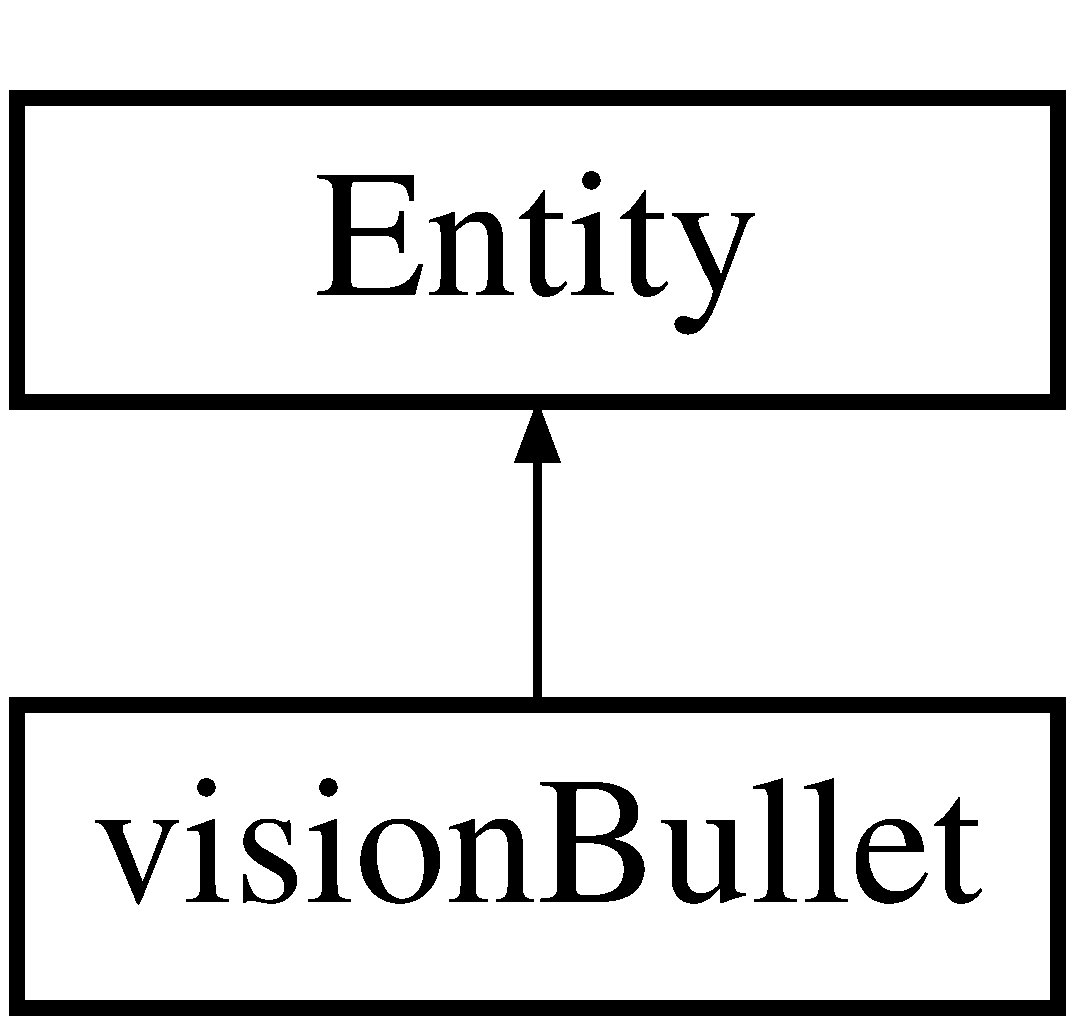
\includegraphics[height=2.000000cm]{classvision_bullet}
\end{center}
\end{figure}
\subsection*{Public Member Functions}
\begin{DoxyCompactItemize}
\item 
\hyperlink{classvision_bullet_af168dc7280da3a5663fc7d91518ff005}{vision\+Bullet} (float speed, Vector2f relative\+Pos\+Bul, Vector2f \hyperlink{class_entity_a6af9d6498134ad0906011778bc5736db}{position}, Vector2f \hyperlink{class_entity_ae9a0a364c85f91ade5088b3610131417}{size}, bool \hyperlink{class_entity_af1b0754c9d5f4afa73834b23c6437101}{is\+Solid}=true, int \hyperlink{class_entity_a4edd9cc2506add0d9e27fade0bf957e8}{state}=2)
\item 
\hyperlink{classvision_bullet_aa96d05163bb81ae5c86f173cbd36de3b}{$\sim$vision\+Bullet} ()
\item 
bool \hyperlink{classvision_bullet_a01a4cf06a2403aa6dce98ecd52b23bf0}{get\+Is\+Alive} ()
\item 
void \hyperlink{classvision_bullet_a67881b6eb8c31e128ff1ecc5ed110855}{set\+Is\+Alive} (bool b)
\item 
Vector2f \hyperlink{classvision_bullet_a381783842104058048b9abffb693d55e}{get\+Direction} ()
\item 
void \hyperlink{classvision_bullet_a425ac17ace4a29879a9a204ffc29021d}{update} ()
\item 
void \hyperlink{classvision_bullet_ab2f4d4a63991b39480e3064ed5ee3809}{draw} (Render\+Window \&window)
\item 
int \hyperlink{classvision_bullet_a152e9b57ee511a97c9050dbf8ed84b90}{get\+Time\+Alive} ()
\end{DoxyCompactItemize}
\subsection*{Additional Inherited Members}


\subsection{Detailed Description}
Invisible bullets to detect enemy vision. 

Definition at line 12 of file vision\+Bullet.\+h.



\subsection{Constructor \& Destructor Documentation}
\mbox{\Hypertarget{classvision_bullet_af168dc7280da3a5663fc7d91518ff005}\label{classvision_bullet_af168dc7280da3a5663fc7d91518ff005}} 
\index{vision\+Bullet@{vision\+Bullet}!vision\+Bullet@{vision\+Bullet}}
\index{vision\+Bullet@{vision\+Bullet}!vision\+Bullet@{vision\+Bullet}}
\subsubsection{\texorpdfstring{vision\+Bullet()}{visionBullet()}}
{\footnotesize\ttfamily vision\+Bullet\+::vision\+Bullet (\begin{DoxyParamCaption}\item[{float}]{speed,  }\item[{Vector2f}]{relative\+Pos\+Bul,  }\item[{Vector2f}]{position,  }\item[{Vector2f}]{size,  }\item[{bool}]{is\+Solid = {\ttfamily true},  }\item[{int}]{state = {\ttfamily 2} }\end{DoxyParamCaption})}

float speed speed in pixels Vector2f relative\+Pos\+Bul the vector with the spawn point as zero point to set the direction Vector2f position the spawn point Vector2f size size of bullet bool is\+Solid 

Definition at line 5 of file vision\+Bullet.\+cpp.

\mbox{\Hypertarget{classvision_bullet_aa96d05163bb81ae5c86f173cbd36de3b}\label{classvision_bullet_aa96d05163bb81ae5c86f173cbd36de3b}} 
\index{vision\+Bullet@{vision\+Bullet}!````~vision\+Bullet@{$\sim$vision\+Bullet}}
\index{````~vision\+Bullet@{$\sim$vision\+Bullet}!vision\+Bullet@{vision\+Bullet}}
\subsubsection{\texorpdfstring{$\sim$vision\+Bullet()}{~visionBullet()}}
{\footnotesize\ttfamily vision\+Bullet\+::$\sim$vision\+Bullet (\begin{DoxyParamCaption}{ }\end{DoxyParamCaption})}



Definition at line 13 of file vision\+Bullet.\+cpp.



\subsection{Member Function Documentation}
\mbox{\Hypertarget{classvision_bullet_ab2f4d4a63991b39480e3064ed5ee3809}\label{classvision_bullet_ab2f4d4a63991b39480e3064ed5ee3809}} 
\index{vision\+Bullet@{vision\+Bullet}!draw@{draw}}
\index{draw@{draw}!vision\+Bullet@{vision\+Bullet}}
\subsubsection{\texorpdfstring{draw()}{draw()}}
{\footnotesize\ttfamily void vision\+Bullet\+::draw (\begin{DoxyParamCaption}\item[{Render\+Window \&}]{window }\end{DoxyParamCaption})\hspace{0.3cm}{\ttfamily [virtual]}}

draw the bullet Render\+Window window window to draw in 

Reimplemented from \hyperlink{class_entity_a030c3aa6641df7981a2d8a3fba890ec7}{Entity}.



Definition at line 43 of file vision\+Bullet.\+cpp.

\mbox{\Hypertarget{classvision_bullet_a381783842104058048b9abffb693d55e}\label{classvision_bullet_a381783842104058048b9abffb693d55e}} 
\index{vision\+Bullet@{vision\+Bullet}!get\+Direction@{get\+Direction}}
\index{get\+Direction@{get\+Direction}!vision\+Bullet@{vision\+Bullet}}
\subsubsection{\texorpdfstring{get\+Direction()}{getDirection()}}
{\footnotesize\ttfamily Vector2f vision\+Bullet\+::get\+Direction (\begin{DoxyParamCaption}{ }\end{DoxyParamCaption})}

get the direction where the bullet will be after the next update 

Definition at line 35 of file vision\+Bullet.\+cpp.

\mbox{\Hypertarget{classvision_bullet_a01a4cf06a2403aa6dce98ecd52b23bf0}\label{classvision_bullet_a01a4cf06a2403aa6dce98ecd52b23bf0}} 
\index{vision\+Bullet@{vision\+Bullet}!get\+Is\+Alive@{get\+Is\+Alive}}
\index{get\+Is\+Alive@{get\+Is\+Alive}!vision\+Bullet@{vision\+Bullet}}
\subsubsection{\texorpdfstring{get\+Is\+Alive()}{getIsAlive()}}
{\footnotesize\ttfamily bool vision\+Bullet\+::get\+Is\+Alive (\begin{DoxyParamCaption}{ }\end{DoxyParamCaption})}

getter to know if bullet still is active 

Definition at line 31 of file vision\+Bullet.\+cpp.

\mbox{\Hypertarget{classvision_bullet_a152e9b57ee511a97c9050dbf8ed84b90}\label{classvision_bullet_a152e9b57ee511a97c9050dbf8ed84b90}} 
\index{vision\+Bullet@{vision\+Bullet}!get\+Time\+Alive@{get\+Time\+Alive}}
\index{get\+Time\+Alive@{get\+Time\+Alive}!vision\+Bullet@{vision\+Bullet}}
\subsubsection{\texorpdfstring{get\+Time\+Alive()}{getTimeAlive()}}
{\footnotesize\ttfamily int vision\+Bullet\+::get\+Time\+Alive (\begin{DoxyParamCaption}{ }\end{DoxyParamCaption})}

\textbackslash{} details get the time the bullet is active 

Definition at line 39 of file vision\+Bullet.\+cpp.

\mbox{\Hypertarget{classvision_bullet_a67881b6eb8c31e128ff1ecc5ed110855}\label{classvision_bullet_a67881b6eb8c31e128ff1ecc5ed110855}} 
\index{vision\+Bullet@{vision\+Bullet}!set\+Is\+Alive@{set\+Is\+Alive}}
\index{set\+Is\+Alive@{set\+Is\+Alive}!vision\+Bullet@{vision\+Bullet}}
\subsubsection{\texorpdfstring{set\+Is\+Alive()}{setIsAlive()}}
{\footnotesize\ttfamily void vision\+Bullet\+::set\+Is\+Alive (\begin{DoxyParamCaption}\item[{bool}]{b }\end{DoxyParamCaption})}

setter to set bullet active or inactive 

Definition at line 27 of file vision\+Bullet.\+cpp.

\mbox{\Hypertarget{classvision_bullet_a425ac17ace4a29879a9a204ffc29021d}\label{classvision_bullet_a425ac17ace4a29879a9a204ffc29021d}} 
\index{vision\+Bullet@{vision\+Bullet}!update@{update}}
\index{update@{update}!vision\+Bullet@{vision\+Bullet}}
\subsubsection{\texorpdfstring{update()}{update()}}
{\footnotesize\ttfamily void vision\+Bullet\+::update (\begin{DoxyParamCaption}{ }\end{DoxyParamCaption})\hspace{0.3cm}{\ttfamily [virtual]}}

update the position of the bullet 

Reimplemented from \hyperlink{class_entity_aed73e98b980b85833428c935cc1c69f8}{Entity}.



Definition at line 16 of file vision\+Bullet.\+cpp.



The documentation for this class was generated from the following files\+:\begin{DoxyCompactItemize}
\item 
C\+:/\+Users/joost/\+Documents/\+Git\+Hub/topdown/\+Code/\+Team\+Topdown/\+Team\+Topdown/\hyperlink{vision_bullet_8h}{vision\+Bullet.\+h}\item 
C\+:/\+Users/joost/\+Documents/\+Git\+Hub/topdown/\+Code/\+Team\+Topdown/\+Team\+Topdown/\hyperlink{vision_bullet_8cpp}{vision\+Bullet.\+cpp}\end{DoxyCompactItemize}

\hypertarget{class_wall}{}\section{Wall Class Reference}
\label{class_wall}\index{Wall@{Wall}}


(invisible) \hyperlink{class_wall}{Wall} class This class represents an invisible wall-\/tile. Its position is a multitude of (32,32) and its size is exactly (32,32). It cannot update, since our position is always set, and it cannot draw, because it is invisible. So we override those functions with empty brackets.  




{\ttfamily \#include $<$Wall.\+h$>$}

Inheritance diagram for Wall\+:\begin{figure}[H]
\begin{center}
\leavevmode
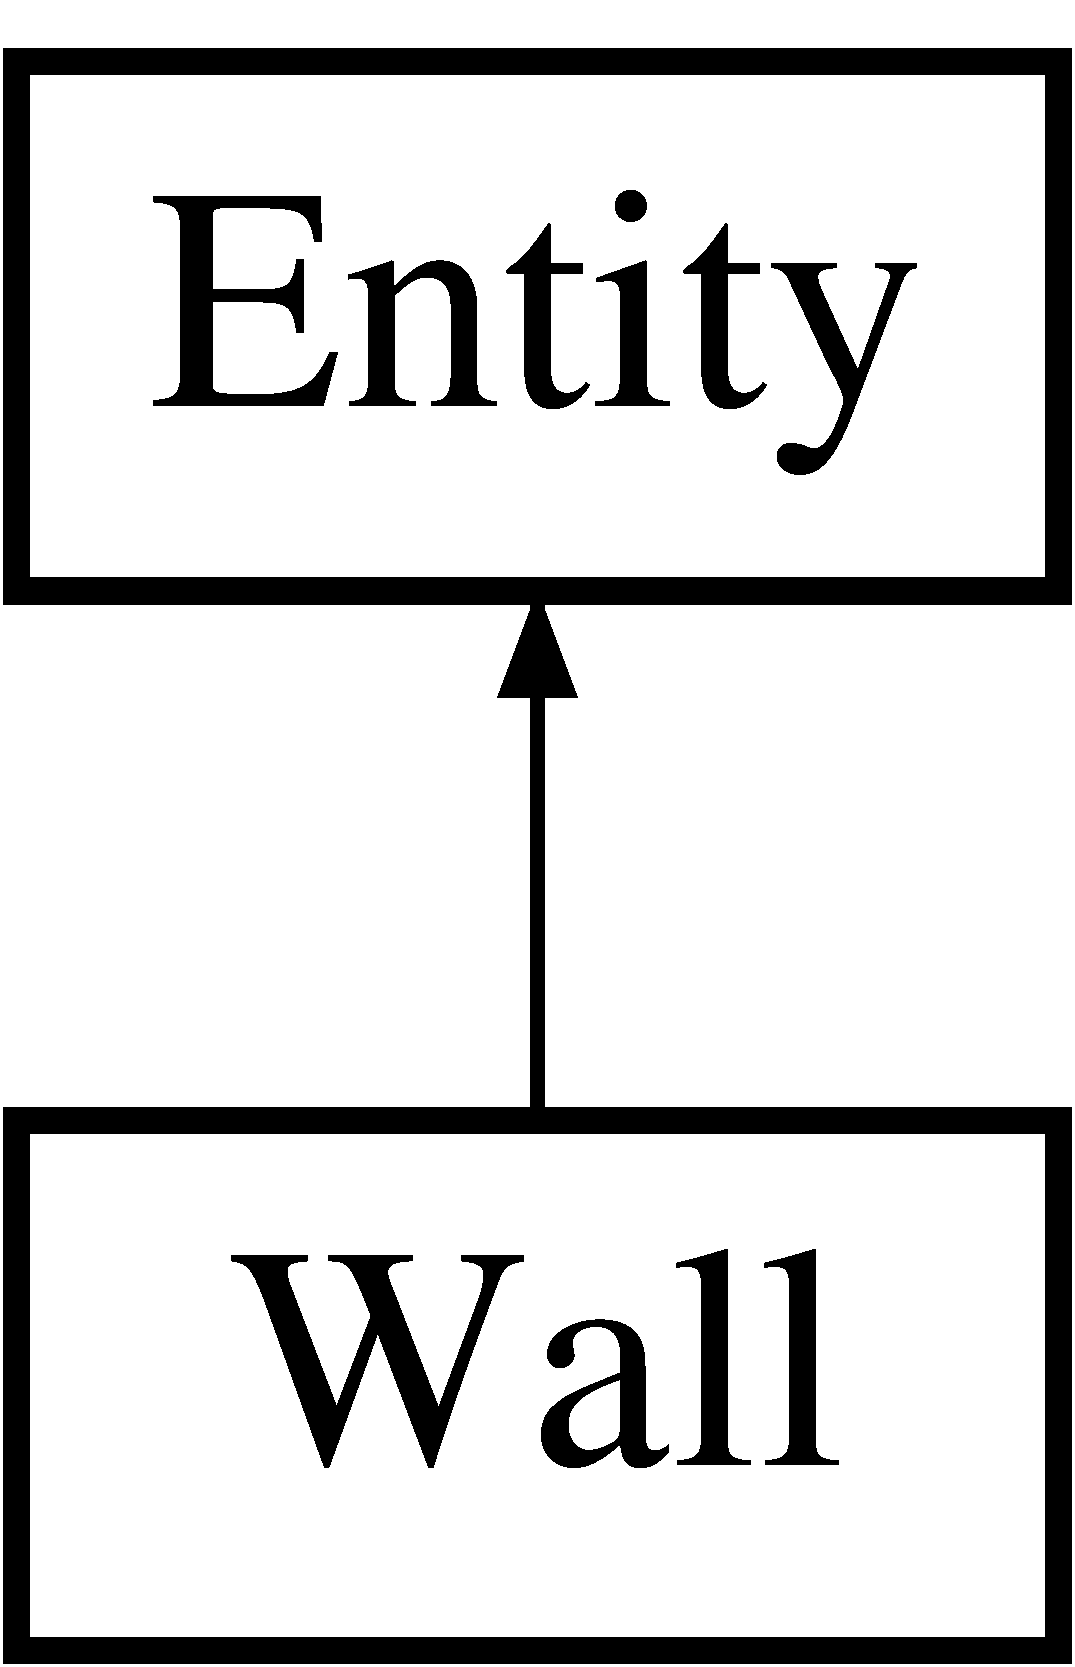
\includegraphics[height=2.000000cm]{class_wall}
\end{center}
\end{figure}
\subsection*{Public Member Functions}
\begin{DoxyCompactItemize}
\item 
\hyperlink{class_wall_ad8db4b51570f4a83de3750082f826516}{Wall} (Vector2f \hyperlink{class_entity_a6af9d6498134ad0906011778bc5736db}{position}, Vector2f \hyperlink{class_entity_ae9a0a364c85f91ade5088b3610131417}{size})
\end{DoxyCompactItemize}
\subsection*{Additional Inherited Members}


\subsection{Detailed Description}
(invisible) \hyperlink{class_wall}{Wall} class This class represents an invisible wall-\/tile. Its position is a multitude of (32,32) and its size is exactly (32,32). It cannot update, since our position is always set, and it cannot draw, because it is invisible. So we override those functions with empty brackets. 

Definition at line 13 of file Wall.\+h.



\subsection{Constructor \& Destructor Documentation}
\mbox{\Hypertarget{class_wall_ad8db4b51570f4a83de3750082f826516}\label{class_wall_ad8db4b51570f4a83de3750082f826516}} 
\index{Wall@{Wall}!Wall@{Wall}}
\index{Wall@{Wall}!Wall@{Wall}}
\subsubsection{\texorpdfstring{Wall()}{Wall()}}
{\footnotesize\ttfamily Wall\+::\+Wall (\begin{DoxyParamCaption}\item[{Vector2f}]{position,  }\item[{Vector2f}]{size }\end{DoxyParamCaption})}



Definition at line 5 of file Wall.\+cpp.



The documentation for this class was generated from the following files\+:\begin{DoxyCompactItemize}
\item 
C\+:/\+Users/joost/\+Documents/\+Git\+Hub/topdown/\+Code/\+Team\+Topdown/\+Team\+Topdown/\hyperlink{_wall_8h}{Wall.\+h}\item 
C\+:/\+Users/joost/\+Documents/\+Git\+Hub/topdown/\+Code/\+Team\+Topdown/\+Team\+Topdown/\hyperlink{_wall_8cpp}{Wall.\+cpp}\end{DoxyCompactItemize}

\chapter{File Documentation}
\hypertarget{_all_game_states_8hpp}{}\section{C\+:/\+Users/joost/\+Documents/\+Git\+Hub/topdown/\+Code/\+Team\+Topdown/\+Team\+Topdown/\+All\+Game\+States.hpp File Reference}
\label{_all_game_states_8hpp}\index{C\+:/\+Users/joost/\+Documents/\+Git\+Hub/topdown/\+Code/\+Team\+Topdown/\+Team\+Topdown/\+All\+Game\+States.\+hpp@{C\+:/\+Users/joost/\+Documents/\+Git\+Hub/topdown/\+Code/\+Team\+Topdown/\+Team\+Topdown/\+All\+Game\+States.\+hpp}}
{\ttfamily \#include \char`\"{}Title\+Screen\+State.\+hpp\char`\"{}}\newline
{\ttfamily \#include \char`\"{}Highscores\+State.\+hpp\char`\"{}}\newline
{\ttfamily \#include \char`\"{}Credits\+State.\+hpp\char`\"{}}\newline
{\ttfamily \#include \char`\"{}Main\+Menu\+State.\+hpp\char`\"{}}\newline
{\ttfamily \#include \char`\"{}Playing\+State.\+hpp\char`\"{}}\newline

\hypertarget{bullet_8cpp}{}\section{C\+:/\+Users/joost/\+Documents/\+Git\+Hub/topdown/\+Code/\+Team\+Topdown/\+Team\+Topdown/bullet.cpp File Reference}
\label{bullet_8cpp}\index{C\+:/\+Users/joost/\+Documents/\+Git\+Hub/topdown/\+Code/\+Team\+Topdown/\+Team\+Topdown/bullet.\+cpp@{C\+:/\+Users/joost/\+Documents/\+Git\+Hub/topdown/\+Code/\+Team\+Topdown/\+Team\+Topdown/bullet.\+cpp}}
{\ttfamily \#include \char`\"{}stdafx.\+h\char`\"{}}\newline
{\ttfamily \#include \char`\"{}bullet.\+h\char`\"{}}\newline

\hypertarget{bullet_8h}{}\section{C\+:/\+Users/joost/\+Documents/\+Git\+Hub/topdown/\+Code/\+Team\+Topdown/\+Team\+Topdown/bullet.h File Reference}
\label{bullet_8h}\index{C\+:/\+Users/joost/\+Documents/\+Git\+Hub/topdown/\+Code/\+Team\+Topdown/\+Team\+Topdown/bullet.\+h@{C\+:/\+Users/joost/\+Documents/\+Git\+Hub/topdown/\+Code/\+Team\+Topdown/\+Team\+Topdown/bullet.\+h}}
{\ttfamily \#include \char`\"{}stdafx.\+h\char`\"{}}\newline
{\ttfamily \#include $<$iostream$>$}\newline
{\ttfamily \#include $<$windows.\+h$>$}\newline
{\ttfamily \#include \char`\"{}Entity.\+h\char`\"{}}\newline
{\ttfamily \#include \char`\"{}Graphic.\+h\char`\"{}}\newline
{\ttfamily \#include $<$S\+F\+M\+L/\+Graphics.\+hpp$>$}\newline
\subsection*{Classes}
\begin{DoxyCompactItemize}
\item 
class \hyperlink{class_bullet}{Bullet}
\begin{DoxyCompactList}\small\item\em A bullet object is an entity that`s always moving in one direction. \end{DoxyCompactList}\end{DoxyCompactItemize}

\hypertarget{_camera_8cpp}{}\section{C\+:/\+Users/joost/\+Documents/\+Git\+Hub/topdown/\+Code/\+Team\+Topdown/\+Team\+Topdown/\+Camera.cpp File Reference}
\label{_camera_8cpp}\index{C\+:/\+Users/joost/\+Documents/\+Git\+Hub/topdown/\+Code/\+Team\+Topdown/\+Team\+Topdown/\+Camera.\+cpp@{C\+:/\+Users/joost/\+Documents/\+Git\+Hub/topdown/\+Code/\+Team\+Topdown/\+Team\+Topdown/\+Camera.\+cpp}}
{\ttfamily \#include \char`\"{}stdafx.\+h\char`\"{}}\newline
{\ttfamily \#include \char`\"{}Camera.\+h\char`\"{}}\newline

\hypertarget{_camera_8h}{}\section{C\+:/\+Users/joost/\+Documents/\+Git\+Hub/topdown/\+Code/\+Team\+Topdown/\+Team\+Topdown/\+Camera.h File Reference}
\label{_camera_8h}\index{C\+:/\+Users/joost/\+Documents/\+Git\+Hub/topdown/\+Code/\+Team\+Topdown/\+Team\+Topdown/\+Camera.\+h@{C\+:/\+Users/joost/\+Documents/\+Git\+Hub/topdown/\+Code/\+Team\+Topdown/\+Team\+Topdown/\+Camera.\+h}}
{\ttfamily \#include \char`\"{}stdafx.\+h\char`\"{}}\newline
{\ttfamily \#include $<$iostream$>$}\newline
{\ttfamily \#include $<$windows.\+h$>$}\newline
{\ttfamily \#include \char`\"{}Player.\+h\char`\"{}}\newline
{\ttfamily \#include $<$S\+F\+M\+L/\+Graphics.\+hpp$>$}\newline
{\ttfamily \#include \char`\"{}Timer.\+h\char`\"{}}\newline
\subsection*{Classes}
\begin{DoxyCompactItemize}
\item 
class \hyperlink{class_camera}{Camera}
\end{DoxyCompactItemize}

\hypertarget{_clickable_button_8cpp}{}\section{C\+:/\+Users/joost/\+Documents/\+Git\+Hub/topdown/\+Code/\+Team\+Topdown/\+Team\+Topdown/\+Clickable\+Button.cpp File Reference}
\label{_clickable_button_8cpp}\index{C\+:/\+Users/joost/\+Documents/\+Git\+Hub/topdown/\+Code/\+Team\+Topdown/\+Team\+Topdown/\+Clickable\+Button.\+cpp@{C\+:/\+Users/joost/\+Documents/\+Git\+Hub/topdown/\+Code/\+Team\+Topdown/\+Team\+Topdown/\+Clickable\+Button.\+cpp}}
{\ttfamily \#include \char`\"{}stdafx.\+h\char`\"{}}\newline
{\ttfamily \#include \char`\"{}Clickable\+Button.\+hpp\char`\"{}}\newline
{\ttfamily \#include $<$iostream$>$}\newline

\hypertarget{_clickable_button_8hpp}{}\section{C\+:/\+Users/joost/\+Documents/\+Git\+Hub/topdown/\+Code/\+Team\+Topdown/\+Team\+Topdown/\+Clickable\+Button.hpp File Reference}
\label{_clickable_button_8hpp}\index{C\+:/\+Users/joost/\+Documents/\+Git\+Hub/topdown/\+Code/\+Team\+Topdown/\+Team\+Topdown/\+Clickable\+Button.\+hpp@{C\+:/\+Users/joost/\+Documents/\+Git\+Hub/topdown/\+Code/\+Team\+Topdown/\+Team\+Topdown/\+Clickable\+Button.\+hpp}}
{\ttfamily \#include \char`\"{}stdafx.\+h\char`\"{}}\newline
{\ttfamily \#include \char`\"{}Game\+Loop\+Object.\+hpp\char`\"{}}\newline
{\ttfamily \#include \char`\"{}S\+F\+M\+L\textbackslash{}\+Audio.\+hpp\char`\"{}}\newline
\subsection*{Classes}
\begin{DoxyCompactItemize}
\item 
class \hyperlink{class_clickable_button}{Clickable\+Button}
\begin{DoxyCompactList}\small\item\em A clickable button with text, animation and auto-\/resize to text width. \end{DoxyCompactList}\end{DoxyCompactItemize}

\hypertarget{controls_controller_8cpp}{}\section{C\+:/\+Users/joost/\+Documents/\+Git\+Hub/topdown/\+Code/\+Team\+Topdown/\+Team\+Topdown/controls\+Controller.cpp File Reference}
\label{controls_controller_8cpp}\index{C\+:/\+Users/joost/\+Documents/\+Git\+Hub/topdown/\+Code/\+Team\+Topdown/\+Team\+Topdown/controls\+Controller.\+cpp@{C\+:/\+Users/joost/\+Documents/\+Git\+Hub/topdown/\+Code/\+Team\+Topdown/\+Team\+Topdown/controls\+Controller.\+cpp}}
{\ttfamily \#include \char`\"{}stdafx.\+h\char`\"{}}\newline
{\ttfamily \#include \char`\"{}Controls\+Controller.\+h\char`\"{}}\newline

\hypertarget{controls_controller_8h}{}\section{C\+:/\+Users/joost/\+Documents/\+Git\+Hub/topdown/\+Code/\+Team\+Topdown/\+Team\+Topdown/controls\+Controller.h File Reference}
\label{controls_controller_8h}\index{C\+:/\+Users/joost/\+Documents/\+Git\+Hub/topdown/\+Code/\+Team\+Topdown/\+Team\+Topdown/controls\+Controller.\+h@{C\+:/\+Users/joost/\+Documents/\+Git\+Hub/topdown/\+Code/\+Team\+Topdown/\+Team\+Topdown/controls\+Controller.\+h}}
{\ttfamily \#include \char`\"{}stdafx.\+h\char`\"{}}\newline
{\ttfamily \#include $<$iostream$>$}\newline
{\ttfamily \#include $<$windows.\+h$>$}\newline
{\ttfamily \#include \char`\"{}Controls\+Input.\+h\char`\"{}}\newline
{\ttfamily \#include $<$S\+F\+M\+L/\+Graphics.\+hpp$>$}\newline
\subsection*{Classes}
\begin{DoxyCompactItemize}
\item 
class \hyperlink{class_controls_handler}{Controls\+Handler}
\item 
class \hyperlink{class_controls_controller}{Controls\+Controller}
\end{DoxyCompactItemize}

\hypertarget{controls_input_8cpp}{}\section{C\+:/\+Users/joost/\+Documents/\+Git\+Hub/topdown/\+Code/\+Team\+Topdown/\+Team\+Topdown/controls\+Input.cpp File Reference}
\label{controls_input_8cpp}\index{C\+:/\+Users/joost/\+Documents/\+Git\+Hub/topdown/\+Code/\+Team\+Topdown/\+Team\+Topdown/controls\+Input.\+cpp@{C\+:/\+Users/joost/\+Documents/\+Git\+Hub/topdown/\+Code/\+Team\+Topdown/\+Team\+Topdown/controls\+Input.\+cpp}}
{\ttfamily \#include \char`\"{}stdafx.\+h\char`\"{}}\newline
{\ttfamily \#include \char`\"{}Controls\+Input.\+h\char`\"{}}\newline

\hypertarget{controls_input_8h}{}\section{C\+:/\+Users/joost/\+Documents/\+Git\+Hub/topdown/\+Code/\+Team\+Topdown/\+Team\+Topdown/controls\+Input.h File Reference}
\label{controls_input_8h}\index{C\+:/\+Users/joost/\+Documents/\+Git\+Hub/topdown/\+Code/\+Team\+Topdown/\+Team\+Topdown/controls\+Input.\+h@{C\+:/\+Users/joost/\+Documents/\+Git\+Hub/topdown/\+Code/\+Team\+Topdown/\+Team\+Topdown/controls\+Input.\+h}}
{\ttfamily \#include \char`\"{}stdafx.\+h\char`\"{}}\newline
{\ttfamily \#include $<$iostream$>$}\newline
{\ttfamily \#include $<$windows.\+h$>$}\newline
{\ttfamily \#include $<$S\+F\+M\+L/\+Graphics.\+hpp$>$}\newline
\subsection*{Classes}
\begin{DoxyCompactItemize}
\item 
struct \hyperlink{struct_controls_input}{Controls\+Input}
\end{DoxyCompactItemize}

\hypertarget{_crate_8cpp}{}\section{C\+:/\+Users/joost/\+Documents/\+Git\+Hub/topdown/\+Code/\+Team\+Topdown/\+Team\+Topdown/\+Crate.cpp File Reference}
\label{_crate_8cpp}\index{C\+:/\+Users/joost/\+Documents/\+Git\+Hub/topdown/\+Code/\+Team\+Topdown/\+Team\+Topdown/\+Crate.\+cpp@{C\+:/\+Users/joost/\+Documents/\+Git\+Hub/topdown/\+Code/\+Team\+Topdown/\+Team\+Topdown/\+Crate.\+cpp}}
{\ttfamily \#include \char`\"{}stdafx.\+h\char`\"{}}\newline
{\ttfamily \#include \char`\"{}Crate.\+h\char`\"{}}\newline
{\ttfamily \#include $<$cstdlib$>$}\newline

\hypertarget{_crate_8h}{}\section{C\+:/\+Users/joost/\+Documents/\+Git\+Hub/topdown/\+Code/\+Team\+Topdown/\+Team\+Topdown/\+Crate.h File Reference}
\label{_crate_8h}\index{C\+:/\+Users/joost/\+Documents/\+Git\+Hub/topdown/\+Code/\+Team\+Topdown/\+Team\+Topdown/\+Crate.\+h@{C\+:/\+Users/joost/\+Documents/\+Git\+Hub/topdown/\+Code/\+Team\+Topdown/\+Team\+Topdown/\+Crate.\+h}}
{\ttfamily \#include \char`\"{}Entity.\+h\char`\"{}}\newline
{\ttfamily \#include \char`\"{}bullet.\+h\char`\"{}}\newline
{\ttfamily \#include \char`\"{}Graphic.\+h\char`\"{}}\newline
{\ttfamily \#include \char`\"{}S\+F\+M\+L\textbackslash{}\+Audio.\+hpp\char`\"{}}\newline
{\ttfamily \#include \char`\"{}Item.\+h\char`\"{}}\newline
\subsection*{Classes}
\begin{DoxyCompactItemize}
\item 
class \hyperlink{class_crate}{Crate}
\begin{DoxyCompactList}\small\item\em \hyperlink{class_crate}{Crate} class Contains the crate graphic and overrides the necessary functions from \hyperlink{class_entity}{Entity}. \end{DoxyCompactList}\end{DoxyCompactItemize}

\hypertarget{_credits_state_8cpp}{}\section{C\+:/\+Users/joost/\+Documents/\+Git\+Hub/topdown/\+Code/\+Team\+Topdown/\+Team\+Topdown/\+Credits\+State.cpp File Reference}
\label{_credits_state_8cpp}\index{C\+:/\+Users/joost/\+Documents/\+Git\+Hub/topdown/\+Code/\+Team\+Topdown/\+Team\+Topdown/\+Credits\+State.\+cpp@{C\+:/\+Users/joost/\+Documents/\+Git\+Hub/topdown/\+Code/\+Team\+Topdown/\+Team\+Topdown/\+Credits\+State.\+cpp}}
{\ttfamily \#include \char`\"{}stdafx.\+h\char`\"{}}\newline
{\ttfamily \#include \char`\"{}Credits\+State.\+hpp\char`\"{}}\newline
{\ttfamily \#include $<$iostream$>$}\newline

\hypertarget{_credits_state_8hpp}{}\section{C\+:/\+Users/joost/\+Documents/\+Git\+Hub/topdown/\+Code/\+Team\+Topdown/\+Team\+Topdown/\+Credits\+State.hpp File Reference}
\label{_credits_state_8hpp}\index{C\+:/\+Users/joost/\+Documents/\+Git\+Hub/topdown/\+Code/\+Team\+Topdown/\+Team\+Topdown/\+Credits\+State.\+hpp@{C\+:/\+Users/joost/\+Documents/\+Git\+Hub/topdown/\+Code/\+Team\+Topdown/\+Team\+Topdown/\+Credits\+State.\+hpp}}
{\ttfamily \#include \char`\"{}stdafx.\+h\char`\"{}}\newline
{\ttfamily \#include $<$string$>$}\newline
{\ttfamily \#include \char`\"{}Game\+State.\+hpp\char`\"{}}\newline
{\ttfamily \#include \char`\"{}Game\+State\+Manager.\+hpp\char`\"{}}\newline
{\ttfamily \#include \char`\"{}controls\+Input.\+h\char`\"{}}\newline
{\ttfamily \#include \char`\"{}Graphic.\+h\char`\"{}}\newline
\subsection*{Classes}
\begin{DoxyCompactItemize}
\item 
class \hyperlink{class_credits_state}{Credits\+State}
\begin{DoxyCompactList}\small\item\em The gamestate that shows the credits screen. \end{DoxyCompactList}\end{DoxyCompactItemize}

\hypertarget{_cursor_8cpp}{}\section{C\+:/\+Users/joost/\+Documents/\+Git\+Hub/topdown/\+Code/\+Team\+Topdown/\+Team\+Topdown/\+Cursor.cpp File Reference}
\label{_cursor_8cpp}\index{C\+:/\+Users/joost/\+Documents/\+Git\+Hub/topdown/\+Code/\+Team\+Topdown/\+Team\+Topdown/\+Cursor.\+cpp@{C\+:/\+Users/joost/\+Documents/\+Git\+Hub/topdown/\+Code/\+Team\+Topdown/\+Team\+Topdown/\+Cursor.\+cpp}}
{\ttfamily \#include \char`\"{}stdafx.\+h\char`\"{}}\newline
{\ttfamily \#include \char`\"{}Cursor.\+h\char`\"{}}\newline

\hypertarget{_cursor_8h}{}\section{C\+:/\+Users/joost/\+Documents/\+Git\+Hub/topdown/\+Code/\+Team\+Topdown/\+Team\+Topdown/\+Cursor.h File Reference}
\label{_cursor_8h}\index{C\+:/\+Users/joost/\+Documents/\+Git\+Hub/topdown/\+Code/\+Team\+Topdown/\+Team\+Topdown/\+Cursor.\+h@{C\+:/\+Users/joost/\+Documents/\+Git\+Hub/topdown/\+Code/\+Team\+Topdown/\+Team\+Topdown/\+Cursor.\+h}}
{\ttfamily \#include \char`\"{}stdafx.\+h\char`\"{}}\newline
{\ttfamily \#include $<$iostream$>$}\newline
{\ttfamily \#include $<$windows.\+h$>$}\newline
{\ttfamily \#include $<$S\+F\+M\+L/\+Graphics.\+hpp$>$}\newline
{\ttfamily \#include \char`\"{}Controls\+Input.\+h\char`\"{}}\newline
{\ttfamily \#include \char`\"{}Entity.\+h\char`\"{}}\newline
\subsection*{Classes}
\begin{DoxyCompactItemize}
\item 
class \hyperlink{class_cursor}{Cursor}
\begin{DoxyCompactList}\small\item\em Class for the \hyperlink{class_cursor}{Cursor} entity. Overrides the needed functions from \hyperlink{class_entity}{Entity}. Places a sprite on the cursor location. \end{DoxyCompactList}\end{DoxyCompactItemize}

\hypertarget{drawable_8cpp}{}\section{C\+:/\+Users/joost/\+Documents/\+Git\+Hub/topdown/\+Code/\+Team\+Topdown/\+Team\+Topdown/drawable.cpp File Reference}
\label{drawable_8cpp}\index{C\+:/\+Users/joost/\+Documents/\+Git\+Hub/topdown/\+Code/\+Team\+Topdown/\+Team\+Topdown/drawable.\+cpp@{C\+:/\+Users/joost/\+Documents/\+Git\+Hub/topdown/\+Code/\+Team\+Topdown/\+Team\+Topdown/drawable.\+cpp}}
{\ttfamily \#include \char`\"{}stdafx.\+h\char`\"{}}\newline
{\ttfamily \#include \char`\"{}drawable.\+h\char`\"{}}\newline

\hypertarget{_enemy_8cpp}{}\section{C\+:/\+Users/joost/\+Documents/\+Git\+Hub/topdown/\+Code/\+Team\+Topdown/\+Team\+Topdown/\+Enemy.cpp File Reference}
\label{_enemy_8cpp}\index{C\+:/\+Users/joost/\+Documents/\+Git\+Hub/topdown/\+Code/\+Team\+Topdown/\+Team\+Topdown/\+Enemy.\+cpp@{C\+:/\+Users/joost/\+Documents/\+Git\+Hub/topdown/\+Code/\+Team\+Topdown/\+Team\+Topdown/\+Enemy.\+cpp}}
{\ttfamily \#include \char`\"{}stdafx.\+h\char`\"{}}\newline
{\ttfamily \#include \char`\"{}Enemy.\+h\char`\"{}}\newline

\hypertarget{_enemy_8h}{}\section{C\+:/\+Users/joost/\+Documents/\+Git\+Hub/topdown/\+Code/\+Team\+Topdown/\+Team\+Topdown/\+Enemy.h File Reference}
\label{_enemy_8h}\index{C\+:/\+Users/joost/\+Documents/\+Git\+Hub/topdown/\+Code/\+Team\+Topdown/\+Team\+Topdown/\+Enemy.\+h@{C\+:/\+Users/joost/\+Documents/\+Git\+Hub/topdown/\+Code/\+Team\+Topdown/\+Team\+Topdown/\+Enemy.\+h}}
{\ttfamily \#include \char`\"{}stdafx.\+h\char`\"{}}\newline
{\ttfamily \#include $<$iostream$>$}\newline
{\ttfamily \#include $<$windows.\+h$>$}\newline
{\ttfamily \#include \char`\"{}Graphic.\+h\char`\"{}}\newline
{\ttfamily \#include \char`\"{}Entity.\+h\char`\"{}}\newline
{\ttfamily \#include \char`\"{}bullet.\+h\char`\"{}}\newline
{\ttfamily \#include \char`\"{}Item.\+h\char`\"{}}\newline
{\ttfamily \#include $<$S\+F\+M\+L/\+Graphics.\+hpp$>$}\newline
{\ttfamily \#include $<$queue$>$}\newline
{\ttfamily \#include \char`\"{}S\+F\+M\+L/\+Audio.\+hpp\char`\"{}}\newline
\subsection*{Classes}
\begin{DoxyCompactItemize}
\item 
class \hyperlink{class_enemy}{Enemy}
\begin{DoxyCompactList}\small\item\em Handles enemy movement, interaction and art. The enemy class creates an instance of an enemy and adds the position given as waypoint. If other waypoints are added, which are first in line, we set entity position to that waypoint. Once all waypoints are added (map is looped through entirely) we create a queue from this map of waypoints. If we only have 1 waypoint we empty our queue and stand still. If we have an even amount, we loop through those points. If the amount of waypoints is uneven, we create a line instead. \end{DoxyCompactList}\end{DoxyCompactItemize}

\hypertarget{_entity_8cpp}{}\section{C\+:/\+Users/joost/\+Documents/\+Git\+Hub/topdown/\+Code/\+Team\+Topdown/\+Team\+Topdown/\+Entity.cpp File Reference}
\label{_entity_8cpp}\index{C\+:/\+Users/joost/\+Documents/\+Git\+Hub/topdown/\+Code/\+Team\+Topdown/\+Team\+Topdown/\+Entity.\+cpp@{C\+:/\+Users/joost/\+Documents/\+Git\+Hub/topdown/\+Code/\+Team\+Topdown/\+Team\+Topdown/\+Entity.\+cpp}}
{\ttfamily \#include \char`\"{}stdafx.\+h\char`\"{}}\newline
{\ttfamily \#include \char`\"{}Entity.\+h\char`\"{}}\newline

\hypertarget{_entity_8h}{}\section{C\+:/\+Users/joost/\+Documents/\+Git\+Hub/topdown/\+Code/\+Team\+Topdown/\+Team\+Topdown/\+Entity.h File Reference}
\label{_entity_8h}\index{C\+:/\+Users/joost/\+Documents/\+Git\+Hub/topdown/\+Code/\+Team\+Topdown/\+Team\+Topdown/\+Entity.\+h@{C\+:/\+Users/joost/\+Documents/\+Git\+Hub/topdown/\+Code/\+Team\+Topdown/\+Team\+Topdown/\+Entity.\+h}}
{\ttfamily \#include \char`\"{}stdafx.\+h\char`\"{}}\newline
{\ttfamily \#include $<$iostream$>$}\newline
{\ttfamily \#include $<$windows.\+h$>$}\newline
{\ttfamily \#include $<$S\+F\+M\+L/\+Graphics.\+hpp$>$}\newline
\subsection*{Classes}
\begin{DoxyCompactItemize}
\item 
class \hyperlink{class_entity}{Entity}
\end{DoxyCompactItemize}

\hypertarget{_entity_controller_8cpp}{}\section{C\+:/\+Users/joost/\+Documents/\+Git\+Hub/topdown/\+Code/\+Team\+Topdown/\+Team\+Topdown/\+Entity\+Controller.cpp File Reference}
\label{_entity_controller_8cpp}\index{C\+:/\+Users/joost/\+Documents/\+Git\+Hub/topdown/\+Code/\+Team\+Topdown/\+Team\+Topdown/\+Entity\+Controller.\+cpp@{C\+:/\+Users/joost/\+Documents/\+Git\+Hub/topdown/\+Code/\+Team\+Topdown/\+Team\+Topdown/\+Entity\+Controller.\+cpp}}
{\ttfamily \#include \char`\"{}stdafx.\+h\char`\"{}}\newline
{\ttfamily \#include \char`\"{}Entity\+Controller.\+h\char`\"{}}\newline

\hypertarget{_entity_controller_8h}{}\section{C\+:/\+Users/joost/\+Documents/\+Git\+Hub/topdown/\+Code/\+Team\+Topdown/\+Team\+Topdown/\+Entity\+Controller.h File Reference}
\label{_entity_controller_8h}\index{C\+:/\+Users/joost/\+Documents/\+Git\+Hub/topdown/\+Code/\+Team\+Topdown/\+Team\+Topdown/\+Entity\+Controller.\+h@{C\+:/\+Users/joost/\+Documents/\+Git\+Hub/topdown/\+Code/\+Team\+Topdown/\+Team\+Topdown/\+Entity\+Controller.\+h}}
{\ttfamily \#include \char`\"{}Graphic.\+h\char`\"{}}\newline
{\ttfamily \#include \char`\"{}Player.\+h\char`\"{}}\newline
{\ttfamily \#include \char`\"{}Enemy.\+h\char`\"{}}\newline
{\ttfamily \#include \char`\"{}Crate.\+h\char`\"{}}\newline
{\ttfamily \#include \char`\"{}controls\+Input.\+h\char`\"{}}\newline
{\ttfamily \#include \char`\"{}Cursor.\+h\char`\"{}}\newline
{\ttfamily \#include \char`\"{}vision\+Bullet.\+h\char`\"{}}\newline
{\ttfamily \#include $<$S\+F\+M\+L/\+Graphics.\+hpp$>$}\newline
{\ttfamily \#include $<$ctime$>$}\newline
{\ttfamily \#include \char`\"{}Map.\+h\char`\"{}}\newline
{\ttfamily \#include \char`\"{}S\+F\+M\+L\textbackslash{}\+Audio.\+hpp\char`\"{}}\newline
\subsection*{Classes}
\begin{DoxyCompactItemize}
\item 
class \hyperlink{class_entity_controller}{Entity\+Controller}
\begin{DoxyCompactList}\small\item\em Contains instances of every entity, including player and background. This class contains instances of every entity. It has a function to update positions of every entity, including player, taking collision into account. It also has a \hyperlink{class_entity_controller_a82e17378b1553449be6f93a8c18eefee}{draw()} function to draw all entities at once. Furthermore, it contains 4 vectors to determine direction, to be built into a seperate class. \end{DoxyCompactList}\end{DoxyCompactItemize}

\hypertarget{_exit_8cpp}{}\section{C\+:/\+Users/joost/\+Documents/\+Git\+Hub/topdown/\+Code/\+Team\+Topdown/\+Team\+Topdown/\+Exit.cpp File Reference}
\label{_exit_8cpp}\index{C\+:/\+Users/joost/\+Documents/\+Git\+Hub/topdown/\+Code/\+Team\+Topdown/\+Team\+Topdown/\+Exit.\+cpp@{C\+:/\+Users/joost/\+Documents/\+Git\+Hub/topdown/\+Code/\+Team\+Topdown/\+Team\+Topdown/\+Exit.\+cpp}}
{\ttfamily \#include \char`\"{}stdafx.\+h\char`\"{}}\newline
{\ttfamily \#include \char`\"{}Exit.\+h\char`\"{}}\newline

\hypertarget{_exit_8h}{}\section{C\+:/\+Users/joost/\+Documents/\+Git\+Hub/topdown/\+Code/\+Team\+Topdown/\+Team\+Topdown/\+Exit.h File Reference}
\label{_exit_8h}\index{C\+:/\+Users/joost/\+Documents/\+Git\+Hub/topdown/\+Code/\+Team\+Topdown/\+Team\+Topdown/\+Exit.\+h@{C\+:/\+Users/joost/\+Documents/\+Git\+Hub/topdown/\+Code/\+Team\+Topdown/\+Team\+Topdown/\+Exit.\+h}}
{\ttfamily \#include \char`\"{}Entity.\+h\char`\"{}}\newline
\subsection*{Classes}
\begin{DoxyCompactItemize}
\item 
class \hyperlink{class_exit}{Exit}
\begin{DoxyCompactList}\small\item\em Invisible wall which handles \textquotesingle{}exiting\textquotesingle{} a level. The wall contains a number representing the level to advance to. It uses standard A\+A\+B\+B-\/collision detection to determine if our player collides. The exit number is saved in the state and read by EC to determine where to exit to. \end{DoxyCompactList}\end{DoxyCompactItemize}

\hypertarget{_game_loop_object_8cpp}{}\section{C\+:/\+Users/joost/\+Documents/\+Git\+Hub/topdown/\+Code/\+Team\+Topdown/\+Team\+Topdown/\+Game\+Loop\+Object.cpp File Reference}
\label{_game_loop_object_8cpp}\index{C\+:/\+Users/joost/\+Documents/\+Git\+Hub/topdown/\+Code/\+Team\+Topdown/\+Team\+Topdown/\+Game\+Loop\+Object.\+cpp@{C\+:/\+Users/joost/\+Documents/\+Git\+Hub/topdown/\+Code/\+Team\+Topdown/\+Team\+Topdown/\+Game\+Loop\+Object.\+cpp}}
{\ttfamily \#include \char`\"{}stdafx.\+h\char`\"{}}\newline
{\ttfamily \#include \char`\"{}Game\+Loop\+Object.\+hpp\char`\"{}}\newline

\hypertarget{_game_loop_object_8hpp}{}\section{C\+:/\+Users/joost/\+Documents/\+Git\+Hub/topdown/\+Code/\+Team\+Topdown/\+Team\+Topdown/\+Game\+Loop\+Object.hpp File Reference}
\label{_game_loop_object_8hpp}\index{C\+:/\+Users/joost/\+Documents/\+Git\+Hub/topdown/\+Code/\+Team\+Topdown/\+Team\+Topdown/\+Game\+Loop\+Object.\+hpp@{C\+:/\+Users/joost/\+Documents/\+Git\+Hub/topdown/\+Code/\+Team\+Topdown/\+Team\+Topdown/\+Game\+Loop\+Object.\+hpp}}
{\ttfamily \#include \char`\"{}stdafx.\+h\char`\"{}}\newline
{\ttfamily \#include $<$S\+F\+M\+L/\+Graphics.\+hpp$>$}\newline
\subsection*{Classes}
\begin{DoxyCompactItemize}
\item 
class \hyperlink{class_game_loop_object}{Game\+Loop\+Object}
\begin{DoxyCompactList}\small\item\em The base class for all objects used in a game loop. \end{DoxyCompactList}\end{DoxyCompactItemize}

\hypertarget{_game_state_8cpp}{}\section{C\+:/\+Users/joost/\+Documents/\+Git\+Hub/topdown/\+Code/\+Team\+Topdown/\+Team\+Topdown/\+Game\+State.cpp File Reference}
\label{_game_state_8cpp}\index{C\+:/\+Users/joost/\+Documents/\+Git\+Hub/topdown/\+Code/\+Team\+Topdown/\+Team\+Topdown/\+Game\+State.\+cpp@{C\+:/\+Users/joost/\+Documents/\+Git\+Hub/topdown/\+Code/\+Team\+Topdown/\+Team\+Topdown/\+Game\+State.\+cpp}}
{\ttfamily \#include \char`\"{}stdafx.\+h\char`\"{}}\newline
{\ttfamily \#include \char`\"{}Game\+State.\+hpp\char`\"{}}\newline

\hypertarget{_game_state_8hpp}{}\section{C\+:/\+Users/joost/\+Documents/\+Git\+Hub/topdown/\+Code/\+Team\+Topdown/\+Team\+Topdown/\+Game\+State.hpp File Reference}
\label{_game_state_8hpp}\index{C\+:/\+Users/joost/\+Documents/\+Git\+Hub/topdown/\+Code/\+Team\+Topdown/\+Team\+Topdown/\+Game\+State.\+hpp@{C\+:/\+Users/joost/\+Documents/\+Git\+Hub/topdown/\+Code/\+Team\+Topdown/\+Team\+Topdown/\+Game\+State.\+hpp}}
{\ttfamily \#include \char`\"{}stdafx.\+h\char`\"{}}\newline
{\ttfamily \#include \char`\"{}Game\+Loop\+Object.\+hpp\char`\"{}}\newline
{\ttfamily \#include $<$string$>$}\newline
\subsection*{Classes}
\begin{DoxyCompactItemize}
\item 
class \hyperlink{class_game_state}{Game\+State}
\begin{DoxyCompactList}\small\item\em The base class for all gamestates. \end{DoxyCompactList}\end{DoxyCompactItemize}

\hypertarget{_game_state_manager_8cpp}{}\section{C\+:/\+Users/joost/\+Documents/\+Git\+Hub/topdown/\+Code/\+Team\+Topdown/\+Team\+Topdown/\+Game\+State\+Manager.cpp File Reference}
\label{_game_state_manager_8cpp}\index{C\+:/\+Users/joost/\+Documents/\+Git\+Hub/topdown/\+Code/\+Team\+Topdown/\+Team\+Topdown/\+Game\+State\+Manager.\+cpp@{C\+:/\+Users/joost/\+Documents/\+Git\+Hub/topdown/\+Code/\+Team\+Topdown/\+Team\+Topdown/\+Game\+State\+Manager.\+cpp}}
{\ttfamily \#include \char`\"{}stdafx.\+h\char`\"{}}\newline
{\ttfamily \#include \char`\"{}Game\+State\+Manager.\+hpp\char`\"{}}\newline
{\ttfamily \#include $<$iostream$>$}\newline

\hypertarget{_game_state_manager_8hpp}{}\section{C\+:/\+Users/joost/\+Documents/\+Git\+Hub/topdown/\+Code/\+Team\+Topdown/\+Team\+Topdown/\+Game\+State\+Manager.hpp File Reference}
\label{_game_state_manager_8hpp}\index{C\+:/\+Users/joost/\+Documents/\+Git\+Hub/topdown/\+Code/\+Team\+Topdown/\+Team\+Topdown/\+Game\+State\+Manager.\+hpp@{C\+:/\+Users/joost/\+Documents/\+Git\+Hub/topdown/\+Code/\+Team\+Topdown/\+Team\+Topdown/\+Game\+State\+Manager.\+hpp}}
{\ttfamily \#include \char`\"{}stdafx.\+h\char`\"{}}\newline
{\ttfamily \#include \char`\"{}Game\+Loop\+Object.\+hpp\char`\"{}}\newline
{\ttfamily \#include \char`\"{}Game\+State.\+hpp\char`\"{}}\newline
{\ttfamily \#include $<$string$>$}\newline
{\ttfamily \#include $<$map$>$}\newline
\subsection*{Classes}
\begin{DoxyCompactItemize}
\item 
class \hyperlink{class_game_state_manager}{Game\+State\+Manager}
\begin{DoxyCompactList}\small\item\em The game\textquotesingle{}s \hyperlink{class_game_state_manager}{Game\+State\+Manager}. Handles most of the game loop. \end{DoxyCompactList}\end{DoxyCompactItemize}

\hypertarget{_graphic_8cpp}{}\section{C\+:/\+Users/joost/\+Documents/\+Git\+Hub/topdown/\+Code/\+Team\+Topdown/\+Team\+Topdown/\+Graphic.cpp File Reference}
\label{_graphic_8cpp}\index{C\+:/\+Users/joost/\+Documents/\+Git\+Hub/topdown/\+Code/\+Team\+Topdown/\+Team\+Topdown/\+Graphic.\+cpp@{C\+:/\+Users/joost/\+Documents/\+Git\+Hub/topdown/\+Code/\+Team\+Topdown/\+Team\+Topdown/\+Graphic.\+cpp}}
{\ttfamily \#include \char`\"{}stdafx.\+h\char`\"{}}\newline
{\ttfamily \#include \char`\"{}Graphic.\+h\char`\"{}}\newline

\hypertarget{_graphic_8h}{}\section{C\+:/\+Users/joost/\+Documents/\+Git\+Hub/topdown/\+Code/\+Team\+Topdown/\+Team\+Topdown/\+Graphic.h File Reference}
\label{_graphic_8h}\index{C\+:/\+Users/joost/\+Documents/\+Git\+Hub/topdown/\+Code/\+Team\+Topdown/\+Team\+Topdown/\+Graphic.\+h@{C\+:/\+Users/joost/\+Documents/\+Git\+Hub/topdown/\+Code/\+Team\+Topdown/\+Team\+Topdown/\+Graphic.\+h}}
{\ttfamily \#include \char`\"{}stdafx.\+h\char`\"{}}\newline
{\ttfamily \#include $<$iostream$>$}\newline
{\ttfamily \#include $<$windows.\+h$>$}\newline
{\ttfamily \#include \char`\"{}controls\+Input.\+h\char`\"{}}\newline
{\ttfamily \#include $<$S\+F\+M\+L/\+Graphics.\+hpp$>$}\newline
\subsection*{Classes}
\begin{DoxyCompactItemize}
\item 
class \hyperlink{class_graphic}{Graphic}
\begin{DoxyCompactList}\small\item\em Creates a graphic object. \end{DoxyCompactList}\end{DoxyCompactItemize}

\hypertarget{_highscores_state_8cpp}{}\section{C\+:/\+Users/joost/\+Documents/\+Git\+Hub/topdown/\+Code/\+Team\+Topdown/\+Team\+Topdown/\+Highscores\+State.cpp File Reference}
\label{_highscores_state_8cpp}\index{C\+:/\+Users/joost/\+Documents/\+Git\+Hub/topdown/\+Code/\+Team\+Topdown/\+Team\+Topdown/\+Highscores\+State.\+cpp@{C\+:/\+Users/joost/\+Documents/\+Git\+Hub/topdown/\+Code/\+Team\+Topdown/\+Team\+Topdown/\+Highscores\+State.\+cpp}}
{\ttfamily \#include \char`\"{}stdafx.\+h\char`\"{}}\newline
{\ttfamily \#include \char`\"{}Highscores\+State.\+hpp\char`\"{}}\newline
{\ttfamily \#include $<$iostream$>$}\newline

\hypertarget{_highscores_state_8hpp}{}\section{C\+:/\+Users/joost/\+Documents/\+Git\+Hub/topdown/\+Code/\+Team\+Topdown/\+Team\+Topdown/\+Highscores\+State.hpp File Reference}
\label{_highscores_state_8hpp}\index{C\+:/\+Users/joost/\+Documents/\+Git\+Hub/topdown/\+Code/\+Team\+Topdown/\+Team\+Topdown/\+Highscores\+State.\+hpp@{C\+:/\+Users/joost/\+Documents/\+Git\+Hub/topdown/\+Code/\+Team\+Topdown/\+Team\+Topdown/\+Highscores\+State.\+hpp}}
{\ttfamily \#include \char`\"{}stdafx.\+h\char`\"{}}\newline
{\ttfamily \#include $<$string$>$}\newline
{\ttfamily \#include \char`\"{}Game\+State.\+hpp\char`\"{}}\newline
{\ttfamily \#include \char`\"{}Game\+State\+Manager.\+hpp\char`\"{}}\newline
{\ttfamily \#include \char`\"{}controls\+Input.\+h\char`\"{}}\newline
{\ttfamily \#include \char`\"{}Graphic.\+h\char`\"{}}\newline
\subsection*{Classes}
\begin{DoxyCompactItemize}
\item 
class \hyperlink{class_highscores_state}{Highscores\+State}
\begin{DoxyCompactList}\small\item\em The gamestate that shows the (unimplemented) high scores. \end{DoxyCompactList}\end{DoxyCompactItemize}

\hypertarget{_hud_8cpp}{}\section{C\+:/\+Users/joost/\+Documents/\+Git\+Hub/topdown/\+Code/\+Team\+Topdown/\+Team\+Topdown/\+Hud.cpp File Reference}
\label{_hud_8cpp}\index{C\+:/\+Users/joost/\+Documents/\+Git\+Hub/topdown/\+Code/\+Team\+Topdown/\+Team\+Topdown/\+Hud.\+cpp@{C\+:/\+Users/joost/\+Documents/\+Git\+Hub/topdown/\+Code/\+Team\+Topdown/\+Team\+Topdown/\+Hud.\+cpp}}
{\ttfamily \#include \char`\"{}stdafx.\+h\char`\"{}}\newline
{\ttfamily \#include \char`\"{}Hud.\+h\char`\"{}}\newline

\hypertarget{_hud_8h}{}\section{C\+:/\+Users/joost/\+Documents/\+Git\+Hub/topdown/\+Code/\+Team\+Topdown/\+Team\+Topdown/\+Hud.h File Reference}
\label{_hud_8h}\index{C\+:/\+Users/joost/\+Documents/\+Git\+Hub/topdown/\+Code/\+Team\+Topdown/\+Team\+Topdown/\+Hud.\+h@{C\+:/\+Users/joost/\+Documents/\+Git\+Hub/topdown/\+Code/\+Team\+Topdown/\+Team\+Topdown/\+Hud.\+h}}
{\ttfamily \#include $<$S\+F\+M\+L/\+Graphics.\+hpp$>$}\newline
{\ttfamily \#include \char`\"{}Player\+Stats.\+h\char`\"{}}\newline
{\ttfamily \#include \char`\"{}Graphic.\+h\char`\"{}}\newline
\subsection*{Classes}
\begin{DoxyCompactItemize}
\item 
class \hyperlink{class_hud}{Hud}
\begin{DoxyCompactList}\small\item\em Creates a hud overlay with the following\+: \end{DoxyCompactList}\end{DoxyCompactItemize}

\hypertarget{_item_8cpp}{}\section{C\+:/\+Users/joost/\+Documents/\+Git\+Hub/topdown/\+Code/\+Team\+Topdown/\+Team\+Topdown/\+Item.cpp File Reference}
\label{_item_8cpp}\index{C\+:/\+Users/joost/\+Documents/\+Git\+Hub/topdown/\+Code/\+Team\+Topdown/\+Team\+Topdown/\+Item.\+cpp@{C\+:/\+Users/joost/\+Documents/\+Git\+Hub/topdown/\+Code/\+Team\+Topdown/\+Team\+Topdown/\+Item.\+cpp}}
{\ttfamily \#include \char`\"{}stdafx.\+h\char`\"{}}\newline
{\ttfamily \#include \char`\"{}Item.\+h\char`\"{}}\newline

\hypertarget{_item_8h}{}\section{C\+:/\+Users/joost/\+Documents/\+Git\+Hub/topdown/\+Code/\+Team\+Topdown/\+Team\+Topdown/\+Item.h File Reference}
\label{_item_8h}\index{C\+:/\+Users/joost/\+Documents/\+Git\+Hub/topdown/\+Code/\+Team\+Topdown/\+Team\+Topdown/\+Item.\+h@{C\+:/\+Users/joost/\+Documents/\+Git\+Hub/topdown/\+Code/\+Team\+Topdown/\+Team\+Topdown/\+Item.\+h}}
{\ttfamily \#include \char`\"{}Entity.\+h\char`\"{}}\newline
{\ttfamily \#include \char`\"{}stdafx.\+h\char`\"{}}\newline
{\ttfamily \#include \char`\"{}Graphic.\+h\char`\"{}}\newline
{\ttfamily \#include $<$iostream$>$}\newline
{\ttfamily \#include $<$windows.\+h$>$}\newline
{\ttfamily \#include $<$S\+F\+M\+L/\+Graphics.\+hpp$>$}\newline
{\ttfamily \#include \char`\"{}Player\+Stats.\+h\char`\"{}}\newline
\subsection*{Classes}
\begin{DoxyCompactItemize}
\item 
class \hyperlink{class_item}{Item}
\begin{DoxyCompactList}\small\item\em \hyperlink{class_item}{Item} is a entity that can modify the stats. \end{DoxyCompactList}\end{DoxyCompactItemize}

\hypertarget{_level_manager_8cpp}{}\section{C\+:/\+Users/joost/\+Documents/\+Git\+Hub/topdown/\+Code/\+Team\+Topdown/\+Team\+Topdown/\+Level\+Manager.cpp File Reference}
\label{_level_manager_8cpp}\index{C\+:/\+Users/joost/\+Documents/\+Git\+Hub/topdown/\+Code/\+Team\+Topdown/\+Team\+Topdown/\+Level\+Manager.\+cpp@{C\+:/\+Users/joost/\+Documents/\+Git\+Hub/topdown/\+Code/\+Team\+Topdown/\+Team\+Topdown/\+Level\+Manager.\+cpp}}
{\ttfamily \#include \char`\"{}stdafx.\+h\char`\"{}}\newline
{\ttfamily \#include \char`\"{}Level\+Manager.\+hpp\char`\"{}}\newline
{\ttfamily \#include $<$iostream$>$}\newline

\hypertarget{_level_manager_8hpp}{}\section{C\+:/\+Users/joost/\+Documents/\+Git\+Hub/topdown/\+Code/\+Team\+Topdown/\+Team\+Topdown/\+Level\+Manager.hpp File Reference}
\label{_level_manager_8hpp}\index{C\+:/\+Users/joost/\+Documents/\+Git\+Hub/topdown/\+Code/\+Team\+Topdown/\+Team\+Topdown/\+Level\+Manager.\+hpp@{C\+:/\+Users/joost/\+Documents/\+Git\+Hub/topdown/\+Code/\+Team\+Topdown/\+Team\+Topdown/\+Level\+Manager.\+hpp}}
{\ttfamily \#include \char`\"{}stdafx.\+h\char`\"{}}\newline
{\ttfamily \#include \char`\"{}Game\+Loop\+Object.\+hpp\char`\"{}}\newline
{\ttfamily \#include \char`\"{}Entity\+Controller.\+h\char`\"{}}\newline
{\ttfamily \#include \char`\"{}Map.\+h\char`\"{}}\newline
{\ttfamily \#include \char`\"{}Player.\+h\char`\"{}}\newline
{\ttfamily \#include \char`\"{}Cursor.\+h\char`\"{}}\newline
{\ttfamily \#include \char`\"{}controls\+Input.\+h\char`\"{}}\newline
{\ttfamily \#include \char`\"{}Timer.\+h\char`\"{}}\newline
\subsection*{Classes}
\begin{DoxyCompactItemize}
\item 
class \hyperlink{class_level_manager}{Level\+Manager}
\begin{DoxyCompactList}\small\item\em Works together with the \hyperlink{class_playing_state}{Playing\+State} to handle maps, entities and music. \end{DoxyCompactList}\end{DoxyCompactItemize}

\hypertarget{main_controller_8cpp}{}\section{C\+:/\+Users/joost/\+Documents/\+Git\+Hub/topdown/\+Code/\+Team\+Topdown/\+Team\+Topdown/main\+Controller.cpp File Reference}
\label{main_controller_8cpp}\index{C\+:/\+Users/joost/\+Documents/\+Git\+Hub/topdown/\+Code/\+Team\+Topdown/\+Team\+Topdown/main\+Controller.\+cpp@{C\+:/\+Users/joost/\+Documents/\+Git\+Hub/topdown/\+Code/\+Team\+Topdown/\+Team\+Topdown/main\+Controller.\+cpp}}
{\ttfamily \#include \char`\"{}stdafx.\+h\char`\"{}}\newline
{\ttfamily \#include \char`\"{}Game\+State\+Manager.\+hpp\char`\"{}}\newline
{\ttfamily \#include \char`\"{}Player.\+h\char`\"{}}\newline
{\ttfamily \#include \char`\"{}Enemy.\+h\char`\"{}}\newline
{\ttfamily \#include \char`\"{}Camera.\+h\char`\"{}}\newline
{\ttfamily \#include \char`\"{}Cursor.\+h\char`\"{}}\newline
{\ttfamily \#include \char`\"{}Crate.\+h\char`\"{}}\newline
{\ttfamily \#include \char`\"{}Entity\+Controller.\+h\char`\"{}}\newline
{\ttfamily \#include \char`\"{}Graphic.\+h\char`\"{}}\newline
{\ttfamily \#include \char`\"{}controls\+Input.\+h\char`\"{}}\newline
{\ttfamily \#include \char`\"{}controls\+Controller.\+h\char`\"{}}\newline
{\ttfamily \#include \char`\"{}Level\+Manager.\+hpp\char`\"{}}\newline
{\ttfamily \#include \char`\"{}All\+Game\+States.\+hpp\char`\"{}}\newline
{\ttfamily \#include $<$S\+F\+M\+L/\+Graphics.\+hpp$>$}\newline
\subsection*{Functions}
\begin{DoxyCompactItemize}
\item 
int \hyperlink{main_controller_8cpp_ae66f6b31b5ad750f1fe042a706a4e3d4}{main} ()
\end{DoxyCompactItemize}


\subsection{Function Documentation}
\mbox{\Hypertarget{main_controller_8cpp_ae66f6b31b5ad750f1fe042a706a4e3d4}\label{main_controller_8cpp_ae66f6b31b5ad750f1fe042a706a4e3d4}} 
\index{main\+Controller.\+cpp@{main\+Controller.\+cpp}!main@{main}}
\index{main@{main}!main\+Controller.\+cpp@{main\+Controller.\+cpp}}
\subsubsection{\texorpdfstring{main()}{main()}}
{\footnotesize\ttfamily int main (\begin{DoxyParamCaption}{ }\end{DoxyParamCaption})}



Definition at line 21 of file main\+Controller.\+cpp.


\hypertarget{_main_menu_state_8cpp}{}\section{C\+:/\+Users/joost/\+Documents/\+Git\+Hub/topdown/\+Code/\+Team\+Topdown/\+Team\+Topdown/\+Main\+Menu\+State.cpp File Reference}
\label{_main_menu_state_8cpp}\index{C\+:/\+Users/joost/\+Documents/\+Git\+Hub/topdown/\+Code/\+Team\+Topdown/\+Team\+Topdown/\+Main\+Menu\+State.\+cpp@{C\+:/\+Users/joost/\+Documents/\+Git\+Hub/topdown/\+Code/\+Team\+Topdown/\+Team\+Topdown/\+Main\+Menu\+State.\+cpp}}
{\ttfamily \#include \char`\"{}stdafx.\+h\char`\"{}}\newline
{\ttfamily \#include \char`\"{}Main\+Menu\+State.\+hpp\char`\"{}}\newline
{\ttfamily \#include $<$iostream$>$}\newline

\hypertarget{_main_menu_state_8hpp}{}\section{C\+:/\+Users/joost/\+Documents/\+Git\+Hub/topdown/\+Code/\+Team\+Topdown/\+Team\+Topdown/\+Main\+Menu\+State.hpp File Reference}
\label{_main_menu_state_8hpp}\index{C\+:/\+Users/joost/\+Documents/\+Git\+Hub/topdown/\+Code/\+Team\+Topdown/\+Team\+Topdown/\+Main\+Menu\+State.\+hpp@{C\+:/\+Users/joost/\+Documents/\+Git\+Hub/topdown/\+Code/\+Team\+Topdown/\+Team\+Topdown/\+Main\+Menu\+State.\+hpp}}
{\ttfamily \#include \char`\"{}stdafx.\+h\char`\"{}}\newline
{\ttfamily \#include $<$string$>$}\newline
{\ttfamily \#include $<$S\+F\+M\+L/\+Audio.\+hpp$>$}\newline
{\ttfamily \#include \char`\"{}Game\+State.\+hpp\char`\"{}}\newline
{\ttfamily \#include \char`\"{}Game\+State\+Manager.\+hpp\char`\"{}}\newline
{\ttfamily \#include \char`\"{}controls\+Input.\+h\char`\"{}}\newline
{\ttfamily \#include \char`\"{}Camera.\+h\char`\"{}}\newline
{\ttfamily \#include \char`\"{}Cursor.\+h\char`\"{}}\newline
{\ttfamily \#include \char`\"{}Player.\+h\char`\"{}}\newline
{\ttfamily \#include \char`\"{}Graphic.\+h\char`\"{}}\newline
{\ttfamily \#include \char`\"{}Menu.\+hpp\char`\"{}}\newline
{\ttfamily \#include \char`\"{}All\+Game\+States.\+hpp\char`\"{}}\newline
{\ttfamily \#include \char`\"{}Playing\+State.\+hpp\char`\"{}}\newline
{\ttfamily \#include \char`\"{}Level\+Manager.\+hpp\char`\"{}}\newline
\subsection*{Classes}
\begin{DoxyCompactItemize}
\item 
class \hyperlink{class_main_menu_state}{Main\+Menu\+State}
\begin{DoxyCompactList}\small\item\em The gamestate that is the game\textquotesingle{}s main menu. \end{DoxyCompactList}\end{DoxyCompactItemize}

\hypertarget{_map_8cpp}{}\section{C\+:/\+Users/joost/\+Documents/\+Git\+Hub/topdown/\+Code/\+Team\+Topdown/\+Team\+Topdown/\+Map.cpp File Reference}
\label{_map_8cpp}\index{C\+:/\+Users/joost/\+Documents/\+Git\+Hub/topdown/\+Code/\+Team\+Topdown/\+Team\+Topdown/\+Map.\+cpp@{C\+:/\+Users/joost/\+Documents/\+Git\+Hub/topdown/\+Code/\+Team\+Topdown/\+Team\+Topdown/\+Map.\+cpp}}
{\ttfamily \#include \char`\"{}stdafx.\+h\char`\"{}}\newline
{\ttfamily \#include \char`\"{}Map.\+h\char`\"{}}\newline

\hypertarget{_map_8h}{}\section{C\+:/\+Users/joost/\+Documents/\+Git\+Hub/topdown/\+Code/\+Team\+Topdown/\+Team\+Topdown/\+Map.h File Reference}
\label{_map_8h}\index{C\+:/\+Users/joost/\+Documents/\+Git\+Hub/topdown/\+Code/\+Team\+Topdown/\+Team\+Topdown/\+Map.\+h@{C\+:/\+Users/joost/\+Documents/\+Git\+Hub/topdown/\+Code/\+Team\+Topdown/\+Team\+Topdown/\+Map.\+h}}
{\ttfamily \#include \char`\"{}stdafx.\+h\char`\"{}}\newline
{\ttfamily \#include $<$iostream$>$}\newline
{\ttfamily \#include $<$windows.\+h$>$}\newline
{\ttfamily \#include \char`\"{}Crate.\+h\char`\"{}}\newline
{\ttfamily \#include \char`\"{}Spike.\+h\char`\"{}}\newline
{\ttfamily \#include \char`\"{}Wall.\+h\char`\"{}}\newline
{\ttfamily \#include \char`\"{}Exit.\+h\char`\"{}}\newline
{\ttfamily \#include \char`\"{}Enemy.\+h\char`\"{}}\newline
{\ttfamily \#include \char`\"{}Turret.\+h\char`\"{}}\newline
{\ttfamily \#include \char`\"{}Player.\+h\char`\"{}}\newline
{\ttfamily \#include $<$S\+F\+M\+L/\+Graphics.\+hpp$>$}\newline
\subsection*{Classes}
\begin{DoxyCompactItemize}
\item 
class \hyperlink{class_map}{Map}
\begin{DoxyCompactList}\small\item\em Creates an entity list based on a collision map This class creates a list of entities based on the red value of a .png-\/file. We loop through the pixels to determine a position. The tile size is constant and set. Once we find a pixel with a red-\/value of 0, we make it our spawnpoint. If it\textquotesingle{}s a 1, we spawn a wall at that position with the standard tilesize and add it to the entity list. A red-\/value of 2 indicates an enemy waypoint. This will either create a new enemy from that waypoint, or add the waypoint to an already existing enemy. In creating such a waypoint, the green-\/value of the pixel determines the enemy by ID and the blue-\/value determines the order of waypoints. In that way, we only have to loop through the pixel map once. A red-\/value of 3 is a crate, and a red-\/value of 4 is a set of spikes. In this case, the green value represents the starting state (down, rising or up). Finally a red-\/value of 5 represents an exit, with its green-\/value being the level number (1-\/based!) \end{DoxyCompactList}\end{DoxyCompactItemize}

\hypertarget{_menu_8cpp}{}\section{C\+:/\+Users/joost/\+Documents/\+Git\+Hub/topdown/\+Code/\+Team\+Topdown/\+Team\+Topdown/\+Menu.cpp File Reference}
\label{_menu_8cpp}\index{C\+:/\+Users/joost/\+Documents/\+Git\+Hub/topdown/\+Code/\+Team\+Topdown/\+Team\+Topdown/\+Menu.\+cpp@{C\+:/\+Users/joost/\+Documents/\+Git\+Hub/topdown/\+Code/\+Team\+Topdown/\+Team\+Topdown/\+Menu.\+cpp}}
{\ttfamily \#include \char`\"{}stdafx.\+h\char`\"{}}\newline
{\ttfamily \#include \char`\"{}Menu.\+hpp\char`\"{}}\newline
{\ttfamily \#include $<$iostream$>$}\newline

\hypertarget{_menu_8hpp}{}\section{C\+:/\+Users/joost/\+Documents/\+Git\+Hub/topdown/\+Code/\+Team\+Topdown/\+Team\+Topdown/\+Menu.hpp File Reference}
\label{_menu_8hpp}\index{C\+:/\+Users/joost/\+Documents/\+Git\+Hub/topdown/\+Code/\+Team\+Topdown/\+Team\+Topdown/\+Menu.\+hpp@{C\+:/\+Users/joost/\+Documents/\+Git\+Hub/topdown/\+Code/\+Team\+Topdown/\+Team\+Topdown/\+Menu.\+hpp}}
{\ttfamily \#include \char`\"{}stdafx.\+h\char`\"{}}\newline
{\ttfamily \#include \char`\"{}Game\+Loop\+Object.\+hpp\char`\"{}}\newline
{\ttfamily \#include \char`\"{}Clickable\+Button.\+hpp\char`\"{}}\newline
{\ttfamily \#include \char`\"{}Camera.\+h\char`\"{}}\newline
{\ttfamily \#include $<$vector$>$}\newline
\subsection*{Classes}
\begin{DoxyCompactItemize}
\item 
class \hyperlink{class_menu}{Menu}
\begin{DoxyCompactList}\small\item\em A auto-\/resizing menu of Clickable\+Buttons. \end{DoxyCompactList}\end{DoxyCompactItemize}

\hypertarget{_player_8cpp}{}\section{C\+:/\+Users/joost/\+Documents/\+Git\+Hub/topdown/\+Code/\+Team\+Topdown/\+Team\+Topdown/\+Player.cpp File Reference}
\label{_player_8cpp}\index{C\+:/\+Users/joost/\+Documents/\+Git\+Hub/topdown/\+Code/\+Team\+Topdown/\+Team\+Topdown/\+Player.\+cpp@{C\+:/\+Users/joost/\+Documents/\+Git\+Hub/topdown/\+Code/\+Team\+Topdown/\+Team\+Topdown/\+Player.\+cpp}}
{\ttfamily \#include \char`\"{}stdafx.\+h\char`\"{}}\newline
{\ttfamily \#include \char`\"{}Player.\+h\char`\"{}}\newline

\hypertarget{_player_8h}{}\section{C\+:/\+Users/joost/\+Documents/\+Git\+Hub/topdown/\+Code/\+Team\+Topdown/\+Team\+Topdown/\+Player.h File Reference}
\label{_player_8h}\index{C\+:/\+Users/joost/\+Documents/\+Git\+Hub/topdown/\+Code/\+Team\+Topdown/\+Team\+Topdown/\+Player.\+h@{C\+:/\+Users/joost/\+Documents/\+Git\+Hub/topdown/\+Code/\+Team\+Topdown/\+Team\+Topdown/\+Player.\+h}}
{\ttfamily \#include \char`\"{}stdafx.\+h\char`\"{}}\newline
{\ttfamily \#include \char`\"{}controls\+Input.\+h\char`\"{}}\newline
{\ttfamily \#include $<$iostream$>$}\newline
{\ttfamily \#include $<$windows.\+h$>$}\newline
{\ttfamily \#include \char`\"{}Graphic.\+h\char`\"{}}\newline
{\ttfamily \#include \char`\"{}bullet.\+h\char`\"{}}\newline
{\ttfamily \#include \char`\"{}Entity.\+h\char`\"{}}\newline
{\ttfamily \#include \char`\"{}Player\+Stats.\+h\char`\"{}}\newline
{\ttfamily \#include $<$S\+F\+M\+L/\+Graphics.\+hpp$>$}\newline
{\ttfamily \#include \char`\"{}Cursor.\+h\char`\"{}}\newline
{\ttfamily \#include \char`\"{}Hud.\+h\char`\"{}}\newline
{\ttfamily \#include \char`\"{}S\+F\+M\+L/\+Audio.\+hpp\char`\"{}}\newline
\subsection*{Classes}
\begin{DoxyCompactItemize}
\item 
class \hyperlink{class_player}{Player}
\begin{DoxyCompactList}\small\item\em Handles player movement, interaction, animations and art. \end{DoxyCompactList}\end{DoxyCompactItemize}

\hypertarget{_player_stats_8cpp}{}\section{C\+:/\+Users/joost/\+Documents/\+Git\+Hub/topdown/\+Code/\+Team\+Topdown/\+Team\+Topdown/\+Player\+Stats.cpp File Reference}
\label{_player_stats_8cpp}\index{C\+:/\+Users/joost/\+Documents/\+Git\+Hub/topdown/\+Code/\+Team\+Topdown/\+Team\+Topdown/\+Player\+Stats.\+cpp@{C\+:/\+Users/joost/\+Documents/\+Git\+Hub/topdown/\+Code/\+Team\+Topdown/\+Team\+Topdown/\+Player\+Stats.\+cpp}}
{\ttfamily \#include \char`\"{}stdafx.\+h\char`\"{}}\newline
{\ttfamily \#include \char`\"{}Player\+Stats.\+h\char`\"{}}\newline

\hypertarget{_player_stats_8h}{}\section{C\+:/\+Users/joost/\+Documents/\+Git\+Hub/topdown/\+Code/\+Team\+Topdown/\+Team\+Topdown/\+Player\+Stats.h File Reference}
\label{_player_stats_8h}\index{C\+:/\+Users/joost/\+Documents/\+Git\+Hub/topdown/\+Code/\+Team\+Topdown/\+Team\+Topdown/\+Player\+Stats.\+h@{C\+:/\+Users/joost/\+Documents/\+Git\+Hub/topdown/\+Code/\+Team\+Topdown/\+Team\+Topdown/\+Player\+Stats.\+h}}
{\ttfamily \#include \char`\"{}stdafx.\+h\char`\"{}}\newline
{\ttfamily \#include $<$iostream$>$}\newline
{\ttfamily \#include \char`\"{}Timer.\+h\char`\"{}}\newline
{\ttfamily \#include $<$windows.\+h$>$}\newline
{\ttfamily \#include $<$S\+F\+M\+L/\+Graphics.\+hpp$>$}\newline
\subsection*{Classes}
\begin{DoxyCompactItemize}
\item 
class \hyperlink{struct_player_stats}{Player\+Stats}
\begin{DoxyCompactList}\small\item\em Struct that contains player statistics. \end{DoxyCompactList}\end{DoxyCompactItemize}

\hypertarget{_playing_state_8cpp}{}\section{C\+:/\+Users/joost/\+Documents/\+Git\+Hub/topdown/\+Code/\+Team\+Topdown/\+Team\+Topdown/\+Playing\+State.cpp File Reference}
\label{_playing_state_8cpp}\index{C\+:/\+Users/joost/\+Documents/\+Git\+Hub/topdown/\+Code/\+Team\+Topdown/\+Team\+Topdown/\+Playing\+State.\+cpp@{C\+:/\+Users/joost/\+Documents/\+Git\+Hub/topdown/\+Code/\+Team\+Topdown/\+Team\+Topdown/\+Playing\+State.\+cpp}}
{\ttfamily \#include \char`\"{}stdafx.\+h\char`\"{}}\newline
{\ttfamily \#include \char`\"{}Playing\+State.\+hpp\char`\"{}}\newline
{\ttfamily \#include $<$iostream$>$}\newline

\hypertarget{_playing_state_8hpp}{}\section{C\+:/\+Users/joost/\+Documents/\+Git\+Hub/topdown/\+Code/\+Team\+Topdown/\+Team\+Topdown/\+Playing\+State.hpp File Reference}
\label{_playing_state_8hpp}\index{C\+:/\+Users/joost/\+Documents/\+Git\+Hub/topdown/\+Code/\+Team\+Topdown/\+Team\+Topdown/\+Playing\+State.\+hpp@{C\+:/\+Users/joost/\+Documents/\+Git\+Hub/topdown/\+Code/\+Team\+Topdown/\+Team\+Topdown/\+Playing\+State.\+hpp}}
{\ttfamily \#include \char`\"{}stdafx.\+h\char`\"{}}\newline
{\ttfamily \#include \char`\"{}Game\+State\+Manager.\+hpp\char`\"{}}\newline
{\ttfamily \#include \char`\"{}Game\+State.\+hpp\char`\"{}}\newline
{\ttfamily \#include \char`\"{}controls\+Controller.\+h\char`\"{}}\newline
{\ttfamily \#include \char`\"{}controls\+Input.\+h\char`\"{}}\newline
{\ttfamily \#include \char`\"{}Level\+Manager.\+hpp\char`\"{}}\newline
{\ttfamily \#include \char`\"{}Entity\+Controller.\+h\char`\"{}}\newline
{\ttfamily \#include \char`\"{}Camera.\+h\char`\"{}}\newline
{\ttfamily \#include \char`\"{}Cursor.\+h\char`\"{}}\newline
{\ttfamily \#include $<$string$>$}\newline
{\ttfamily \#include \char`\"{}Menu.\+hpp\char`\"{}}\newline
\subsection*{Classes}
\begin{DoxyCompactItemize}
\item 
class \hyperlink{class_playing_state}{Playing\+State}
\begin{DoxyCompactList}\small\item\em The gamestate handling all gameplay. \end{DoxyCompactList}\end{DoxyCompactItemize}

\hypertarget{_spike_8cpp}{}\section{C\+:/\+Users/joost/\+Documents/\+Git\+Hub/topdown/\+Code/\+Team\+Topdown/\+Team\+Topdown/\+Spike.cpp File Reference}
\label{_spike_8cpp}\index{C\+:/\+Users/joost/\+Documents/\+Git\+Hub/topdown/\+Code/\+Team\+Topdown/\+Team\+Topdown/\+Spike.\+cpp@{C\+:/\+Users/joost/\+Documents/\+Git\+Hub/topdown/\+Code/\+Team\+Topdown/\+Team\+Topdown/\+Spike.\+cpp}}
{\ttfamily \#include \char`\"{}stdafx.\+h\char`\"{}}\newline
{\ttfamily \#include \char`\"{}Spike.\+h\char`\"{}}\newline

\hypertarget{_spike_8h}{}\section{C\+:/\+Users/joost/\+Documents/\+Git\+Hub/topdown/\+Code/\+Team\+Topdown/\+Team\+Topdown/\+Spike.h File Reference}
\label{_spike_8h}\index{C\+:/\+Users/joost/\+Documents/\+Git\+Hub/topdown/\+Code/\+Team\+Topdown/\+Team\+Topdown/\+Spike.\+h@{C\+:/\+Users/joost/\+Documents/\+Git\+Hub/topdown/\+Code/\+Team\+Topdown/\+Team\+Topdown/\+Spike.\+h}}
{\ttfamily \#include \char`\"{}stdafx.\+h\char`\"{}}\newline
{\ttfamily \#include \char`\"{}Entity.\+h\char`\"{}}\newline
{\ttfamily \#include \char`\"{}Graphic.\+h\char`\"{}}\newline
{\ttfamily \#include \char`\"{}Timer.\+h\char`\"{}}\newline
{\ttfamily \#include \char`\"{}Player.\+h\char`\"{}}\newline
\subsection*{Classes}
\begin{DoxyCompactItemize}
\item 
class \hyperlink{class_spike}{Spike}
\begin{DoxyCompactList}\small\item\em Set of spikes which protrude and retract based on a timer. A set of spikes which change states every 1/2th second. The initial state is given with our constructor, and pulled from the map by green value. The player is also given as a reference to be able to call the Trigger\+Death() function. \end{DoxyCompactList}\end{DoxyCompactItemize}

\hypertarget{stdafx_8cpp}{}\section{C\+:/\+Users/joost/\+Documents/\+Git\+Hub/topdown/\+Code/\+Team\+Topdown/\+Team\+Topdown/stdafx.cpp File Reference}
\label{stdafx_8cpp}\index{C\+:/\+Users/joost/\+Documents/\+Git\+Hub/topdown/\+Code/\+Team\+Topdown/\+Team\+Topdown/stdafx.\+cpp@{C\+:/\+Users/joost/\+Documents/\+Git\+Hub/topdown/\+Code/\+Team\+Topdown/\+Team\+Topdown/stdafx.\+cpp}}
{\ttfamily \#include \char`\"{}stdafx.\+h\char`\"{}}\newline

\hypertarget{stdafx_8h}{}\section{C\+:/\+Users/joost/\+Documents/\+Git\+Hub/topdown/\+Code/\+Team\+Topdown/\+Team\+Topdown/stdafx.h File Reference}
\label{stdafx_8h}\index{C\+:/\+Users/joost/\+Documents/\+Git\+Hub/topdown/\+Code/\+Team\+Topdown/\+Team\+Topdown/stdafx.\+h@{C\+:/\+Users/joost/\+Documents/\+Git\+Hub/topdown/\+Code/\+Team\+Topdown/\+Team\+Topdown/stdafx.\+h}}
{\ttfamily \#include \char`\"{}targetver.\+h\char`\"{}}\newline
{\ttfamily \#include $<$stdio.\+h$>$}\newline
{\ttfamily \#include $<$tchar.\+h$>$}\newline

\hypertarget{targetver_8h}{}\section{C\+:/\+Users/joost/\+Documents/\+Git\+Hub/topdown/\+Code/\+Team\+Topdown/\+Team\+Topdown/targetver.h File Reference}
\label{targetver_8h}\index{C\+:/\+Users/joost/\+Documents/\+Git\+Hub/topdown/\+Code/\+Team\+Topdown/\+Team\+Topdown/targetver.\+h@{C\+:/\+Users/joost/\+Documents/\+Git\+Hub/topdown/\+Code/\+Team\+Topdown/\+Team\+Topdown/targetver.\+h}}
{\ttfamily \#include $<$S\+D\+K\+D\+D\+K\+Ver.\+h$>$}\newline

\hypertarget{_timer_8cpp}{}\section{C\+:/\+Users/joost/\+Documents/\+Git\+Hub/topdown/\+Code/\+Team\+Topdown/\+Team\+Topdown/\+Timer.cpp File Reference}
\label{_timer_8cpp}\index{C\+:/\+Users/joost/\+Documents/\+Git\+Hub/topdown/\+Code/\+Team\+Topdown/\+Team\+Topdown/\+Timer.\+cpp@{C\+:/\+Users/joost/\+Documents/\+Git\+Hub/topdown/\+Code/\+Team\+Topdown/\+Team\+Topdown/\+Timer.\+cpp}}
{\ttfamily \#include \char`\"{}stdafx.\+h\char`\"{}}\newline
{\ttfamily \#include \char`\"{}Timer.\+h\char`\"{}}\newline

\hypertarget{_timer_8h}{}\section{C\+:/\+Users/joost/\+Documents/\+Git\+Hub/topdown/\+Code/\+Team\+Topdown/\+Team\+Topdown/\+Timer.h File Reference}
\label{_timer_8h}\index{C\+:/\+Users/joost/\+Documents/\+Git\+Hub/topdown/\+Code/\+Team\+Topdown/\+Team\+Topdown/\+Timer.\+h@{C\+:/\+Users/joost/\+Documents/\+Git\+Hub/topdown/\+Code/\+Team\+Topdown/\+Team\+Topdown/\+Timer.\+h}}
{\ttfamily \#include \char`\"{}stdafx.\+h\char`\"{}}\newline
{\ttfamily \#include $<$iostream$>$}\newline
{\ttfamily \#include $<$windows.\+h$>$}\newline
{\ttfamily \#include $<$ctime$>$}\newline
\subsection*{Classes}
\begin{DoxyCompactItemize}
\item 
struct \hyperlink{struct_timer}{Timer}
\end{DoxyCompactItemize}

\hypertarget{_title_screen_state_8cpp}{}\section{C\+:/\+Users/joost/\+Documents/\+Git\+Hub/topdown/\+Code/\+Team\+Topdown/\+Team\+Topdown/\+Title\+Screen\+State.cpp File Reference}
\label{_title_screen_state_8cpp}\index{C\+:/\+Users/joost/\+Documents/\+Git\+Hub/topdown/\+Code/\+Team\+Topdown/\+Team\+Topdown/\+Title\+Screen\+State.\+cpp@{C\+:/\+Users/joost/\+Documents/\+Git\+Hub/topdown/\+Code/\+Team\+Topdown/\+Team\+Topdown/\+Title\+Screen\+State.\+cpp}}
{\ttfamily \#include \char`\"{}stdafx.\+h\char`\"{}}\newline
{\ttfamily \#include \char`\"{}Title\+Screen\+State.\+hpp\char`\"{}}\newline
{\ttfamily \#include $<$iostream$>$}\newline

\hypertarget{_title_screen_state_8hpp}{}\section{C\+:/\+Users/joost/\+Documents/\+Git\+Hub/topdown/\+Code/\+Team\+Topdown/\+Team\+Topdown/\+Title\+Screen\+State.hpp File Reference}
\label{_title_screen_state_8hpp}\index{C\+:/\+Users/joost/\+Documents/\+Git\+Hub/topdown/\+Code/\+Team\+Topdown/\+Team\+Topdown/\+Title\+Screen\+State.\+hpp@{C\+:/\+Users/joost/\+Documents/\+Git\+Hub/topdown/\+Code/\+Team\+Topdown/\+Team\+Topdown/\+Title\+Screen\+State.\+hpp}}
{\ttfamily \#include \char`\"{}stdafx.\+h\char`\"{}}\newline
{\ttfamily \#include $<$string$>$}\newline
{\ttfamily \#include \char`\"{}Game\+State.\+hpp\char`\"{}}\newline
{\ttfamily \#include \char`\"{}Game\+State\+Manager.\+hpp\char`\"{}}\newline
{\ttfamily \#include \char`\"{}controls\+Input.\+h\char`\"{}}\newline
{\ttfamily \#include \char`\"{}Graphic.\+h\char`\"{}}\newline
{\ttfamily \#include $<$time.\+h$>$}\newline
{\ttfamily \#include $<$S\+F\+M\+L\textbackslash{}\+Audio.\+hpp$>$}\newline
\subsection*{Classes}
\begin{DoxyCompactItemize}
\item 
class \hyperlink{class_title_screen_state}{Title\+Screen\+State}
\begin{DoxyCompactList}\small\item\em The gamestate that shows the title screen. The first thing the player sees. \end{DoxyCompactList}\end{DoxyCompactItemize}

\hypertarget{_turret_8cpp}{}\section{C\+:/\+Users/joost/\+Documents/\+Git\+Hub/topdown/\+Code/\+Team\+Topdown/\+Team\+Topdown/\+Turret.cpp File Reference}
\label{_turret_8cpp}\index{C\+:/\+Users/joost/\+Documents/\+Git\+Hub/topdown/\+Code/\+Team\+Topdown/\+Team\+Topdown/\+Turret.\+cpp@{C\+:/\+Users/joost/\+Documents/\+Git\+Hub/topdown/\+Code/\+Team\+Topdown/\+Team\+Topdown/\+Turret.\+cpp}}
{\ttfamily \#include \char`\"{}stdafx.\+h\char`\"{}}\newline
{\ttfamily \#include \char`\"{}Turret.\+h\char`\"{}}\newline

\hypertarget{_turret_8h}{}\section{C\+:/\+Users/joost/\+Documents/\+Git\+Hub/topdown/\+Code/\+Team\+Topdown/\+Team\+Topdown/\+Turret.h File Reference}
\label{_turret_8h}\index{C\+:/\+Users/joost/\+Documents/\+Git\+Hub/topdown/\+Code/\+Team\+Topdown/\+Team\+Topdown/\+Turret.\+h@{C\+:/\+Users/joost/\+Documents/\+Git\+Hub/topdown/\+Code/\+Team\+Topdown/\+Team\+Topdown/\+Turret.\+h}}
{\ttfamily \#include \char`\"{}Entity.\+h\char`\"{}}\newline
{\ttfamily \#include \char`\"{}Graphic.\+h\char`\"{}}\newline
{\ttfamily \#include \char`\"{}Timer.\+h\char`\"{}}\newline
\subsection*{Classes}
\begin{DoxyCompactItemize}
\item 
class \hyperlink{class_turret}{Turret}
\begin{DoxyCompactList}\small\item\em \hyperlink{class_turret}{Turret} that shoots bullets in a certain direction. This turret is created with a direction in our map, as well as the amount of frames between each shot. The bullets themselves are shot from EC, with the shot timer being contained inside this class. The turret sets a public boolean to true when it is time to shoot and sets it to false. This way, EC can read out the boolean to shoot a bullet. \end{DoxyCompactList}\end{DoxyCompactItemize}

\hypertarget{vision_bullet_8cpp}{}\section{C\+:/\+Users/joost/\+Documents/\+Git\+Hub/topdown/\+Code/\+Team\+Topdown/\+Team\+Topdown/vision\+Bullet.cpp File Reference}
\label{vision_bullet_8cpp}\index{C\+:/\+Users/joost/\+Documents/\+Git\+Hub/topdown/\+Code/\+Team\+Topdown/\+Team\+Topdown/vision\+Bullet.\+cpp@{C\+:/\+Users/joost/\+Documents/\+Git\+Hub/topdown/\+Code/\+Team\+Topdown/\+Team\+Topdown/vision\+Bullet.\+cpp}}
{\ttfamily \#include \char`\"{}stdafx.\+h\char`\"{}}\newline
{\ttfamily \#include \char`\"{}vision\+Bullet.\+h\char`\"{}}\newline

\hypertarget{vision_bullet_8h}{}\section{C\+:/\+Users/joost/\+Documents/\+Git\+Hub/topdown/\+Code/\+Team\+Topdown/\+Team\+Topdown/vision\+Bullet.h File Reference}
\label{vision_bullet_8h}\index{C\+:/\+Users/joost/\+Documents/\+Git\+Hub/topdown/\+Code/\+Team\+Topdown/\+Team\+Topdown/vision\+Bullet.\+h@{C\+:/\+Users/joost/\+Documents/\+Git\+Hub/topdown/\+Code/\+Team\+Topdown/\+Team\+Topdown/vision\+Bullet.\+h}}
{\ttfamily \#include \char`\"{}stdafx.\+h\char`\"{}}\newline
{\ttfamily \#include $<$iostream$>$}\newline
{\ttfamily \#include $<$windows.\+h$>$}\newline
{\ttfamily \#include \char`\"{}Entity.\+h\char`\"{}}\newline
{\ttfamily \#include $<$S\+F\+M\+L/\+Graphics.\+hpp$>$}\newline
\subsection*{Classes}
\begin{DoxyCompactItemize}
\item 
class \hyperlink{classvision_bullet}{vision\+Bullet}
\begin{DoxyCompactList}\small\item\em Invisible bullets to detect enemy vision. \end{DoxyCompactList}\end{DoxyCompactItemize}

\hypertarget{_wall_8cpp}{}\section{C\+:/\+Users/joost/\+Documents/\+Git\+Hub/topdown/\+Code/\+Team\+Topdown/\+Team\+Topdown/\+Wall.cpp File Reference}
\label{_wall_8cpp}\index{C\+:/\+Users/joost/\+Documents/\+Git\+Hub/topdown/\+Code/\+Team\+Topdown/\+Team\+Topdown/\+Wall.\+cpp@{C\+:/\+Users/joost/\+Documents/\+Git\+Hub/topdown/\+Code/\+Team\+Topdown/\+Team\+Topdown/\+Wall.\+cpp}}
{\ttfamily \#include \char`\"{}stdafx.\+h\char`\"{}}\newline
{\ttfamily \#include \char`\"{}Wall.\+h\char`\"{}}\newline

\hypertarget{_wall_8h}{}\section{C\+:/\+Users/joost/\+Documents/\+Git\+Hub/topdown/\+Code/\+Team\+Topdown/\+Team\+Topdown/\+Wall.h File Reference}
\label{_wall_8h}\index{C\+:/\+Users/joost/\+Documents/\+Git\+Hub/topdown/\+Code/\+Team\+Topdown/\+Team\+Topdown/\+Wall.\+h@{C\+:/\+Users/joost/\+Documents/\+Git\+Hub/topdown/\+Code/\+Team\+Topdown/\+Team\+Topdown/\+Wall.\+h}}
{\ttfamily \#include \char`\"{}Entity.\+h\char`\"{}}\newline
\subsection*{Classes}
\begin{DoxyCompactItemize}
\item 
class \hyperlink{class_wall}{Wall}
\begin{DoxyCompactList}\small\item\em (invisible) \hyperlink{class_wall}{Wall} class This class represents an invisible wall-\/tile. Its position is a multitude of (32,32) and its size is exactly (32,32). It cannot update, since our position is always set, and it cannot draw, because it is invisible. So we override those functions with empty brackets. \end{DoxyCompactList}\end{DoxyCompactItemize}

%--- End generated contents ---

% Index
\backmatter
\newpage
\phantomsection
\clearemptydoublepage
\addcontentsline{toc}{chapter}{Index}
\printindex

\end{document}
